\documentclass[a4paper,12pt, oneside]{memoir}

\usepackage{graphicx}
\usepackage{graphics}
\usepackage{subfig}
\usepackage{verbatim}
\usepackage{latexsym}
\usepackage{amsmath}
\usepackage{amssymb}
\usepackage{mathrsfs}
\usepackage{cancel}
\usepackage{gensymb}
\usepackage{bm}
\usepackage{authblk}
\usepackage{verbatim}
\usepackage{hhline}
\usepackage{booktabs}
% \usepackage{colortbl}
\DisemulatePackage{setspace}
\usepackage{setspace}
\usepackage[sort&compress, numbers, comma]{natbib}
\usepackage[]{appendix}
\usepackage[hyphens]{url}
\usepackage{hyperref}
\usepackage[table]{xcolor}
\usepackage{titlesec}
\usepackage{tikz}
\usepackage{upgreek}
\usepackage[compat=1.1.0]{tikz-feynman}
\usepackage{contour}
\usepackage{pgfplots}
\usepackage{tkz-euclide}
%\usetkzobj{all}
\usepackage[left=2cm,right=2cm,top=2cm,bottom=3cm]{geometry}
\usepackage{etoolbox}
\usepackage{bigdelim}
\usepackage{rotating}
%\usepackage{xpatch}
%\makeatletter
%\xpatchcmd\@memb@bchap{\phantomsection}{}{}{\fail}
%\makeatother
\listfiles
\usetikzlibrary{calc,positioning,shadows.blur,decorations.pathreplacing,arrows,trees,decorations.pathmorphing,decorations.markings}
\usepackage{mathtools}

\DeclarePairedDelimiter\abs{\lvert}{\rvert}%
\DeclarePairedDelimiter\norm{\lVert}{\rVert}%

% Swap the definition of \abs* and \norm*, so that \abs
% and \norm resizes the size of the brackets, and the 
% starred version does not.
\makeatletter
\let\oldabs\abs
\def\abs{\@ifstar{\oldabs}{\oldabs*}}
% 
\let\oldnorm\norm
\def\norm{\@ifstar{\oldnorm}{\oldnorm*}}
\makeatother

\graphicspath{{images/}}

\setlength{\arrayrulewidth}{0.3mm}

\DeclareMathOperator{\Tr}{Tr}

%\titleformat{\chapter}{\normalfont\huge}{\thechapter.}{20pt}{\huge\bf}
%\titleformat{\section}{\normalfont\Large}{\thesection.}{16pt}{\Large\it\bf}
%\titleformat{\subsection}{\normalfont\large}{\thesubsection.}{14pt}{\large\it\bf}
%\titleformat{\subsection}{\normalfont\large}{\thesubsection.}{12pt}{\large\bf}

\hypersetup{
    colorlinks,
    linkcolor={red!50!black},
    citecolor={blue!50!black},
    urlcolor={blue!80!black}
  }

  \tikzset{%
        brace/.style = { decorate, decoration={brace, amplitude=5pt} },
       mbrace/.style = { decorate, decoration={brace, amplitude=5pt, mirror} },
        label/.style = { black, midway, scale=0.5, align=center },
     toplabel/.style = { label, above=.5em, anchor=south },
    leftlabel/.style = { label,rotate=-90,left=.5em,anchor=north },   
  bottomlabel/.style = { label, below=.5em, anchor=north },
        force/.style = { rotate=-90,scale=0.4 },
        round/.style = { rounded corners=2mm },
       legend/.style = { right,scale=0.4 },
        nosep/.style = { inner sep=0pt },
   generation/.style = { anchor=base }
}

\tikzset{
  treenode/.style = {align=center, inner sep=0pt, text centered,
    font=\sffamily},
  arn_n/.style = {treenode, circle, white, font=\sffamily\bfseries, draw=black,
    fill=black, text width=2em},% arbre rouge noir, noeud noir
  arn_r/.style = {treenode, circle, red, draw=red, 
    text width=2em, very thick},% arbre rouge noir, noeud rouge
  arn_b/.style = {treenode, circle, blue, draw=blue, 
    text width=2em, very thick},% arbre rouge noir, noeud rouge
  arn_x/.style = {treenode, rectangle, draw=black,
    minimum width=0.5em, minimum height=0.5em}% arbre rouge noir, nil
}


\newcommand\particle[7][white]{%
  \begin{tikzpicture}[x=1cm, y=1cm]
    \path[fill=#1,blur shadow={shadow blur steps=5}] (0.1,0) -- (0.9,0)
        arc (90:0:1mm) -- (1.0,-0.9) arc (0:-90:1mm) -- (0.1,-1.0)
        arc (-90:-180:1mm) -- (0,-0.1) arc(180:90:1mm) -- cycle;
    \ifstrempty{#7}{}{\path[fill=purple!50!white]
        (0.6,0) --(0.7,0) -- (1.0,-0.3) -- (1.0,-0.4);}
    \ifstrempty{#6}{}{\path[fill=green!50!black!50] (0.7,0) -- (0.9,0)
        arc (90:0:1mm) -- (1.0,-0.3);}
    \ifstrempty{#5}{}{\path[fill=orange!50!white] (1.0,-0.7) -- (1.0,-0.9)
        arc (0:-90:1mm) -- (0.7,-1.0);}
    \draw[\ifstrempty{#2}{dashed}{black}] (0.1,0) -- (0.9,0)
        arc (90:0:1mm) -- (1.0,-0.9) arc (0:-90:1mm) -- (0.1,-1.0)
        arc (-90:-180:1mm) -- (0,-0.1) arc(180:90:1mm) -- cycle;
    \ifstrempty{#7}{}{\node at(0.825,-0.175) [rotate=-45,scale=0.2] {#7};}
    \ifstrempty{#6}{}{\node at(0.9,-0.1)  [nosep,scale=0.17] {#6};}
    \ifstrempty{#5}{}{\node at(0.9,-0.9)  [nosep,scale=0.2] {#5};}
    \ifstrempty{#4}{}{\node at(0.1,-0.1)  [nosep,anchor=west,scale=0.25]{#4};}
    \ifstrempty{#3}{}{\node at(0.1,-0.85) [nosep,anchor=west,scale=0.3] {#3};}
    \ifstrempty{#2}{}{\node at(0.1,-0.5)  [nosep,anchor=west,scale=1.5] {#2};}
  \end{tikzpicture}
}

%\tikzset{/tikzfeynman/warn luatex=false, /tikzfeynman/warn all=false}

%\tikzset{%
%  every neuron/.style={
%    circle,
%    minimum size=22pt,
%    draw
%  },
%  neuron missing/.style={
%    draw=none, 
%    scale=3,
%    text height=0.3cm,
%    execute at end node=\color{black}\tiny{$\vdots$}
%  },
%}

%\tikzset{
%  photon/.style={decorate, decoration={snake}, draw=black},
%  higgs/.style={draw=black, style=dashed},
%  fermion/.style={draw=black, postaction={decorate},
%    decoration={markings,mark=at position .55 with {\arrow[draw=black]{>}}}},
%  anti-fermion/.style={draw=black, postaction={decorate},
%    decoration={markings,mark=at position .55 with {\arrow[draw=black]{<}}}}}

\pgfplotsset{compat=1.14}

\pgfdeclarefunctionalshading{sphere}{\pgfpoint{-25bp}{-25bp}}{\pgfpoint{25bp}{25bp}}{}{
%% calculate unit coordinates
25 div exch
25 div exch
%% copy stack
2 copy 
%% compute -z^2 of the current position 
dup mul exch
dup mul add
1.0 sub
%% and the -z^2 of the light source 
0.3 dup mul
-0.5 dup mul add
1.0 sub
%% now their sqrt product
mul abs sqrt
%% and the sum product of the rest
exch 0.3 mul add
exch -0.5 mul add
%% max(dotprod,0)
dup abs add 2.0 div 
%% matte-ify
0.6 mul 0.4 add
%% currently there is just one number in the stack.
%% we need three corresponding to the RGB values
dup
0.4
}

\newcolumntype{L}[1]{>{\raggedright\let\newline\\\arraybackslash\hspace{0pt}}m{#1}}
\newcolumntype{C}[1]{>{\centering\let\newline\\\arraybackslash\hspace{0pt}}m{#1}}
\newcolumntype{R}[1]{>{\raggedleft\let\newline\\\arraybackslash\hspace{0pt}}m{#1}}

%\input{template/blocked.sty}
%\input{template/uhead.sty}
%\input{template/boxit.sty}
%\setlength{\parskip}{2ex plus 0.5ex minus 0.2ex}
\setlength{\parindent}{12pt}

\makeatletter  %to avoid error messages generated by "\@". Makes Latex treat "@" like a letter

\linespread{1.5}
\def\submitdate#1{\gdef\@submitdate{#1}}

\def\maketitle{
  \begin{titlepage}{
      \setcounter{page}{1}
      \Large \bfseries \@title \par
    }
    \vskip 0.3in
    \par
    {\Large \@author}
    \linebreak
    \linebreak
    {\Large Supervisor: Dr. Jonathan Hays}
    \vskip 1in
    
\includegraphics[width=.7\textwidth]{qmul_coa}
    \vskip 0.5in
    \large Queen Mary University of London\\
    %School of Physics and Astronomy\\
    %Particle Physics Research Centre\\
    
    \rmfamily    
    \vskip 2in
    \par
    Submitted in partial fulfillment of the requirements of the Degree
    of Doctor of Philosophy \@submitdate.
    \vfil
  \end{titlepage}
}

\def\titlepage{
  \newpage
  \centering
  \linespread{1}
  \normalsize
  \vbox to \vsize\bgroup\vbox to 9in\bgroup
}
\def\endtitlepage{
  \par
  \kern 0pt
  \egroup
  \vss
  \egroup
  \clearpage
}

% \def\abstract{
%   \clearpage
%   \begin{center}{
%       \large\bfseries Abstract}
%   \end{center}
%   \small
%   %\def\baselinestretch{1.5}
%   \linespread{1.5}
%   \normalsize
%   \clearpage
% }
% \def\endabstract{
%   \par
% }

\newenvironment{acknowledgements}{
  \clearpage
  \begin{center}{
      \large \bfseries Acknowledgements}
  \end{center}
  \small
  \linespread{1.5}
  \normalsize
}{\clearpage}
\def\endacknowledgements{
  \par
}

% \newenvironment{dedication}{
%   \clearpage
%   \begin{center}{
%       \large \bfseries Dedication}
%   \end{center}
%   \small
%   \linespread{1.5}
%   \normalsize
% }{\clearpage}
% \def\enddedication{
%   \par
% }


\makeatother  %to avoid error messages generated by "\@". Makes Latex treat "@" like a letter


%\newcommand{\ipc}{{\sf ipc}}

%\newcommand{\Prob}{\bbbp}
%\newcommand{\Real}{\bbbr}
%\newcommand{\real}{\Real}
%\newcommand{\Int}{\bbbz}
%\newcommand{\Nat}{\bbbn}

%\newcommand{\NN}{{\sf I\kern-0.14emN}}   % Natural numbers
%\newcommand{\ZZ}{{\sf Z\kern-0.45emZ}}   % Integers
%\newcommand{\QQQ}{{\sf C\kern-0.48emQ}}   % Rational numbers
%\newcommand{\RR}{{\sf I\kern-0.14emR}}   % Real numbers
%\newcommand{\KK}{{\cal K}}
%\newcommand{\OO}{{\cal O}}
%\newcommand{\AAA}{{\bf A}}
%\newcommand{\HH}{{\bf H}}
%\newcommand{\II}{{\bf I}}
%\newcommand{\LL}{{\bf L}}
%\newcommand{\PP}{{\bf P}}
%\newcommand{\PPprime}{{\bf P'}}
%\newcommand{\QQ}{{\bf Q}}
%\newcommand{\UU}{{\bf U}}
%\newcommand{\UUprime}{{\bf U'}}
%\newcommand{\zzero}{{\bf 0}}
%\newcommand{\ppi}{\mbox{\boldmath $\pi$}}
%\newcommand{\aalph}{\mbox{\boldmath $\alpha$}}
%\newcommand{\bb}{{\bf b}}
%\newcommand{\ee}{{\bf e}}
%\newcommand{\mmu}{\mbox{\boldmath $\mu$}}
%\newcommand{\vv}{{\bf v}}
%\newcommand{\xx}{{\bf x}}
%\newcommand{\yy}{{\bf y}}
%\newcommand{\zz}{{\bf z}}
%\newcommand{\oomeg}{\mbox{\boldmath $\omega$}}
%\newcommand{\res}{{\bf res}}
%\newcommand{\cchi}{{\mbox{\raisebox{.4ex}{$\chi$}}}}
%\newcommand{\cchi}{{\cal X}}
%\newcommand{\cchi}{\mbox{\Large $\chi$}}

% Logical operators and symbols
%\newcommand{\imply}{\Rightarrow}
%\newcommand{\bimply}{\Leftrightarrow}
%\newcommand{\union}{\cup}
%\newcommand{\intersect}{\cap}
%\newcommand{\boolor}{\vee}
%\newcommand{\booland}{\wedge}
%\newcommand{\boolimply}{\imply}
%\newcommand{\boolbimply}{\bimply}
%\newcommand{\boolnot}{\neg}
%\newcommand{\boolsat}{\!\models}
%\newcommand{\boolnsat}{\!\not\models}


%\newcommand{\op}[1]{\mathrm{#1}}
%\newcommand{\s}[1]{\ensuremath{\mathcal #1}}

% Properly styled differentiation and integration operators
%\newcommand{\diff}[1]{\mathrm{\frac{d}{d\mathit{#1}}}}
%\newcommand{\diffII}[1]{\mathrm{\frac{d^2}{d\mathit{#1}^2}}}
%\newcommand{\intg}[4]{\int_{#3}^{#4} #1 \, \mathrm{d}#2}
%\newcommand{\intgd}[4]{\int\!\!\!\!\int_{#4} #1 \, \mathrm{d}#2 \, \mathrm{d}#3}

% Large () brackets on different lines of an eqnarray environment
%\newcommand{\Leftbrace}[1]{\left(\raisebox{0mm}[#1][#1]{}\right.}
%\newcommand{\Rightbrace}[1]{\left.\raisebox{0mm}[#1][#1]{}\right)}

% Funky symobols for footnotes
%\newcommand{\symbolfootnote}{\renewcommand{\thefootnote}{\fnsymbol{footnote}}}
% now add \symbolfootnote to the beginning of the document...

\newcommand{\normallinespacing}{\renewcommand{\baselinestretch}{1.5} \normalsize}
%\newcommand{\mediumlinespacing}{\renewcommand{\baselinestretch}{1.2} \normalsize}
%\newcommand{\narrowlinespacing}{\renewcommand{\baselinestretch}{1.0} \normalsize}
%\newcommand{\bump}{\noalign{\vspace*{\doublerulesep}}}
%\newcommand{\cell}{\multicolumn{1}{}{}}
%\newcommand{\spann}{\mbox{span}}
%\newcommand{\diagg}{\mbox{diag}}
%\newcommand{\modd}{\mbox{mod}}
%\newcommand{\minn}{\mbox{min}}
%\newcommand{\andd}{\mbox{and}}
%\newcommand{\forr}{\mbox{for}}
%\newcommand{\EE}{\mbox{E}}

%\newcommand{\deff}{\stackrel{\mathrm{def}}{=}}
%\newcommand{\syncc}{~\stackrel{\textstyle \rhd\kern-0.57em\lhd}{\scriptstyle L}~}

%\def\coop{\mbox{\large $\rhd\!\!\!\lhd$}}
%\newcommand{\sync}[1]{\raisebox{-1.0ex}{$\;\stackrel{\coop}{\scriptscriptstyle
%#1}\,$}}

%\newtheorem{definition}{Definition}[chapter]
%\newtheorem{theorem}{Theorem}[chapter]

%\newcommand{\Figref}[1]{Figure~\ref{#1}}
%\newcommand{\fig}[3]{
% \begin{figure}[!ht]
% \begin{center}
% \scalebox{#3}{\includegraphics{figs/#1.ps}}
% \vspace{-0.1in}
% \caption[ ]{\label{#1} #2}
% \end{center}
% \end{figure}
%}

%\newcommand{\figtwo}[8]{
% \begin{figure}
% \parbox[b]{#4 \textwidth}{
% \begin{center}
% \scalebox{#3}{\includegraphics{figs/#1.ps}}
% \vspace{-0.1in}
% \caption{\label{#1}#2}
% \end{center}
% }
% \hfill
% \parbox[b]{#8 \textwidth}{
% \begin{center}
% \scalebox{#7}{\includegraphics{figs/#5.ps}}
% \vspace{-0.1in}
% \caption{\label{#5}#6}
% \end{center}
% }
% \end{figure}
%}

\setlrmarginsandblock{4cm}{2cm}{*}
\setulmarginsandblock{2.5cm}{*}{1}
\checkandfixthelayout 

\begin{document}

\title{Measurements of $H \rightarrow b\bar{b}$ decays and $VH$ production}

\author{Thomas Charman}
\submitdate{\today}

\pagenumbering{arabic}
\doublespacing
\maketitle

%I, Thomas Paul Charman, confirm that the research included within this thesis is
my own work or that where it has been carried out in collaboration with, or
supported by others, that this is duly acknowledged below and my contribution
indicated. Previously published material is also acknowledged below.

I attest that I have exercised reasonable care to ensure that the work is
original, and does not to the best of my knowledge break any UK law, infringe
any third party’s copyright or other Intellectual Property Right, or contain any
confidential material.

I accept that the College has the right to use plagiarism detection software to
check the electronic version of the thesis. I confirm that this thesis has not
been previously submitted for the award of a degree by this or any other
university.

The copyright of this thesis rests with the author and no quotation from it or
information derived from it may be published without the prior written consent
of the author.

\vspace{2cm}
\noindent Signature:

\noindent Date: \today

\vspace{1cm}
\noindent Details of collaboration and publications:
\clearpage
%\addcontentsline{toc}{chapter}{Abstract}
\begin{abstract}
  Proton-proton collisions with centre of mass energy of 13~\TeV are analysed in
  order to measure the $V\!H\!\to\!b\bar{b} V\!H \to b\bar{b}$ process. These collisions are provided
  by the Large Hadron Collider and measured by the ATLAS detector both of which
  are based at CERN. The \VHbb process occurs when a Higgs boson is
  produced in association with a vector boson and decays to a pair of
  $b$-quarks. Both the $V\!H VH$ production mechanism and the $H \to b\bar{b}$ decay
  channel were first measured in 2018 by the ATLAS and CMS collaboration.
  This subsequent measurement of the \VHbb process aims to further
  our understanding of the Higgs by providing more precise measurements of the
  $VH$ signal strength as well as the individual $WH$ and $ZH$ signal strengths,
  further testing the predictions of The Standard Model of Particle Physics. The
  analysis uses a number of by-hand categorisations as well as a multi-variate
  classifier to obtain distributions that enter into a profile-likelihood fit.
  The results of the analysis performed using the full run 2 dataset
  (140~fb$^{-1}$ recorded between 2015--2018) agree with the standard model
  predictions for signal strength and cross-section in a number of fiducial
  regions.
\end{abstract}

%\clearpage

\addcontentsline{toc}{chapter}{Acknowledgements}

\begin{acknowledgements}
\begin{itemize}
\item[-] Ack 1
\item[-] Ack 2
\item[-] Ack 3
\end{itemize}
\end{acknowledgements}

\setcounter{tocdepth}{3}
\tableofcontents*
\listoffigures
\listoftables

\chapter{Introduction}%
\label{ch:intro}

In 2012 the Higgs boson was discovered by the ATLAS and CMS collaborations at
the Large Hadron Collider~\cite{DiscoHiggsATLAS, DiscoHiggsCMS}. It was said to
form the last piece of the Standard Model of Particle Physics, a framework that
describes three of the four fundamental forces of nature, described in more
detail in Chapter~\ref{ch:theory}. Despite apparent completeness after the
Higgs discovery, it is known that the theory does not describe gravity, the
fourth of the known fundamental forces of nature. The theory also has other
shortcomings, it cannot explain the presence of dark matter~\cite{DM-ev-sloan,
  DM-ev-nucleosynth, DM-ev-supernova, DM-ev-scaffold, DM-ev-direct,
  DM-ev-strong-lens, DM-ev-candidates, DM-ev-PDG, DM-ev-Zwicky,
  DM-ev-nonbaryonic, DM-ev-particle} or a number of other observed
phenomena~\cite{anom-BD-branching, anom-Dtau-excess, anom-g-2,
  anom-proton-radius, anom-bsll-trans}. So far the model has stood up to all
experimental tests~\cite{EWtests, 1998-SMtests} concerning its own predictions
but there are still parameters of the model that have not been measured. Given
the theory's understood shortcomings, it is hoped that continued scrutiny of the
models predictions will yield unexpected results, perhaps hinting at a new
way forwards in terms of a theory that describes all matter and forces in the
universe or simply exposing further gaps in our knowledge. For this reason it is
more important than ever to study in detail the most recently discovered piece
of the model, the Higgs boson.

This work focuses on studying a specific production mechanism and decay mode of
the Higgs boson, specifically a vector boson associated Higgs boson decaying to
two bottom quarks, denoted \VHbb. This decay mode is of importance as it is
currently the only decay mode of the Higgs decaying to quarks that has been
observed~\cite{vhbb-obs}. A summary of the full spectrum of production
mechanisms and decay modes of the Higgs will be given in
Chapter~\ref{ch:theory}.

The data used to study this decay mode was collected using the ATLAS detector by
members of the ATLAS collaboration. The collection of this data is only made
possible by their hard work and by the hard work of everyone working on the
Large Hadron Collider at CERN.

A rough blueprint of this analysis is shown in figure~\ref{fig:roadmap}.%
\begin{figure}[ht]
  \centering
  %Define block styles
  \tikzstyle{decision} = [diamond, draw, fill=blue!20, 
  text width=4.5em, text badly centered, node distance=3cm, inner sep=0pt]
  \tikzstyle{block} = [rectangle, draw, fill=blue!20, text width=12em, text
  centered, rounded corners, minimum height=3em]
  \tikzstyle{line} = [draw, -latex']
  \tikzstyle{cloud} = [fill=none, minimum
  height=2em]
  
    
  \begin{tikzpicture}[node distance = 2cm, auto]
    % Place nodes
    \node[cloud] (root) {};
    \node[cloud, left =of root, align=left] (theory) {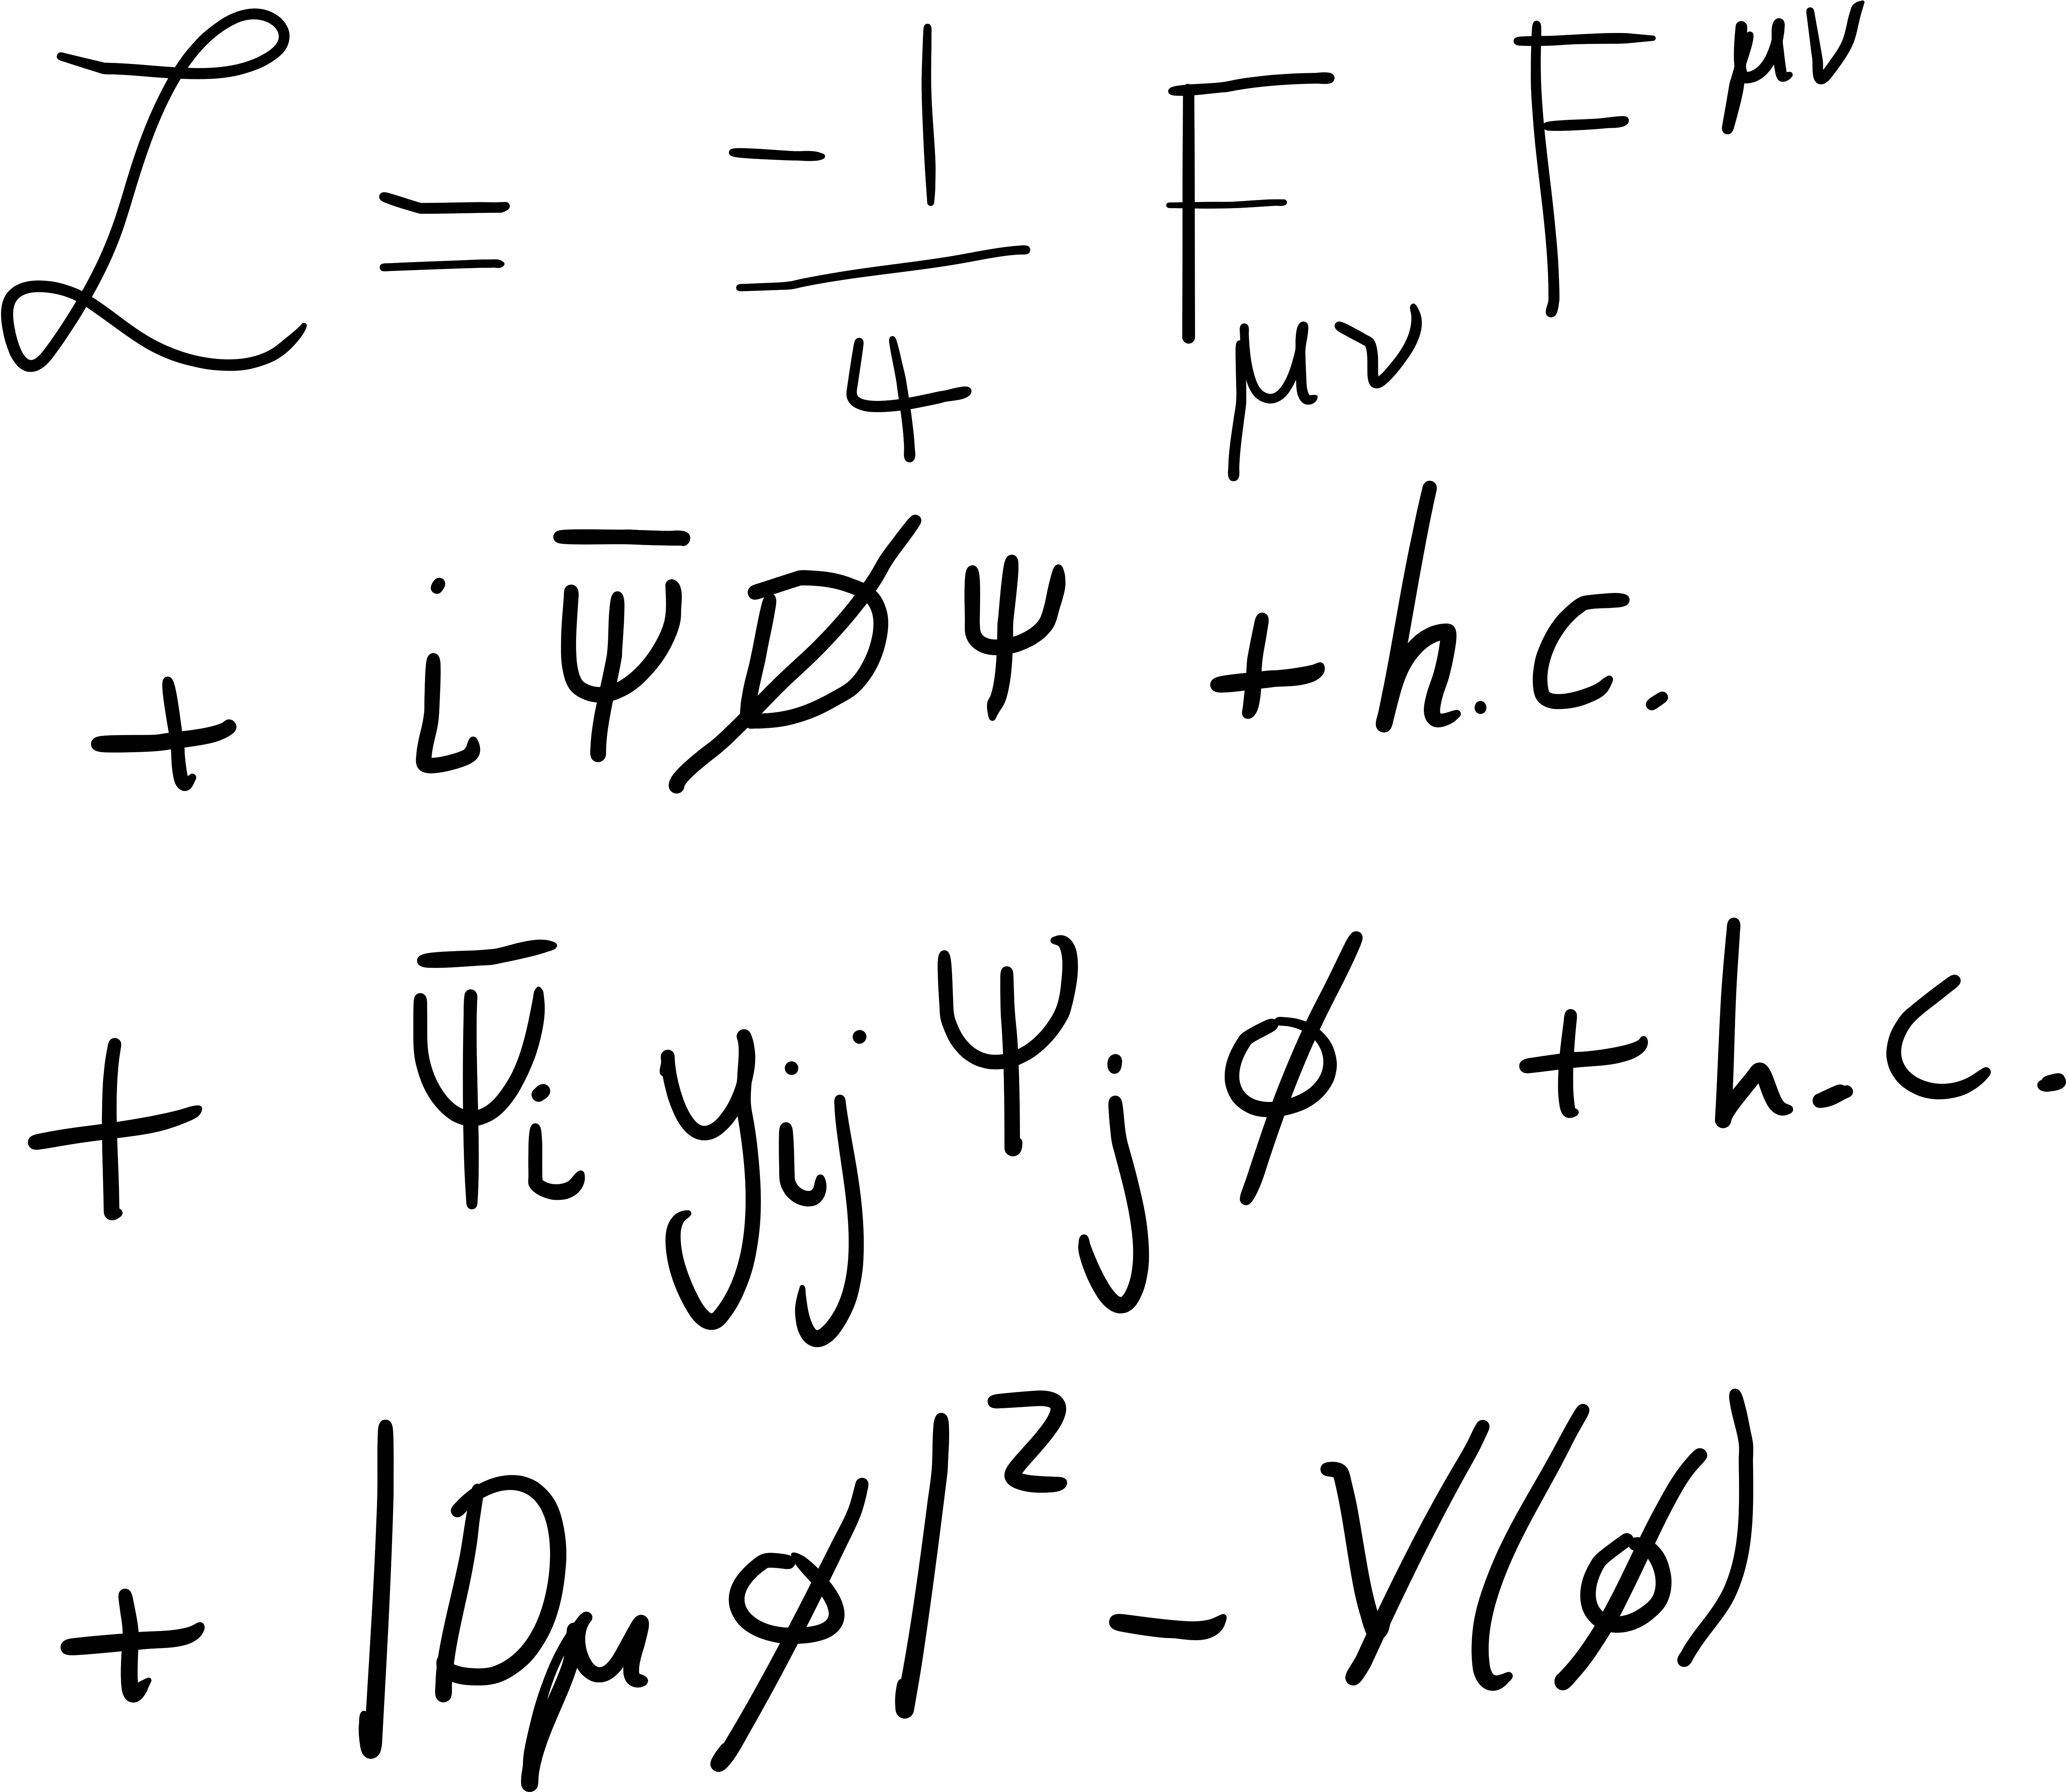
\includegraphics[width=.25\textwidth]{hand_written_lagrangian-1} \\Theory};
    
    \node [cloud, right=of root, align=left] (detector)  {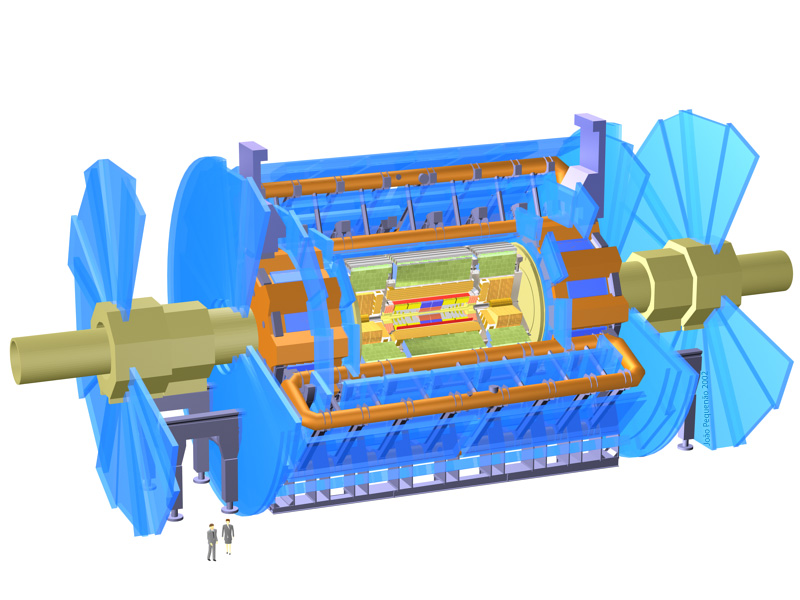
\includegraphics[width=.25\textwidth]{atlas_big} \\Detector};

    \node [cloud, below=of root, align=left] (recon)  {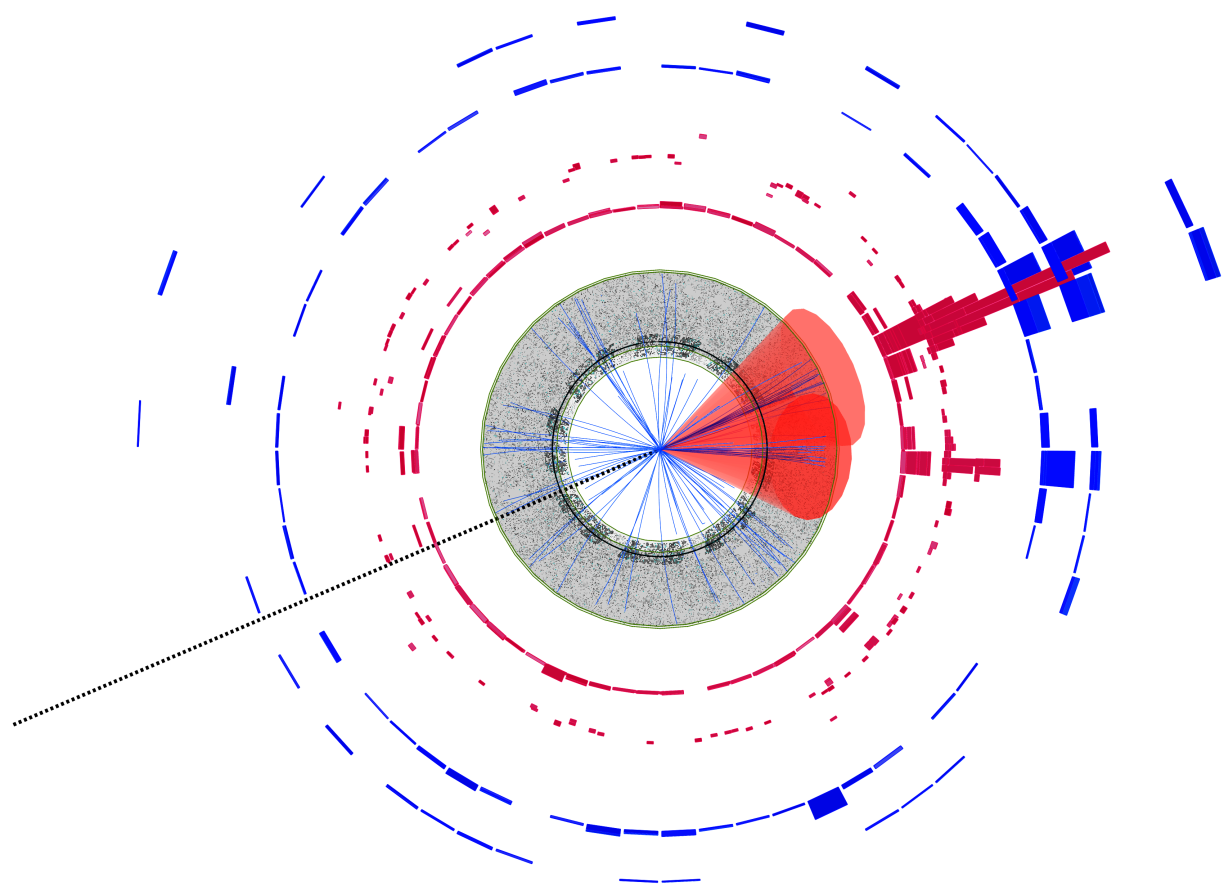
\includegraphics[width=.25\textwidth]{Event_Display_inv} \\Reconstruction};

    \node [cloud, below=of recon] (ghost1) {};
    
    \node [cloud, left=of ghost1, align=left] (modelling)  {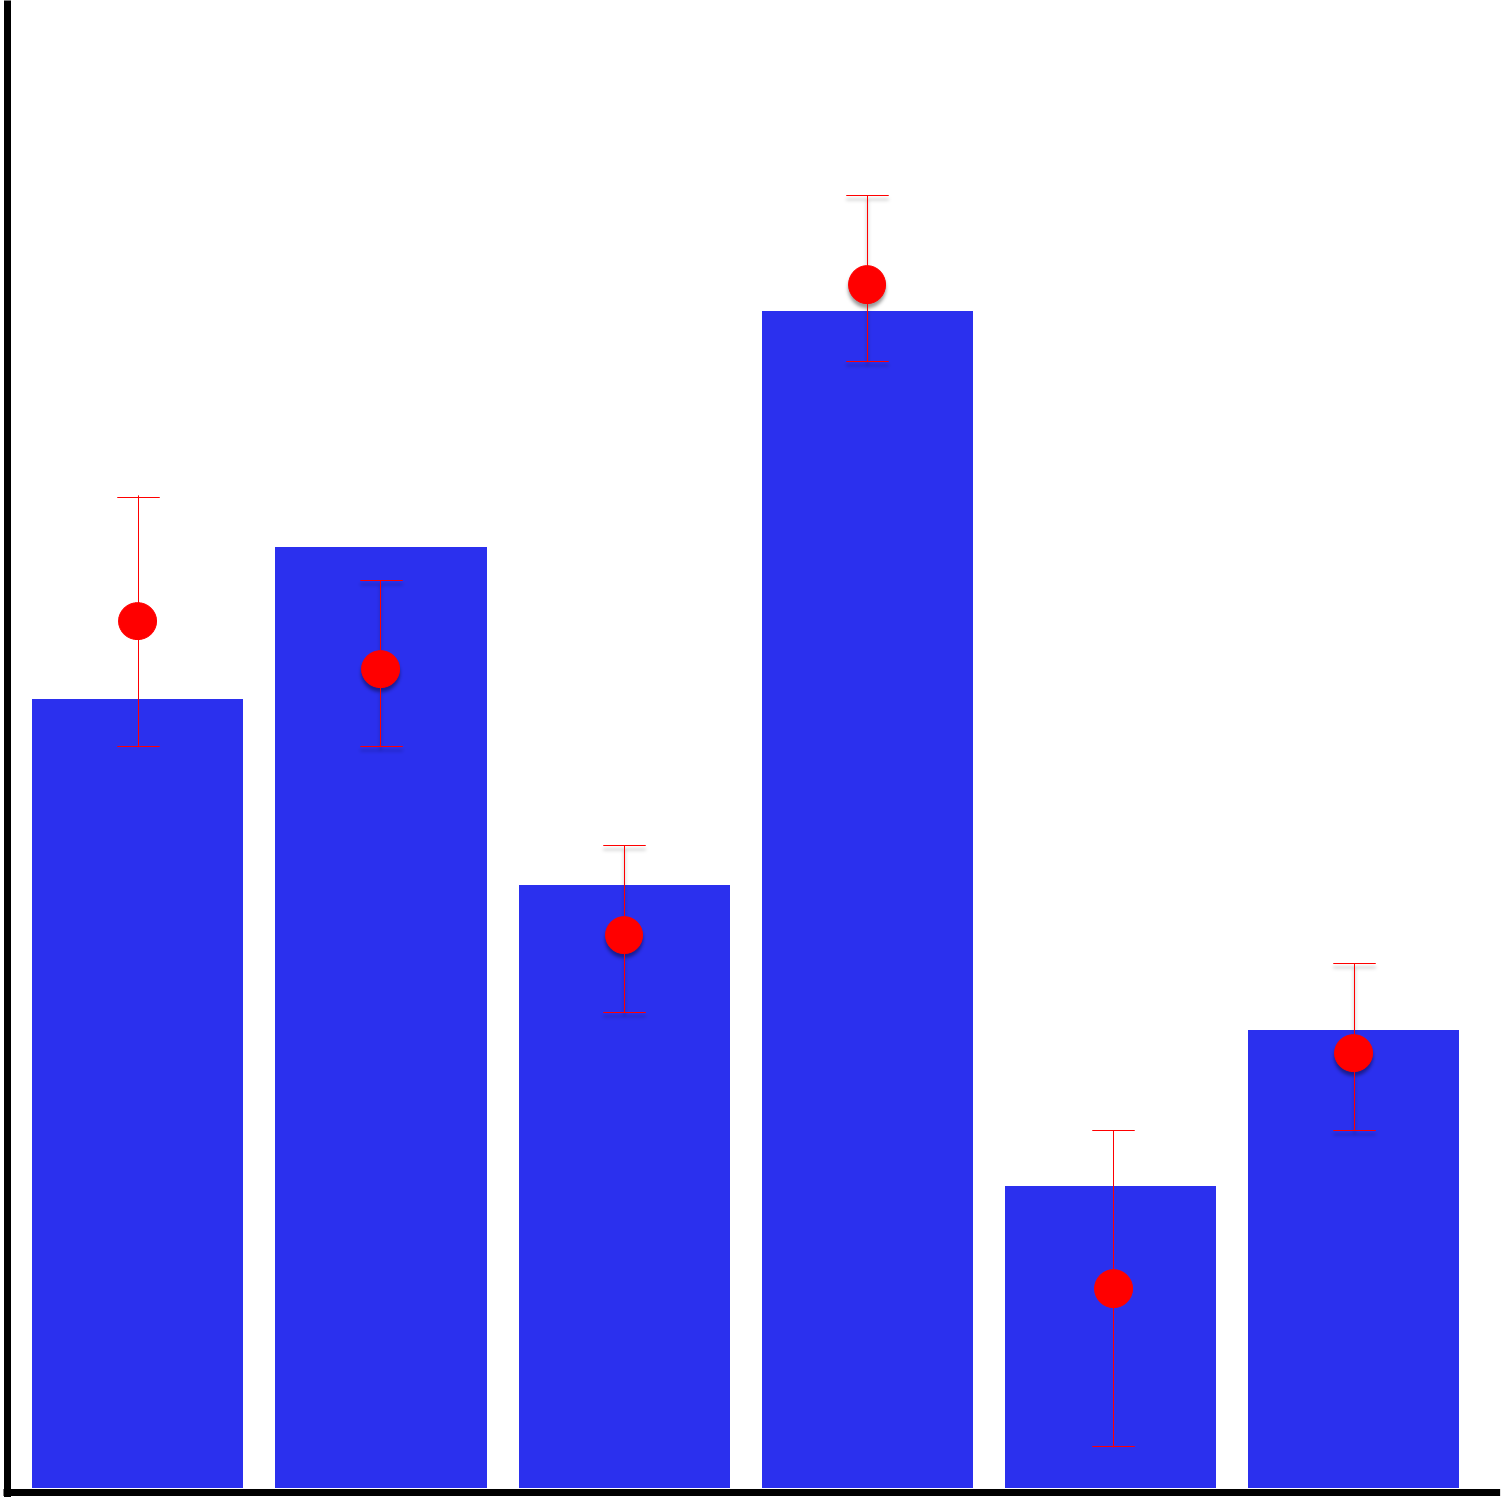
\includegraphics[width=.25\textwidth]{generic_data_mc} \\Modelling};

    \node [cloud, right=of ghost1, align=left] (mva)  {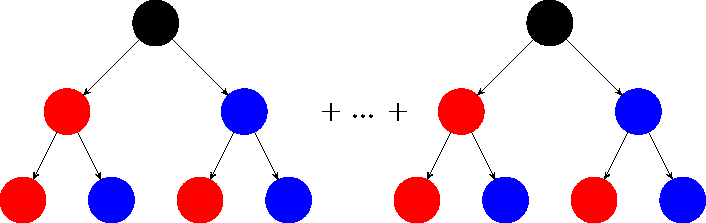
\includegraphics[width=.25\textwidth]{mini-bdt} \\Categorisation};

    \node [cloud, below=of ghost1, align=left] (plf)  {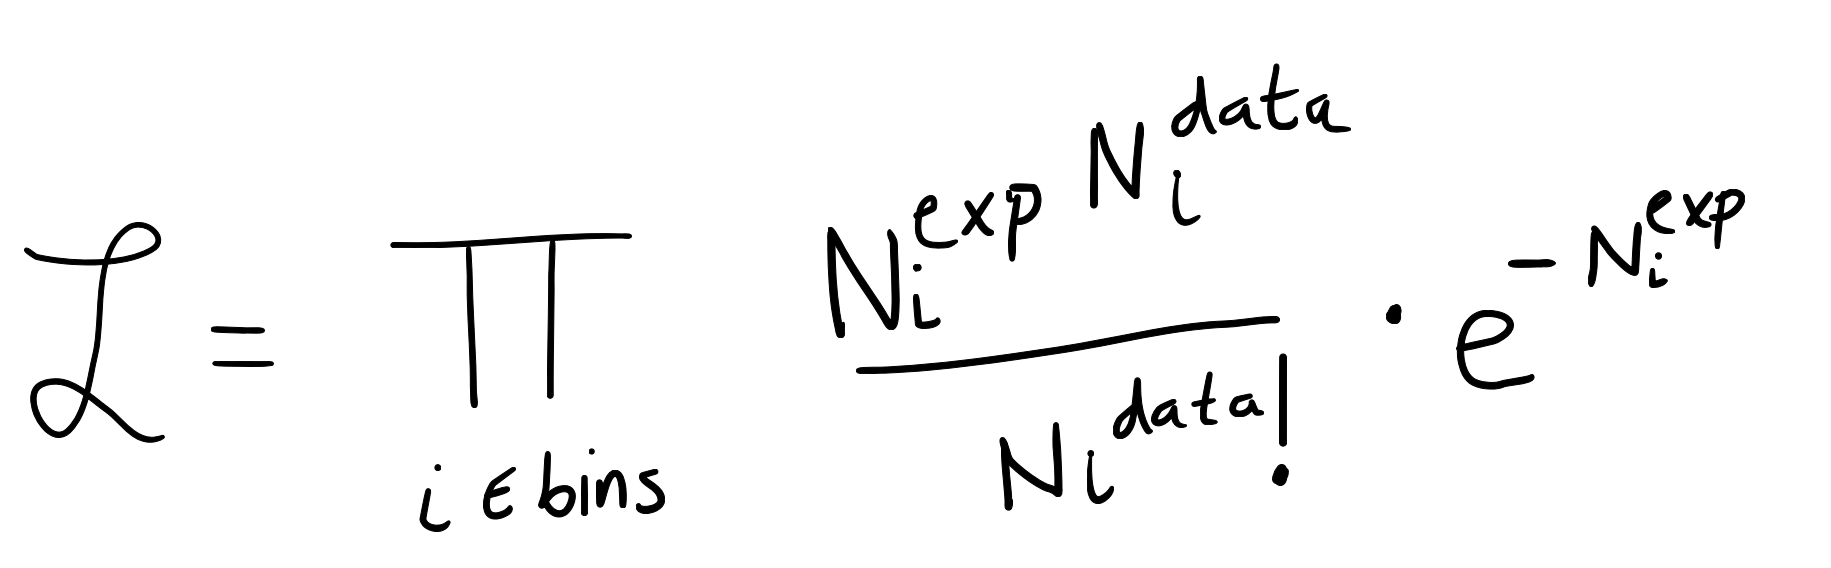
\includegraphics[width=.45\textwidth]{plf_handwritten} \\Profile-Likelihood Fit};

    \node [cloud, below=of plf, align=left] (results)  {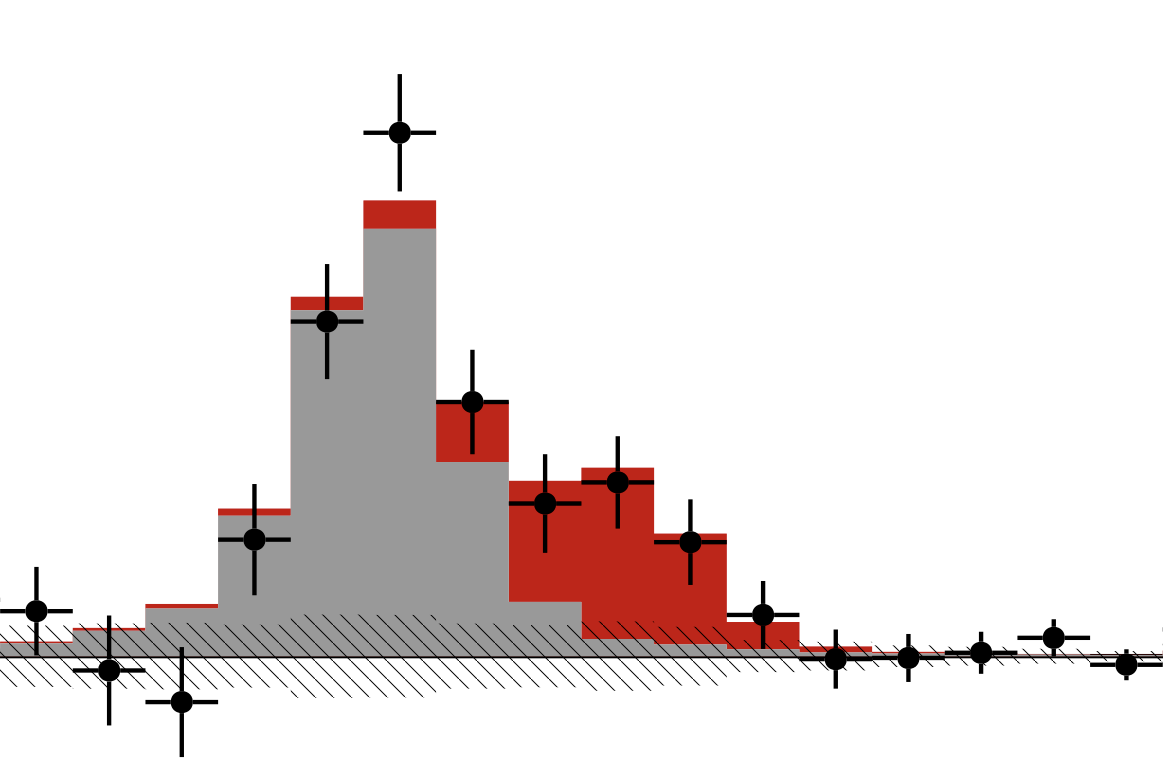
\includegraphics[width=.25\textwidth]{hbb_plot} \\Results \& Conclusions};
    
    % Draw edges 
    \path [line] (theory) -- (detector);

    \path [line] (detector) -- (recon);

    \path [line] (detector) to [out=200,in=70] (modelling);

    \path [line] (recon) -- (modelling);

    \path [line] (recon) -- (mva);

    \path [line] (mva) -- (plf);

    \path [line] (modelling) -- (plf);

    \path [line] (plf) -- (results);
    
  \end{tikzpicture}
  \caption[A roadmap of the analysis.]{A flow chart showing the roadmap of the \VHbb\ analysis and of this thesis.}
  \label{fig:roadmap}
\end{figure}
The blueprint starts with the theory of the Standard Model of Particle Physics,
described in chapter~\ref{ch:theory}. The theory's predictions inform the
design of the ATLAS detector which is detailed in chapter~\ref{ch:detector}.
Furthermore, the theory aids the choice of particles to collide, which events to
analyse, and allows us to generate predictions of what should happen in the
collisions. Chapter~\ref{ch:ml} gives an overview of two machine learning
algorithms that are used throughout the analysis. Events must be reconstructed
before they can be analysed, a selection process is used on the reconstructed
objects to filter events not relevant to the analysis. The reconstruction and
selection process is described in chapter~\ref{ch:recon}. Events in data must
be categorised into those that are signal-like and those that are
background-like in order to extract the most signal sensitivity from the
analysis. This is achieved with a number of strategies including a multi-variate
algorithm which is trained on the simulations. This categorisation process is
described in chapter~\ref{ch:strategy}, along with the overall analysis
strategy. A choice is made of simulated events that well model the data.
Considering the modelling, the theory and the shortcomings of the detector a set
of systematic errors are estimated, these are detailed in~\ref{ch:systematics}.
With the events categorised and the systematic errors on the counts in category
estimated, these counts serve as inputs to a profile-likelihood fit. Several fit
models exist to serve a number of purposes, the fit models are described in
chapter~\ref{ch:fit-models}. The results of the analysis are shown in
chapter~\ref{ch:results} and conclusions are drawn in
chapter~\ref{ch:conclusion}.


My contributions to the \VHbb\ analysis published in 2021 have been numerous and
spanned a number of different areas of the analysis.

My largest contribution was the derivation of new estimates of background
modelling uncertainties. This includes deriving new shape uncertainty estimates
for the $Z+$jets background in the 0 and 2 lepton channels which use a method
which includes a number of improvements over the previous analysis (explained in
detail in chapter~\ref{ch:systematics}). I also calculated estimates of
uncertainties arising due to differences in the flavour composition and yields
in given analysis regions between simulation and data for the $Z+$jets and top
backgrounds. I helped to develop and test code which performs a
multi-dimensional re-weighting of one dataset to another. This technique has
been used to estimate uncertainties of the top backgrounds and $W+$jets
backgrounds in the 1 lepton channel.

My next largest contribution was to studying the profile likelihood fit that
outputs the final analysis results. During key milestones of the analysis it is
often necessary to compare the blinded results of the fit to study the behaviour
of nuisance parameters and how they are pulled, constrained and correlated with
one another. I performed many of these comparisons paying close attention to the
nuisance parameters relating to the aforementioned estimates on background
modelling uncertainties. After approval was granted to unblind the analysis I
was also responsible for running the final fit for the diboson measurement which
serves as a cross-check of the all of the analysis methodology used for the
Higgs measurement.

Finally I have also made contributions to the general running of the analysis.
These including training the classification algorithm which provides the final
discriminating metric upon which the profile-likelihood fit is performed,
helping to maintain the analysis framework (which is also used by many other
ATLAS analyses) and participating in regular meetings with the analysis team
where ideas are discussed and the general analysis direction is decided.

\chapter{Physics Theory}%
\label{ch:theory}

The following chapter outlines the physics theory that informs and guides the
experimental process of searching for new particles or making measurements at a
particle collider. Not only are the physics theories described here useful in
that context but they also provide an almost complete picture of the universe at
certain scales. This chapter was written with the aid of notes taken at the
annual STFC High Energy Physics Summer School, and with the aid of several
books~\cite{halzen, thomson_2013}, in which a more detailed description of the
theories can be found.

The Standard Model of particle physics is a theoretical framework that describes
all elementary particles and three of the fundamental forces of nature. Notably
the only force that is not described by the theory is gravity. Particles
described by the model are listed in table~\ref{tab:sm} with a white gap
separating the matter particles (fermions) from the force carrying particles
(bosons). Fermions, which make up solid matter obey
Fermi-Dirac~\cite{Fermi-stat, Dirac-stat} statistics whereas bosons obey
Bose-Einstein~\cite{Bose-Einstein} statistics. The Higgs boson is special in
that as far as we know it does not carry a force in the conventional sense,
instead it is responsible for giving fundamental particles mass, discussed in
more detail in section~\ref{sec:higgs-mech}. In the table of particles quarks
(blue) and leptons (red) are ordered in columns by increasing mass, apart from
the neutrinos, which are massless in the theory. \begin{table}[ht]
  \centering
  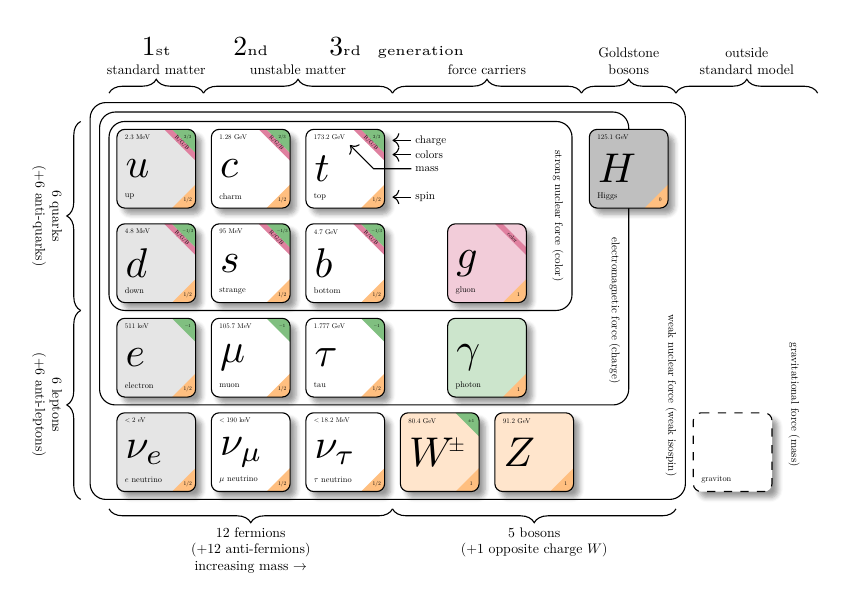
\begin{tikzpicture}[x=1.2cm, y=1.2cm]
  \draw[round] (-0.5,0.5) rectangle (4.4,-1.5);
  \draw[round] (-0.6,0.6) rectangle (5.0,-2.5);
  \draw[round] (-0.7,0.7) rectangle (5.6,-3.5);

  \node at(0, 0)   {\particle[gray!20!white]
                   {$u$}        {up}       {$2.3$ MeV}{1/2}{$2/3$}{R/G/B}};
  \node at(0,-1)   {\particle[gray!20!white]
                   {$d$}        {down}    {$4.8$ MeV}{1/2}{$-1/3$}{R/G/B}};
  \node at(0,-2)   {\particle[gray!20!white]
                   {$e$}        {electron}       {$511$ keV}{1/2}{$-1$}{}};
  \node at(0,-3)   {\particle[gray!20!white]
                   {$\nu_e$}    {$e$ neutrino}         {$<2$ eV}{1/2}{}{}};
  \node at(1, 0)   {\particle
                   {$c$}        {charm}   {$1.28$ GeV}{1/2}{$2/3$}{R/G/B}};
  \node at(1,-1)   {\particle 
                   {$s$}        {strange}  {$95$ MeV}{1/2}{$-1/3$}{R/G/B}};
  \node at(1,-2)   {\particle
                   {$\mu$}      {muon}         {$105.7$ MeV}{1/2}{$-1$}{}};
  \node at(1,-3)   {\particle
                   {$\nu_\mu$}  {$\mu$ neutrino}    {$<190$ keV}{1/2}{}{}};
  \node at(2, 0)   {\particle
                   {$t$}        {top}    {$173.2$ GeV}{1/2}{$2/3$}{R/G/B}};
  \node at(2,-1)   {\particle
                   {$b$}        {bottom}  {$4.7$ GeV}{1/2}{$-1/3$}{R/G/B}};
  \node at(2,-2)   {\particle
                   {$\tau$}     {tau}          {$1.777$ GeV}{1/2}{$-1$}{}};
  \node at(2,-3)   {\particle
                   {$\nu_\tau$} {$\tau$ neutrino}  {$<18.2$ MeV}{1/2}{}{}};
  \node at(3,-3)   {\particle[orange!20!white]
                   {$W^{\hspace{-.3ex}\scalebox{.5}{$\pm$}}$}
                                {}              {$80.4$ GeV}{1}{$\pm1$}{}};
  \node at(4,-3)   {\particle[orange!20!white]
                   {$Z$}        {}                    {$91.2$ GeV}{1}{}{}};
  \node at(3.5,-2) {\particle[green!50!black!20]
                   {$\gamma$}   {photon}                        {}{1}{}{}};
  \node at(3.5,-1) {\particle[purple!20!white]
                   {$g$}        {gluon}                    {}{1}{}{color}};
  \node at(5,0)    {\particle[gray!50!white]
                   {$H$}        {Higgs}              {$125.1$ GeV}{0}{}{}};
  \node at(6.1,-3) {\particle
                   {}           {graviton}                       {}{}{}{}};

  \node at(4.25,-0.5) [force]      {strong nuclear force (color)};
  \node at(4.85,-1.5) [force]    {electromagnetic force (charge)};
  \node at(5.45,-2.4) [force] {weak nuclear force (weak isospin)};
  \node at(6.75,-2.5) [force]        {gravitational force (mass)};

  \draw [<-] (2.5,0.3)   -- (2.7,0.3)          node [legend] {charge};
  \draw [<-] (2.5,0.15)  -- (2.7,0.15)         node [legend] {colors};
  \draw [<-] (2.05,0.25) -- (2.3,0) -- (2.7,0) node [legend]   {mass};
  \draw [<-] (2.5,-0.3)  -- (2.7,-0.3)         node [legend]   {spin};

  \draw [mbrace] (-0.8,0.5)  -- (-0.8,-1.5)
                 node[leftlabel] {6 quarks\\(+6 anti-quarks)};
  \draw [mbrace] (-0.8,-1.5) -- (-0.8,-3.5)
                 node[leftlabel] {6 leptons\\(+6 anti-leptons)};
  \draw [mbrace] (-0.5,-3.6) -- (2.5,-3.6)
                 node[bottomlabel]
                 {12 fermions\\(+12 anti-fermions)\\increasing mass $\to$};
  \draw [mbrace] (2.5,-3.6) -- (5.5,-3.6)
                 node[bottomlabel] {5 bosons\\(+1 opposite charge $W$)};

  \draw [brace] (-0.5,.8) -- (0.5,.8) node[toplabel]         {standard matter};
  \draw [brace] (0.5,.8)  -- (2.5,.8) node[toplabel]         {unstable matter};
  \draw [brace] (2.5,.8)  -- (4.5,.8) node[toplabel]          {force carriers};
  \draw [brace] (4.5,.8)  -- (5.5,.8) node[toplabel]       {Goldstone\\bosons};
  \draw [brace] (5.5,.8)  -- (7,.8)   node[toplabel] {outside\\standard model};

  \node at (0,1.2)   [generation] {1\tiny st};
  \node at (1,1.2)   [generation] {2\tiny nd};
  \node at (2,1.2)   [generation] {3\tiny rd};
  \node at (2.8,1.2) [generation] {\tiny generation};
\end{tikzpicture}
  % \begin{tabular}{|c|c|c|c|c|c|c|}
  %   %\multicolumn{6}{c}{\textbf{Particles of the Standard Model}}
  %   %\\
  %   \hhline{---|~|--}
  %   \cellcolor{blue!18} $u$ &
  %   \cellcolor{blue!18} $c$ &
  %   \cellcolor{blue!18} $t$ &
  %   ~ &
  %   \cellcolor{yellow!18} $g$ &
  %   \cellcolor{green!18} $H$
  %   \\
  %   \cellcolor{blue!18} \small{$up~quark$} &
  %   \cellcolor{blue!18} \small{$charm~quark$} &
  %   \cellcolor{blue!18} \small{$top~quark$} &
  %   ~ &
  %   \cellcolor{yellow!18} \small{$gluon$} &
  %   \cellcolor{green!18} \small{$Higgs$}
  %   \\
  %   \cline{1-3}
  %   \cline{5-6}
  %   %\hhline{~~~~~-}
  %   %\hhline{~~~~~|--|}
  %   \cellcolor{blue!18} $d$ &
  %   \cellcolor{blue!18} $s$ &
  %   \cellcolor{blue!18} $b$ &
  %   ~ &
  %   \cellcolor{yellow!18} $\gamma$
  %   \\
  %   \cellcolor{blue!18} \small{$down~quark$} &
  %   \cellcolor{blue!18} \small{$strange~quark$} &
  %   \cellcolor{blue!18} \small{$bottom~quark$} &
  %   ~ &
  %   \cellcolor{yellow!18} \small{$photon$}
  %   \\
  %   \hhline{---~|-|~}
  %   %\hline
  %   \cellcolor{red!18} $e^-$ &
  %   \cellcolor{red!18} $\mu^{-}$ &
  %   \cellcolor{red!18} $\tau^-$ &
  %   ~ &
  %   \cellcolor{yellow!18} $Z^0$
  %   \\
  %   \cellcolor{red!18} \small{$electron$} &
  %   \cellcolor{red!18} \small{$muon$} &
  %   \cellcolor{red!18} \small{$tau$} &
  %   ~ &
  %   \cellcolor{yellow!18} \small{$Z~boson$}
  %   \\
  %   \cline{1-3}
  %   \cline{5-5}
  %   \cellcolor{red!18} $\nu_{e}$ &
  %   \cellcolor{red!18} $\nu_{\mu}$ &
  %   \cellcolor{red!18} $\nu_{\tau}$ &
  %   ~ &
  %   \cellcolor{yellow!18} $W^\pm$
  %   \\
  %   \cellcolor{red!18} \small{$electron~neutrino$} &
  %   \cellcolor{red!18} \small{$muon~neutrino$} &
  %   \cellcolor{red!18} \small{$tau~neutrino$} &
  %   ~ &
  %   \cellcolor{yellow!18} \small{$W~boson$}
  %   \\
  %   \cline{1-3}
  %   \cline{5-5}
  % \end{tabular}
  \caption{The particles of the standard model with fermions displayed on the
    left and bosons on the right. Quarks are in blue, leptons in red, vector
    bosons in yellow and scalar bosons in green.}
  \label{tab:sm}
\end{table}


The model describes forces as being mediated by certain particles, the photon
($\gamma$) mediates the electromagnetic force, particles experiencing
electromagnetic repulsion or attraction are described as exchanging photons. The
strength and direction of the force experienced is proportional to the
electromagnetic charge of particles involved. The Standard Model is a theory of
quantum fields in which the strength of interactions between fields, or
particles which are described as excitations in the fields, is parametrised by
something known as a coupling constant. It is natural to assume that the
strength of the interaction between photons and charged particles is related to
the electromagnetic charge of the particles involved. Indeed this is the case
consider the Coulomb force between two protons,
\begin{equation} F = \frac{e^2}{4\pi\epsilon_0r},
\end{equation} where $e$ is the elementary charge, $\epsilon_0$ is the electric
constant and $r$ is the distance between the two protons in question and also
the energy of a photon given by
\begin{equation} E = \frac{hc}{\lambda},
\end{equation} where $h$ is Planck's constant, $c$ is the speed of light and
$\lambda$ is the wavelength of the photon. The value of the ratio of these two
quantities
\begin{equation}
  \label{eq:fine-structure} \alpha = \frac{e^{2}\lambda}{4\pi\epsilon_{0}rhc},
\end{equation} known as the fine structure constant, is the coupling constant
that describes the strength of the interactions between the photon field and
fields of particles with electromagnetic charge. So as is now clear this
coupling constant does indeed depend on the electromagnetic charge of the
objects involved and so it is not constant.

As well as the electromagnetic force the Standard Model describes the strong
nuclear force and the weak nuclear force, shortened to just the strong and weak
forces respectively. Like the electromagnetic force they too are mediated by the
exchange of particles, the gluons ($g$) carry the strong force and the $W^\pm$
and $Z^0$ bosons carry the weak force.

The charge associated with the strong force is known as colour which can take
values that are mapped onto colours in the visible spectrum (red, green, blue)
for ease of description. For each of these colours an anti-colour is also
allowed (anti-red, anti-green, anti-blue). Unlike with the electromagnetic
charge, particles with colour charge are not found freely in nature. Instead we
find particles known as hadrons which are bound states of quarks and anti-quarks
(e.g. the proton). The phenomenon of coloured particles being bound in such a
manner is known as colour confinement~\cite{colour-confinement}, and the bound
states are described by the quantum numbers isospin ($I$) and hypercharge
($Y_c$). It is commonly assumed that all free particles in nature are colour
singlets e.g. for a hadron the state could be written as
\begin{equation}
  \label{eq:hadron-colour} \frac{(r\bar{r} + b\bar{b} + g\bar{g})}{\sqrt{3}},
\end{equation} where $r$, $b$ and $g$ represent red, blue and green charges
respectively. This phenomenon is known as quark confinement. Gluons carry colour
and anti-colour indicating that there should be nine possible quantum mechanical
states for the gluon given the available number of colour/anti-colour
combinations, however when one considers that the strong force is exclusively
short range, and therefore that there should be no free gluons (disallowing
colour singlet gluons) the number of possible states is reduced to eight. The
state of a particle, as far as its description with respect to the strong force
is concerned, is given by a vector which lives in a vector space, in which
elements of the Lie group $SU(3)_C$ act as unitary operators, where the $C$
denotes that the group is associated with the colour charge. The $SU(3)$ group
is the group of $3~\times~3$ unitary matrices whose determinant is one.

Describing the weak force requires introducing further quantum numbers: weak
isospin $T$ and weak hypercharge $Y_W$. The state of a particle with regards to
the weak force is given by a vector which lives in a vector space in which
elements of $SU(2)_L \times $U(1)$_{Y_{W}}$ act as unitary operators where the
$L$ denotes that only particles in left-handed chiral states interact with the
weak force~\footnote{More specifically only left-handed chiral particles
participate in weak charged current interactions.}. Left-handed fermions are
represented as doublets in the theory with weak isospin $T = 1/2$ whilst
right-handed fermions are singlets with weak isospin $T = 0$.

Along the way we have described particle states with respect to particular
forces as vectors living in some vector space where the action of the element of
a group has been as a unitary operator. If we are to describe a particle state
taking into account the full model, the group whose elements should act as
unitary operators on the particle state (the gauge group) is $SU{(3)}_{C} \times
SU{(2)}_{L} \times U{(1)}_{Y_{W}}$. For each of the groups in the direct product
we have established a (gauge) symmetry and therefore due to Noether's
theorem~\cite{Noether_1971} there should be an associated conserved quantity.
The conserved quantities in this case are the electric charge, the weak
hypercharge and isospin and the colour charge.

\clearpage
\newpage

\section{Historical Aside}%
\label{sec:history}

This section provides some historical context surrounding the Dirac equation
which will later be used as the starting point in the discussion of quantum
electrodynamics, which is the sector of the Standard Model that describes
electromagnetic interactions.

In 1905 Albert Einstein first proposed the idea of special
relativity~\cite{Einstein:special}. The aim of the idea was to unify the then
inconsistent theories of Maxwell's electromagnetism and Newtonian mechanics. The
result of Einstein's work was a theory of motion which agreed with the
predictions of Newtonian mechanics at velocities much smaller than the speed of
light but whose predictions were accurate also at much higher velocities, for
which Newtonian predictions fail. A consequence of special relativity is that
it demands that any equation of motion must be invariant under Lorentz
transformations. Many physical phenomena predicted by special relativity could be
considered of high consequence in general, for example the phenomena of length
contraction, time dilation, energy-mass equivalence and the universal speed
limit equal to the speed of light in vacuum, all of which have been extensively
scrutinised experimentally ~\cite{sr-tests-1, sr-tests-2, sr-tests-3,
sr-tests-4, sr-tests-5, sr-tests-6, sr-tests-7}. It is the Lorentz
transformation however that should be kept in mind for the following discussion.
The transformation may be written as
\begin{equation}
  \begin{split}
    \begin{aligned}[t] &t'&=&\;\;\;\gamma(t -vx/c^{2}),\\
      &x'&=&\;\;\;\gamma(x - vt),\\
      \text{with } &\gamma&=&\;\;\;\frac{1}{\sqrt{1 - v^{2}/c^{2}}},
    \end{aligned}
  \end{split}
  \label{eq:lorentz-transform}
\end{equation} in a single dimension of space $x$ and one of time $t$ where $v$
represents the velocity of the system described by the primed coordinates
relative to the unprimed coordinates and $c$ is the speed of light in vacuum.

Twenty years after Einstein introduced the ideas of special relativity Erwin
Schr\"odinger postulated new ideas regarding the motion of quantum mechanical
systems~\cite{Schrodinger}. Though he knew his new equation was not invariant
under Lorentz transformations, and therefore incomplete, Schr\"odinger's
formulation of quantum mechanics changed the way physicists thought about the
universe forever. His famous equation
\begin{equation}
  \label{eq:schrodinger} i\hbar\frac{\partial}{\partial t}\Psi(\vec{x}, t) =
\Bigg(\frac{-\hbar^{2}}{2m}\nabla^{2} + V(\vec{x}, t) \Bigg)\Psi(\vec{x}, t),
\end{equation} describes the states of particles as wave-functions $\Psi$ which
can only be interpreted in a probabilistic manner and contains Planck's constant,
the quantum of action. This work had many consequences including the
quantisation of the values of measured observables (meaning they can only take
discrete values) and the descriptions of particles as waves.

It was the aim of Paul Dirac to make the Schr\"odinger equation Lorentz
invariant and thus provide a more complete description of quantum systems. Along
the way he came to the realisation that in order for his equation to satisfy
Lorentz invariance the wave-function had to be replaced with a four component
spinor ($\psi$) and the introduction of matrices known now as the Dirac matrices
(labeled $\gamma^{\mu} \text{ with } \mu=0,1,2,4$) was required. Though not the
form he originally wrote down, Dirac's Lagrangian density takes the form
\begin{equation}
    \label{eq:dirac} \mathcal{L}_{Dirac} =
\bar{\psi}(i\gamma^{\mu}\partial_{\mu} - m)\psi,
\end{equation} where the repeated up and down indices are implicitly summed
over $\partial_{\mu}$ represents the partial derivative taken with respect to a
spatial coordinate $\mu = 1,2,3$ or time $\mu = 0$.

\section{Quantum Electrodynamics}

In order to take Dirac's Lagrangian (eq. \ref{eq:dirac}) and turn it into
something that appropriately describes quantum electrodynamics (QED), we should
consider a $U(1)$ gauge transformation of the Dirac spinor and it's adjoint
\begin{equation}
  \label{eq:u1trans}
  \begin{split}
    \begin{aligned}[t] \psi \rightarrow &\psi' &=&\;\; e^{i\alpha(x)}\psi,\\
\bar{\psi} \rightarrow &\bar{\psi'} &=&\;\; e^{-i\alpha(x)}\bar{\psi},
    \end{aligned}
  \end{split}
\end{equation} with $\bar{\psi} \equiv \psi^{\dagger}\gamma^{0}$ and where
$\alpha(x)$ is a local phase. Under this transformation the Lagrangian
transforms as
\begin{equation}
  \label{eq:diracu1} \mathcal{L}_{Dirac} \rightarrow \mathcal{L}'_{Dirac} =
\bar{\psi}(i\gamma^{\mu}\partial_{\mu} - m)\psi -
\bar{\psi}\gamma^{\mu}\alpha(x)\psi
\end{equation} which is not equivalent to the original due to the factor
resulting from the derivative of the transformed spinor. Instead let us change
the derivative to the gauge covariant derivative
\begin{equation}
  \label{eq:covariant-em} D_\mu = \partial_{\mu} + ieA_{\mu},
\end{equation} where we interpret $A_{\mu}$ as the photon field, with coupling
constant $e$, parametrising the interaction strength. The field is also referred
to as the electromagnetic gauge field since it arrives during the process of
making the Lagrangian invariant under the $U(1)$ group, the gauge group of
electromagnetism. Note that here what we have labeled $e$ is nothing more than
the fine structure constant previously denoted $\alpha$ in eq.
\ref{eq:fine-structure}. The transformation of the new field under the action of
the gauge is defined as
\begin{equation}
  \label{eq:em-field-gauge} A_{\mu} \rightarrow A'_{\mu} \equiv A_{\mu} -
\frac{1}{e}\partial_{\mu}\alpha(x).
\end{equation} This means that the action of the gauge covariant derivative on
the spinor transforms as
\begin{equation}
  \label{eq:cov-trans} D_{\mu}\psi \rightarrow D'_{\mu}\psi' =
e^{i\alpha(x)}D_{\mu}\psi
\end{equation} which means that the new Lagrangian
\begin{equation}
  \label{eq:dirac-cov} \mathcal{L} = \bar{\psi}(i\gamma^{\mu}D_{\mu} - m)\psi
\end{equation} is invariant under the action of the gauge as desired. What
remains in order to write a description of QED is to write down a kinetic term
for the photon field. An appropriately gauge and Lorentz invariant term is
\begin{equation}
  \label{eq:em-kinetic} -\frac{1}{4}F_{\mu\nu}F^{\mu\nu}
\end{equation} where the electromagnetic tensor is defined as
\begin{equation}
  \label{eq:em-tensor} F_{\mu\nu} \equiv \partial_{\mu}A_{\nu} -
\partial_{\nu}A_{\mu}.
\end{equation}

Putting everything together we can define the Lagrangian for QED as
\begin{equation}
  \label{eq:qed} \mathcal{L}_{QED} = \bar{\psi}(i\gamma^{\mu}D_{\mu} - m)\psi
-\frac{1}{4}F_{\mu\nu}F^{\mu\nu}
\end{equation}

\section{Quantum Chromodynamics}

Quantum Chromodynamics (QCD) is the theory of the strong force. Its
mathematical formulation is similar to that of QED, except the gauge group for
QCD is $SU(3)_C$ where the $C$ denotes that the force is associated with colour
charge. As previously discussed the eight generators of the group are associated
with the eight gluons of the Standard Model. The generators are present in the
form of the transformation of a fermion field under an element of $SU(3)$
\begin{equation}
  \label{eq:su3-trans} \psi \rightarrow \psi' =
\exp\Big({i\alpha_{a}(x)\cdot\frac{\lambda_{a}}{2}}\Big)\psi,
\end{equation} where the $\lambda_a$ are the Gell-Mann matrices, generators of
$SU(3)$. A key difference between the strong force and the other forces
described by the Standard Model is that it increases in strength with range.
This is due to the fact that QCD is a non-Abelian gauge theory, meaning that the
gauge group has at least one pair of elements $a, b$ for which $a * b \neq b *
a$, where $*$ denotes the group multiplication operation. The consequence of
this is that the force carrier of the theory, the gluon carries a colour charge
and therefore can self-interact, resulting in the short range nature of the
strong force. This property leads to a phenomena known as quark confinement
which has been discussed previously. Quark confinement is the reason for many of
the complications that arise when trying to detect certain particles in a
particle detector such as ATLAS. Specifically, quarks and gluons that are
produced in collisions undergo a process called hadronisation whereby they
transition from their coloured states to colour singlets, producing a roughly
conical shower of particles known as a jet. Energy present in this process
results in the creation of lots of different states, some of which decay to
leptons.

\section{Electroweak theory}

The Glashow-Salam-Weinberg model of electroweak interactions~\cite{Glashow:1959,
Salam:1968, Weinberg:1967} describes the weak force and electromagnetism as a
quantum field theory, which is gauge invariant under transformations that are
elements of $SU{(2)}_{L} \times U{(1)}_{Y_{W}}$. As previously mentioned the $L$
and $Y_{W}$ subscripts denote that the gauge groups in the direct product that
are associated with left-handed chiral particles and weak hypercharge
respectively. The association with weak hypercharge distinguishes this $U(1)$
group with the $U(1)$ group from QED. The transformation of the fermion fields
under $SU(2)$ is given by
\begin{equation}
  \label{eq:su2-trans} \psi \rightarrow \psi' =
\exp\Big({i\vec{\alpha}(x)\cdot\frac{\vec{\sigma}}{2}}\Big)\psi,
\end{equation} where $\vec{\sigma}$ is a vector of the Pauli matrices
$\sigma_i\text{ with }i=1,2,3$, a familiar representation of $SU(2)$ generators.
Constructing a gauge covariant derivative for the full transformation under
$SU(2) \times U(1)$ requires the addition of new fields analogous to the photon
field from QED. The new derivative takes the form
\begin{equation}
  \label{eq:ew-derivative} D_{\mu} = \partial_{\mu} - i
\frac{g_1}{2}Y_{W}B_{\mu} - i\frac{g_2}{2}\sigma_{i}W_{\mu}^{i},
\end{equation} where coupling constants $g_1$ and $g_2$ parametrise the strength
of interactions with each field. The index $i$ runs over the three Pauli
matrices and three new fields $W^i_{\mu}\text{ with }i=1,2,3$ which are
associated with the $SU(2)$ gauge. The $B_{\mu}$ field is associated with the
$U(1)_{Y_{W}}$ gauge and is obtained in the same way as the photon field in QED
but is given a new symbol as it is \emph{not} the photon field.

In fact, none of the fields added here are the physical fields that we have
access to in nature associated with the electromagnetic force or the weak
currents. In order to obtain the physical fields for the weak charged current
one can simply take the linear superposition
\begin{equation}
  \label{eq:weak-charged-current} W_\mu^\pm = \frac{1}{\sqrt{2}}\big(W_\mu^{1}
\mp iW_\mu^2\big).
\end{equation} In order to recover the photon field and reveal the field for the
weak neutral current the idea of weak mixing must be introduced. Weak mixing was
introduced to the theory after the discovery of parity
violation~\cite{wu-parity}. Parity is an intrinsic property of a particle which
is similar to chirality. Chirality is not intrinsic to particles as a Lorentz
boost can always be appear to flip the chirality of the particles state. For
particles that are massless and therefore travelling at the speed of light this
cannot occur, for such particles chirality will always be equivalent to parity.
A fermion field with left or right handed chirality can be obtained by
multiplication with one of two corresponding projection operators defined as
\begin{equation}
  \begin{split}
    \begin{aligned}[t] P_L = {(1 - \gamma^{5})}^{2} / 2, \\ P_R = {(1 +
\gamma^{5})}^{2} / 2,
    \end{aligned}
  \end{split}
\end{equation} with $\gamma^{5} = i\gamma^{0}\gamma^{1}\gamma^{2}\gamma^{3}$,
where $\gamma^{\mu}$ are the Dirac matrices:
\begin{equation}
  \label{eq:chiral-fermions}
  \begin{split}
    \begin{aligned}[t] \psi_{L} = P_{L}\psi,\\ \psi_{R} = P_{R}\psi.
    \end{aligned}
  \end{split}
\end{equation} It is known that the weak neutral current and the electromagnetic
force both interact with particles of left and right handed chirality.
Spontaneous symmetry breaking has the effect of rotating the plane defined by
the $B_\mu$ and $W_\mu^3$ fields into the physical fields we see in nature
today. The mixing of the fields due to this rotation takes the form
\begin{equation}
  \label{eq:ew-mixing}
  \begin{pmatrix} A_\mu \\ Z_\mu
  \end{pmatrix} =
  \begin{pmatrix} \cos{\theta_W} & \sin{\theta_W} \\ -\sin{\theta_W} &
\cos{\theta_W}
  \end{pmatrix}
  \begin{pmatrix} B_\mu \\ W_\mu^3
  \end{pmatrix},
\end{equation} where $\theta_W$ the weak mixing angle parametrises the amount of
mixing. This picture shows that unification of QED, up to the inclusion of the
two coupling constants, and a description of the weak force has been achieved.
At first seems like the $U(1)_{EM}$ gauge group is not present in
$SU(2)_{L} \times U(1)_{Y_{W}}$ gauge group of electroweak theory it has been
shown~\cite{halzen} that the QED gauge symmetry is recovered by spontaneous
symmetry breaking. Also the $Y_W$ subscript in the gauge group represents weak
hypercharge which is related to electric charge $Q$ by the following
relationship
\begin{equation} Y_W = 2(Q - T^3),
\end{equation} where $T^3$ is the third component of isospin, the component that
must be conserved in weak interactions according to the theory.

The particles associated with the weak neutral and charged currents are observed
to have masses in nature~\cite{w-ua1, w-ua2, z-ua1, z-ua2} therefore one would
naively like to write mass terms of the form
\begin{align} \mathcal{L}_{mass} &\propto M^{2}_{B}B^{\mu}B_{\mu} \\ &+
M^{2}_{W}W^{\mu}_{a}W^{a}_{\mu}.
\end{align} The above mass terms are however not gauge invariant therefore
another solution is required, as the masses as observables which would be have
ambiguous predictions were they to change under gauge transformation.


\section{The Brout-Englert-Higgs Mechanism}%
\label{sec:higgs-mech}

The Brout-Englert-Higgs mechanism was made complete almost simultaneously by
R.~Brout and F.~Englert, P.~Higgs and, G.~Guralnik, C.~R.~Hagen and T.~Kibble.
The underlying mechanism was proposed prior to this work by
P.~Anderson~\cite{Anderson}, though this initial theory was not relativistic
invariant. It was initially proposed as a means to give the vector bosons mass
terms that were gauge invariant. The theory predicts a complex scalar field (the
Higgs field) that undergoes spontaneous symmetry breaking. Interactions with
this field are predicted to be mediated by a massive spin-1 scalar particle that
is now known to be the Higgs boson. This particle also gives mass to the
fermions via a different mechanism. In general spontaneous symmetry breaking is
a process by which a symmetry breaks once conditions meet some threshold. An
example of this is a hot sphere of ferromagnetic material whose spins are
isotropically oriented. As the sphere cools the ferromagnetic property of the
material will align the spins. In the hot scenario the sphere had symmetry in
all spatial directions, by this it is meant that the changes to the sphere's
orientation were indistinguishable. Once the spins have aligned however this is
no longer the case, the fact that the spins point in a specific direction means
that direction is special and so some of the symmetry was spontaneously broken.
It can be noted though that a preserved symmetry still exists as rotations about
the axis defined by the direction of the spins would leave the sphere invariant.
In the Standard Model the symmetry that breaks is that of the complex scalar
Higgs potential. Consider a Lagrangian involving the field $\phi$ of the form
\begin{gather} \mathcal{L} = T - V ( \phi ) = \partial_{\mu} \phi^{\dagger}
\partial^{\mu} \phi - \mu^{2} \phi^{\dagger} \phi + \lambda {( \phi^{\dagger}
\phi)}^{2}, \\ \text{with}~\phi =\frac{1}{\sqrt{2}}(\phi_{1} + i\phi_{2}).
\end{gather} Invariance under global phase transformations of the form
$\phi~\rightarrow~e^{i\theta}\phi$ depends on the parameters of the potential
$\mu$ and $\lambda$. Figure~\ref{fig:higgs-pot-01} shows two sketches of the
potential for the scenarios where $\mu^{2} > 0,~\lambda < 0$ (left) and $\mu^{2}
< 0,~\lambda < 0$ (right). \begin{figure}[h]
  \centering
  \subfloat[]{
  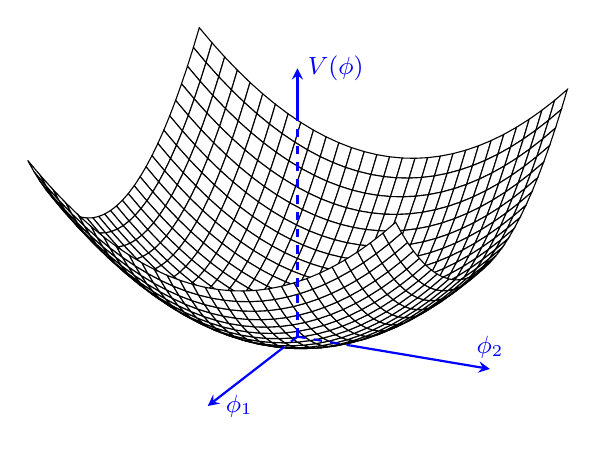
\begin{tikzpicture}%[scale=0.85]
    \begin{axis}[
        hide axis,
        %axis lines=middle,
        %            axis on top,
        %            axis line style={blue,dashed,thick},
        %            ymin=-2,ymax=2,
        %            xmin=-2,xmax=2,
        %            zmin=-2,zmax=2,
        samples=30,
        domain=-0.9:0.9,
        y domain=-0.9:0.9,clip=false
      ]
      \addplot3 [surf, shader=flat, draw=black, fill=white, z buffer=sort]
      ({0.85*x},{0.85*y},{0.85*x^2+y^2});
      \draw[blue,thick,dashed] (axis cs:0,0,0) -- (axis cs:0.22,0,0);
      %node[below,font=\small]{$\phi_{\text{IM}}$};
      \draw[blue,thick,-stealth] (axis cs:0.22,0,0) -- (axis cs:0.8,0,0)
      node[above,font=\small]{$\phi_{2}$};
      \draw[blue,thick,dashed] (axis cs:0,0,0) -- (axis cs:0,-0.15,0);
      %node[left=2mm,font=\small]{$\phi_{\text{RE}}$};
      \draw[blue,thick,-stealth] (axis cs:0,-0.15,0) -- (axis cs:0,-0.8,0)
      node[right=1mm,font=\small]{$\phi_{1}$};
      \draw[blue,thick,dashed] (axis cs:0,0,0) -- (axis cs:0,0,1.55);
      \draw[blue,thick,-stealth] (axis cs:0,0,1.55) -- (axis cs:0,0,1.9)
      node[right,font=\small]{$V(\phi)$};
    \end{axis}
  \end{tikzpicture}}
  \hspace{15mm}
  \subfloat[]{
  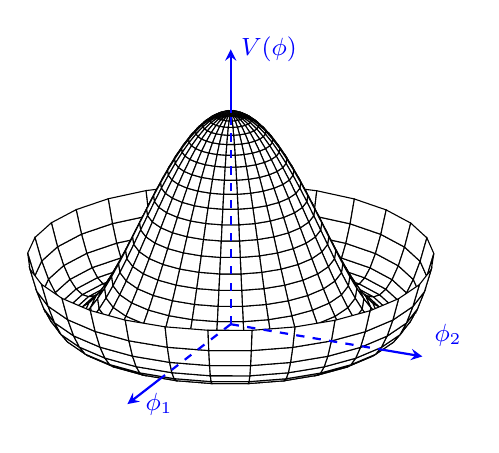
\begin{tikzpicture}
    \begin{axis}[
        hide axis,
        %axis lines=middle,
        %            axis on top,
        %            axis line style={blue,dashed,thick},
        %            ymin=-2,ymax=2,
        %            xmin=-2,xmax=2,
        %            zmin=-2,zmax=2,
        samples=30,
        domain=0:360,
        y domain=0:1.25,clip=false
      ]
      \addplot3 [surf, shader=flat, draw=black, fill=white, z buffer=sort]
      ({sin(x)*y}, {cos(x)*y}, {(y^2-1)^2});
      \draw[blue,thick,dashed] (axis cs:0,0,0) -- (axis cs:1,0,0);
      %node[below,font=\small]{$\phi_{\text{IM}}$};
      \draw[blue,thick,-stealth] (axis cs:1,0,0) -- (axis cs:1.3,0,0)
      node[above,font=\small]{~~~~~~$\phi_{2}$};
      \draw[blue,thick,dashed] (axis cs:0,0,0) -- (axis cs:0,-1,0);
      %node[left=2mm,font=\small]{$\phi_{\text{RE}}$};
      \draw[blue,thick,-stealth] (axis cs:0,-1,0) -- (axis cs:0,-1.5,0)
      node[right=1mm,font=\small]{$\phi_{1}$};
      \draw[blue,thick,dashed] (axis cs:0,0,0) -- (axis cs:0,0,1)
      %node[left=2mm,font=\small]{$\phi_{\text{RE}}$}
      ;
      \draw[blue,thick,-stealth] (axis cs:0,0,1) -- (axis cs:0,0,1.3)
      node[right,font=\small]{$V(\phi)$};
    \end{axis}
  \end{tikzpicture}}
  \caption{The Higgs potential in its fully and broken symmetric forms.}
  \label{fig:higgs-pot-01}
\end{figure}
 To suggest that
in our universe this symmetry is spontaneously broken is to suggest that the
values of these parameters evolved over time from the full to the broken state.
This ends up leading to masses for the vector bosons that are dependent on
$\mu^2$.

\section{Higgs Bosons at the LHC}
%
Higgs bosons are produced at the LHC in a number of different ways, the four
most common of which are shown in figure~\ref{fig:feyn-higgs-prod}.
\begin{figure}[ht]
  \centering
  \subfloat[]{
    \feynmandiagram [horizontal=a to b, yscale=0.9, xscale=0.8] {
      i1 [particle=\(g\)] -- [gluon] d -- [fermion, edge label=\(t\)] c -- [gluon] i2 [particle=\(g\)],
      i1 -- [draw=none] i2, 
      d -- [anti fermion, edge label=\(t\)] a -- [anti fermion, edge label=\(\overline{t}\)] c,
      a -- [scalar] b [particle=\(H^{0}\)],
    };
  }
  %\hspace{5.5mm}
  \subfloat[]{
    \feynmandiagram [horizontal=s to b, yscale=0.675, xscale=0.9] {
      i1 [particle=\(q_{1}\)] -- w1 -- f1 [particle=\(q_{2}\)],
      i2 [particle=\(q_{3}\)] -- w2 -- f2 [particle=\(q_{4}\)],
      s -- [draw=none] a,
      i1 -- [draw=none] s -- [draw=none] i2,
      w2 -- [photon] a -- [photon] w1,
      f1 -- [draw=none] b -- [draw=none] f2,
      a -- [scalar, edge label=\(H^{0}\)] b,
    };
  }
  %\vspace{1mm}
  \subfloat[]{
    \feynmandiagram [horizontal=a to b, scale =0.9] {
      i1 [particle=\(q\)] -- [fermion] a -- [fermion] i2 [particle=\(\overline{q}\)],
      a -- [photon, edge label=\(V\)] b,
      f1 [particle=\(V\)] -- [photon] b -- [scalar] f2 [particle=\(H^{0}\)],
    };
  }
  %\hspace{15mm}
  \subfloat[]{
    \feynmandiagram [horizontal=s to b, yscale=0.675, xscale=0.9] {
      i1 [particle=\(g\)] -- [gluon] q1 -- [anti fermion] f1 [particle=\(\overline{t}\)],
      i2 [particle=\(g\)] -- [gluon] q2 -- [fermion] f2 [particle=\(t\)],
      s -- [draw=none] a,
      i1 -- [draw=none] s -- [draw=none] i2,
      q2 -- a -- q1,
      f1 -- [draw=none] b -- [draw=none] f2,
      a -- [scalar, edge label=\(H^{0}\)] b,
    };
  }
  \caption{The four most common Higgs boson production methods from proton-proton collisions at the LHC.}
  \label{fig:feyn-higgs-prod}
\end{figure}
 The production cross-section of these
processes with respect to the centre of mass energy of the proton-proton
collision is shown in figure~\ref{fig:higgs-br} (a). It can be seen gluon-gluon
fusion (fig~\ref{fig:feyn-higgs-prod}~a) is by far the dominate contributor
occurring over an order of magnitude more than the next highest process which is
quark associated production (fig~\ref{fig:feyn-higgs-prod}~b). The next highest
production channel with respect to cross section is vector boson associated
(fig~\ref{fig:feyn-higgs-prod}~c) which will be the focus of the rest of this
report. Finally, top quark associated production
(fig~\ref{fig:feyn-higgs-prod}~d) has the smallest cross section of these
processes. The Higgs boson is predicted by the Standard Model to decay in a
number of different ways depending on its mass, a free parameter of the model.
In figure~\ref{fig:higgs-br} (b) the branching ratios of the Higgs can be seen,
plotted with respect to Higgs mass. The decay that will be focused on for the
rest of this report is a Higgs boson decaying to a pair of $b$-quarks, denoted
\Hbb.
\begin{figure}[ht]
  \centering
  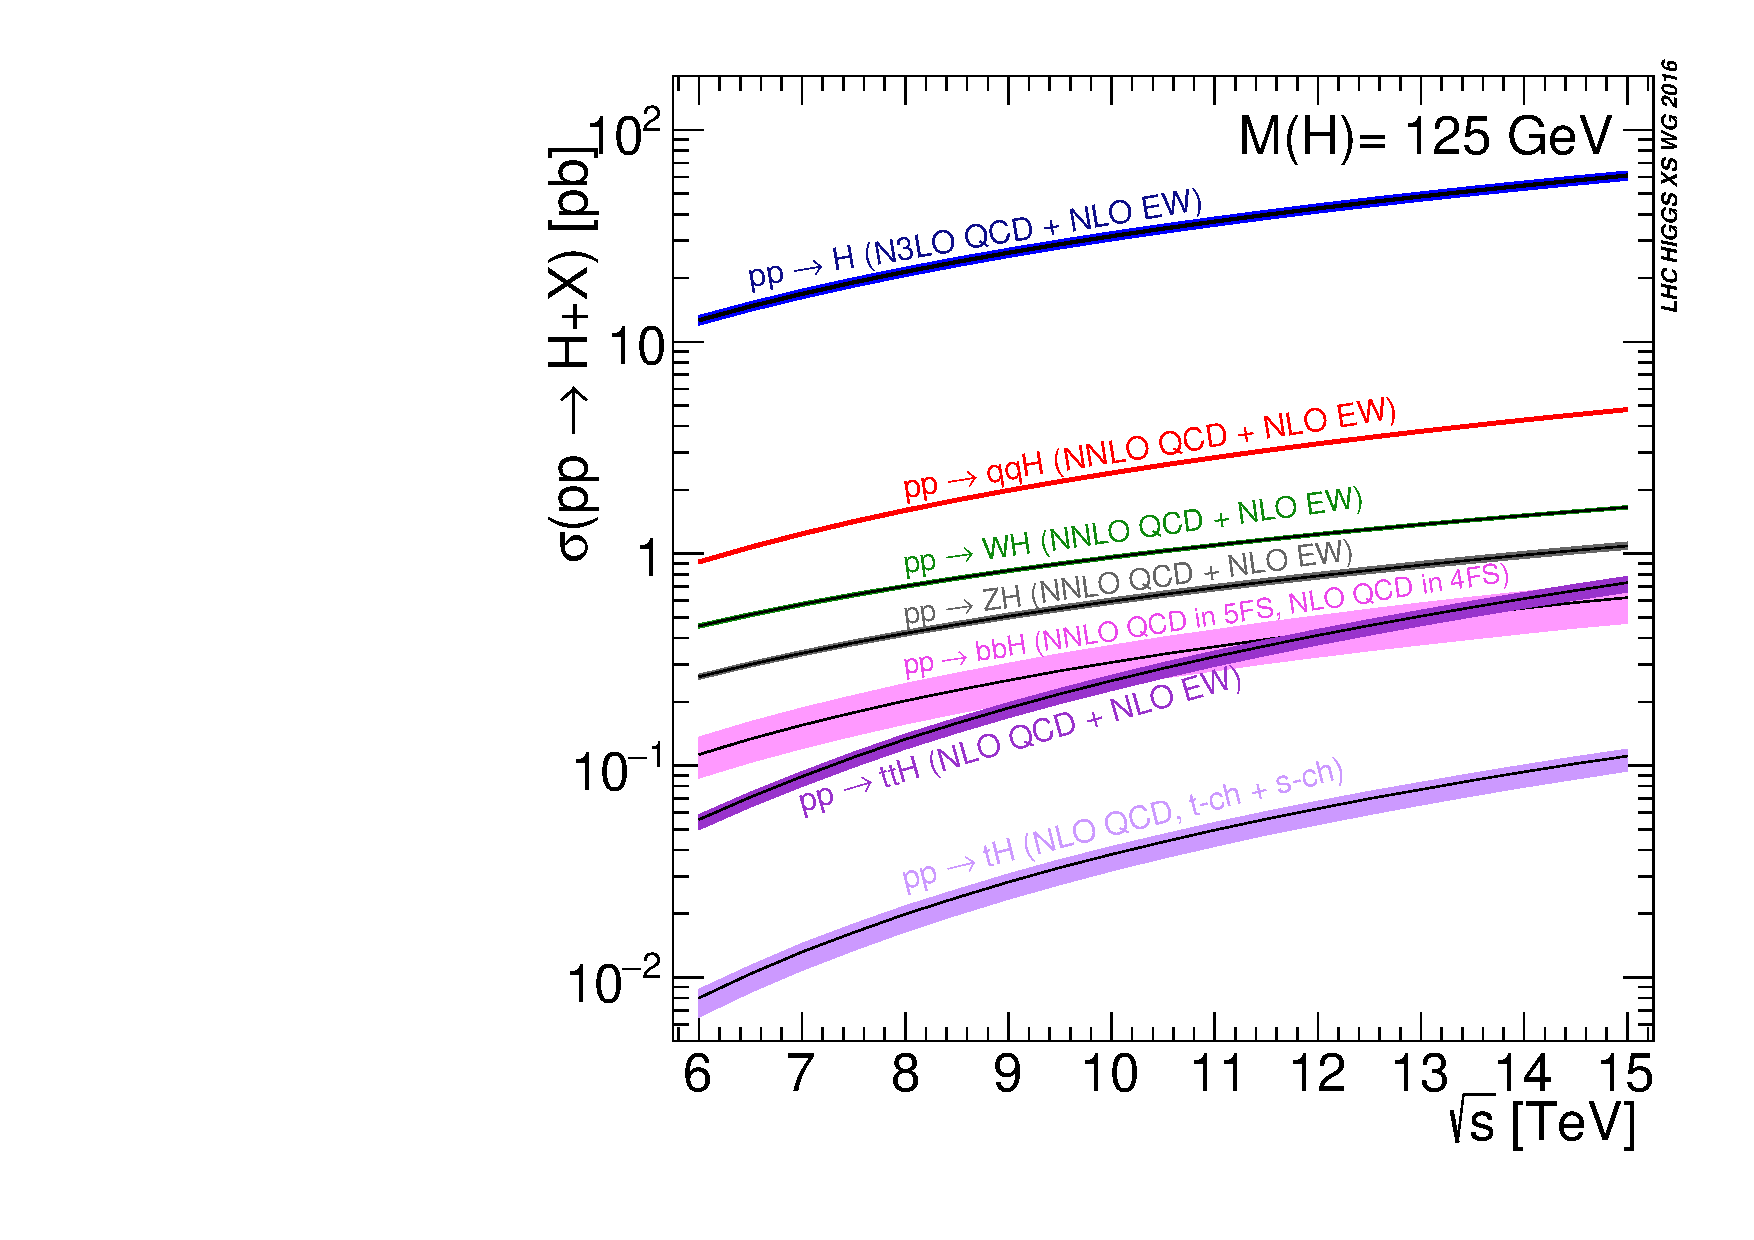
\includegraphics[width=.45\textwidth]{Plot_Escan_H125_xsec}%
  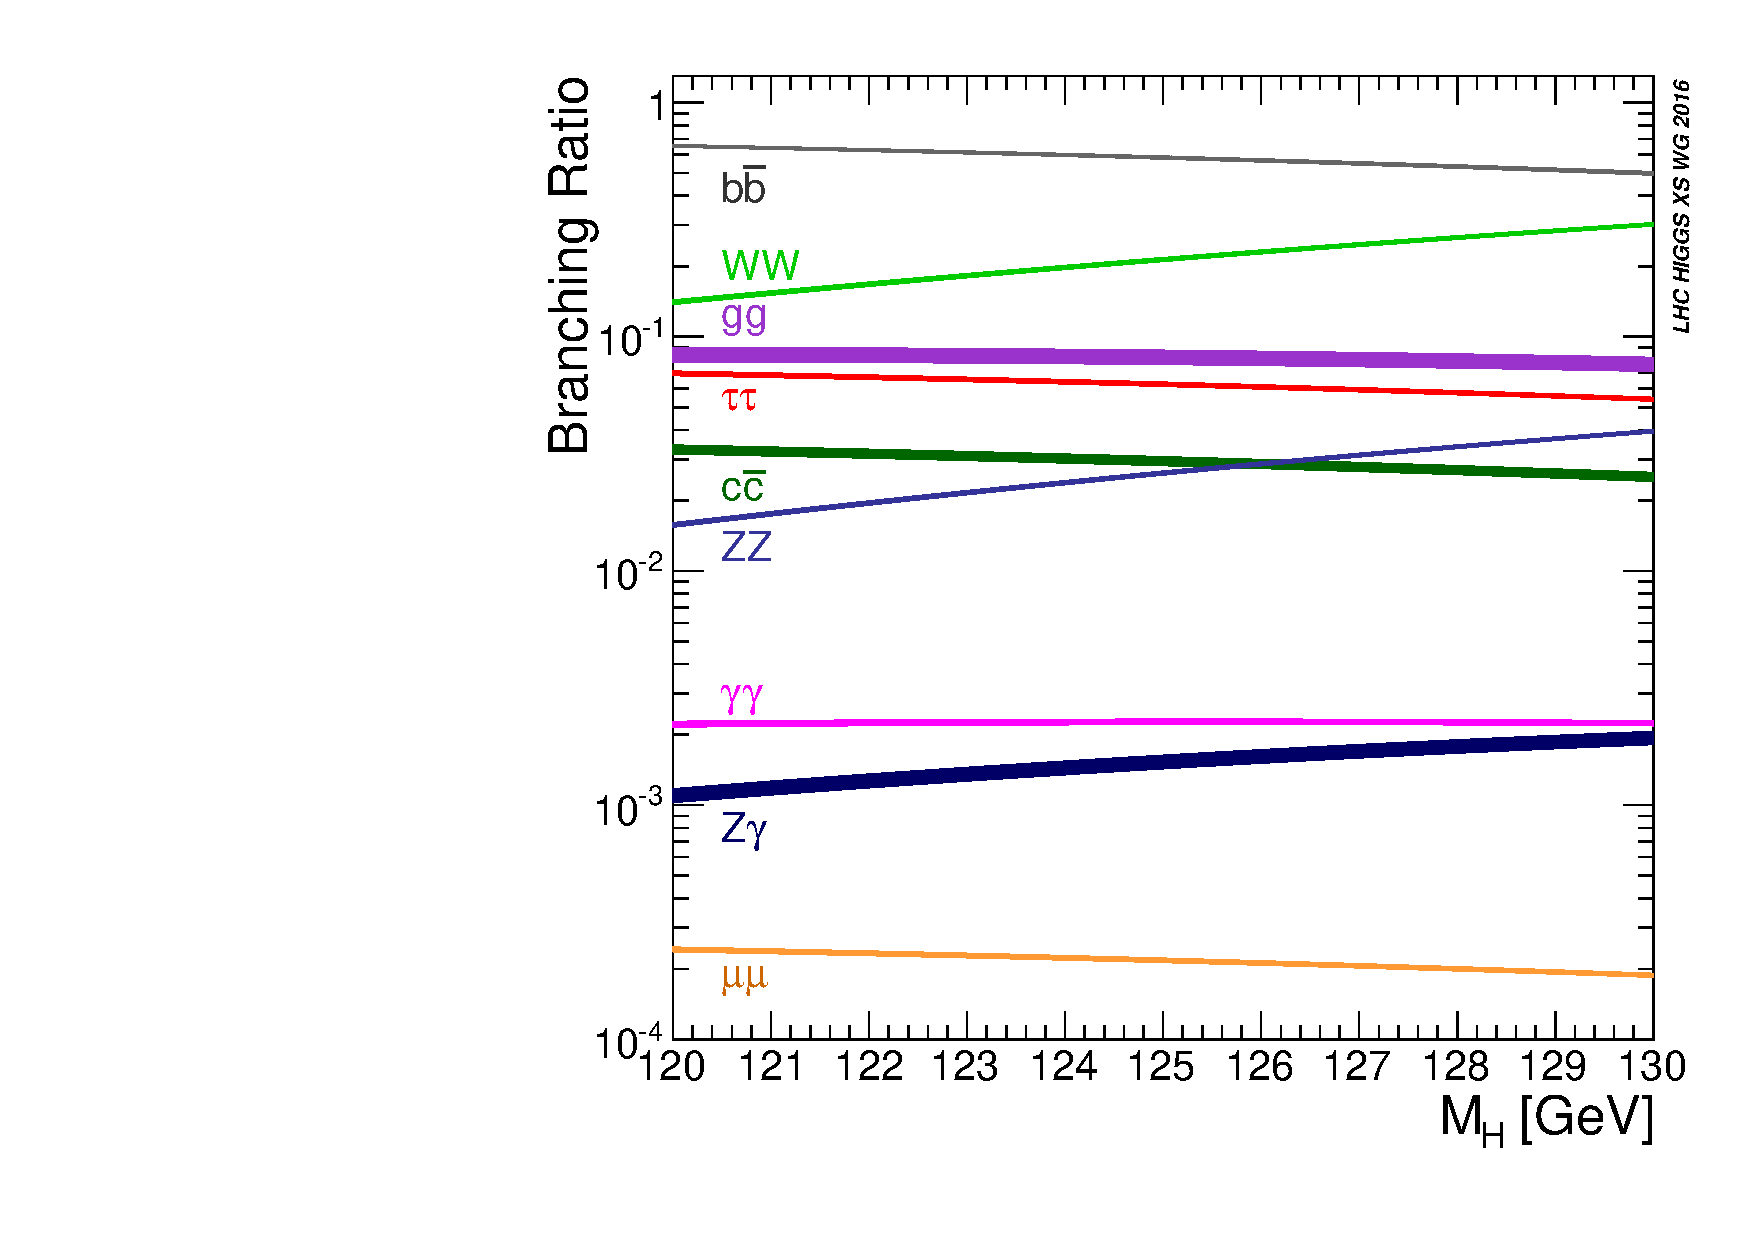
\includegraphics[width=.45\textwidth]{HiggsBR_mhscan}

  \caption[Higgs boson production cross sections and branching ratios.]{Higgs
    boson production cross-sections (left), and branching ratios (right) for a range
    of centre of meass energies and Higgs boson masses
    respectively~\cite{CERN-yellow-4}.}%
  \label{fig:higgs-br}
\end{figure}%
Given that the focus here is on vector boson associated production
of a Higgs boson it is also important to consider the decay of the vector boson.
Three possible scenarios are represented in figure~\ref{fig:feyn-vhbb}, namely
the situations where the vector boson decays to 0, 1 or 2 charged leptons and
the appropriate number of neutrinos. \begin{figure}
  \centering
  \feynmandiagram [horizontal=a to f] {
    i1 [particle=\(q\)] -- [fermion] a -- [fermion] i2 [particle=\(\overline{q}\)],
    a -- [photon, edge label=\(V\)] b -- [draw=none] f,
    w1 -- [photon, edge label=\(V\)] b -- [scalar, edge label=\(H^{0}\)] h1,
    l [particle=\(\ell^{+}/\overline{\nu}\)] -- [fermion] w1 -- [fermion] nu [particle=\(\ell^{-}/\nu\)],
    b1 [particle=\(\overline{b}\)] -- [fermion] h1 -- [fermion] b2 [particle=\(b\)],
    b2 -- [draw=none] f -- [draw=none] nu,
    h1 -- [draw=none] f -- [draw=none] w1,
  };
  \caption{A diagram showing a Higgs boson (decaying to a pair of b quarks) produced in association with a vector
    boson (decaying to 0, 1, or 2 charged leptons denoted $\ell^{+/-}$).
  }
  \label{fig:feyn-vhbb}
\end{figure}
 It is
these leptonic decay modes that motivate the reason for studying this production
mechanism as opposed to one of the more common ones. The issue with looking at
the other production modes is that very large QCD generated backgrounds are
present due to initial state radiation. Whilst these backgrounds are also
present when looking at the vector associated channel they can be partially
suppressed by triggering on a charged lepton.

 \chapter{The ATLAS Detector at the Large Hadron Collider}%
\label{sec:detector}

\section{The Large Hadron Collider}%
\label{sec:lhc}%
The Large Hadron Collider (LHC)~\cite{LHC-dr} is a large circular machine
located 100~m underground straddling the Swiss-French border at the European
Organisation for Nuclear Research (CERN). The LHC accelerates and collides
protons and other charged particles. It has a diameter of 27~km and resides in a
tunnel which was originally excavated for the Large Electron-Positron
Collider~\cite{LEP} experiment. During its construction the tunnel was the
largest civil engineering project in Europe to date. Today there are many
physics experiments that take place at CERN, some of which are marked in
figure.~\ref{fig:lhc-acc}. There are currently seven experiments that record
data from the collisions at the LHC: ATLAS~\cite{ATLAS-loi}, CMS~\cite{CMS-loi},
LHCb~\cite{lhcb-loi}, ALICE~\cite{ALICE-loi}, MoEDAL~\cite{MoEDAL-loi},
TOTEM~\cite{TOTEM-loi} and LHCf~\cite{lhcf-loi}.
\begin{figure}[h]
  \centering
  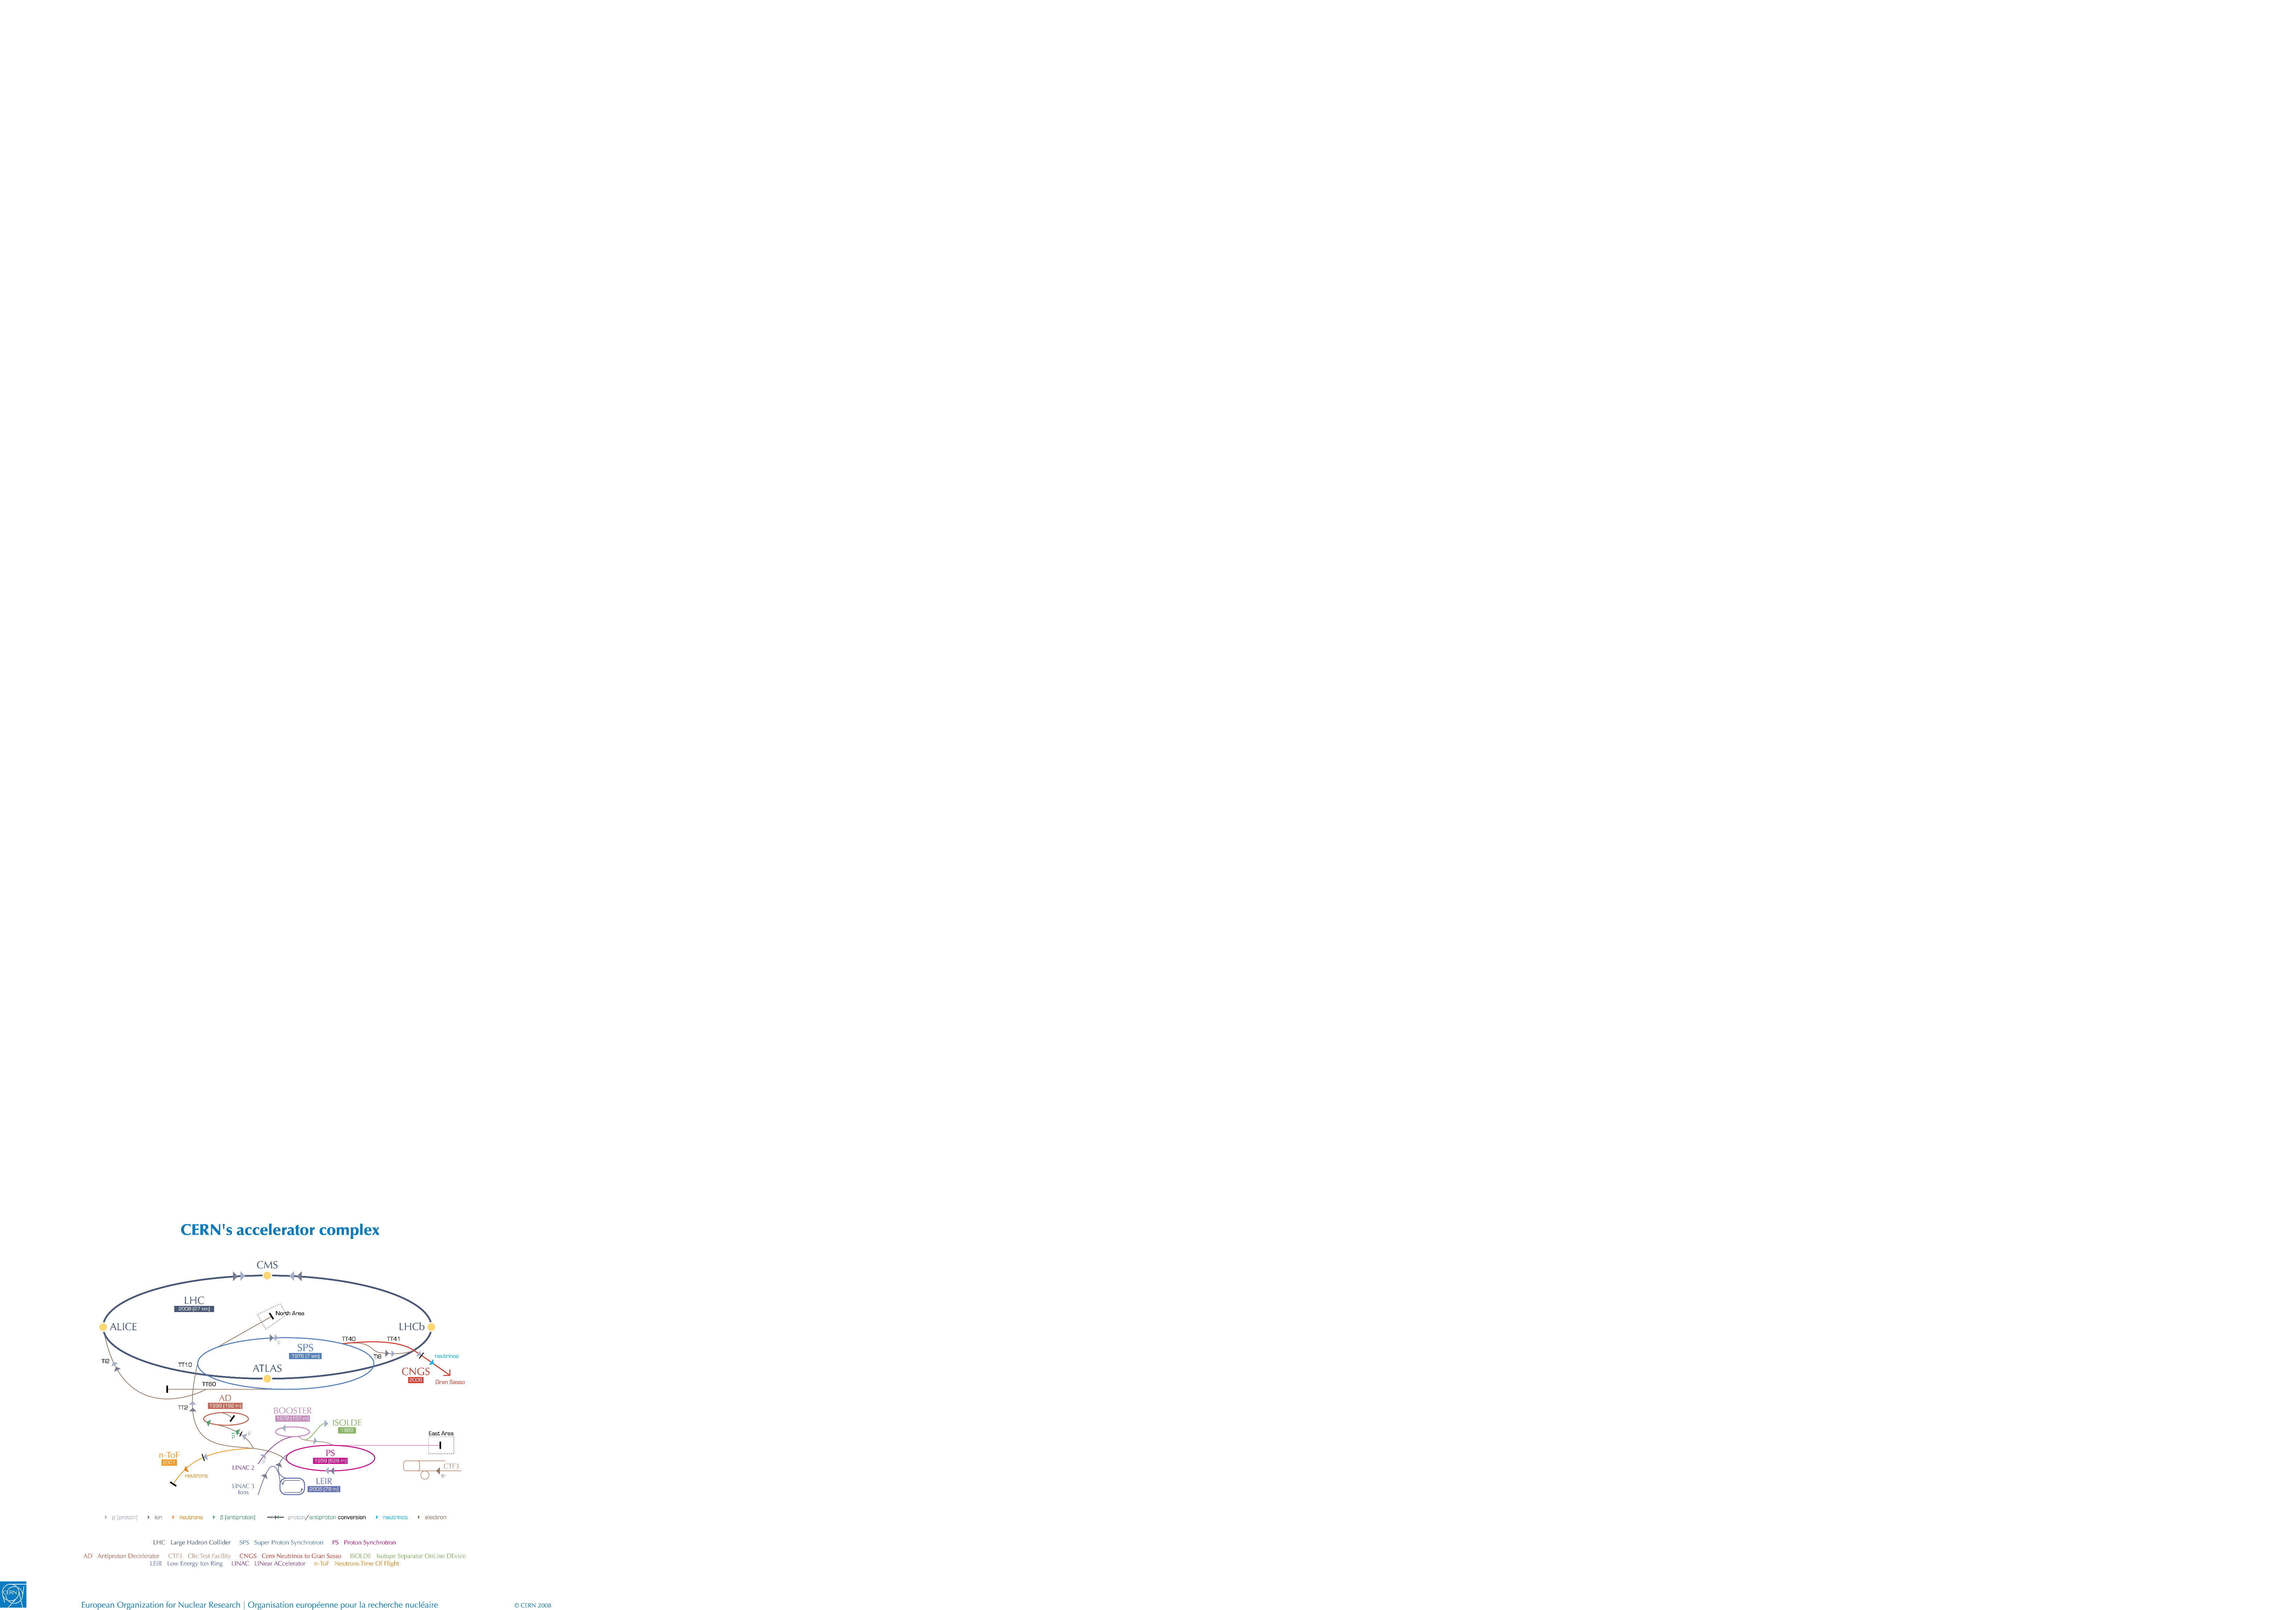
\includegraphics[width=.7\textwidth]{lhc-accelerator}
  \caption[The CERN accelerator complex]{The CERN accelerator
    complex~\cite{LHC-acc-fig}.}%
  \label{fig:lhc-acc}
\end{figure}

The Lorentz force is fundamental to the LHC's accelerator technologies and
detectors. Expressed as
\begin{equation}
  \label{eq:lorentz}
  \vec{F} = q(\vec{E} + \vec{v} \times \vec{B}),
\end{equation}
it is clear that the force due to an electric field $\vec{E}$ on a particle with
charge $q$ acts in the direction of the velocity of the field whereas the force
due to a magnetic field $\vec{B}$ acts perpendicular to both the field and the
velocity of the particle $\vec{v}$. It is therefore clear that an electric field
may be used to accelerate and give energy to a charged particle whereas a
magnetic field will alter the trajectory of a particle whilst keeping its energy
constant.

The LHC is a synchrotron, an accelerator that uses magnets in a dipole
configuration, such as in figure~\ref{fig:dipole}, to bend the path of charged
particles into conformity with its circular shape. It is apparent from studying
the figure that counter-rotating beams of same sign charged particles will
require two sets of dipole magnets in order to rotate in opposite directions
around the same ring. This is one disadvantage of a proton-proton collider with
respect to a proton-anti-proton collider such as the Tevatron~\cite{tevatron-01}
which can use the same magnets for both beams. On the other hand, the
proton-proton collider is able to separate the beams after they have been
brought together to collide with a single dipole. The bending magnets of a
synchrotron are designed to ramp up their magnetic field in synchronoisation
with the kinetic energy of the accelerated particles, allowing higher energies
to be achieved before the beam is lost. The LHC can accelerate each beam to an
energy of 6.5~TeV leading to collisions with a centre of mass energy of
$\sqrt{s} = 13 $~TeV, although the design energy of the LHC is $\sqrt{s} = 14
$~TeV. The Tevatron held the previous record for centre of mass energy of
collisions of $\sqrt{s} = 2 $~TeV. The LHC has 1232 dipole magnets~\cite{LHC-dr}
which are made of copper-clad niobium-titanium cables, a superconducting
material whose electrical resistance falls to zero below $10$~K. In order to
maintain super-conductivity a cryogenic system using liquid helium is employed
to cool the magnets. The higher the velocity of a charged particle, and the
tighter the desired bending radius, the larger the magnetic field required to
perform the bending. The large size of the LHC and the choice of superconducting
magnet technologies are both informed by the aim to accelerate protons to the
highest energy, and therefore velocity, possible.
\begin{figure}[ht]
  \centering
  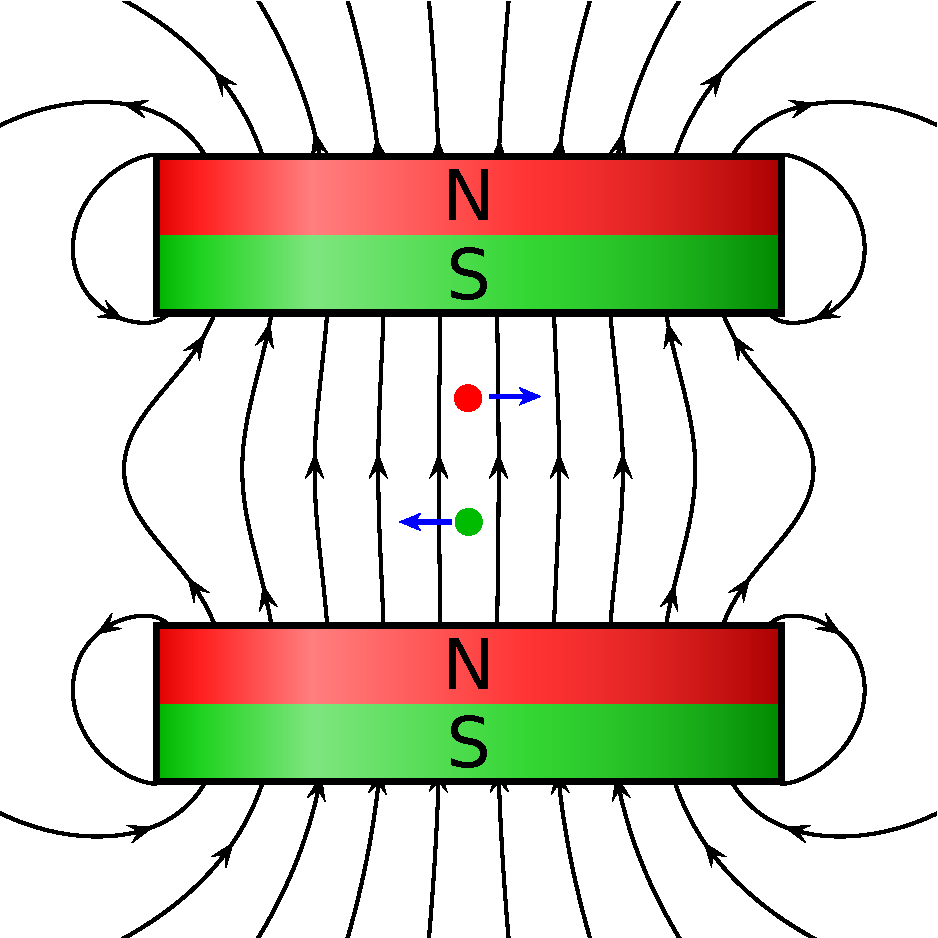
\includegraphics[trim={1cm 1cm 1cm 1cm}, clip, width=.5\textwidth]{uniform_gap}
  \caption[Magnets in a dipole configuration.]{A representation of a pair of
    idealised cylindrical magnets in a dipole configuration. Two positively
    charged particles are shown as circles, the red particle is traveling out of
    the page, the green particle is traveling into the page. The forces
    experienced by each particle due to the magnetic field are shown as blue
    arrows.}
  \label{fig:dipole}
\end{figure}


The force which accelerates the particles is provided by radio-frequency
cavities such as in figure~\ref{fig:rf-cavity}, of which the LHC has
16~\cite{LHC-dr} The electric field in the radio-frequency cavity forms a
standing wave, the separation between bunches of particles to be accelerated
must be matched to the frequency of this wave. Protons in the LHC are
accelerated in bunches and in vacuum, this to increase the likelihood of
collisions and mitigate loss of energy and scattering effects due to
interactions with air molecules. These two factors lead to the occurrence of
space charge which causes an increase in the emittance of the beam, where the
emittance is defined as the total area that the beam occupies in its beam-pipe.
The greater the energy of the particles the more they can overcome increase in
emittance due to space charge. Increased emittance is especially problematic in
circular accelerators where periodic effects can quickly lead to the loss of
beam. For these reasons it would be very challenging to accelerate protons from
rest in a synchrotron, the starting point for the protons of the LHC is
therefore a linear accelerator called Linac2~\cite{linac2} which is used to
overcome space charge effects before the protons move on to a series of
synchrotrons as seen in figure~\ref{fig:
  lhc-acc}.
\begin{figure}[ht]
  \centering
  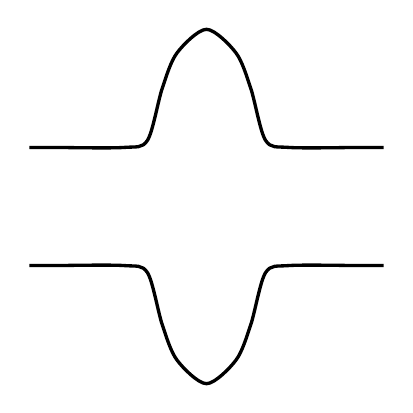
\begin{tikzpicture}[scale=1.5]
    \draw [very thick] plot [smooth] coordinates {(0,1) (0.2, 1) (0.8, 1) (1, 1.06)
      (1.125, 1.5) (1.25, 1.8) (1.5, 2) (1.75, 1.8) (1.875, 1.5) (2, 1.06) (2.2, 1)
      (2.8, 1) (3, 1)};

    \draw [very thick] plot [smooth] coordinates {(0,0) (0.2, 0) (0.8, 0) (1, -0.06)
      (1.125, -0.5) (1.25, -0.8) (1.5, -1) (1.75, -0.8) (1.875, -0.5) (2, -0.06) (2.2, 0)
      (2.8, 0) (3, 0)};
    
  \end{tikzpicture}
  \caption[A radio-frequency cavity.]{A representation of a radio-frequency
    cavity where the electric field lines are shown in black.}
  \label{fig:rf-cavity}
\end{figure}


Even a beam with its emittance under control would still be lost from the
accelerator if only dipole magnets were used to control its path. Magnets in a
quadrupole configuration as in figure~\ref{fig:quadrupole} are used to focus the
beam and keep it in the beam-pipe. The quadrupoles behave such that particles
feel a force that increases with the distance from the centre of the beam
leading to simple harmonic motion of individual particles in a bunch. The LHC
has a series of 24 quarupole magnets each for focusing in the horizontal and vertical
directions~\cite{LHC-dr} as well as higher multiplicity configurations;
sextupole, octupole, decapole and dodecapole which are used to correct
imperfections in the fields of other magnets.
\begin{figure}[h]
  \centering
  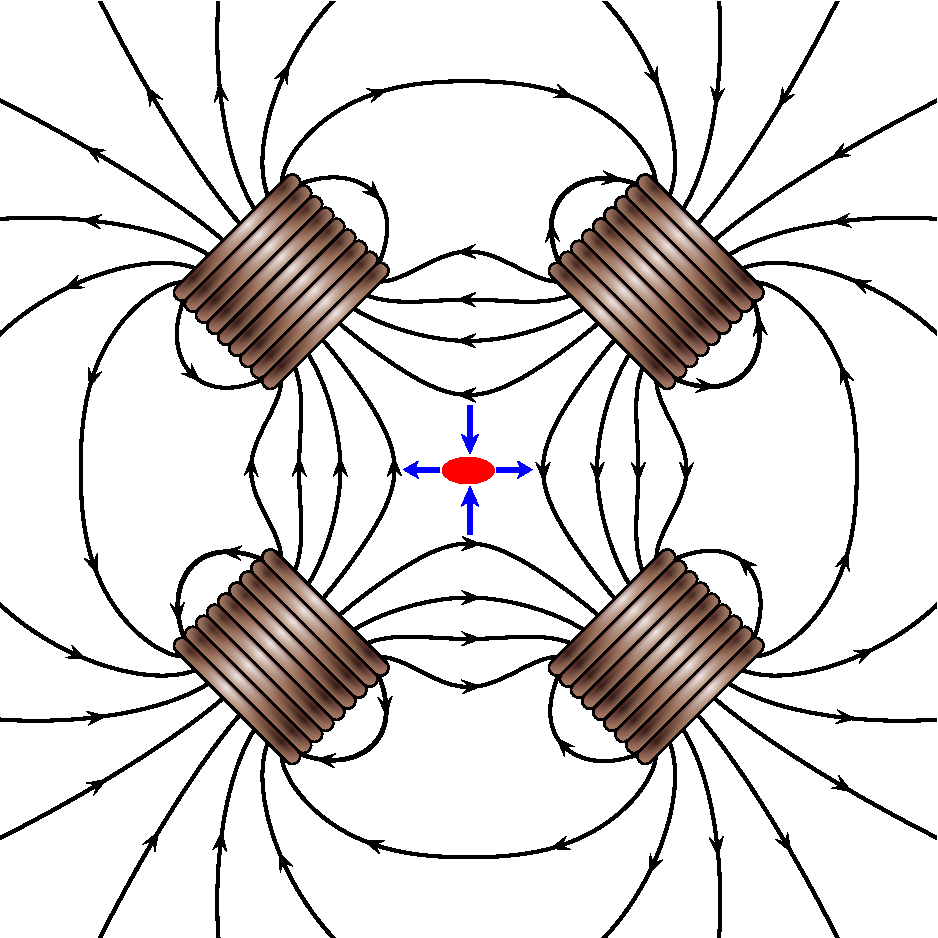
\includegraphics[width=.7\textwidth]{quarupole_with_beamspot}
  \caption{Representation of an idealised set of coil magnets in a quadrupole
    configuration with a proton beamspot shown as a red ellipse. The proton beam
    is drawn coming out of the page (\emph{watch out!}), magnetic field lines
    are drawn in black and the forces acting on each bunch of protons are drawn
    as blue arrows.}
  \label{fig:quadrupole}
\end{figure}

% The LHC receives protons that have already been accelerated somewhat by the
% Super Proton Synchrotron (SPS), another of the accelerators at the CERN
% accelerator complex shown in figure~\ref{fig:lhc-acc}. The circular design of
% both the LHC and SPS allows protons to be accelerated many times around their
% respective rings until their velocity is fast enough for a high energy
% collision. The highest energy collisions achieved take place at a centre of mass
% energy of $\sqrt{s} = 13 $~TeV, although the design energy of the LHC is
% $\sqrt{s} = 14 $~TeV. Despite having not yet reached its design energy the LHC
% collides particles with the highest energy of any particle collider in history
% and is currently alone at the energy frontier of modern physics. At the time of
% writing the LHC is in it's second long shutdown during which maintenance and
% upgrades to the LHC and the particle detectors located around its ring take
% place. The LHC has completed two runs data taking from collisions, Run 1 took
% place from 2009 to 2013, followed  by Run 2
% between 2015 and 2018. The period between runs is known as long shutdown 1 (LS1), and
% was used to perform maintenance and upgrades. Many analyses from Run 1 have been
% published including, most notably the discovery of the Higgs
% boson~\cite{DiscoHiggsATLAS, DiscoHiggsCMS}. Some Run 2 analyses have also
% published results a highlight of which is LHCb's discovery of charge parity
% violation in charm decays~\cite{cp-charm}. Despite these impactful results there
% are many more results expected from the LHC experiments as data continues to be
% analysed.

The statistical nature of particle physics analyses means that larger datasets
(more recorded collisions) increase the sensitivity of searches and
measurements. Constraints on the number of years the LHC is able to run for mean
that the best way to record more collisions is to collide more particles per
second. A quantity known as the luminosity is often used to describe how much
data is available for an analysis, it is written as
\begin{equation}
  \label{eq:luminosity}
  L = \frac{1}{\sigma}\frac{dN}{dt},
\end{equation}
where $\sigma$ is the cross-section, a volume within which particles must pass
by one another in order to interact, and $N$ is the number of events recorded in
a period of time $t$. For luminosity at the LHC N can be expressed as
\begin{equation}
  \label{eq:lhc-lumi}
  N = n_{bp}n_{1}n_{2}\nu_{r},
\end{equation}
where $n_{bp}$ is the number of colliding bunch pairs, $n_{1}$ and $n_{2}$ are
the number of protons in each beam and $\nu_r$ is the frequency with which the
beams rotate around the LHC's circumference. The number of particles in the
beams is limited by space charge. The number of bunches is limited by the
frequency that the radio-frequency cavities can operate at. The revolution
frequency is limited by the strength of the dipole magnets and the circumference
of the accelerator ring. Increasing luminosity by reducing the cross-section
amounts to reducing the beam widths which is limited by the emittance of the
beam. The LHC has already exceeded it's design luminosity providing physicists
with more data to analyse than expected and plans are well underway for the
upgrade to a High-Luminosity LHC (HL-LHC)~\cite{hilumi-tdr}.

\section{The ATLAS Detector}%
\label{sec:atlas}

The ATLAS detector~\cite{ATLAS} resides at a location on the LHC ring called
Point 1, its full name is A Toroidal LHC ApparatuS. A diagram of the detector is
shown in figure~\ref{fig:ATLAS-det}. ATLAS is considered to be a general purpose
particle detector and has a wide physics program including: Higgs boson physics,
top quark physics, searches for Supersymmetry and exotic states, probes of CP
violation in b-quarks and light states and heavy ion physics. The detector
itself is very large in size, spanning a width of 25~m and a length of 44~m and
weighs 7000~tonnes which is comparable to the weight of the wrought iron content
of the Eiffel tower~\cite{Eiffel-weight}.
\begin{figure}[h]
  \centering
  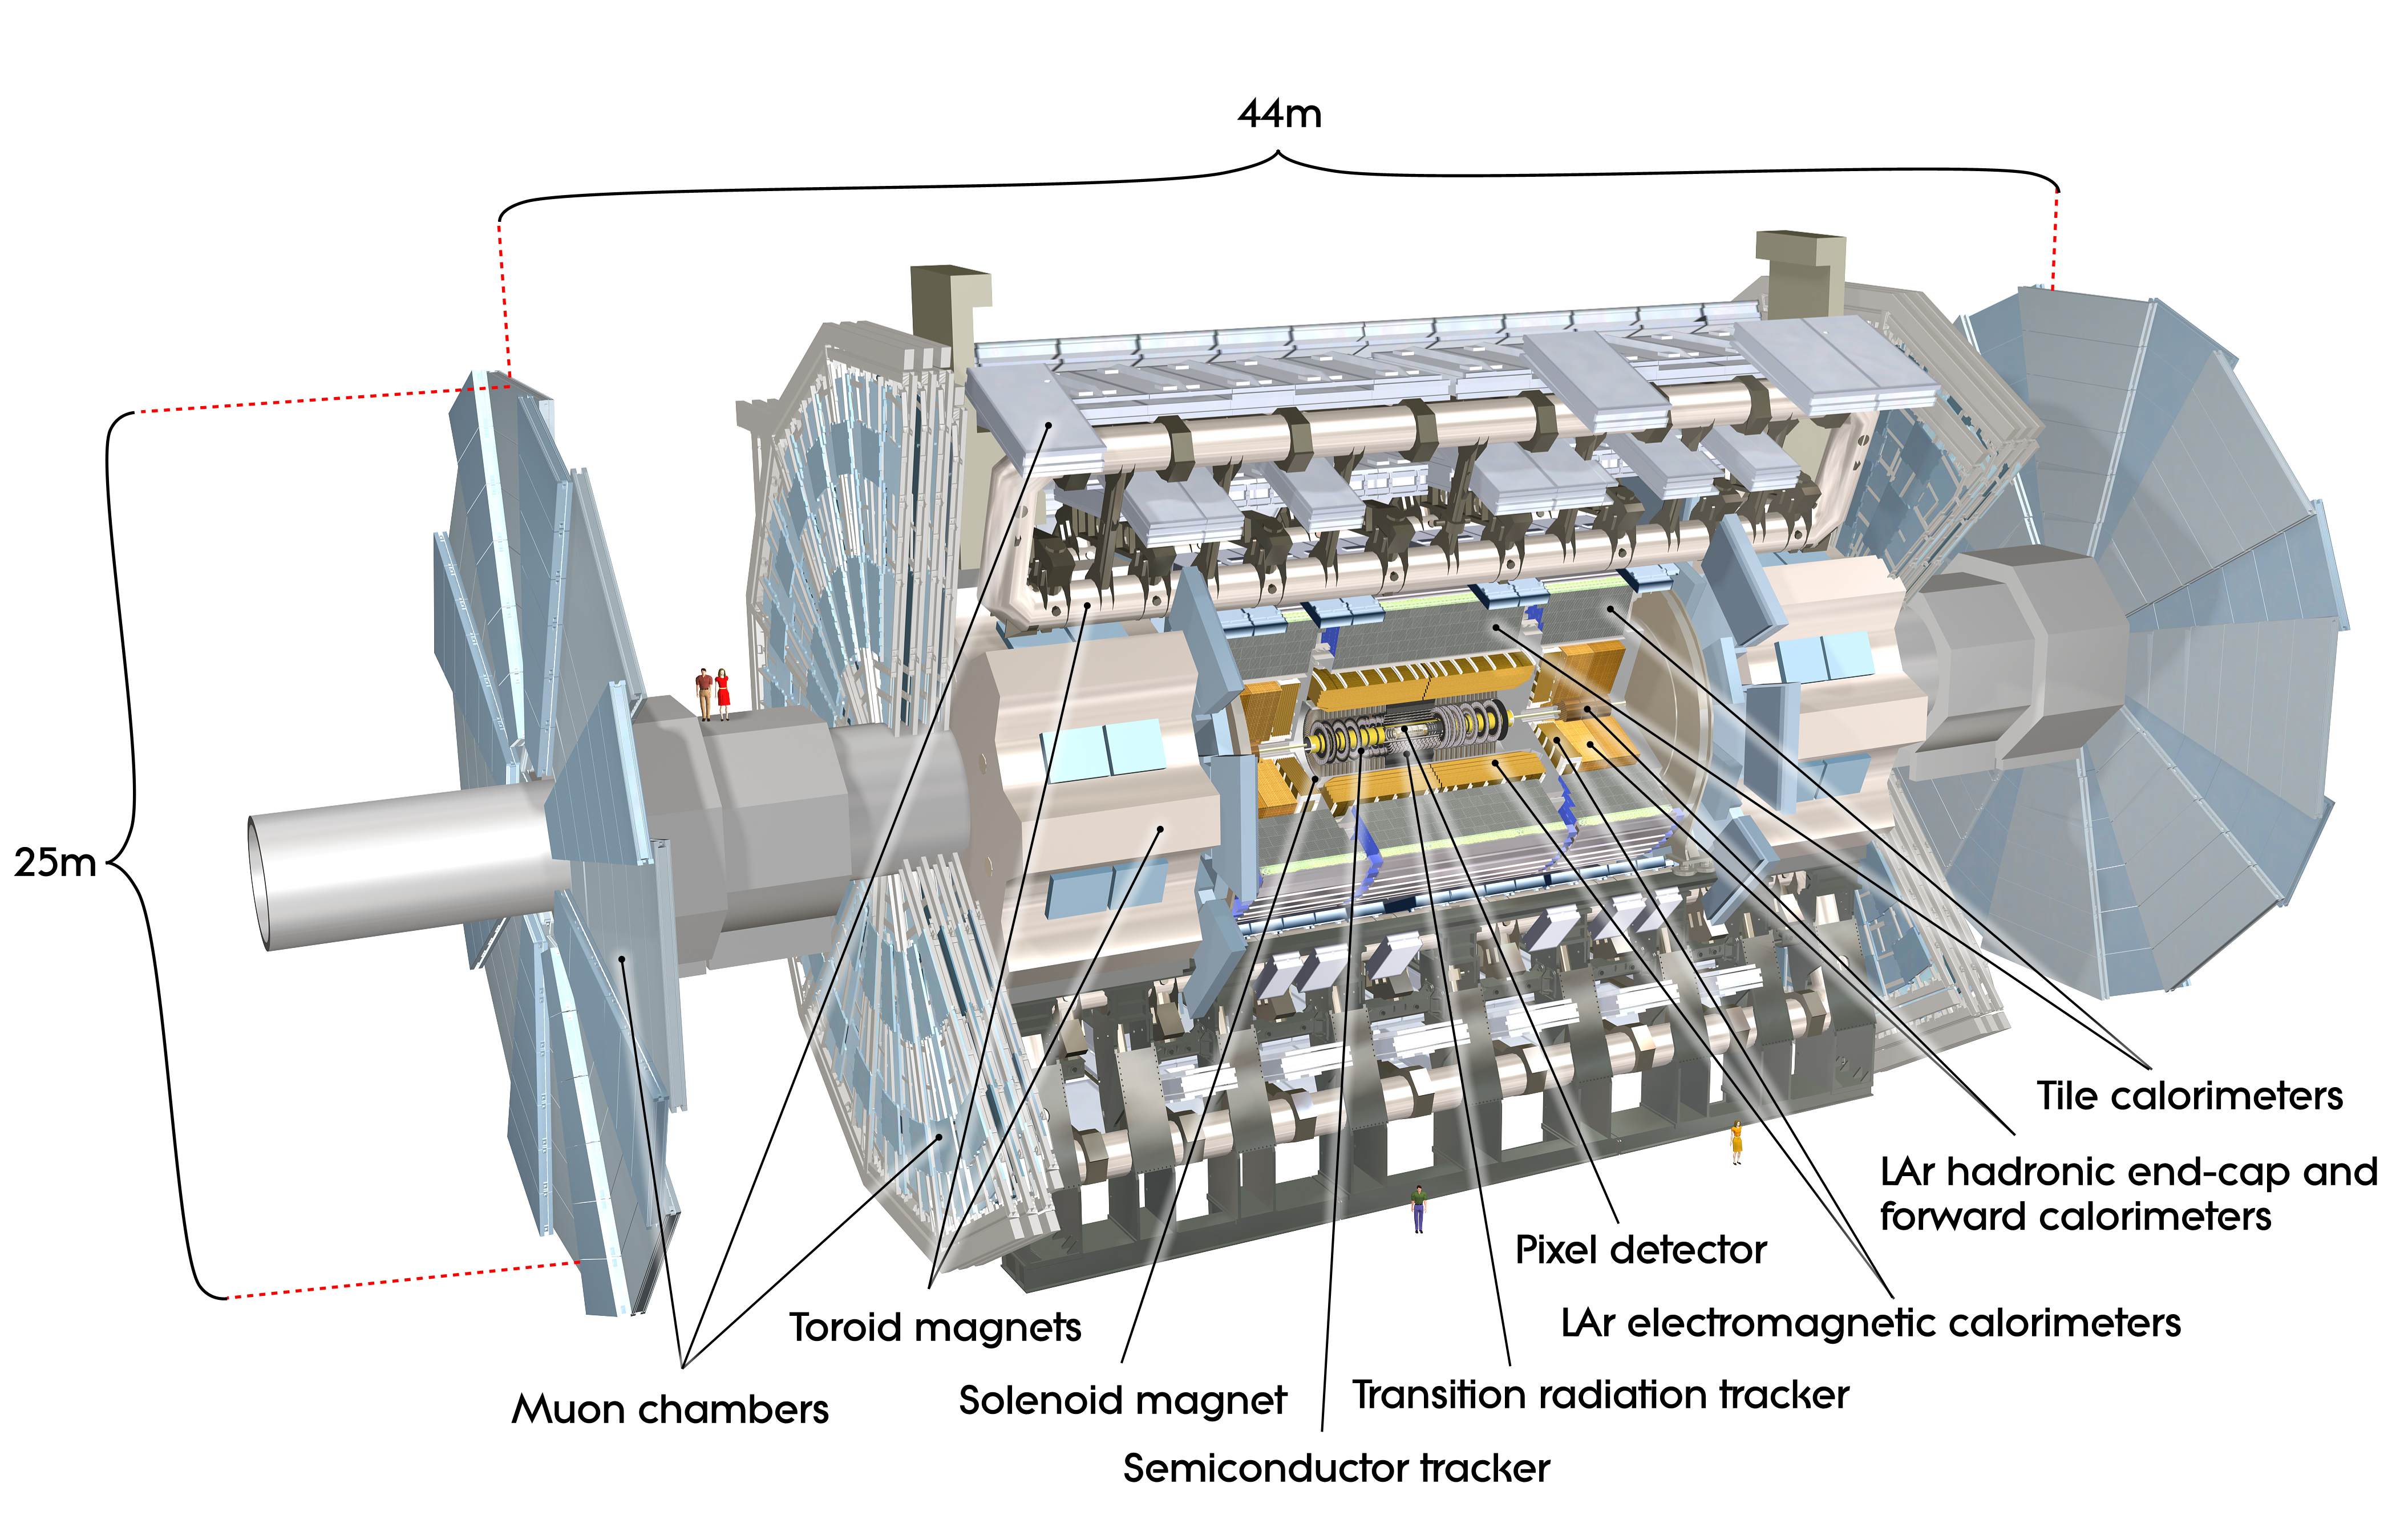
\includegraphics[width=.7\textwidth]{ATLAS-detector}
  \caption[The ATLAS Detector]{Computer generated image of the whole ATLAS
    detector with the major sub detectors labeled~\cite{ATLAS-det-fig}.}%
  \label{fig:ATLAS-det}
\end{figure}


Due to the composite nature of the proton, the decay products of collisions are
extremely numerous. Additionally when two bunches of protons cross there is the
chance that more than one hard scattering event occurs and softer glancing
collisions are also a possibility. The number of hard scattering events in a
given bunch crossing is known as the pile-up of the collision and is often
denoted with the symbol $\mu$. As can be seen by inspecting
equations~\ref{eq:lhc-lumi}~and~\ref{eq:luminosity} increasing the luminosity
will often cause a higher pile-up environment in the detector. The variety of
decay products of each collision necessitate the use of specialised
sub-detectors in order to accurately measure the output of collisions. There are
dedicated sub-systems in ATLAS with the purpose of measuring properties of
specific classes of particles. Ultimately in all cases a digital electrical
signal is the desired output of a sub-detector which usually originates as an
analogue signal. It is interesting to note that despite the many charges that
are associated with the forces of nature discussed in chapter~\ref{sec:theory}
the only one that we can directly measure is electric charge.

The ATLAS sub-systems are located in either the barrel of the detector or one of
the end-caps. These two areas have a different geometry, and due to their
relative positions with respect to the beam-pipe are exposed to different
amounts of radiation, so the design of a sub-system in the barrel will differ
from that of a sub-system measuring the same quantities in the end-cap. The
details that follow are based on the ATLAS technical design report
volumes~\cite{ATLAS-TDR-01, ATLAS-TDR-02} unless another citation is present.
Before detailing individual components it is important to detail certain
properties of the detector relevant to all sub-systems.  The coordinate system
used to describe the ATLAS detector is known as right-handed. Three orthogonal
axes $(x, y, z)$ are used to describe the 3D space of the detector. The x-axis
points towards the centre of the LHC ring, the y-axis points upwards and the
z-axis points along the LHC beam pipe y-axis. The three axes meet at the
interaction point which is the nominal position where bunches cross, located in
the centre of the detector. Cylindrical coordinates $(r, \phi)$ are also often
used to describe the physical features of the detector and phenomena caused by
interactions in the detector that shall be referred to as analysis objects.
Their definitions are that $\phi$ is the azimuthal angle in the x-y plane
(transverse) around the beam pipe and $r$ is the distance from the interaction
point. A relativistic invariant analogy to the zenith angle of an object
measured from the z-axis is pseudo-rapidity $\eta = - \ln(\tan(\theta / 2))$
where $\theta$ is the ordinary zenith angle measured from the same axis.

By inspecting equation~\ref{eq:lorentz} it is clear that neutral particles for
which $q=0$ do not experience the Lorentz force. However for charged particles,
as previously discussed, a magnetic field alters the trajectory of the particle
whilst preserving its energy. A large portion of the ATLAS detector is immersed
in magnetic fields created by the magnet systems, and so this deflection
phenomenon is present and exploited when making measurements of charged
particles. There are four magnet systems in ATLAS the solenoid, the barrel
toroid, and two end-cap toroids. The solenoid surrounds the inner detector
whilst the toroid systems surround the muon chambers.
Figure~\ref{fig:ATLAS-magnets} shows a heat map of the magnetic field strengths
within ATLAS, the image is from an article detailing the superconducting magnet
system~\cite{ATLAS-magnets}. The magnet systems store a total energy of 1.6~GJ
and produce fields of a combined volume of approximately $12\times 10^4$~m$^3$.
\begin{figure}[h]
  \centering
  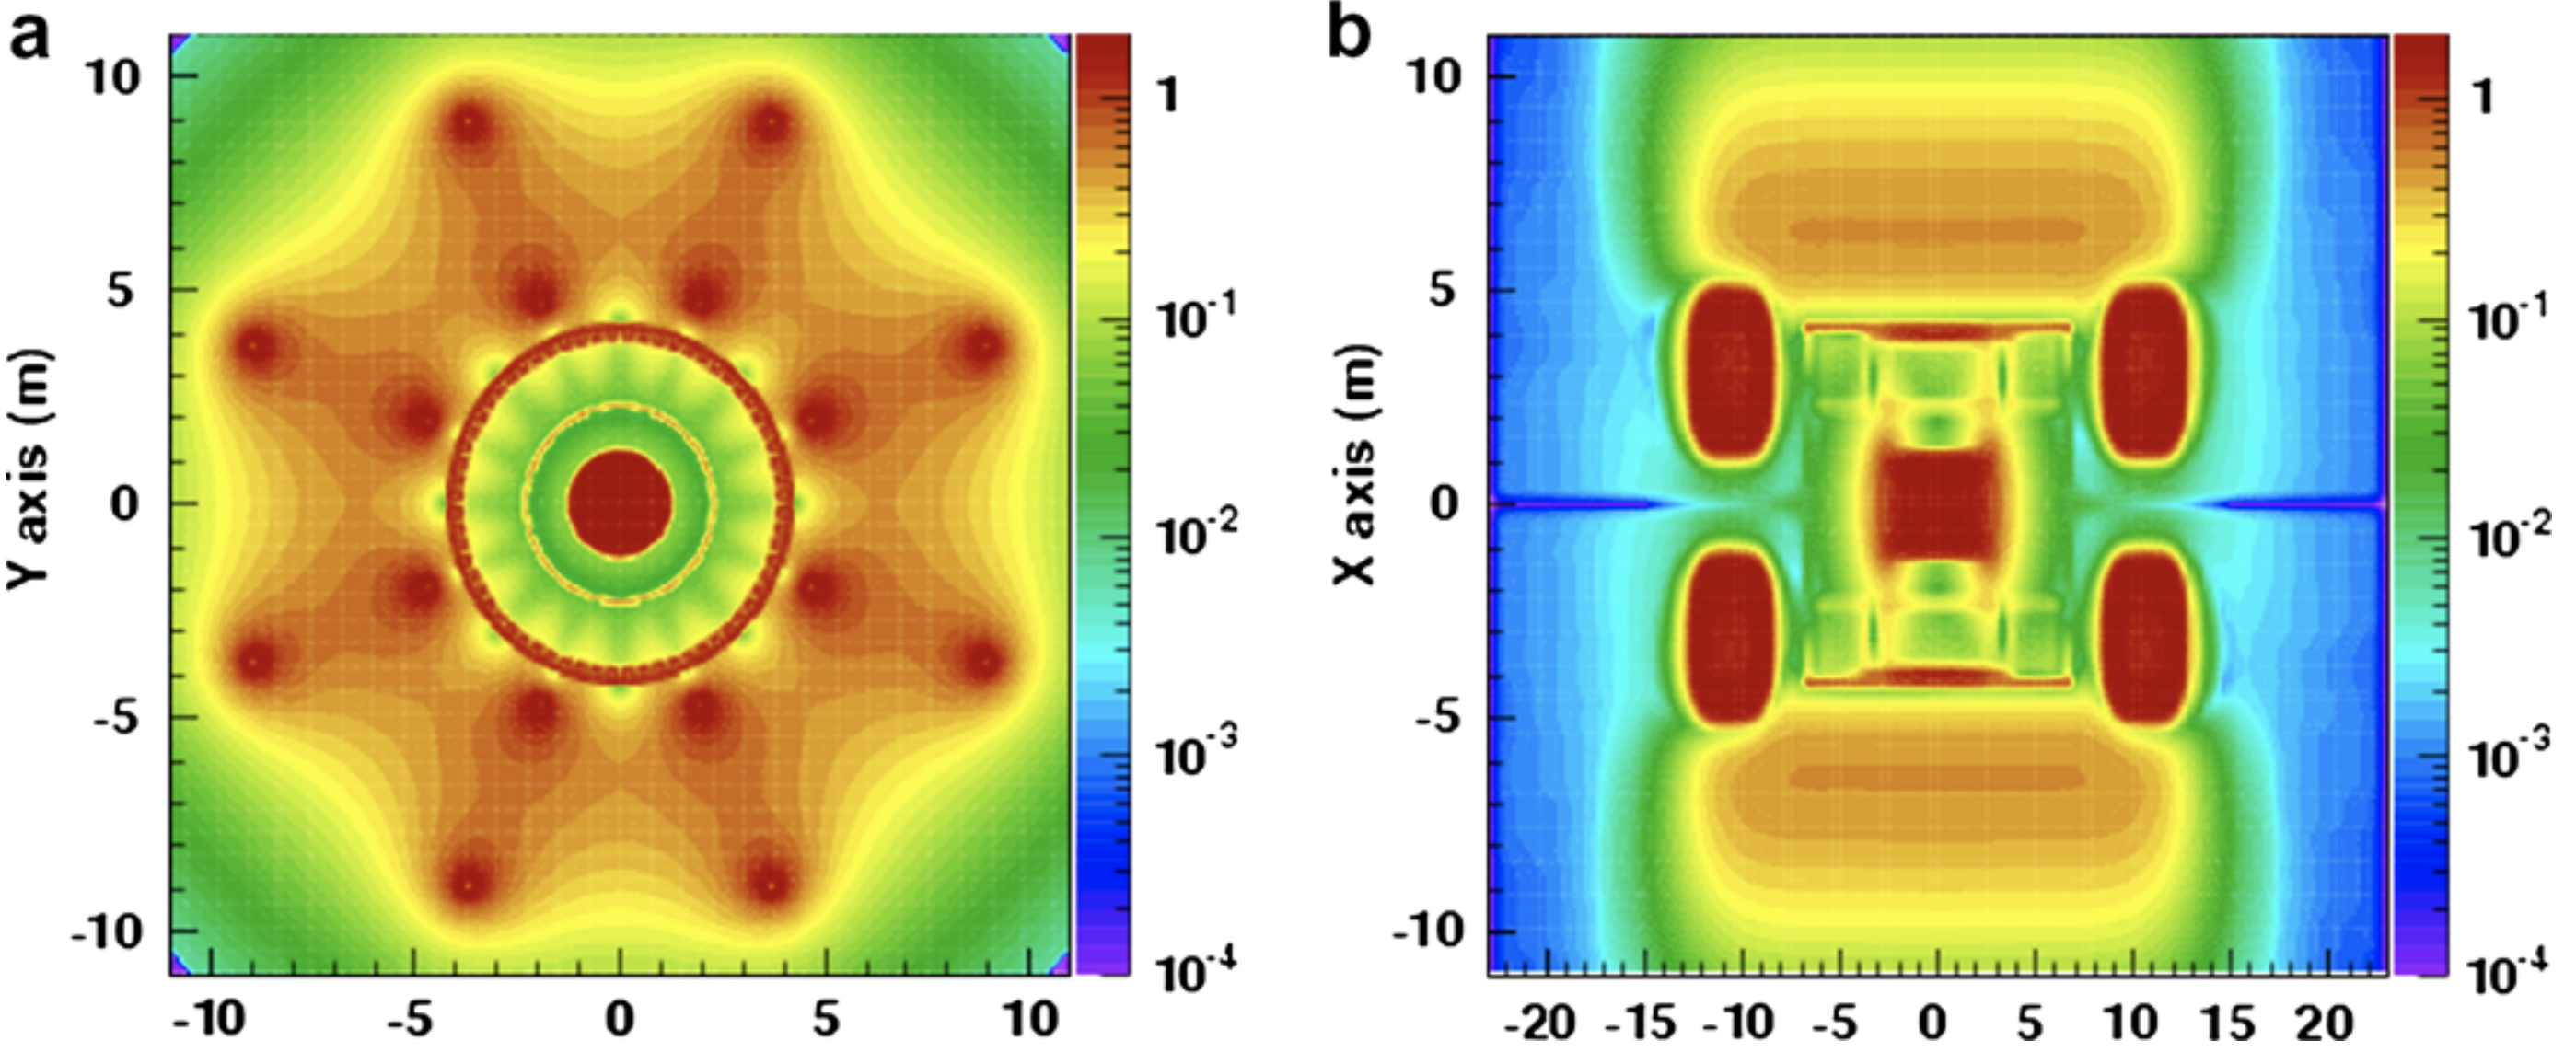
\includegraphics[width=.7\textwidth]{ATLAS-magnet}
  \caption[ATLAS magnetic field]{ATLAS magnetic field profile, showing a
    transverse cross-section in the centre of the detector (a), and a
    longitudinal section (b)~\cite{ATLAS-magnets}.}%
  \label{fig:ATLAS-magnets}
\end{figure}

\subsection{Tracking: The Inner Detector}%
\label{sec:id}

The Inner Detector (ID) is comprised of a number of different tracking detector
sub-systems; the pixel detectors, the semiconductor
tracker (SCT) and a transition radiation tracker (TRT) as seen in
figure~\ref{fig:ATLAS-inner-det}. It covers a volume corresponding with the
total $\phi$ angle. The pixel detectors and SCT cover the range $|\eta|~<~2.5$
and the TRT covers $|\eta|~<~2.0$. The job of the ID is to track the propagation
of charged particles through the detector. This is achieved by measuring a
sequence of hits for each charged particle that propagates through its volume.
The sequence of hits describing the trajectory of a given charged particle must
be disentangled from other hits in the detector, track-finding algorithms are
applied to this end. Using these tracks we can measure; the direction of the
particle, the sign of the electric charge of the particle, the rate of energy
loss of the particle with respect to its distance traveled and by constructing
the sagitta the transverse momentum of the particle (denoted $p_T$). An example
construction of the sagitta is shown in figure~\ref{fig:sagita} and its relation
to $p_T$ is
\begin{equation}
  \label{eq:sagitta}
  S = \frac{qL^{2}B}{8p_{T}},
\end{equation}
where $L$ is the distance between the first and last hits in the track, $q$ is
the charge of the particle, and $B$ is the strength of the magnetic field, in
this case the field produced by the solenoid magnet system. The system is made
of a single layer coil with an inner diameter of 2.46~m  and produces 2~T field
in the axial direction with respect to the beam-pipe. Using multiple tracks
interaction vertices can also be reconstructed, the vertex which comes from the
highest energy collision in a given event is known as the primary vertex.
Vertices coming from pile-up and glancing collisions of partons also need to be
reconstructed in order to separate detector response due to these collisions
from that of the primary vertex. So-called impact parameters $d_0$ and $z_0$ are
used to identify secondary and pile-up vertices, their construction is shown in
figure~\ref{fig:impact-params}. These parameters are also used to perform
identification of particles within the detector such as $b-$quarks and $\tau$s.
Tracks are also used to calculate the calorimeter impact point and in general
match activity in outer regions of the detector to an interaction vertex.
\begin{figure}[h]
  \centering
  \includegraphics[width=.7\textwidth]{Inner-detector}
  \caption[ATLAS inner detector]{Computer generated image of the ATLAS inner
    detector~\cite{ATLAS-inner-det}.}%
  \label{fig:ATLAS-inner-det}
\end{figure}

With the exception of the TRT the tracking sub-systems are silicon based
detectors. The silicon detection medium acts as a reverse bias diode. Charged
particles incident on the silicon cause ionisation in the depletion layer. The
products of this ionisation are electons and holes (excess pockets of positive
charge in the silicon) which produce a signal that must be handled by a
read-out system. The signal is referred to as the charge collected.
Application-specific integrated circuits (ASICs) are used to readout the signal
performing the analogue to digital conversion. The combination of the detection
medium, readout system and the printed circuit board (PCB) on which they are
joined is referred to as a module.

\subsubsection{Pixel Detectors}

There are four layers of pixel detectors that are the closest components of the
ID to the beam-pipe. Pixel detectors are silicon detectors where the diodes are
approximately square in shape, giving the benefit of being able to resolve hits
in two directions. The design originally had three layers, each 250~$\mu$m
thick with 50~$\mu$m by 250~$\mu$m pixels, of oxygen doped n-type silicon
crystals. During LS1 a fourth layer, closest to the beam-pipe (which was also
replaced for a smaller radius version) was added. This layer is known as the
insertable B-layer (IBL)~\cite{IBL-TDR}, the motivation for its addition was to
counteract degradation of original performance of the ID due to irreversible
damage by radiation. As well as the inclusion of the IBL, performance degradation
is mitigated by increasing the bias voltage across the pixels from 100~V (their
starting voltage) to up to 600~V. Additionally the IBL being closer to the
beam-pipe allows for interaction vertices to be measured more precisely. The
need for better reconstruction of vertices is motivated by their role in the
performance of algorithms that classify jets of activity in the detector that
are initiated by B-hadrons, this is where the IBL gets its name. There are no
pixel detectors in the end-caps. Each pixel is small in size which mean many can
fit on one module, all requiring their own conductor for readout. The solution
to this challenge is to use a complex process known as bump bonding, which is
both expensive and time consuming.

\subsubsection{Semiconductor Tracker}

Next closest to the beam-pipe is the SCT whose modules have long thin strip
shaped diodes. The strips provide high resolution in only a single direction. In
contrast to the n-type silicon of the pixels, the strips are made from p-in-n
type silicon. Each SCT module is comprised of two back to back wafers such that
the orientation of the strips are offset by a small angle in order to improve
coverage. Each strip is covered in a metalised layer, the strips are separated
by a distance of 80~$\mu$m. A rather old and dirty SCT module left over from the
quality control testing stage of production that took place at Queen Mary
University of London can be seen in figure~\ref{fig:strip-module}. As can be
seen in the figure the SCT modules are wire bonded to their ASICs which is
cheaper and faster than the bump bonding used on the pixel modules.
\begin{figure}[h]
  \centering
  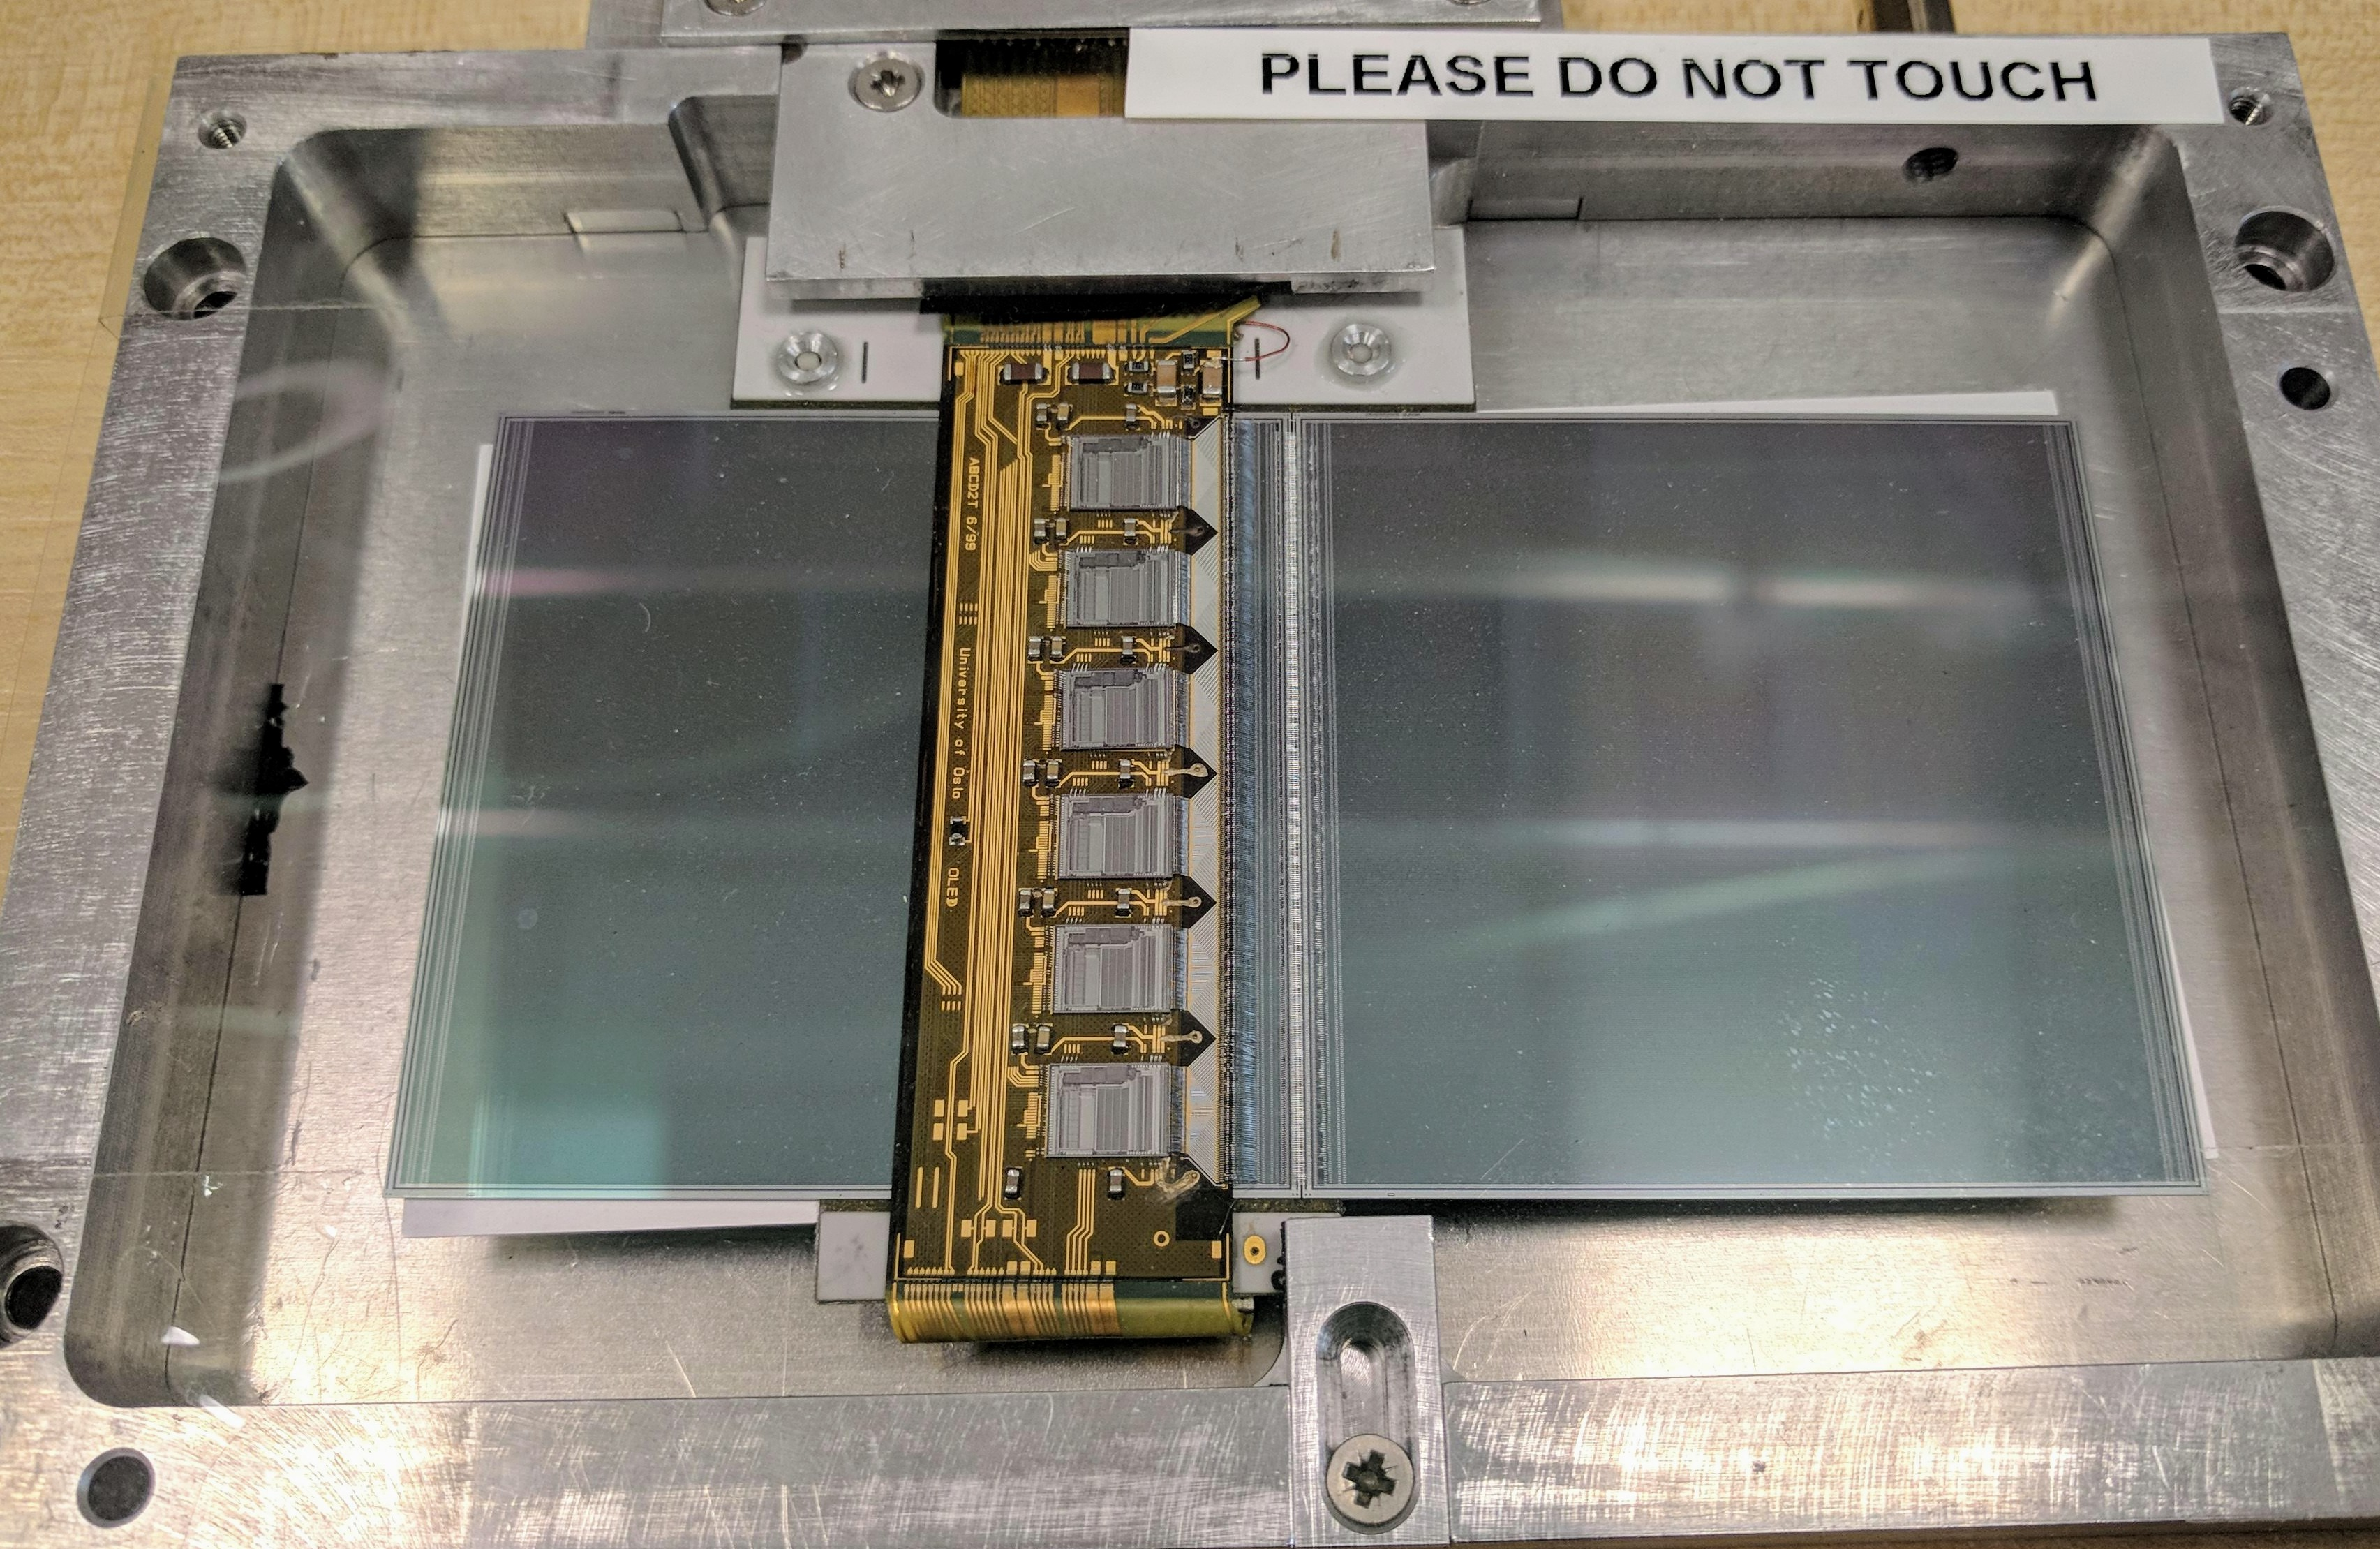
\includegraphics[width=.7\textwidth]{sct-module}
  \caption[ATLAS long strip module]{An image of an SCT long strip module
    mounted in a rig for testing at Queen Mary Univesity of London.}
  \label{fig:strip-module}
\end{figure}
In order to calibrate the response of the strips a 100~M$\Omega$ poly-silicon
resistor is located at the end of each strip. Figure~\ref{fig:sct-close} shows an
image of the snake-like structure of a poly-silicon resistor from the end of an
SCT module.
\begin{figure}[h]
  \centering
  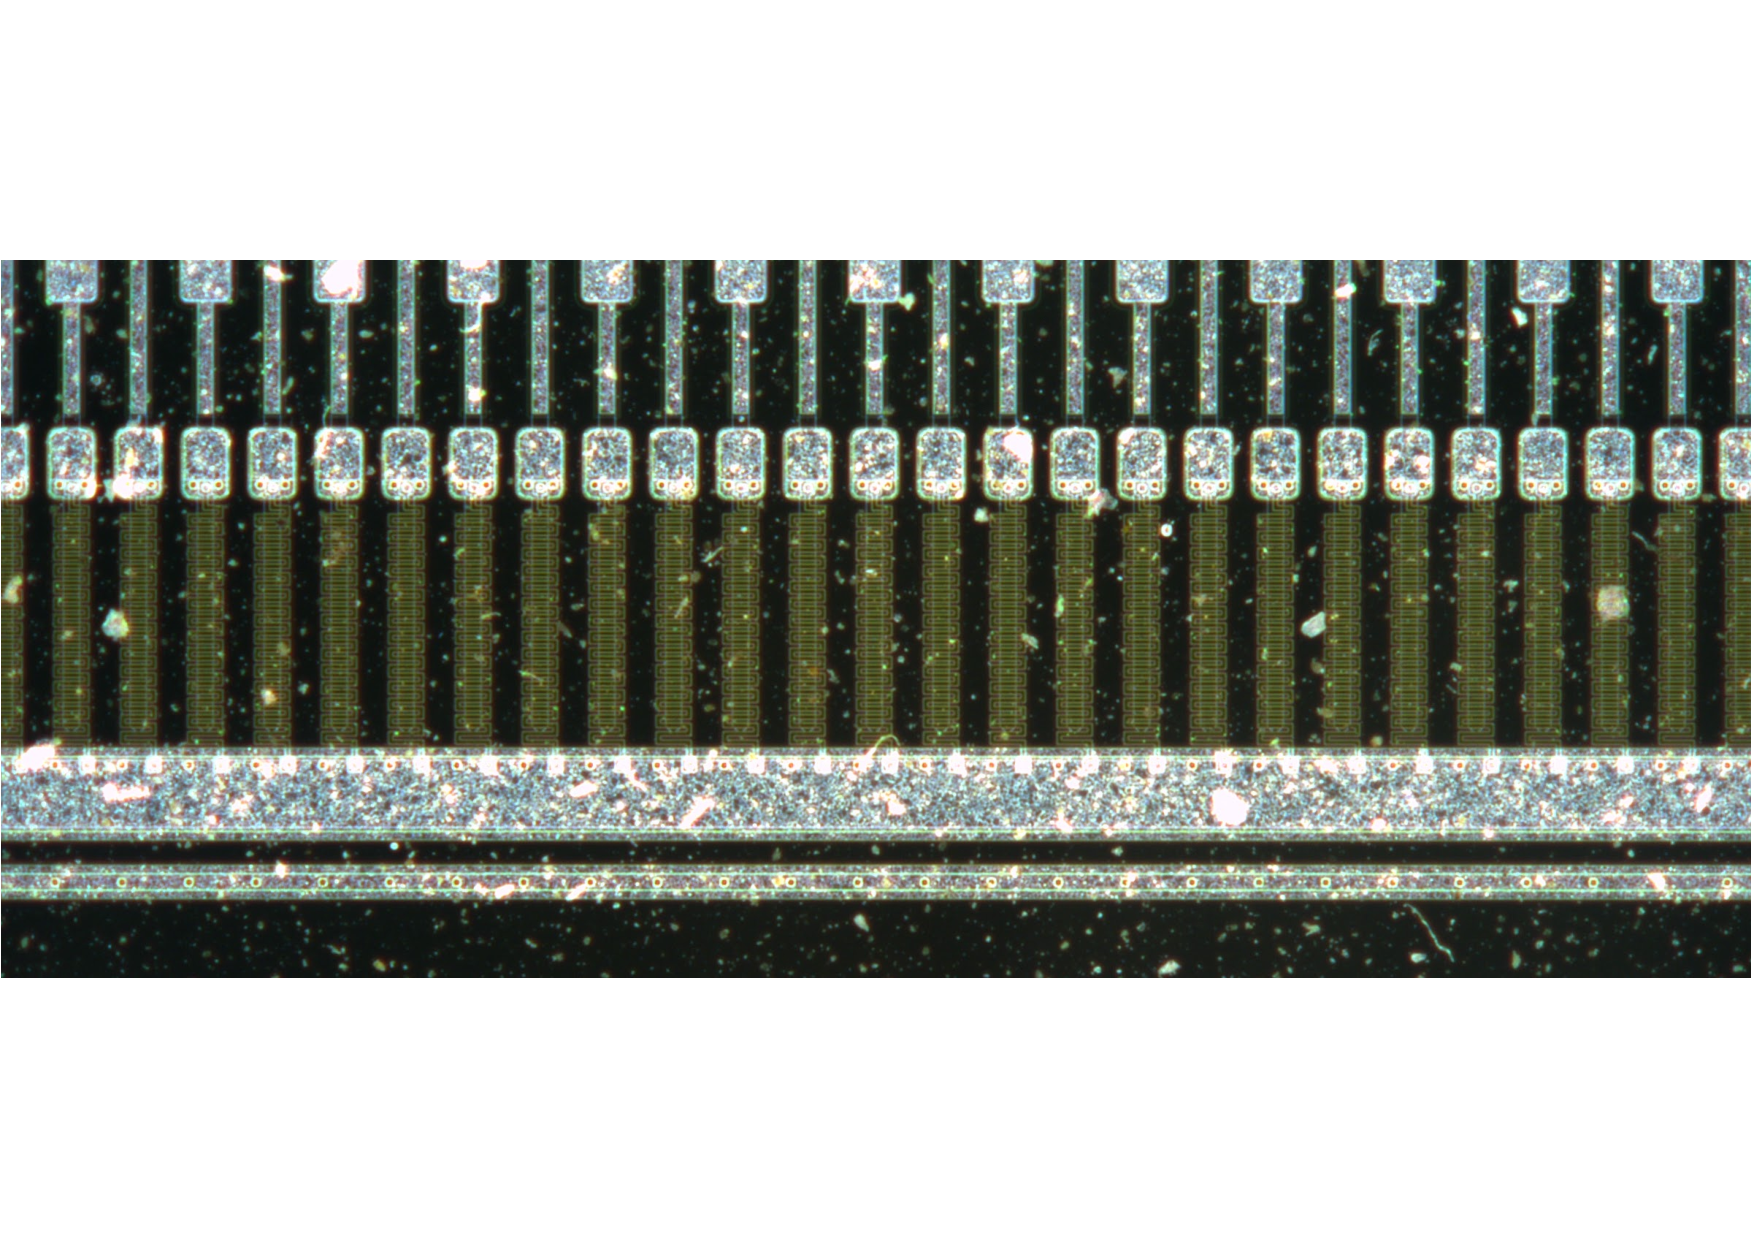
\includegraphics[width=.7\textwidth]{sct-close}
  \caption[ATLAS strip close-up]{A close up image of the end of an SCT sensor in
    which the snake-like poly-silicon reistors are visible as a yellowish
    coloured structure at the end of each strip. This image was taken with a
    high resolution automatic area scanner commissioned by the
    author~\cite{itk-scanner} in order to take full scans of strip sensors
    during the production of the ATLAS Inner Detector upgrade known as the Inner
    Tracker (ITk)~\cite{itk-tdr, itk-strips-tdr}.}
  \label{fig:sct-close}
\end{figure}
The modules come in two different designs, short strips and long
strips with the short strips forming the layer closest to the pixel detectors
and the long strips on the outside. The original operating bias voltage was
150~V but again due to radiation exposure this will raise to up to 350~V over
time as necessary. There are four layers of semiconductor trackers in the barrel
arranged so that sensors have a tilt with respect to a perfect coaxial cylinders
of approximately 11~$\degree$. This tilt increases the amount of material that
particles will travel through and is optimized to the geometry of the detector.
Similarly the end-cap modules are arranged in petal like structures, with a
number of different geometric designed based on the position within the end-cap.

\subsubsection{Transition Radiation Tracker}

The final layer of the ID is the TRT, the primary role of the TRT is to aid
electron identification by measurement of transition radiation. The TRT is
mostly made up of polyimide drift tubes with a diameter of 4~mm. The drift tubes
are filled with a gas mixture whose majority constituent is xenon. These tubes
operate with a voltage of -1530~V and are contained within a carbon fibre
support structure. The geometrics layout of the tubes is optimized for
both the barrel and end-caps.

\subsection{Calorimeters}%
\label{sec:calo}

The purpose of the calorimeters is to measure the total energy of particles that
pass through their volume, this is achievable only if the calorimeter
stops the particle completely. A desirable side effect is that they also act as
a barrier to stop particles passing through to the muon spectrometers, of course
this means necessarily that muons pass through the calorimeters. There are two
calorimeter systems in ATLAS the electromagnetic calorimeter (ECAL) and the
hadronic calorimeter (HCAL), they will be explained in the following sections.
The calorimeters are not immersed in a significant magnetic field compared to
the rest of the ATLAS as seen in the heat map of figure~\ref{fig:ATLAS-magnets}.
The geometric layout of the calorimeter systems, as well as the location of
specific components can be seen in figure~\ref{fig:ATLAS-calo}, in which the ID
can also be seen (greyed out). Information from the two calorimeters is used in
conjunction for any particles whose decay products propagate through both
volumes. Both calorimeters are split up into cells of material that are used to
determine the position of decay products in the detector.
\begin{figure}[h]
  \centering
  \includegraphics[width=.7\textwidth]{ATLAS-calo}
  \caption[ATLAS Calorimeter]{Computer Generated image of the ATLAS
    calorimeter~\cite{ATLAS-calo-fig}.}%
  \label{fig:ATLAS-calo}
\end{figure}

High energy physics calorimeters function by measuring the shower
of particles that are produced as a result of the incident particle losing its
energy Both calorimeters in ATLAS are sampling calorimeters, meaning that they
are comprised of alternating layers of absorber and detection medium. The purpose
of the absorber medium is to provide a material in which particle showers evolve
rapidly over a short distance, though they are in general not sensitive to
measuring those showers. The detection medium or active material is used to then
measure those showers.

\subsubsection{Electromagnetic Calorimeter}
The ECAL is primarily concerned with measuring the energy of electrons,
positrons and photons. Theses particles primarily interact with the
electromagnetic force and so produce electromagnetic showers when they lose
their energy. The ECAL resides closer to the interaction point that the HCAL and
has liquid argon (LAr) as it's active material. LAr is a good choice for the
calorimeter which is closer to the interaction point as it is naturally
resistant to damage by radiation. The absorber of the ECAL is lead, it is
suitable as it has a high number of nucleons ($Z$) and the radiation
length\footnote{The radiation length $X_{0}$ is the thickness of material that
  reduces the energy of a particle by a factor of $e$ the natural number.} of a
given shower is inversely proportional to $Z^2$. An applied electric field
causes ions produced in the EM shower to drift in such a way that the signal
induced is proportional to the energy deposited by the incident particle.

\subsubsection{Hadronic Calorimeter}
The HCAL also has a LAr component which works in a similar way to that of the
ECAL but with different optimizations for the HCAL's specialised design. The
HCAL is specifically tasked with measuring the energy and stopping the
trajectory of hadrons. The HCAL also contains a tile calorimeter which uses
scintillation light produced in the tiles as a means to measure the deposited
energy of hadrons.

\subsection{Muon Spectrometers}%
\label{sec:muon}

Surrounding the calorimeters are the muon spectrometers, which form the most
outer layer of the detector. Though muons are charged leptons just like
electrons, their specific properties mean that dedicated muon spectrometers are
required to detect them. Muons deposit far less energy per distance traveled
than other particles meaning that they punch through most materials with ease.
As can be seen in figure~\ref{fig:ATLAS-muon} the components of the muon
spectrometers are the thin-gap chambers, cathode strip chambers, resistive plate
chambers and monitor drift tubes. The barrel and end-cap toroid magnets immerse
the muon spectrometers in a magnetic field which at its peak (visible in
figure~\ref{fig:ATLAS-magnets}) has a strength of 4~T. Despite a stronger
peaking magnetic field than in the solenoid observed muon tracks are often far
less curved than that of their lighter cousins, the electrons. This is due to the
larger mass of the muon. Muons do leave tracks in the ID and also deposit
small amounts of energy in the calorimeters. Tracks in the muon spectrometers are
matched up to tracks in the ID with the aid of the location of energy deposits
in the calorimeters if possible. The full tracking information for muons can be
used in algorithms such as overlap removal, which is used to remove muons from
jets that they have been erroneously associated with by matching the muon with
its ID track.
\begin{figure}[h]
  \centering
  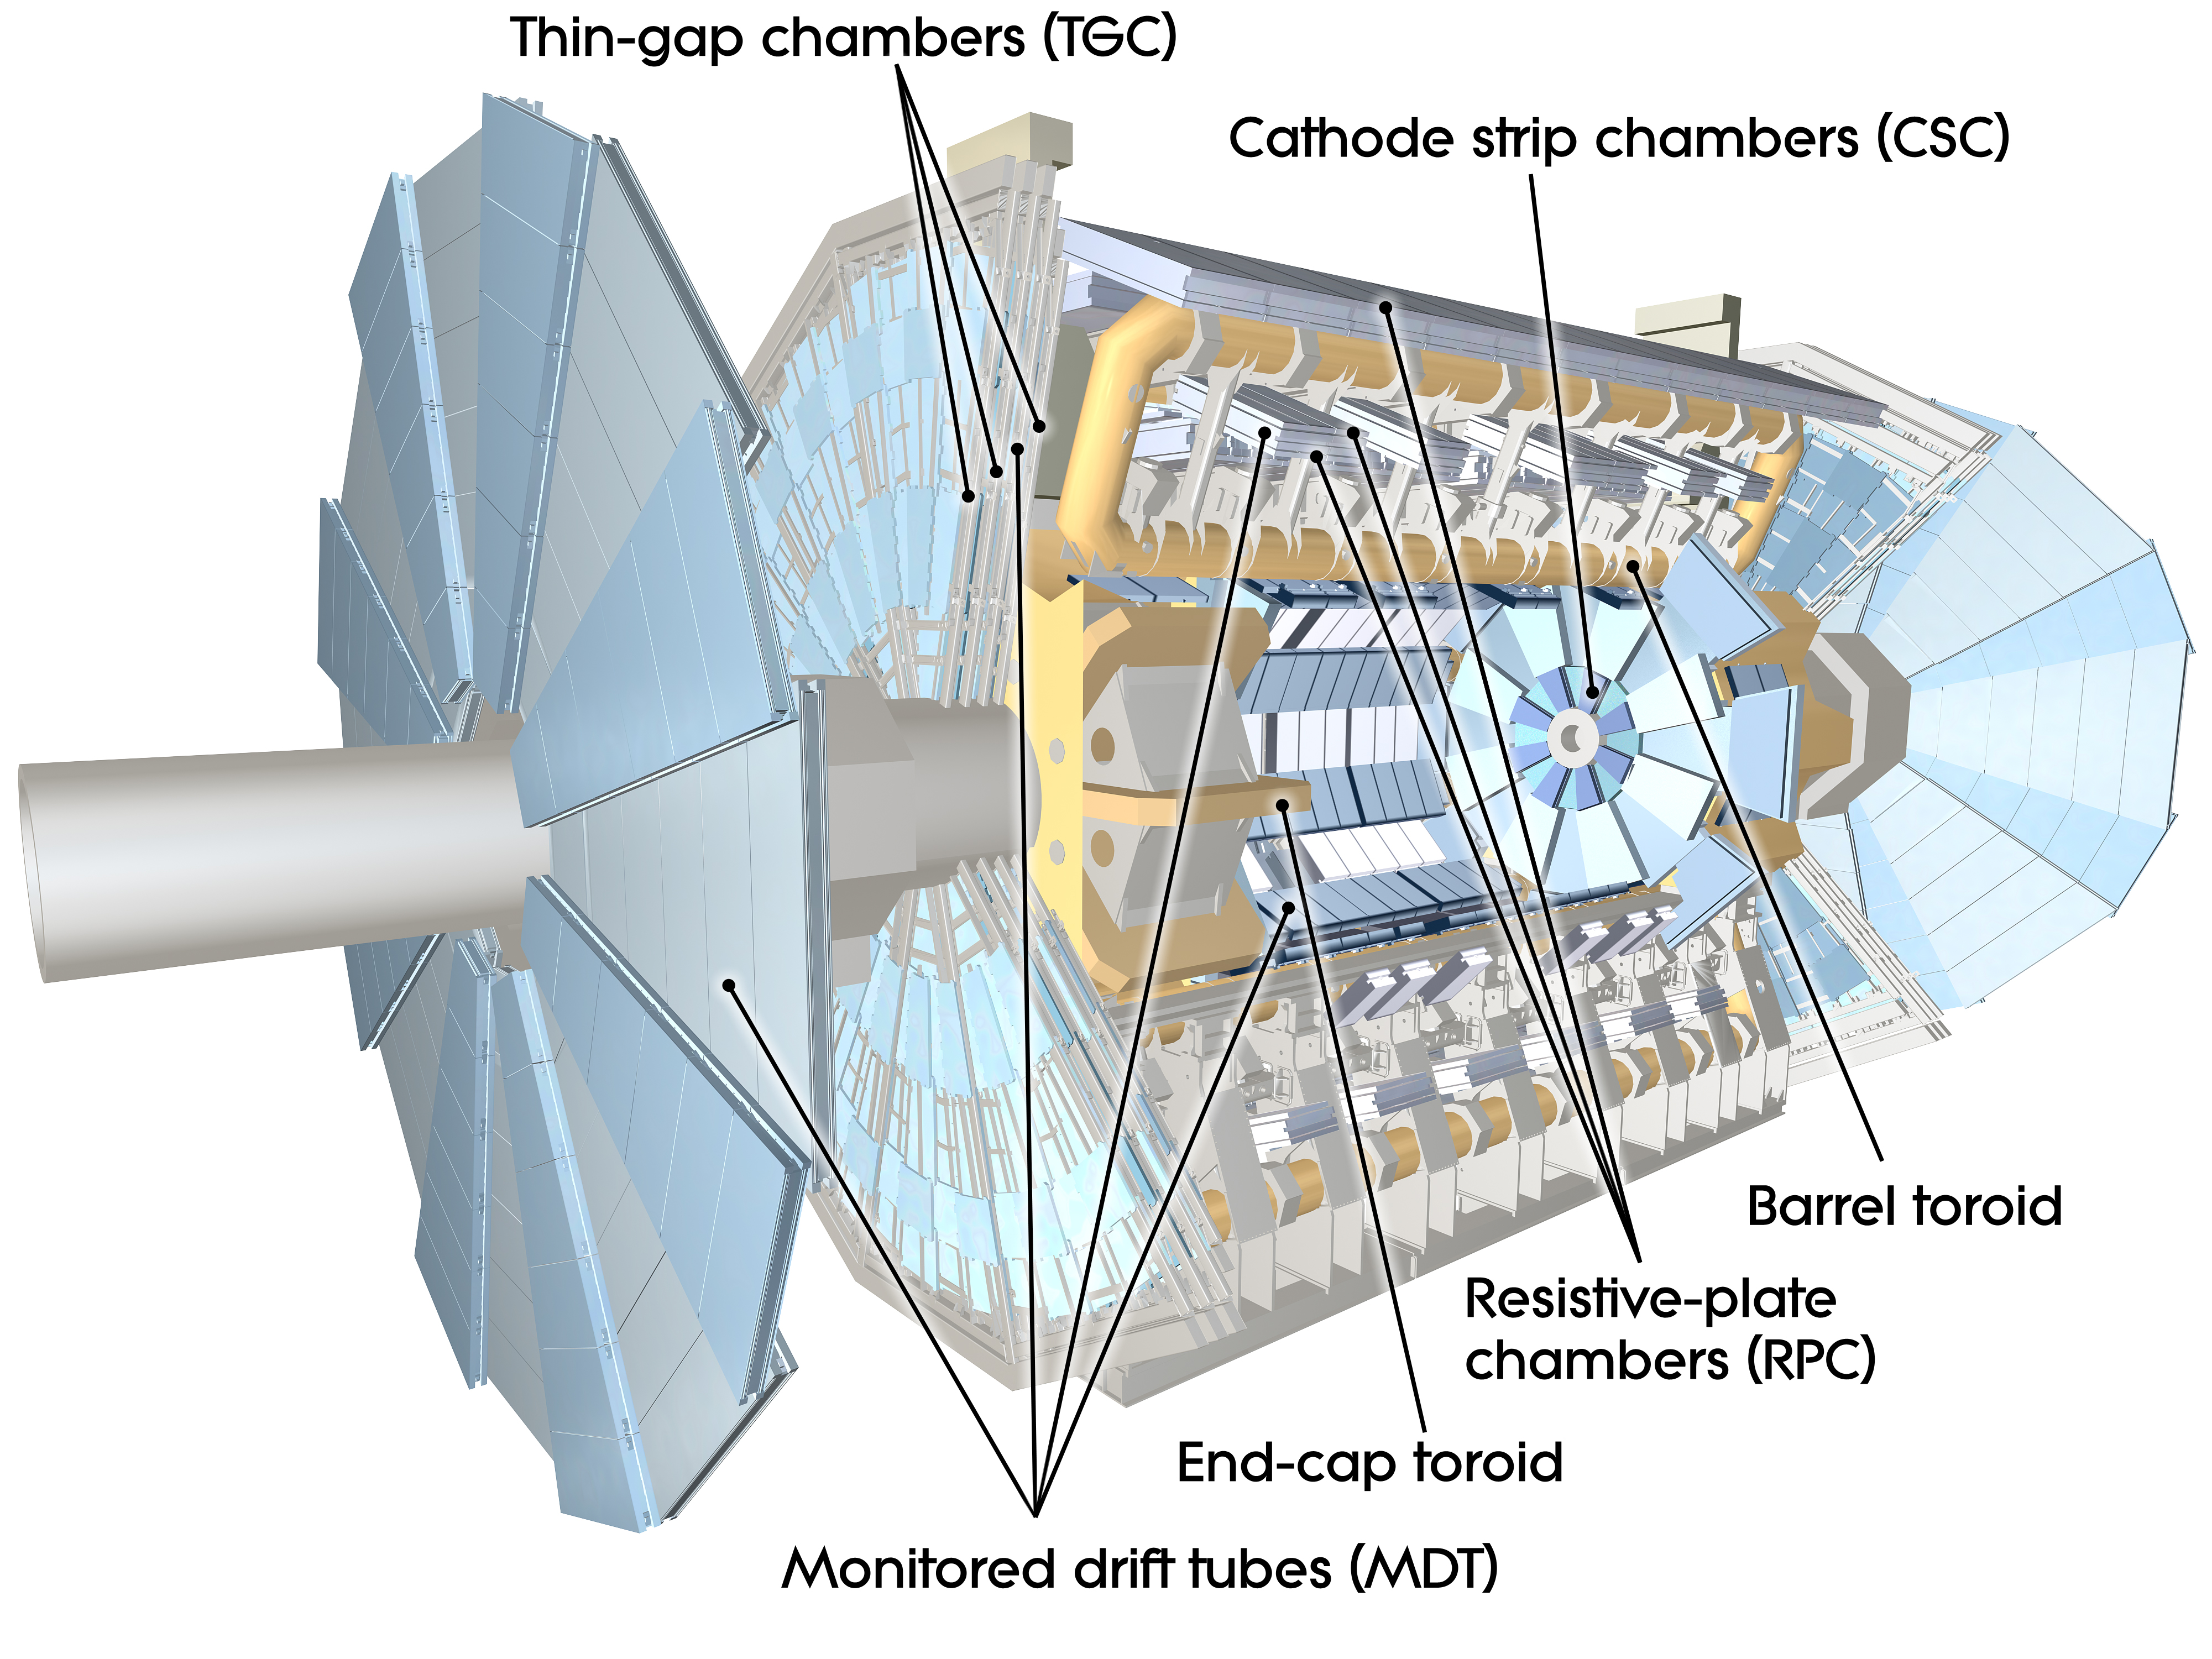
\includegraphics[width=.7\textwidth]{ATLAS-muon-spec}
  \caption[ATLAS muon subsystem]{Computer generated image of the ATLAS Muons
    subsystem~\cite{ATLAS-muon-fig}.}%
  \label{fig:ATLAS-muon}
\end{figure}

\subsection{Trigger Systems}%
\label{sec:trigger}

The trigger systems in ATLAS allows data to be recorded only when an event meets
certain criteria. Without triggering there would be no way to decide which
events to readout and which to ignore. It would be impossible to readout every
interaction that occurs in the detector. The reason for this is that the
geometric constraints of the detector mean that there is only a small space
available for readout wires, as detection medium needs to be prioritized for
sensitivity and technology limits the data rate that one can achieve through a
cable of fixed area. The trigger system comes in two parts, a hardware component
referred to as level one (L1) and software component referred to as the high
level trigger (HLT). The L1 system is comprised of the L1 calorimeter (L1Calo)
trigger which operates by searching for clusters of energy in the calorimeters
and the L1 muon (L1Muon) system which coincidences in the muon systems. A third
system L1 topological (L1Topo) uses regions of interest built from the L1Calo
and L1Muon data which are passed to central trigger processors for selection.
The various limitations of the hardware mean that these selections must be
passed up to the next level of triggering, the HLT in a time window of
2.5~$\mu$s. The HLT takes information from the L1 systems and uses faster
versions of an offline style analysis in order to select or reject events for
readout. In order for a  trigger to fire an event must pass fully all of the
requirements of one of the algorithms defined by an extensive trigger menu. More
information about the triggers used in the $VH(bb)$ analysis will be given in a
later chapter.

\chapter{Machine Learning}%
\label{ch:ml}

The next chapter is somewhat of a diversion from the physics discussed so far.
It will focus on techniques in machine learning which are often referred to in
High Energy Physics as a Multi-variate Analysis (MVA). The reason for this
diversion is that these techniques have become very widespread in the field,
they are used in several of the reconstruction and selection algorithms that are
used to obtain the events on which the analysis is performed. Furthermore an MVA
is used to obtain the distribution that acts as the final discriminant for the
analysis, and machine learning techniques are also used to model the
backgrounds. Given how widespread the use of these techniques is in the analysis
it makes sense to describe them before diving into the details.

The two main algorithms used are Boosted Decision Trees (BDTs) and Neural
Networks (NNs) which will be described in sections~\ref{sec:bdts}
and~\ref{sec:neural-networks} respectively. These algorithms are used in many
places outside High Energy Physics and so rather than referring to individual
pieces of data that enter into the algorithm as an event, in this chapter they
will be referred to as an example. This terminology comes from the fact that in
general these algorithms must be shown a large number of examples before they
are suitable ``trained'' for their purpose, and that in general those examples
could be data that represent anything. Both of these algorithms can be operated
in classification or regression modes. The main difference between these modes
is that classification mode provides a score for each of a given number of
classes which can be interpreted as a probability that a given example belongs
to the given class, whereas regression outputs a single number per example whose
interpretation depends on the problem.

Both algorithms can be written as a function of some inputs $\vec{x}$, some
weights to be found during training $\vec{w}$, and a set of hyper-parameters
$\vec{\theta}$ as follows
\begin{equation}
  F(\vec{x}, \vec{w}, \vec{\theta}) = \vec{y},
  \label{eq:ml-general}
\end{equation}
where $\vec{y}$ is a vector whose outputs correspond to each class in a
classification problem. If the algorithm is set up for a regression problem then
the output will just be one number. The hyper-parameters control the behaviour
of the algorithm in question and are set by hand in advance of training.
Training either algorithm involves an iterative process where at each iteration
the function is evaluated for the current set of weights, the outputs are
compared against some truth labels $\vec{t}$ via the computation of a loss
function. Based on the value of the loss function the weights are then updated
according to the given algorithm. It is therefore vital that firstly these truth
labels are available for the data on which one wants to train (e.g. train on
simulated predictions rather than real data) and secondly that the examples are
split into a training and testing set so that the set which is used to
iteratively update weights is not the same set that performance is evaluated on.
This avoids over-fitting to any noise in a given set, though this problem is not
circumvented entirely and over-fitting will be addressed for specific algorithms
in the sections ahead.

\section{Boosted Decision Trees}%
\label{sec:bdts}
We will start by discussing a decision tree for a classification problem.
Decision trees have a structure as in figure~\ref{fig:bdt}, which shows a tree
dividing examples into two classes, red and blue.
\begin{figure}[h]
  \centering
  \begin{tikzpicture}
    \draw [very thick] plot [smooth] coordinates {(-5,-3) (5,3)};
    \draw [very thick] plot [smooth] coordinates {(-5, 3) (5,-3)};
  \end{tikzpicture}
  \caption{The structure of a decision tree.}
  \label{fig:bdt}
\end{figure}


Each circular node in the tree represents a cut on one of a number of variables
provided as input to the algorithm. The tree is read top to bottom with each
node being followed by two edges branching left and right that represent the
path taken by examples which pass or fail the cut respectively. Square nodes
represent that the termination criteria have been reached and that events in
these nodes have been classified according to the colour of the node. The
variable chosen at each node is optimised in order to maximise a criteria
related to the separation of classes.  For a problem containing two classes a
common separation criteria is the Gini index,
\begin{equation}
  G = p(1-p),
  \label{eq:gini}
\end{equation}
where p is the purity of a chosen class that one wants to maximise.

A decision tree by itself is able to separate examples into a number of classes,
however a single tree is prone to over--training. Over--training is the term
used to describe the phenomena where a classifier learns from statistical
fluctuations in the data rather learning a generalised separation boundary
between classes. The reason that decision trees are susceptible to this is that
if two variables yield a similar separation criteria then a fluctuation in the
training data may lead to the choice of one variable over another for a
particular node, this choice will lead to a very different tree structure than
if the fluctuation were not present.

In order to mitigate the over--training tendencies of decision trees they are
often used in an ensemble algorithm such as bagging~\cite{bagging}
or boosting~\cite{boosting}. Here only boosting will be discussed. Ensembles of
decision trees are often referred to as random forests. Boosting works by
training a sequence of trees, weighting misclassified events from a tree so that
they have more influence over the structure of the next tree in the sequence.
The final classification of any given example is a weighted average over all
trees, this can be weighted by the overall accuracy of each tree, but in general
can take any weighted average.

\subsection{Gradient Boosting}

Gradient boosting is the name of an optimisation algorithm that takes the
concept of boosting and combines it with the gradient descent algorithm. A
pictographic representation of gradient descent for a regression problem can be
seen in figure~\ref{fig:grad-desc.}
\begin{figure}[ht]
  \centering
  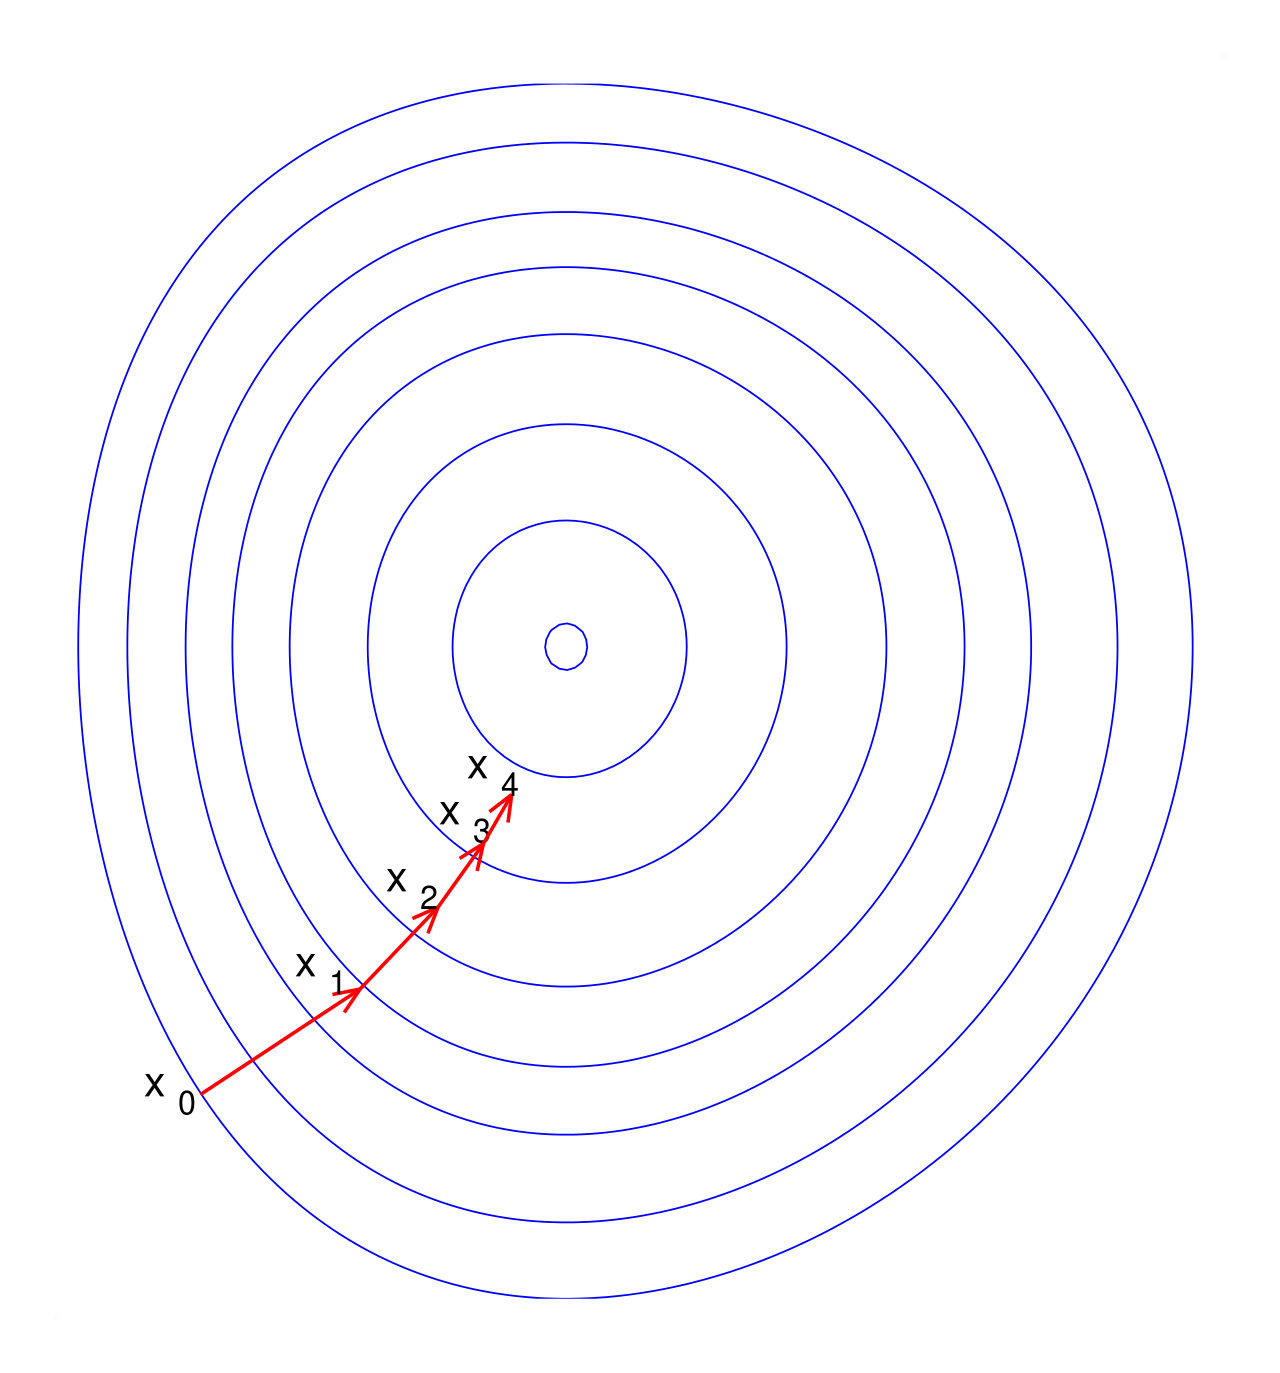
\includegraphics[width=.6\textwidth]{gradient-descent}
  \caption[An illustration of gradient descent.]{An illustration of the gradient
    descent algorithm. The blue lines represent level sets of a function, sets
    of points that have the same gradient. The $x$'s represent where in along
    the function the algorithm is at a given step with the steps numbered 0 to
    4.}
  \label{fig:grad-desc}
\end{figure}
  

\section{Neural Networks}%
\label{sec:neural-networks}
Neural networks have a structure as in figure~\ref{fig:nn}.

This section outlines some of the mathematical formalism surrounding NNs
that act as classifiers. These kinds of NNs can be used to solve binary
classification or multi-class problems, where the probability that each data
candidate belongs to any of the classes is mutually exclusive. Many other types
of NN exist, however their details will not be discussed in this work. In simple
terms a NN is comprised of connected layers of nodes as in figure
\ref{fig:basicnn}. Nodes fall into three types input, output and hidden, with
layers being homogeneous with regard to node type and therefore inheriting their
name. The input layer is comprised of one input node per dimension of a single
entry in the dataset that one wishes to pass into the NN for classification.
Each output node is a predictive unit corresponding to one of $K$ classes and it
is the goal of the intermediate hidden layers (full of hidden units) to provide
a relationship between the inputs and outputs such that the predictive unit with
the highest value corresponds to the correct class for the given data. The
output layer should therefore be comprised of $K$ nodes. In order to delve
further into the details, a good mathematical representation of the hidden
layers is required. One such representation is given by Bishop in Pattern
Recognition and Machine Learning \cite{PRML}. In this section the nomenclature
used by Bishop will be outlined and then adapted for our specific use.

\tikzset{%
  every neuron/.style={
    circle,
    minimum size=22pt,
    draw
  },
  neuron missing/.style={
    draw=none, 
    scale=3,
    text height=0.3cm,
    execute at end node=\color{black}\tiny{$\vdots$}
  },
}

\begin{figure}[hbtp]
  \centering
  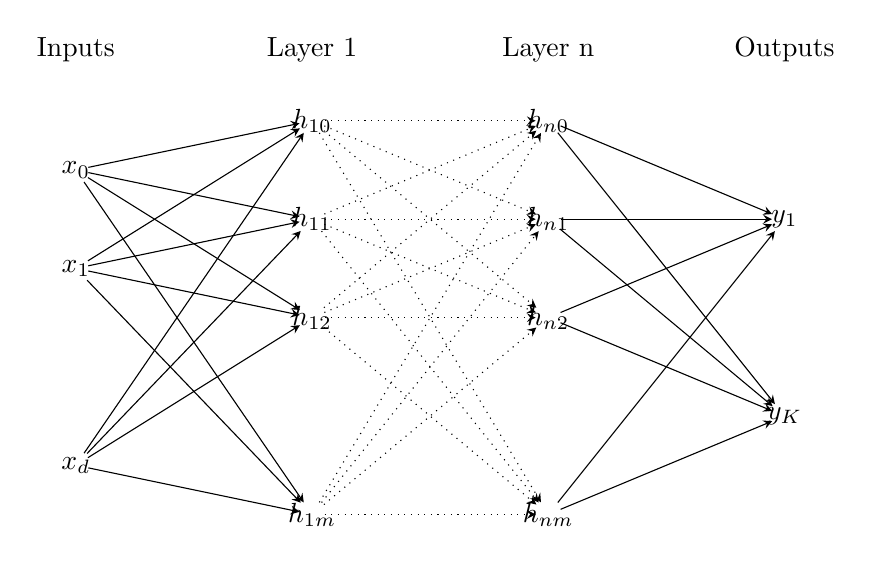
\begin{tikzpicture}[x=1.5cm, y=1.25cm, >=stealth]
    
    \foreach \m/\l [count=\y] in {1,2,missing,3}
    \node [every neuron/.try, neuron \m/.try] (input-\m) at (0,2-\y) {};

    \foreach \m [count=\y] in {1,2,3,missing,4}
    \node [every neuron/.try, neuron \m/.try ] (hidden1-\m) at (2,2.5-\y) {};

    \foreach \m [count=\y] in {1,2,3,missing,4}
    \node [every neuron/.try, neuron \m/.try ] (hidden2-\m) at (4,2.5-\y) {};

    \foreach \m [count=\y] in {1,missing,2}
    \node [every neuron/.try, neuron \m/.try ] (output-\m) at (6,1.5-\y) {};

    \foreach \l [count=\i] in {0,1,d}
    \node at (input-\i.center) {$x_{\l}$};

    \foreach \l [count=\i] in {0,1,2,m}
    \node at (hidden1-\i.center) {$h_{1\l}$};

    \foreach \l [count=\i] in {0,1,2,m}
    \node at (hidden2-\i.center) {$h_{n\l}$};

    \foreach \l [count=\i] in {1,K}
    \node at (output-\i.center) {$y_\l$};

    \foreach \i in {1,...,3}
    \foreach \j in {1,...,4}
    \draw [->, shorten <=1pt, shorten >=1pt] (input-\i) -- (hidden1-\j);

    \foreach \i in {1,...,4}
    \foreach \j in {1,...,4}
    \draw [dotted, ->, shorten <=1pt, shorten >=1pt] (hidden1-\i) -- (hidden2-\j);

    \foreach \i in {1,...,4}
    \foreach \j in {1,...,2}
    \draw [->, shorten <=1pt, shorten >=1pt] (hidden2-\i) -- (output-\j);

    \foreach \l [count=\x from 0] in {Inputs, Layer 1, Layer n, Outputs}
    \node [align=center, above] at (\x*2,2) {\l};
  \end{tikzpicture}
  \caption[A depiction of a neural network.]{A more complex neural network
    containing an input layer of $d$ nodes corresponding to data of dimensionality
    $d$, $n$ hidden layers of $m$ hidden units each $h_{ij}$ (where $i$ indexes
    hidden layer and $j$ indexes a particular unit) and an output layer of $K$
    predictive units $y_k$.}
  \label{fig:nn}
\end{figure}
The building blocks of the NN, called activations, resemble Fisher
discriminants \cite{Fisher} and take the form

\begin{equation}
a_j = \sum_{i=1}^{d} w_{ji}x_{i} + w_{j0}
\label{eq:fisher}
\end{equation}
where the $w_{ji}$ terms are known as weights and the $w_{j0}$ as biases.
Collectively the weights and biases shall be referred to as adaptive parameters,
due to the fact that (as shall be made clear later) they are to be adapted by a
training algorithm. In order to take the activations and turn them into
something closer to a perceptron \cite{Rosenblatt} they must be passed through
an activation function denoted $\mathcal{H}$,

\begin{equation}
h_j = \mathcal{H}(a_j)
\label{eq:hiddenunit}
\end{equation}
becoming what are known as hidden units. These activation functions may be
non-linear and have the restriction that they must be differentiable, crucially
this is different from the perceptron which uses a non-differentiable step
function. Considering a network with only a single hidden layer as in figure
\ref{fig:basicnn}, there are further steps required to get from the hidden units
to the predictions $y_k$. The complete network function as an argument of a
vector of data points $\vec{x}$ and a matrix of adaptive parameters
$\vec{w}$ should return predictions given by

\begin{equation}
y_k(\vec{x},\vec{w}) = \mathcal{O} \Bigg( \sum_{j=1}^{m} w_{kj}^{(2)}
\mathcal{H} \Bigg( \sum_{i=1}^{d} w_{ji}^{(1)} x_{i} + w_{j0}^{(1)} \Bigg) + w_{k0}^{(2)} \Bigg).
\label{eq:basicnn}
\end{equation}
where now, as in Bishop's representation, the superscript number in brackets
labels the layer to which adaptive parameters belong, not counting the input
layer (as it does not contain them). The network function \eqref{eq:basicnn} is
comprised by performing the same construction on the hidden unit
\eqref{eq:hiddenunit} as was performed on the original data point $x_i$ in
\eqref{eq:fisher}, with a special type of activation function an output function
$\mathcal{O}$. Notably the hidden units must be summed over in the same way that
data points are, however instead of summing over the dimensions of the data, in
order to reproduce the network in figure \ref{fig:basicnn} we sum up to $m$ the
desired number of hidden units, which is referred to as the ``size'' of the
hidden layer. A common choice of output function for binary classification
problems is the logistic sigmoid function
\begin{equation}
\mathcal{O}(z) = \frac{1}{1 + exp(-z)}
\label{eq:sigmoid}
\end{equation}
where in each of these $z$ merely denotes the argument of the output function.
For multi-class problems where $K > 2$ a generalisation of the logistic sigmoid,
the softmax function
\begin{equation}
\mathcal{O}(z)_k = p(k|\vec{x}) = \frac{exp(z_k)}{\sum_{i=1}^kexp(z_i)}
\label{eq:softmax}
\end{equation}
gives the probability of being in class $k$ given the data $\vec{x}$ and
where $i$ is summed all classes. The index $k$ appears on the output function as
it must be calculated for each $k \in K$ the total number of classes. It is at
this stage that the true meaning of the predictive units is solidified, each
should give a number between zero and one that represents the probability of
data belonging to the corresponding class, and logically all predictive units
should sum to one. For the sake of compactness we shall, as Bishop does,
re-write \eqref{eq:basicnn} by introducing $x_{0} = 1$ in order to absorb the
biases into the sums, yielding
\begin{equation}
y_k(\vec{x},\vec{w}) = \mathcal{O} \Bigg( \sum_{j=0}^{m} w_{kj}^{(2)}
\mathcal{H} \Bigg( \sum_{i=0}^{d} w_{ji}^{(1)} x_{i} \Bigg) \Bigg).
\label{eq:compactnn}
\end{equation}
\par Now it is our goal to generalise this network function to one not only of
an arbitrary number of hidden layers but also such that each hidden layer can be
of arbitrary size and have an arbitrary activation function. For this purpose,
networks will now be described in terms of the number of hidden layers, instead
of the number of layers that contain adaptive parameters (hidden plus output) as
before. We may start by writing a function for a network of two hidden layers
\begin{equation}
y_k(\vec{x},\vec{w}) = \mathcal{O} \Bigg( \sum_{j_{2}=0}^{m_{2}} w_{kj_{2}} \mathcal{H}_{2} 
\Bigg( \sum_{j_{1}=0}^{m_{1}} w_{j_{2}j_{1}} \mathcal{H}_{1} \Bigg( \sum_{i=0}^{d} w_{j_{1}i} x_{i} \Bigg) \Bigg) \Bigg).
\label{eq:2layer}
\end{equation}
In order to arive at the two layer function \eqref{eq:2layer} the same process
was used as for the original network function \eqref{eq:basicnn}. Now there are
two activation functions and hidden layer sizes denoted $m$. Clearly adding a
layer to the network simply involves repeated application of this process and
picking up the required number of additional parameters. A function for a
network of $n$ hidden layers may therefore be written as
\begin{equation}
y_k(\vec{x},\vec{w}) = \mathcal{O} \Bigg( \sum_{j_{n}=0}^{m_{n}} w_{kj_{n}}
\mathcal{H}_{n} \Bigg( \dots \mathcal{H}_2  \Bigg( \sum_{j_{1}=0}^{m_{1}} w_{j_{2}j_{1}} 
\mathcal{H}_{1} \Bigg( \sum_{i=0}^{d} w_{j_{1}i} x_{i} \Bigg) \Bigg) \dots \Bigg) \Bigg)
\label{eq:fullnn}
\end{equation}
where there are $n$ different versions of the activation function and hidden
layer size. Our new hidden units obey the following notation
\begin{equation}
h_{nj} = \mathcal{H}_n(a_j)
\label{eq:newhiddenunits}
\end{equation}
eliminating the need for the superscript labelling of layer. The new labelling
identifies hidden layer by the left-hand index of the hidden unit or the
right-hand hidden layer of the weights and biases. In equation \eqref{eq:fullnn}
the hidden units are shown in their expanded form and distinguished by the fact
that their $j$ indices take on the subscript of $n$ corresponding to the layer
they belong to. Figure \ref{fig:fullnn} depicts a network of $n$ hidden layers,
as described in equation \eqref{eq:fullnn} except that every hidden layer is
depicted with the same size $m$.

\tikzset{%
  every neuron/.style={
    circle,
    minimum size=22pt,
    draw
  },
  neuron missing/.style={
    draw=none, 
    scale=3,
    text height=0.3cm,
    execute at end node=\color{black}\tiny{$\vdots$}
  },
}

\begin{figure}[hbtp]
  \centering
  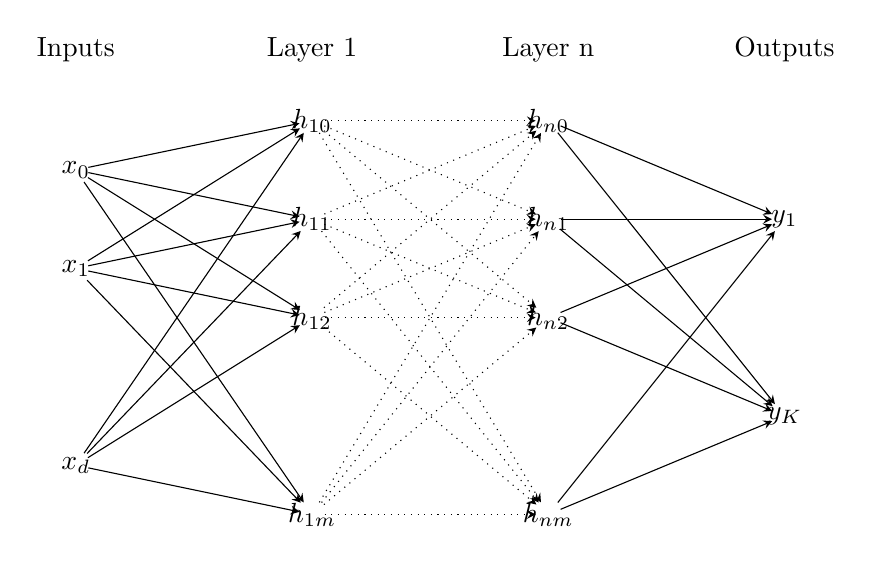
\begin{tikzpicture}[x=1.5cm, y=1.25cm, >=stealth]
    
    \foreach \m/\l [count=\y] in {1,2,missing,3}
    \node [every neuron/.try, neuron \m/.try] (input-\m) at (0,2-\y) {};

    \foreach \m [count=\y] in {1,2,3,missing,4}
    \node [every neuron/.try, neuron \m/.try ] (hidden1-\m) at (2,2.5-\y) {};

    \foreach \m [count=\y] in {1,2,3,missing,4}
    \node [every neuron/.try, neuron \m/.try ] (hidden2-\m) at (4,2.5-\y) {};

    \foreach \m [count=\y] in {1,missing,2}
    \node [every neuron/.try, neuron \m/.try ] (output-\m) at (6,1.5-\y) {};

    \foreach \l [count=\i] in {0,1,d}
    \node at (input-\i.center) {$x_{\l}$};

    \foreach \l [count=\i] in {0,1,2,m}
    \node at (hidden1-\i.center) {$h_{1\l}$};

    \foreach \l [count=\i] in {0,1,2,m}
    \node at (hidden2-\i.center) {$h_{n\l}$};

    \foreach \l [count=\i] in {1,K}
    \node at (output-\i.center) {$y_\l$};

    \foreach \i in {1,...,3}
    \foreach \j in {1,...,4}
    \draw [->, shorten <=1pt, shorten >=1pt] (input-\i) -- (hidden1-\j);

    \foreach \i in {1,...,4}
    \foreach \j in {1,...,4}
    \draw [dotted, ->, shorten <=1pt, shorten >=1pt] (hidden1-\i) -- (hidden2-\j);

    \foreach \i in {1,...,4}
    \foreach \j in {1,...,2}
    \draw [->, shorten <=1pt, shorten >=1pt] (hidden2-\i) -- (output-\j);

    \foreach \l [count=\x from 0] in {Inputs, Layer 1, Layer n, Outputs}
    \node [align=center, above] at (\x*2,2) {\l};
  \end{tikzpicture}
  \caption[A depiction of a neural network.]{A more complex neural network
    containing an input layer of $d$ nodes corresponding to data of dimensionality
    $d$, $n$ hidden layers of $m$ hidden units each $h_{ij}$ (where $i$ indexes
    hidden layer and $j$ indexes a particular unit) and an output layer of $K$
    predictive units $y_k$.}
  \label{fig:nn}
\end{figure}
There are now a great deal of parameters that we have to keep track of. It
is therefore important to distinguish between adaptive parameters and the
parameters which we must pick by hand, known as hyper-parameters. A relationship
can be written between the number of hidden layers $n$, and the number of
hyper-parameters, as follows
\begin{equation}
\text{\# of hyper-parameters} = 2n + 1.
\label{eq:hyper}
\end{equation}
As previously stated there are simply $n$ lots of activation functions and $n$
hidden layers to determine a size for. Often it is sufficient to set all
activation functions to the same function, and in this work all hidden layers
share the same size for simplicity. The adaptive parameters are far more
numerous, and will be optimised by means of a training algorithm. In TensorFlow
the variable object is choice for implementing the adaptive parameters as
training algorithms in the software will update them by default. The adaptive
parameters are initialised randomly from a Gaussian distribution resulting in
poor predictive power to begin with. In order to improve this some figure of
merit, known as a loss function, must be used in order for the training
algorithm to measure quantitatively the performance of the NN. We also must
provide the algorithm with a dataset to train on, complete with a set of targets
or labels that, for the training set, reveal the correct classification for each
entry. Due to the this requirement, methods such as these are referred to as
supervised learning methods. A natural loss function one may use to describe the
error of the model given a current set of adaptive parameters is sum-of-squares
error
\begin{equation}
E(\vec{w}) = \frac{1}{2}\sum_{n=1}^{N}(y(\vec{x}_n, \vec{w}) - t_n)^2
\label{eq:sumofsquares}
\end{equation}
where $t_n$ are the targets for the given data entries $\vec{x}_n$.
Minimising this function with some algorithm does work in practice, however it
has been shown that, using
\begin{equation}
E(\vec{w}) = - \sum_{n=1}^{N} \Bigg (t_n \ln (y_n) + (1-t_n) \ln (1-y_n) \Bigg)
\label{eq:xentropy}
\end{equation}
known as cross-entropy, is faster and more generalised \cite{XEntropySimard}
(further discussion on generalisation in section \ref{sec:generalisation}). The
particular training algorithm that will be used to update parameters in this
report is known as adaptive moment estimation or ADAM \cite{ADAMOpt}. ADAM is a
variant of the gradient descent algorithm, which is widely used and has spawned
many other variants \cite{GDOverview}. The reasons for picking between ADAM and
vanilla gradient descent are given in chapter \ref{ch:netarch}.

\tikzset{%
  every neuron/.style={
    circle,
    minimum size=22pt,
    draw
  },
  neuron missing/.style={
    draw=none, 
    scale=3,
    text height=0.3cm,
    execute at end node=\color{black}\tiny{$\vdots$}
  },
}

\begin{figure}[hbtp]
  \centering
  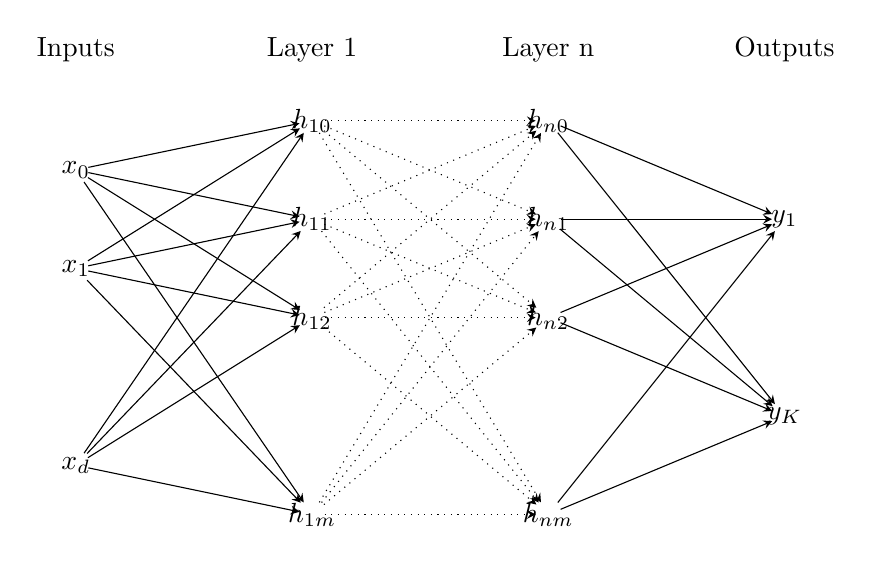
\begin{tikzpicture}[x=1.5cm, y=1.25cm, >=stealth]
    
    \foreach \m/\l [count=\y] in {1,2,missing,3}
    \node [every neuron/.try, neuron \m/.try] (input-\m) at (0,2-\y) {};

    \foreach \m [count=\y] in {1,2,3,missing,4}
    \node [every neuron/.try, neuron \m/.try ] (hidden1-\m) at (2,2.5-\y) {};

    \foreach \m [count=\y] in {1,2,3,missing,4}
    \node [every neuron/.try, neuron \m/.try ] (hidden2-\m) at (4,2.5-\y) {};

    \foreach \m [count=\y] in {1,missing,2}
    \node [every neuron/.try, neuron \m/.try ] (output-\m) at (6,1.5-\y) {};

    \foreach \l [count=\i] in {0,1,d}
    \node at (input-\i.center) {$x_{\l}$};

    \foreach \l [count=\i] in {0,1,2,m}
    \node at (hidden1-\i.center) {$h_{1\l}$};

    \foreach \l [count=\i] in {0,1,2,m}
    \node at (hidden2-\i.center) {$h_{n\l}$};

    \foreach \l [count=\i] in {1,K}
    \node at (output-\i.center) {$y_\l$};

    \foreach \i in {1,...,3}
    \foreach \j in {1,...,4}
    \draw [->, shorten <=1pt, shorten >=1pt] (input-\i) -- (hidden1-\j);

    \foreach \i in {1,...,4}
    \foreach \j in {1,...,4}
    \draw [dotted, ->, shorten <=1pt, shorten >=1pt] (hidden1-\i) -- (hidden2-\j);

    \foreach \i in {1,...,4}
    \foreach \j in {1,...,2}
    \draw [->, shorten <=1pt, shorten >=1pt] (hidden2-\i) -- (output-\j);

    \foreach \l [count=\x from 0] in {Inputs, Layer 1, Layer n, Outputs}
    \node [align=center, above] at (\x*2,2) {\l};
  \end{tikzpicture}
  \caption[A depiction of a neural network.]{A more complex neural network
    containing an input layer of $d$ nodes corresponding to data of dimensionality
    $d$, $n$ hidden layers of $m$ hidden units each $h_{ij}$ (where $i$ indexes
    hidden layer and $j$ indexes a particular unit) and an output layer of $K$
    predictive units $y_k$.}
  \label{fig:nn}
\end{figure}
\section{Parametrised Neural Networks}%
\label{sec:param-neural-nets}
Parametrised neural networks take extra inputs equal to the number of relevant
parameters, as seen in figure~\ref{fig:pnn}.
% UNUSED
% \begin{figure}[hbtp]
% \begin{center}
% \begin{tikzpicture}[x=1.5cm, y=1.25cm, >=stealth]

% \foreach \m/\l [count=\y] in {1,2,missing,3}
%   \node [every neuron/.try, neuron \m/.try] (input-\m) at (0,2-\y) {};

% \foreach \m [count=\y] in {1,2,3,missing,4}
%   \node [every neuron/.try, neuron \m/.try ] (hidden1-\m) at (2,2.5-\y) {};

% \foreach \m [count=\y] in {1,2,3,missing,4}
%   \node [every neuron/.try, neuron \m/.try ] (hidden2-\m) at (4,2.5-\y) {};

% \foreach \m [count=\y] in {1,missing,2}
%   \node [every neuron/.try, neuron \m/.try ] (output-\m) at (6,1.5-\y) {};

% \foreach \l [count=\i] in {0,1,d}
%   \node at (input-\i.center) {$x_{\l}$};

% \foreach \l [count=\i] in {0,1,2,m}
%   \node at (hidden1-\i.center) {$h_{1\l}$};

%   \foreach \l [count=\i] in {0,1,2,m}
%   \node at (hidden2-\i.center) {$h_{n\l}$};

% \foreach \l [count=\i] in {1,K}
%   \node at (output-\i.center) {$y_\l$};

% \foreach \i in {1,...,3}
%   \foreach \j in {1,...,4}
%     \draw [->, shorten <=1pt, shorten >=1pt] (input-\i) -- (hidden1-\j);

% \foreach \i in {1,...,4}
%   \foreach \j in {1,...,4}
%     \draw [dotted, ->, shorten <=1pt, shorten >=1pt] (hidden1-\i) -- (hidden2-\j);

% \foreach \i in {1,...,4}
%   \foreach \j in {1,...,2}
%     \draw [->, shorten <=1pt, shorten >=1pt] (hidden2-\i) -- (output-\j);

% \foreach \l [count=\x from 0] in {Inputs, Layer 1, Layer n, Outputs}
%   \node [align=center, above] at (\x*2,2) {\l};

% \end{tikzpicture}
% \caption{A more complex neural network containing an input layer of $d$ nodes corresponding to data of dimensionality $d$, $n$ hidden layers of $m$ hidden units each $h_{ij}$ (where $i$ indexes hidden layer and $j$ indexes a particular unit) and an output layer of $K$ predictive units $y_k$.}
% \label{fig:pnn}
% \end{center}
% \end{figure}



\chapter{Reconstruction and Selection}%
\label{sec:method}
\section{Channel Definitions and Selections}%
\label{sec:channels-and-selections}
\subsection{Top \texorpdfstring{$e \mu$}{e mu} control region}%
\label{sec:topemucr}
\subsection{\texorpdfstring{$\Delta R(b,b)$}{DRbb} Control Regions}%
\label{sec:control-region-defintions}



\chapter{Analysis Strategy}%
\label{ch:strategy}
In the previous chapter the process of reconstruction and selection was
described. With the objects required for this analysis reconstructed and an
event selection in place an analysis strategy is formed in order to maximise the
signal strength of the VH(bb) process and yield a robust result that is well
understood in terms of modelling and systematic errors. In this chapter that
strategy will be detailed, first the categorisation into analysis regions will
be defined, next the multi-variate algorithm that is used to generate some of
the distributions entering into the profile-likelihood fit will be explained.
Plots of the data versus Monte-Carlo prediction will then be shown in order to
build a picture of the pre-fit status of the agreement. Finally a series of
cross-checks which are used to validate the methods of the analysis will be
explained.

The author's contributions include studying the behaviour of the
profile-likelihood fit with the inclusion of these regions, which are new in
this round of the analysis and making comparisons between the 80~\invfb and
140~\invfb datasets). Contributions also include the training of the
multi-variate classification algorithm with the inclusion of new input variables
with respect to the previous version of the algorithm.

\section{Categorisation into Analysis Regions}
\label{sec:ana-regions}

Events which pass the selection detailed in table~\ref{tab:event-selection} are
categorised into several regions for analysis. Firstly they are split into what
are known as medium ($75 - 150 \GeV$), high ($150 - 250 \GeV$) and extreme ($ >
250 \GeV$) $p_T^{V}$. Events are further categorised by jet multiplicity, all
jets are required by the selection to have at least two jets, categories are
defined for events with exactly two, or exactly three jets. In the 2--lepton
channel there is a requirement of three or more jets but when referring to all
three channels at once categorisation is referred to as simply 3-jet or 2-jet.

Furthermore events are categorised into a so-called signal region which is
straddled either side by two control regions. This categorisation is achieved
via continuous cuts defined in the $\Delta R(b, \bar{b})$~---~$p_T^{V}$ plane,
they are chosen to maximise the signal purity in the signal region and are shown
for the 1--lepton channel in figure~\ref{fig:drbb-crs}.
\begin{figure}[h]
  \centering
  \begin{tabular}{cc}
    \subfloat[]{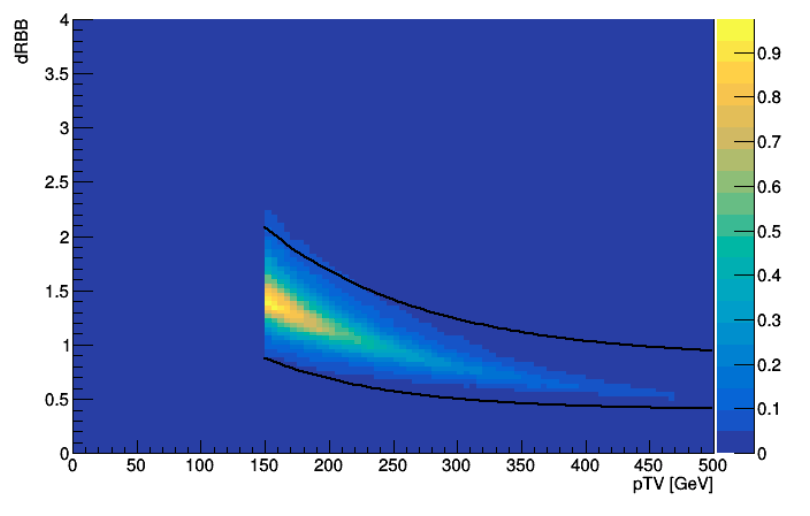
\includegraphics[width=0.505\linewidth]{1lep_qqWH_2tag_2jet.png}}
    \subfloat[]{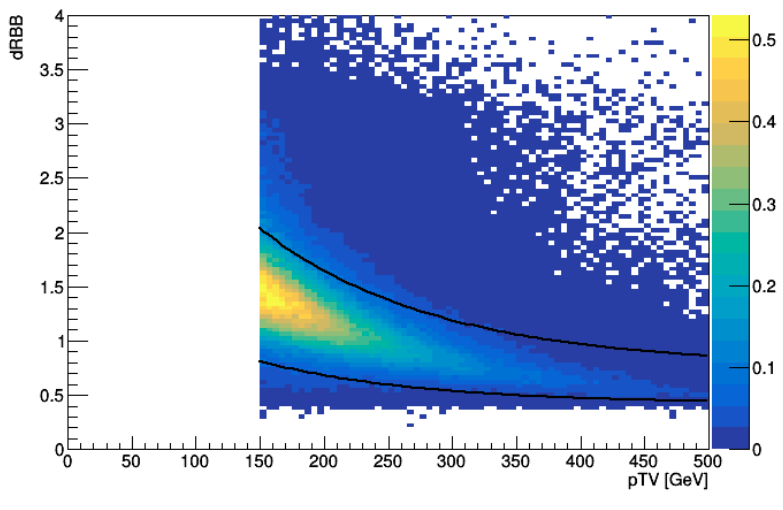
\includegraphics[width=0.49\linewidth]{1lep_qqWH_2tag_3jet.png}}\\
  \end{tabular}
  \caption{Signal distribution of $\Delta R$ between the two selected jets as
    function of $p_{T}^{V}$ in the 1-lepton channel are shown in the 2-tag 2-jet
    (a) and 2-tag 3-jet (b) categories. The black lines demonstrate the upper
    and lower continuous cuts used to categorise the events into the signal and
    control regions}
  \label{fig:drbb-crs}
\end{figure}
The control regions either side of the signal region are known as the
high-$\Delta R(b, \bar{b})$ and low-$\Delta R(b, \bar{b})$ regions, shortened to
CRHigh and CRLow respectively.

A 3D representation of the regions defined when combining these three
categorisations can be seen in figure~\ref{fig:analysis-categories}.
\begin{figure}[ht]
  \centering
  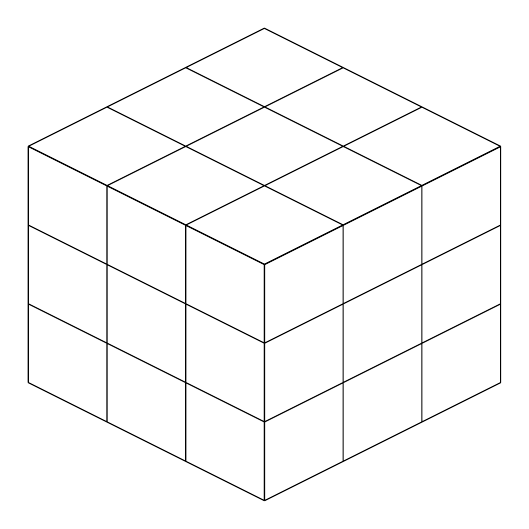
\begin{tikzpicture}[every node/.style={minimum size=1cm},on grid]
\begin{scope}[every node/.append style={yslant=-0.5},yslant=-0.5]
  \path (0,0) rectangle +(3,3);
  \node at (0.5,2.5) {};
  \node at (1.5,2.5) {};
  \node at (2.5,2.5) {};
  \node at (0.5,1.5) {};
  \node at (1.5,1.5) {};
  \node at (2.5,1.5) {};
  \node at (0.5,0.5) {};
  \node at (1.5,0.5) {};
  \node at (2.5,0.5) {};
  \draw (0,0) grid (3,3);
\end{scope}
\begin{scope}[every node/.append style={yslant=0.5},yslant=0.5]
  \path (3,-3) rectangle +(3,3);
  \node at (3.5,-0.5) {};
  \node at (4.5,-0.5) {};
  \node at (5.5,-0.5) {};
  \node at (3.5,-1.5) {};
  \node at (4.5,-1.5) {};
  \node at (5.5,-1.5) {};
  \node at (3.5,-2.5) {};
  \node at (4.5,-2.5) {};
  \node at (5.5,-2.5) {};
  \draw (3,-3) grid (6,0);
\end{scope}
\begin{scope}[every node/.append style={
    yslant=0.5,xslant=-1},yslant=0.5,xslant=-1
  ]
  \path (6,3) rectangle +(-3,-3);
  \node at (3.5,2.5) {};
  \node at (3.5,1.5) {};
  \node at (3.5,0.5) {};
  \node at (4.5,2.5) {};
  \node at (4.5,1.5) {};
  \node at (4.5,0.5) {};
  \node at (5.5,2.5) {};
  \node at (5.5,1.5) {};
  \node at (5.5,0.5) {};
  \draw (3,0) grid (6,3);
\end{scope}
\end{tikzpicture}
\caption{A graphic representation of the analysis categories.}
\label{fig:analysis-categories}
\end{figure}

Note that not all regions of the cube are populated with events in every channel, the medium
$p_T^V$ region is only filled for the 2--lepton channel.

\subsection{Top \texorpdfstring{$e \mu$}{e mu} control region}%
\label{sec:topemucr}

One more region exists only in the 2--lepton channel, it is obtained by inverting the
requirement of two same flavour leptons, requiring two opposite flavour leptons
instead, and keeping all other selection criteria the same. This region contains
almost all $t\bar{t}$ and single top processes (whose Feynman diagrams belong to
the same sum) matching very closely the number of expected events of each of
these backgrounds in the 2--lepton channel. This region is therefore called the
top $e \mu$ control region. The data from this control region can be used as a
prediction for the number of top process events in the 2--lepton channel once
multiplied by a scale factor which accounts for differences in normalisation.
Since data are used as the prediction for these events modelling of shape or
migration between control regions becomes unnecessary.

Plots of top e-mu control region

\section{Composition of Analysis Regions}

This section will detail the composition of each analysis region in terms of
background and signal processes. For all regions the signal process is
$VH~\rightarrow~b\bar{b}$, the prediction for which comes from events generated
using \textsc{Powheg MiNLO}~+~\textsc{Pythia~8} for quark initiated processes
and \textsc{Powheg}~+~\textsc{Pythia~8} for gluon initiated processes as can be
seen in table~\ref{tab:sigMC}.
 
\begin{table}[tbph]
\centering
\resizebox{\textwidth}{!}{
  \begin{tabular}{llrS[table-format=3.2]S[table-format=3.2]S[table-format=3.2]}
    \toprule
    {\bfseries Process} & {\bfseries Generator} & \bfseries{$\bm{\sigma \times BR}$ [pb]} & \multicolumn{3}{c}{{\bfseries $\bm{N_{\text{events}}}$ in millions}}\\
                        &&&\bfseries{mc16a}&\bfseries{mc16d}&\bfseries{mc16e}\\
    \midrule

    $qq \to ZH \to \nu\nu b\bar{b}$ & \textsc{Powheg MiNLO} + \textsc{Pythia 8 } (NNPDF3)& $153.05\times0.582$ & 2  & 2  & 3.3  \\
    $qq \to WH \to l^+\nu b\bar{b}$ & \textsc{Powheg MiNLO} + \textsc{Pythia 8 } (NNPDF3)& $282.78\times0.582$ & 4  & 4  & 6.6  \\
    $qq \to WH \to l^-\nu b\bar{b}$ & \textsc{Powheg MiNLO} + \textsc{Pythia 8 } (NNPDF3) & $179.49\times0.582$ & 2  & 2  & 3.3  \\
    $qq \to ZH \to ll b\bar{b}$ & \textsc{Powheg MiNLO} + \textsc{Pythia 8 } (NNPDF3)& $77.04\times0.582$ & 3  & 3  & 5  \\
    $gg \to ZH \to \nu\nu b\bar{b}$ & \textsc{Powheg} + \textsc{Pythia 8}  (NNPDF3) & $24.57\times0.582$ & 0.5  & 0.5  & 0.5  \\
    $gg \to ZH \to l^{-}l^{+} b\bar{b}$ & \textsc{Powheg} + \textsc{Pythia 8} (NNPDF3) & $12.42\times0.582$ & 0.75  & 0.75  & 0.75  \\
\bottomrule
\end{tabular}
}
\caption{Monte Carlo samples used for the signal processes and the cross section
  and branching ratio (BR) used to normalise the different processes at
  $\sqrt{s}=13$~TeV. Branching ratios correspond to the $H\rightarrow b\bar{b}$
  decay while $V$ branching ratio are still included in the cross-section. This
  was made to make easier the comparison with the reference tables computed
  including $V$ decays in~\cite{twikiCrossSections}. $l$ corresponds to all $e$,
  $\mu$ and $\tau$ leptons together.}
\label{tab:sigMC}
\end{table}


The 0--lepton channel contains the  Z+ jets, W + jets, top quark and diboson
backgrounds. The Z + jets background dominates the mixture in the 2-jet category
across signal and control regions. In the 3-jet category the top-quark processes
dominate apart from in the low $\Delta R(b, \bar{b})$ region. There is very
little signal contamination in the control regions. As can be seen in
table~\ref{tab:bkgMC} V + jets events are generated using \textsc{Sherpa~2.2.1},
top quark events are generated using \textsc{Powheg}~+~\textsc{Pythia~8} and
diboson events are generated also using \textsc{Sherpa~2.2.1}, this is true for
these backgrounds across all channels where a Monte-Carlo prediction is used.

\begin{table}[tbph]
\centering
\resizebox{\textwidth}{!}{
  \begin{tabular}{lllrrrr}
    \toprule
    \multicolumn{2}{l}{{\bfseries Process}} & {\bfseries Generator} & \bfseries{$\bm{\sigma \times BR}$ [pb]} & \bfseries{$\bm{N_{\text{events}}}$ (mc16a)} & \bfseries{$\bm{N_{\text{events}}}$ (mc16d)} & \bfseries{$\bm{N_{\text{events}}}$ (mc16e)}\\
    \midrule
    \multicolumn{2}{l}{\bfseries{Vector boson + jets}} & & & & & \\
    \multicolumn{2}{l}{$Z \to \nu\nu$} & \textsc{Sherpa} $2.2.1$ & $56280\times0.200$ & 150M & 160M & 140M \\
    \multicolumn{2}{l}{$W \to \ell\nu$} & \textsc{Sherpa} $2.2.1$ & $183600\times0.325$ & 340M & 400M & 540M \\
    \multicolumn{2}{l}{$Z/\gamma^{*} \to \ell\ell$} & \textsc{Sherpa} $2.2.1$ & $61940\times0.101$ & 120M & 160M & 210M \\
    \multicolumn{2}{l}{\bfseries{Top-quark}} & & & & & \\
    $t\bar{t}$ & non-full-had (plus MET/pTW extensions) & \textsc{Powheg} + \textsc{Pythia 8} & $831.76\times0.543$ & 120M(55M) & 150M(55M) & 200M(61M) \\
                                            & di-leptonic & \textsc{Powheg} + \textsc{Pythia 8} & $831.76\times0.105$ & $-$ & 45M & 100M \\
    Single-top & $s$~-~channel (leptonic-top) & \textsc{Powheg} + \textsc{Pythia 8} & $10.32\times0.325$ & 4M & 5M & 7M \\
                                            & $t$~-~channel (leptonic-top) & \textsc{Powheg} + \textsc{Pythia 8} & $216.96\times0.325$ & 10M & 12M & 17M \\
                                            & $Wt$~-~channel (plus di-lepton extension)& \textsc{Powheg} + \textsc{Pythia 8} & $71.7\times1$ & 20M & 24M(24M) & 33M(33M) \\
    \multicolumn{2}{l}{\bfseries{Diboson}} & & & & & \\
    $qq\rightarrow WW$ & $\rightarrow qqlv$ & \textsc{Sherpa 2.2.1} & $112.6\times0.439$ & 14M & 50M & 24M \\
    $qq\rightarrow WZ$ & $\rightarrow lvqq$ (with $Z\rightarrow b\bar{b}$ extension) & \textsc{Sherpa 2.2.1} & $50.3\times0.227$ & 7M(6M) & 36M(7M) & 12M(10M) \\
                                            & $\rightarrow qqvv$ & \textsc{Sherpa 2.2.1} & $50.3\times0.135$ & 6M & 6M & 10M \\
                                            & $\rightarrow qqll$ & \textsc{Sherpa 2.2.1} & $50.3\times0.0683$ & 5M & 27M & 9M \\
    $qq\rightarrow ZZ$ & $\rightarrow qqll$ (with $Z\rightarrow b\bar{b}$ extension) & \textsc{Sherpa 2.2.1} & $15.57\times0.140$ & 5M(5M)  & 5M(6M) & 9M(4M) \\
                                            & $\rightarrow qqvv$ (with $Z\rightarrow b\bar{b}$ extension) & \textsc{Sherpa 2.2.1} & $15.57\times0.280$ & 5M(5M)  & 5M(6M) & 9M(8M) \\
    \multicolumn{2}{l}{$gg\rightarrow WW \rightarrow qqlv$} & \textsc{Sherpa 2.2.2} & $4.8\times0.439$ & 0.8M & 0.9M & 1.1M \\
    \multicolumn{2}{l}{$gg\rightarrow ZZ \rightarrow qqll$ or $qqvv$} & \textsc{Sherpa 2.2.2} & $1.57\times0.420$ & 4M & 6M & 8M \\
    \bottomrule
  \end{tabular}
}
\caption{Monte Carlo samples used for the background processes and the cross
  section times branching ratio (BR) used to normalise the different processes
  at $\sqrt{s}=13$ TeV. The last column shows the number of simulated events for
  the {mc16a+d+e} production. Branching ratios correspond to the decays shown.
  In this table $\ell$ is inclusive of $e$, $\mu$, $\tau$ leptons. For
  $Z/\gamma^{*} \to \ell\ell$ events the requirement of $m_{\ell\ell}>40$~GeV
  was imposed.
%For the samples $WZ$ and $ZZ$ the number in brackets shows the number of additional events generated with the decay $Z \rightarrow b\bar{b}$.
}
\label{tbl:bkgMC}
\end{table}


The 1--lepton channel contains the W + jets, Z+ jets, top quark, diboson and multijet
backgrounds where multijet is the name given to backgrounds arising from QCD
processes. The channel is dominated by a mixture of W + jets and top quark
processes, the high $\Delta R(b, \bar{b})$ control region has a higher purity of
top quark processes whereas the low $\Delta R(b, \bar{b})$ control region has a
high purity of W + jets background. Contribution from multijet and Z + jets is
small across all regions, and similarly to in the 0--lepton channel the diboson
background is almost all contained in the signal region.

The 2--lepton channel contains the Z + jets, top quark and diboson backgrounds.
The Z + jets background dominates across all regions particularly in both
$\Delta R(b, \bar{b})$ control regions. Predictions for the top quark processes
are taken from the top $e \mu$ control region described in
section~\ref{sec:topemucr}. Given that these predictions come from data, the
importance of a good understanding of the remaining large background, Z + jets,
is crucial to the performance of the analysis.

\section{Multi-variate Event Classification}%
\label{sec:mva}

The signal regions in all channels enter into the profile-likelihood fit as
distributions generated by a multi-variate analysis. The multi-variate algorithm
used to generate this distribution is a BDT trained to separate
$VH~\rightarrow~b\bar{b}$ from events coming from any other source.
Table~\ref{tab:MVAinputs} shows which variables are used as inputs to algorithm
in each analysis channel and table~\ref{tab:BDTSetup} shows the choice of
hyper-parameters for the algorithm as described in \textsc{tmva}~\cite{TMVA} the
toolkit for multi-variate analysis which is built into
\textsc{ROOT}~\cite{ROOT}, and was used for training this algorithm.
\begin{table}[htbp]
\begin{center}
  \begin{tabular}{lllll}
    \toprule
    {\bfseries Variable} & {\bfseries Name} & {\bfseries 0-lepton} & {\bfseries 1-lepton} & {\bfseries 2-lepton} \\
    \midrule
    $m_{jj}$ & mBB & $\checkmark$ & $\checkmark$ & $\checkmark$ \\
    $\Delta R(jet_{1}, jet_{2})$ & dRBB & $\checkmark$ & $\checkmark$ & $\checkmark$ \\
    $p_{T}^{\text{jet1}}$ & pTB1 & $\checkmark$ & $\checkmark$ & $\checkmark$ \\
    $p_{T}^{\text{jet2}}$ & pTB2 & $\checkmark$ & $\checkmark$ & $\checkmark$ \\
    $p_{T}^{V}$ & pTV & \checkmark & $\checkmark$ & $\checkmark$ \\
    $\Delta \phi(V, H)$ & dPhiVBB & $\checkmark$ & $\checkmark$ & $\checkmark$ \\
    binned MV2c10(jet$_{1}$) & bin\_MV2c10B1 & $\checkmark$ & $\checkmark$ &  \\
    binned MV2c10(jet$_{2}$) & bin\_MV2c10B2 & $\checkmark$ & $\checkmark$ & \\
    $|\Delta \eta(jet_{1}, jet_{2})|$ & dEtaBB & $\checkmark$ &  &  \\
    $M_{\text{eff}}$ & MEff & $\checkmark$ & & \\
    track based soft MET term & softMET & $\checkmark$ & & \\
    MET & MET & $\equiv p_{T}^{V}$ & $\checkmark$ &  \\
    $\min(\Delta\phi(\ell,jet))$ & dPhiLBmin &  & $\checkmark$ & \\
    mTW\ & mTW &  & $\checkmark$ &  \\
    $\Delta Y(W,H)$ & dYWH & & $\checkmark$ &  \\
    $m_{\text{top}}$ & mTop & & $\checkmark$ & \\
    MET significance & METSig & & & $\checkmark$ \\
    $\Delta \eta(V, H)$ & dEtaVBB & &  & $\checkmark$ \\
    $m_{\ell\ell}$ & mLL & & & $\checkmark$ \\
    $\cos{\theta(\ell^-,Z)}$ & cosThetaLep & & & $\checkmark$ \\
    \multicolumn{5}{l}{\bfseries Only in 3 Jet Events} \\
    $p_{T}^{\text{jet}_3}$ & pTJ3 & $\checkmark$ & $\checkmark$ & $\checkmark$ \\
    $m_{jjj}$ & mBBJ & $\checkmark$ & $\checkmark$ & $\checkmark$ \\
    \bottomrule
  \end{tabular}
  \caption{Variables used to train the multivariate discriminant.}
  \label{tab:MVAinputs}
\end{center}
\end{table}

\begin{table}[htbp]
  \begin{center}
    \begin{tabular}{llp{0.4\textwidth}}
      \toprule
      \textsc{tmva} Setting & Value & Definition \\
      \midrule
      BoostType & gradient boosting & Boost procedure \\
      Shrinkage & 0.5 & Learning rate \\
      SeparationType & Gini index & Node separation gain \\
      PruneMethod & No Pruning & Pruning method \\
      NTrees & 200 (600 for 1--lepton $VH$) & Number of trees \\
      MaxDepth & 4 (2 for 1--lepton diboson) & Maximum tree depth \\
      nCuts & 100 & Number of equally spaced cuts tested per variable per node \\
      nEventsMin & 5\% & Minimum number of events in a node (\% of total events) \\
      \bottomrule
    \end{tabular}
    \caption[Hyperparameter choices used in the multi-variate
    analysis.]{Hyperparameters used for the BDT trainings. Exceptions for the
      1--lepton $VH$ and diboson trainings are given in brackets.}
    \label{tab:BDTSetup}
  \end{center}
\end{table}
Distributions of the inputs to the BDT in 2-jet, high $p_T^V$ region
are shown in
figures~\ref{fig:bdtinputs-0lep},~\ref{fig:bdtinputs-1lep},~\ref{fig:bdtinputs-2lep}
for the 0--, 1-- and 2--lepton channels respectively. In all channels it can be
seen that a high level separation power in one dimension can be obtained from
the $m(b,\bar{b})$ and $\Delta R (b, \bar{b})$ distributions which are
correlated. In the 0--lepton channel a moderate level of separation can be
obtained from the $\Delta \eta(b, \bar{b})$, $E_T^{miss}$ and $p_T(b_2)$ also.
In the 1--lepton channel $\min(\Delta\phi(\ell,jet))$, $m_{\text{top}}$ and
$p_T(b_2)$ provide the next best one dimensional separation. In the 2--lepton
channel it is the $\cos{\theta(\ell^-,Z)}$, $E_T^{miss}\text{--significance}$,
$\Delta \eta(V, H)$ and $p_T(b_2)$ that provide next best separation.
 \begin{figure}[htbp]
  \centering
  \begin{tabular}{cccc}
    \subfloat[]{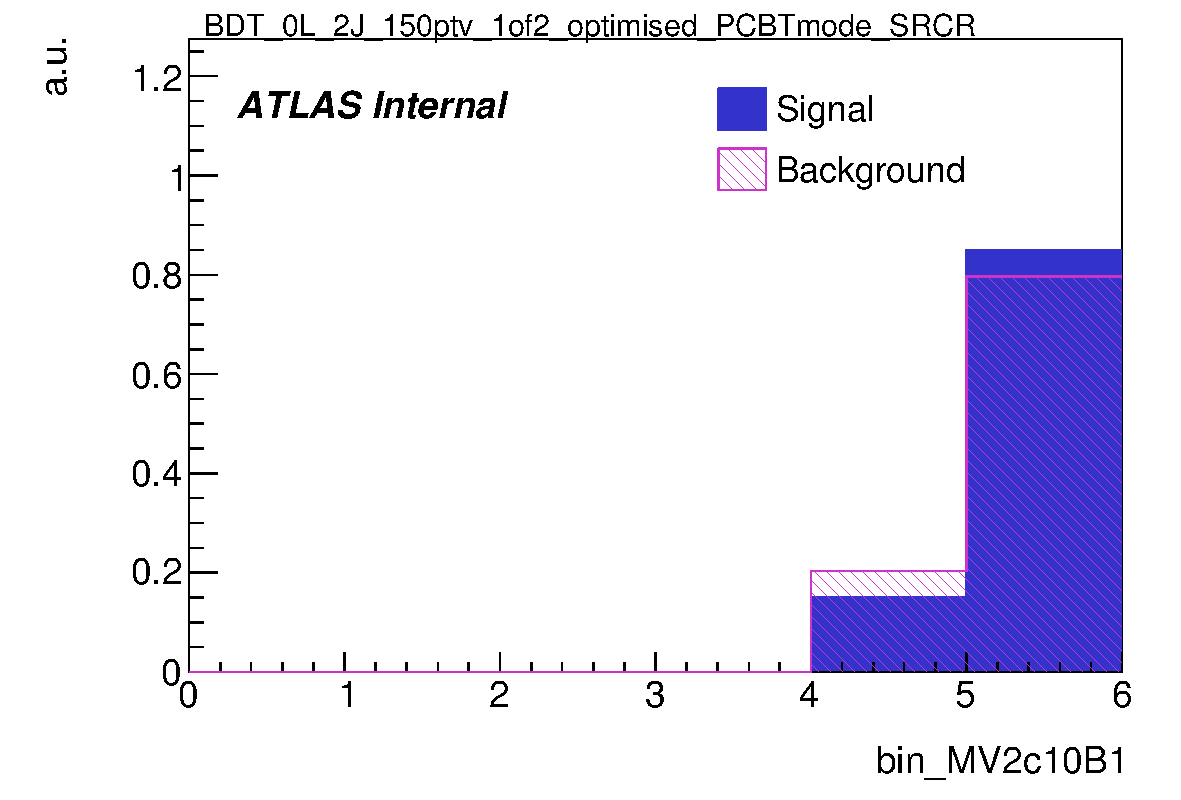
\includegraphics[width=0.33\linewidth]{0-lep-mva/Distr_SignalBackground_bin_MV2c10B1_BDT_0L_2J_150ptv_1of2_optimised_PCBTmode_SRCR-eps-converted-to}}
    \subfloat[]{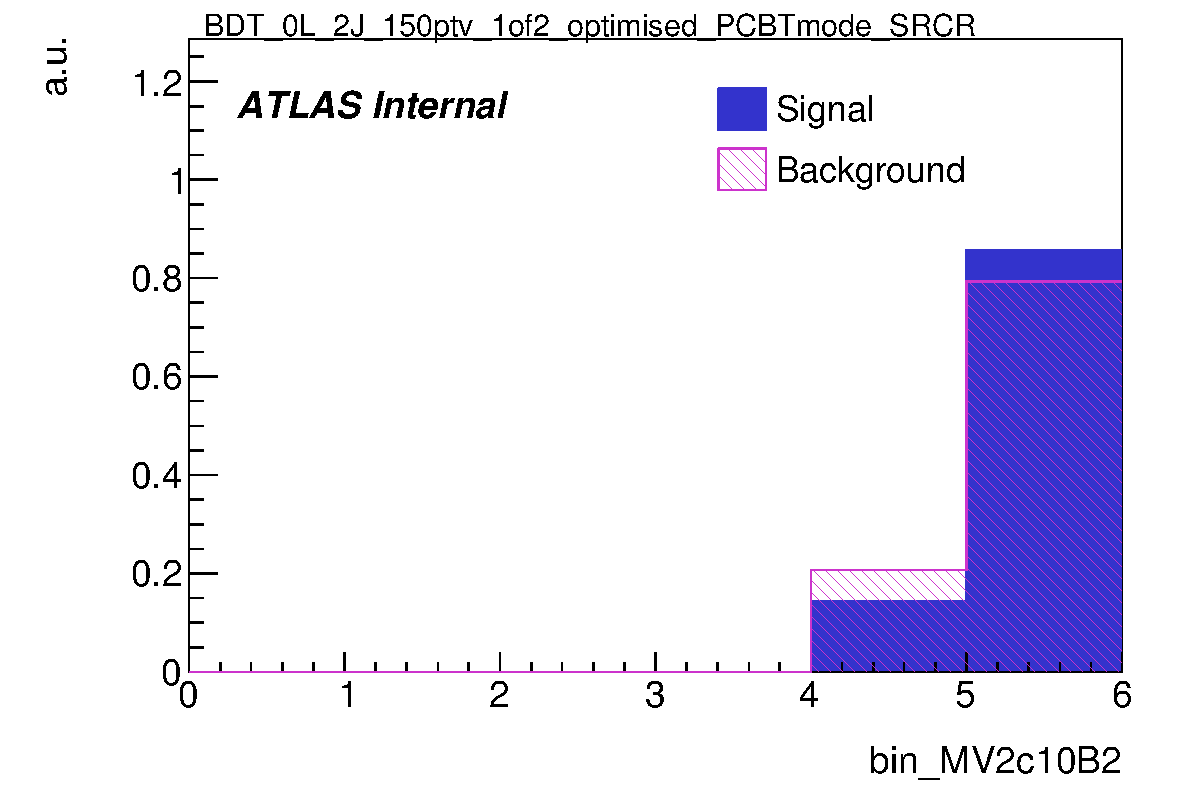
\includegraphics[width=0.33\linewidth]{0-lep-mva/Distr_SignalBackground_bin_MV2c10B2_BDT_0L_2J_150ptv_1of2_optimised_PCBTmode_SRCR-eps-converted-to}}
     \subfloat[]{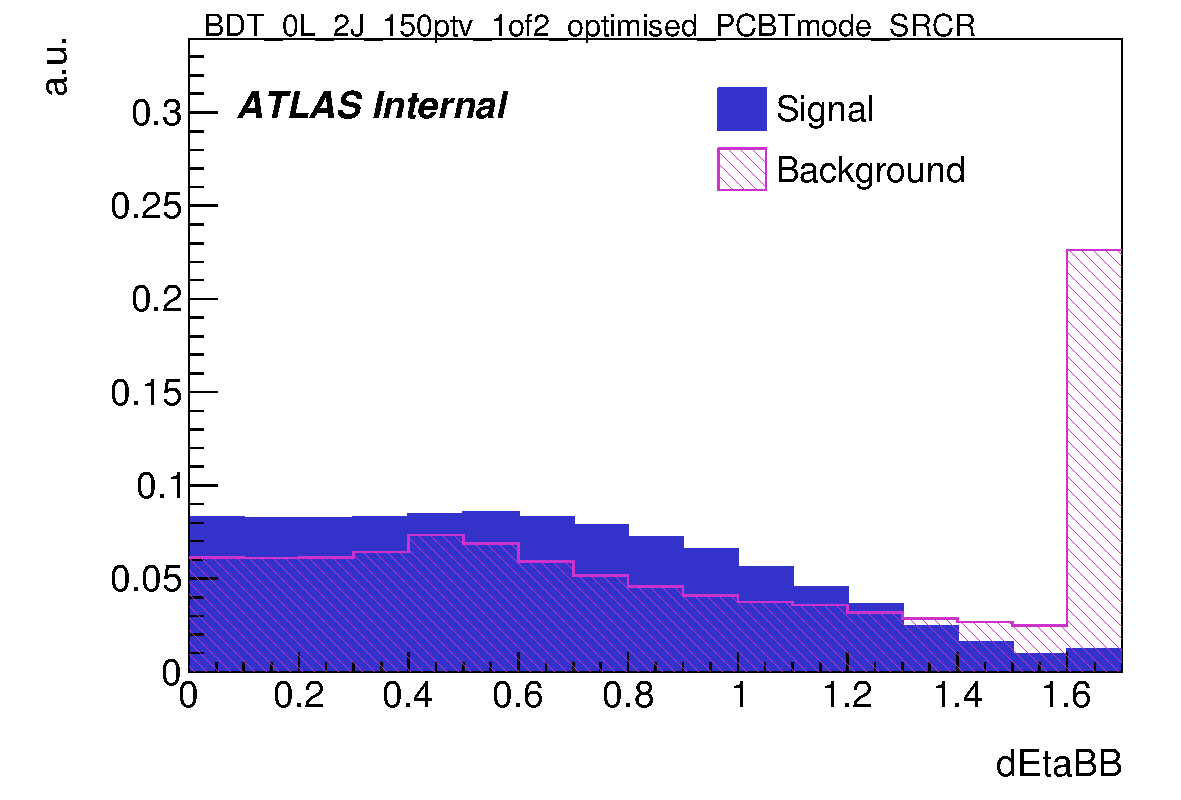
\includegraphics[width=0.33\linewidth]{0-lep-mva/Distr_SignalBackground_dEtaBB_BDT_0L_2J_150ptv_1of2_optimised_PCBTmode_SRCR-eps-converted-to}}\\
    \subfloat[]{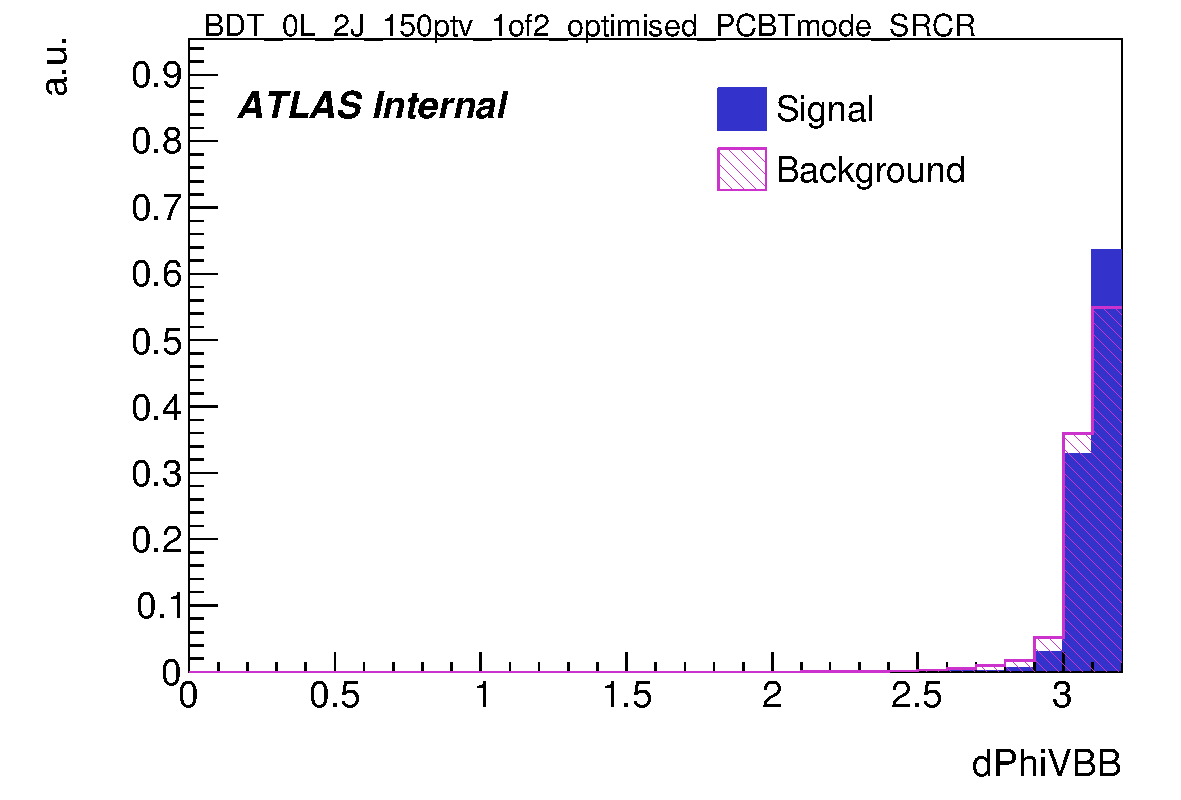
\includegraphics[width=0.33\linewidth]{0-lep-mva/Distr_SignalBackground_dPhiVBB_BDT_0L_2J_150ptv_1of2_optimised_PCBTmode_SRCR-eps-converted-to}}
    \subfloat[]{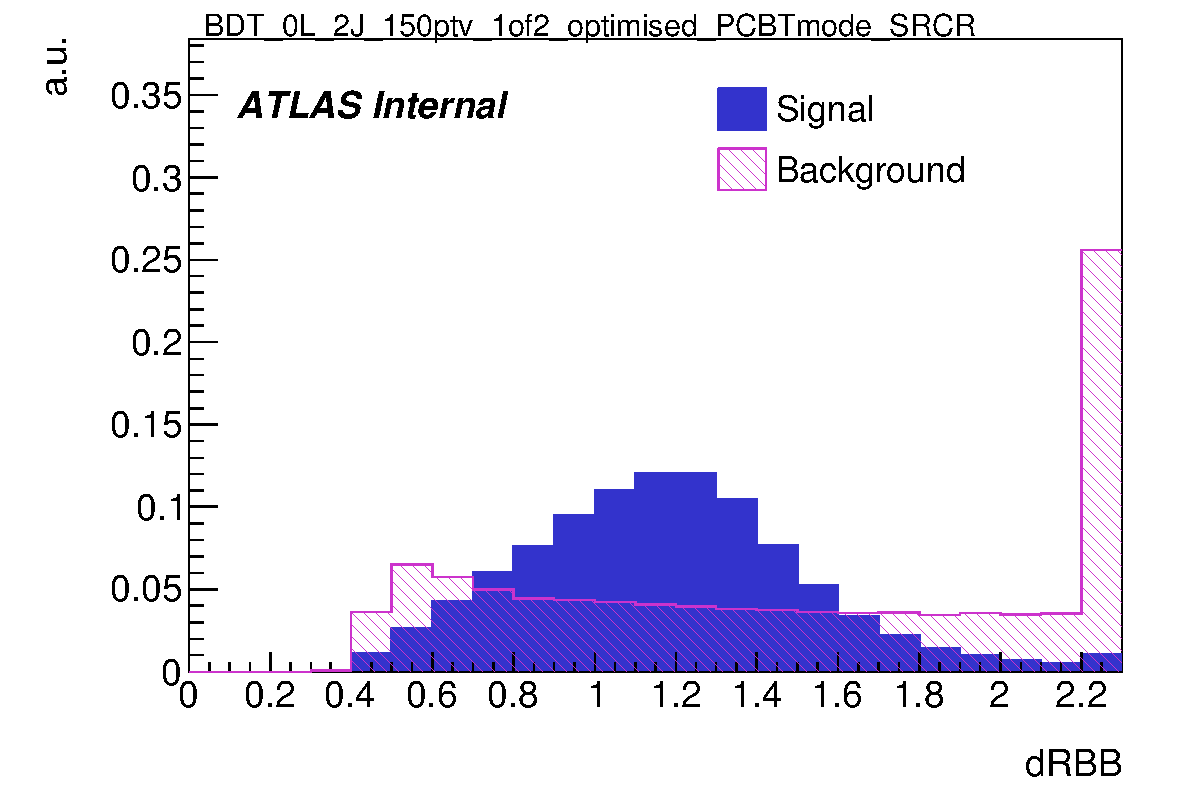
\includegraphics[width=0.33\linewidth]{0-lep-mva/Distr_SignalBackground_dRBB_BDT_0L_2J_150ptv_1of2_optimised_PCBTmode_SRCR-eps-converted-to}}
     \subfloat[]{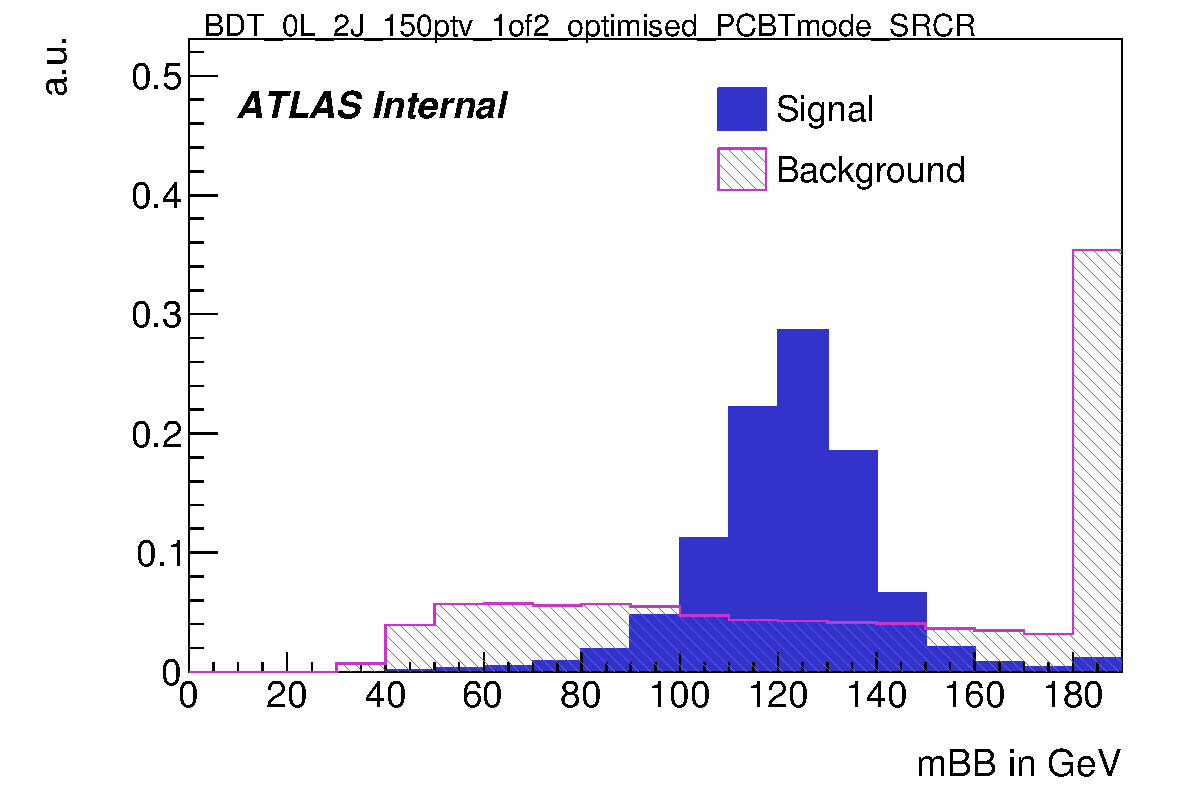
\includegraphics[width=0.33\linewidth]{0-lep-mva/Distr_SignalBackground_mBB_BDT_0L_2J_150ptv_1of2_optimised_PCBTmode_SRCR-eps-converted-to}}\\
    \subfloat[]{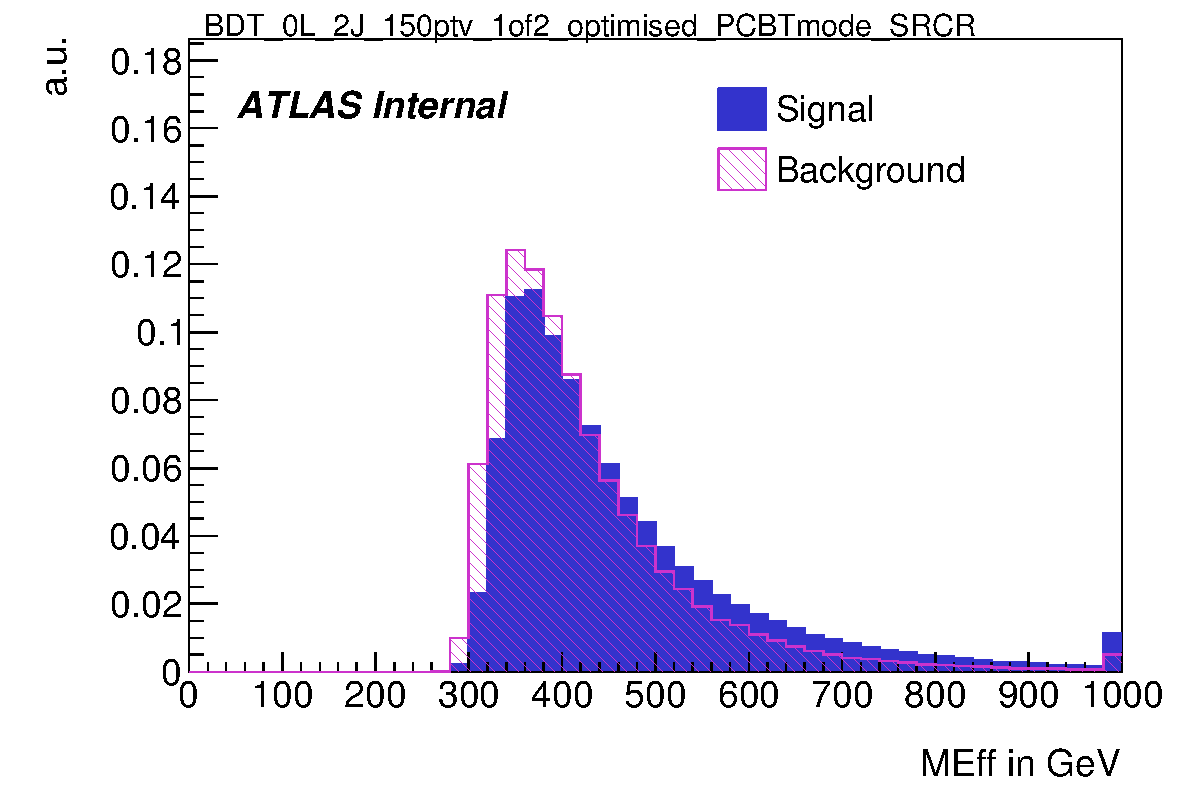
\includegraphics[width=0.33\linewidth]{0-lep-mva/Distr_SignalBackground_MEff_BDT_0L_2J_150ptv_1of2_optimised_PCBTmode_SRCR-eps-converted-to}}
     \subfloat[]{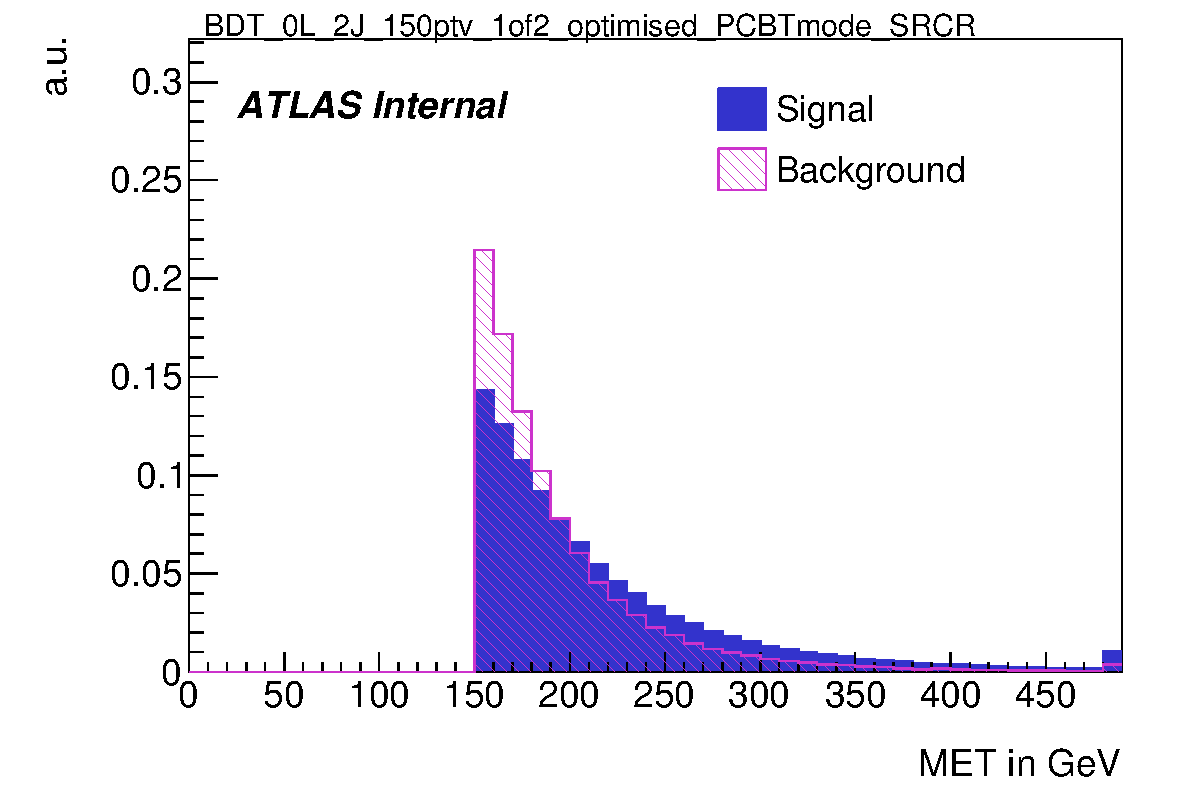
\includegraphics[width=0.33\linewidth]{0-lep-mva/Distr_SignalBackground_MET_BDT_0L_2J_150ptv_1of2_optimised_PCBTmode_SRCR-eps-converted-to}}          
    \subfloat[]{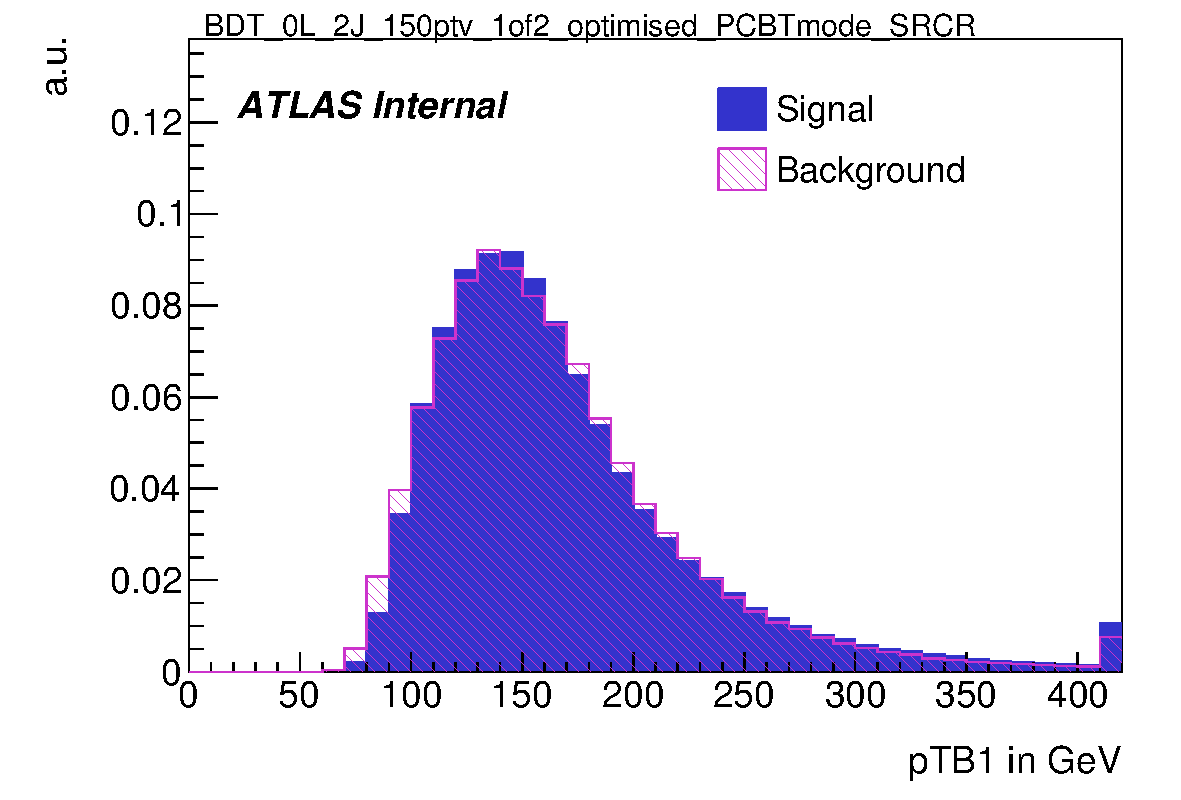
\includegraphics[width=0.33\linewidth]{0-lep-mva/Distr_SignalBackground_pTB1_BDT_0L_2J_150ptv_1of2_optimised_PCBTmode_SRCR-eps-converted-to}} \\
    \subfloat[]{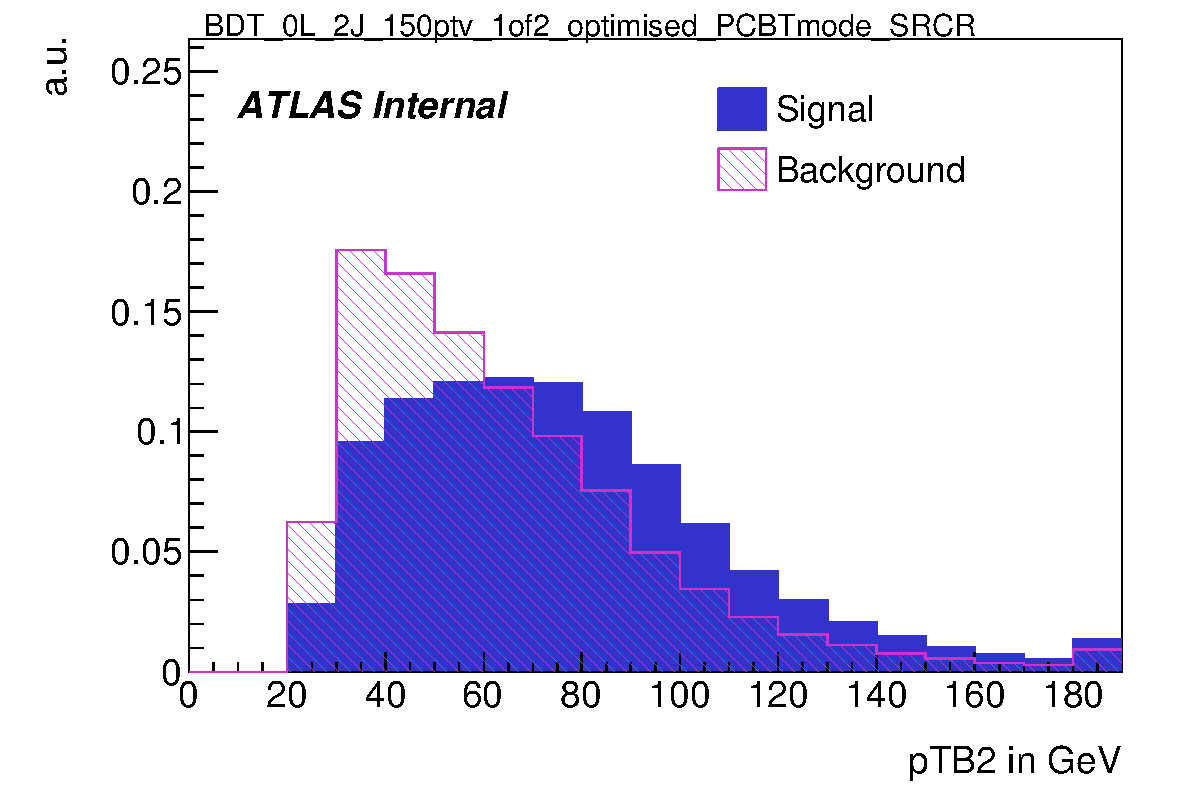
\includegraphics[width=0.33\linewidth]{0-lep-mva/Distr_SignalBackground_pTB2_BDT_0L_2J_150ptv_1of2_optimised_PCBTmode_SRCR-eps-converted-to}}   
    \subfloat[]{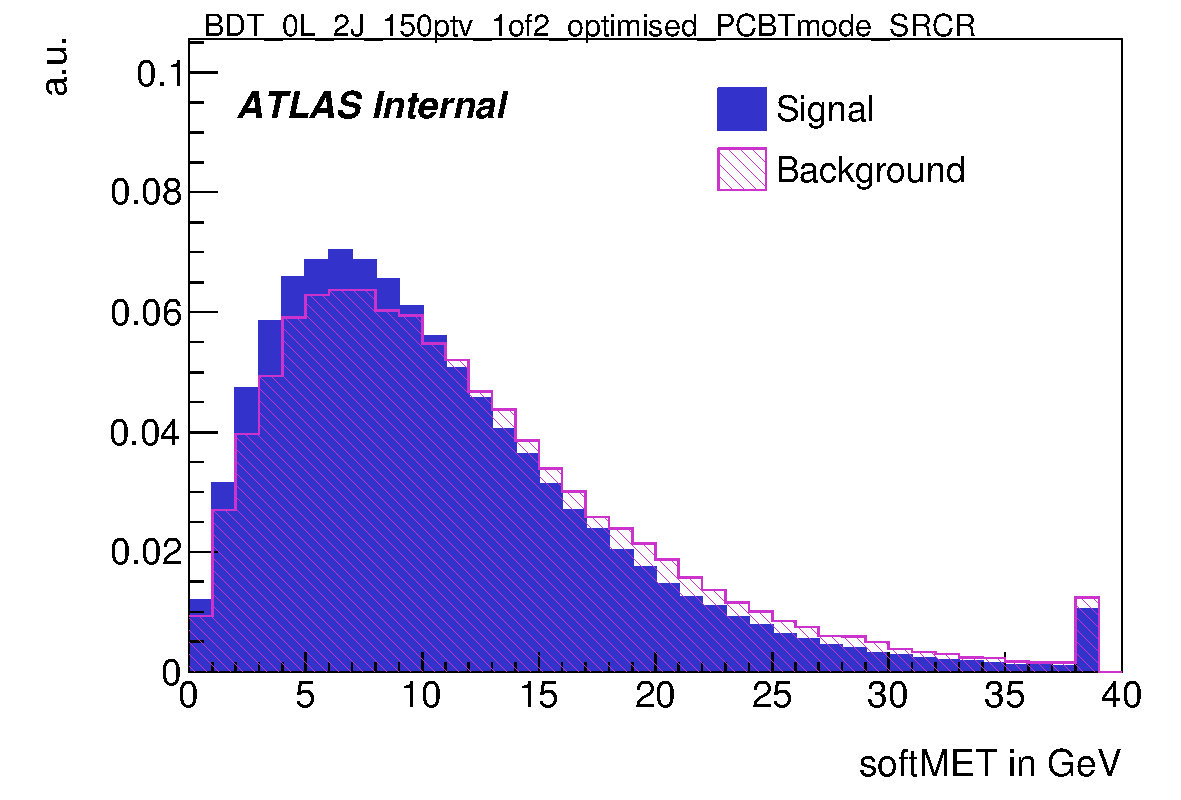
\includegraphics[width=0.33\linewidth]{0-lep-mva/Distr_SignalBackground_softMET_BDT_0L_2J_150ptv_1of2_optimised_PCBTmode_SRCR-eps-converted-to}}\\    
    \end{tabular}
    \caption[Inputs to the multi-variate analysis in the 0--lepton 2--jet
    region.]{Inputs to the multi-variate analysis in the 0--lepton 2--jet
      region. Signal events are shown in blue and background events are shown in
      red. The signal and background histograms have been normalised to the same
      area. The distributions only include events with $E_T^{\text{miss}}$ > 150
      \GeV.}
    \label{fig:bdtinputs-0lep}
\end{figure}

 \begin{figure}[htbp]
  \centering
  \begin{tabular}{cccc}
    \subfloat[]{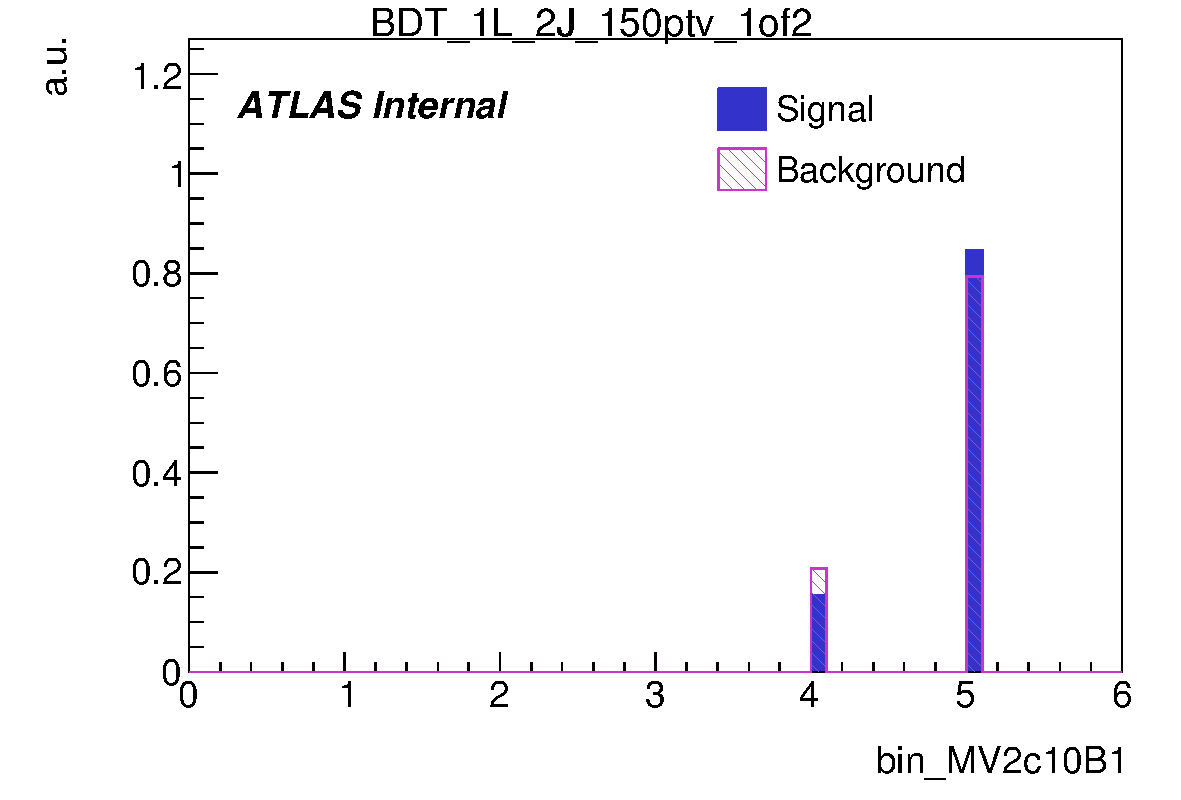
\includegraphics[width=0.3\linewidth]{1-lep-mva/Distr_SignalBackground_bin_MV2c10B1_BDT_1L_2J_150ptv_1of2-eps-converted-to}}
    \subfloat[]{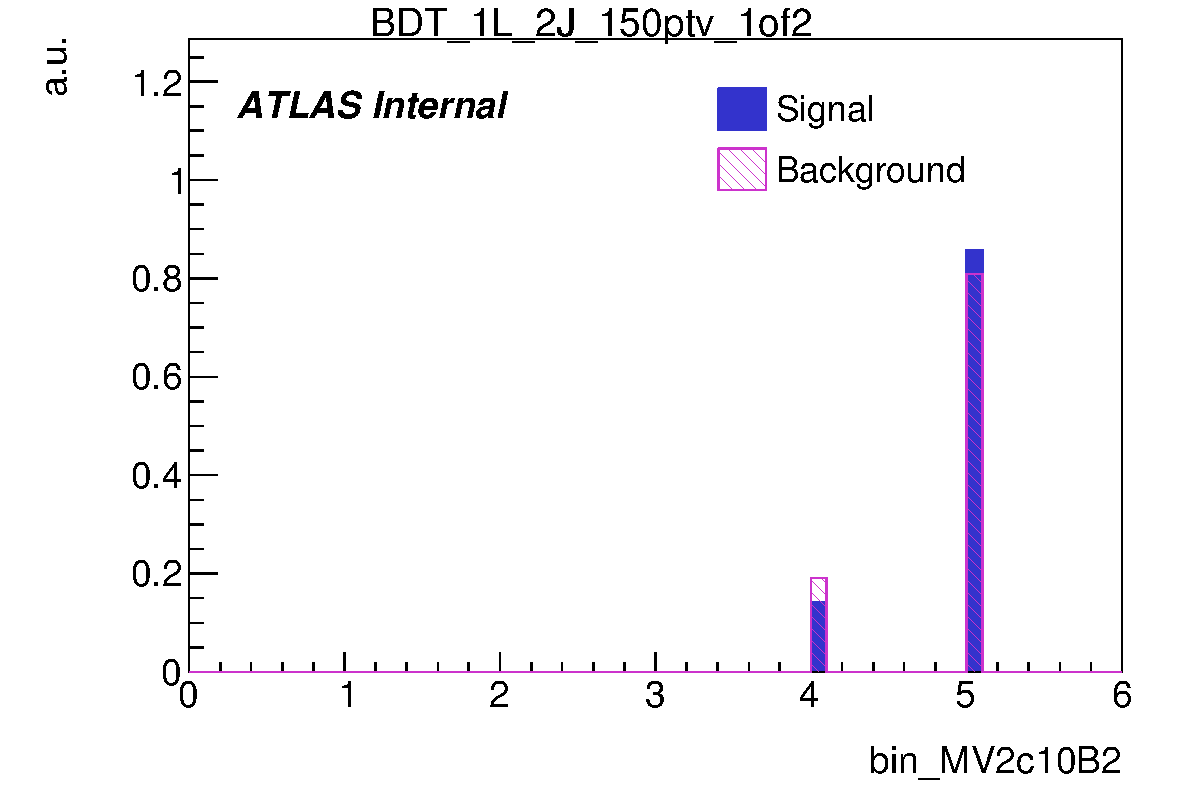
\includegraphics[width=0.3\linewidth]{1-lep-mva/Distr_SignalBackground_bin_MV2c10B2_BDT_1L_2J_150ptv_1of2-eps-converted-to}}
     \subfloat[]{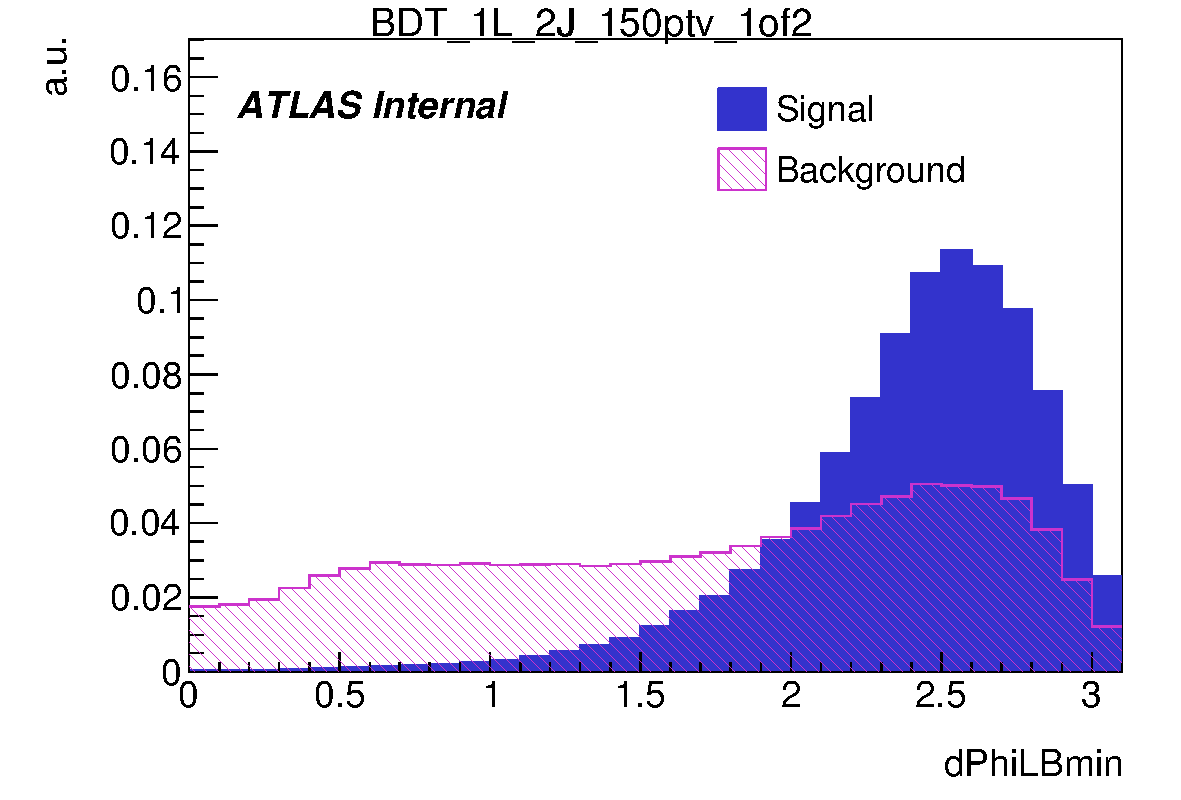
\includegraphics[width=0.3\linewidth]{1-lep-mva/Distr_SignalBackground_dPhiLBmin_BDT_1L_2J_150ptv_1of2-eps-converted-to}}\\
    \subfloat[]{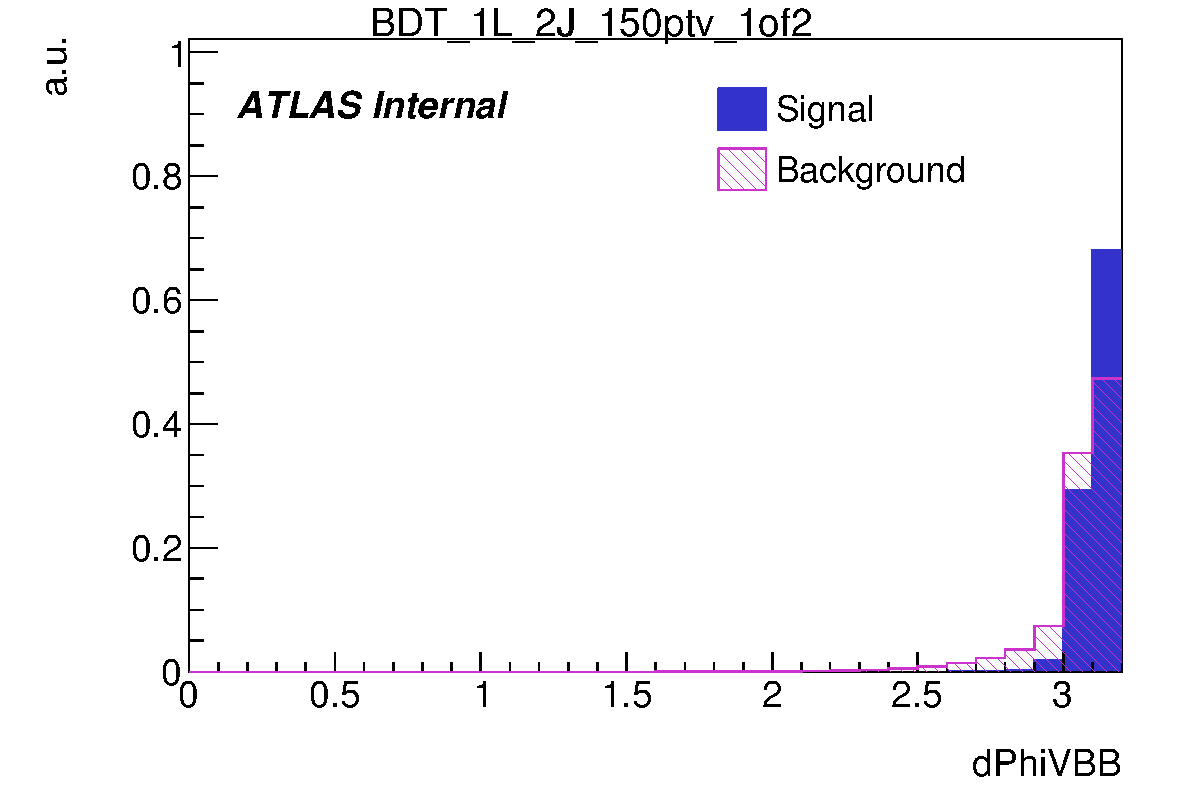
\includegraphics[width=0.3\linewidth]{1-lep-mva/Distr_SignalBackground_dPhiVBB_BDT_1L_2J_150ptv_1of2-eps-converted-to}}
    \subfloat[]{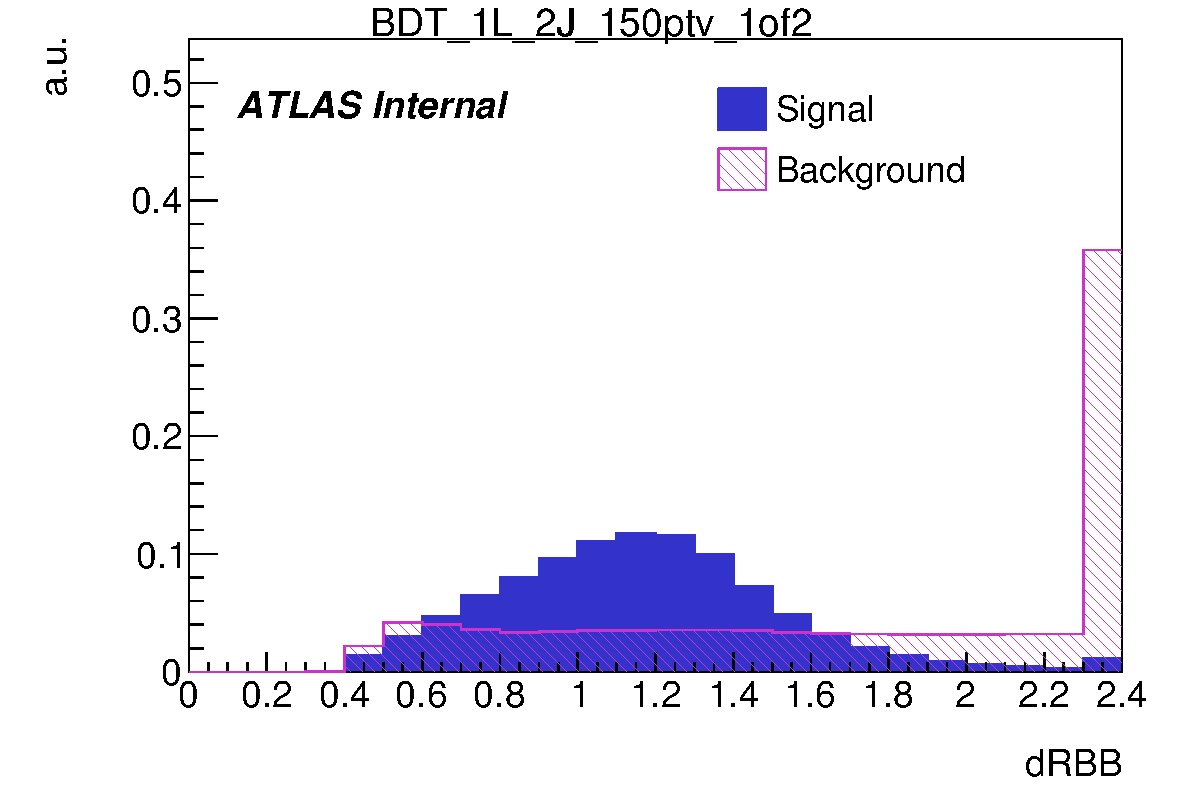
\includegraphics[width=0.3\linewidth]{1-lep-mva/Distr_SignalBackground_dRBB_BDT_1L_2J_150ptv_1of2-eps-converted-to}}
     \subfloat[]{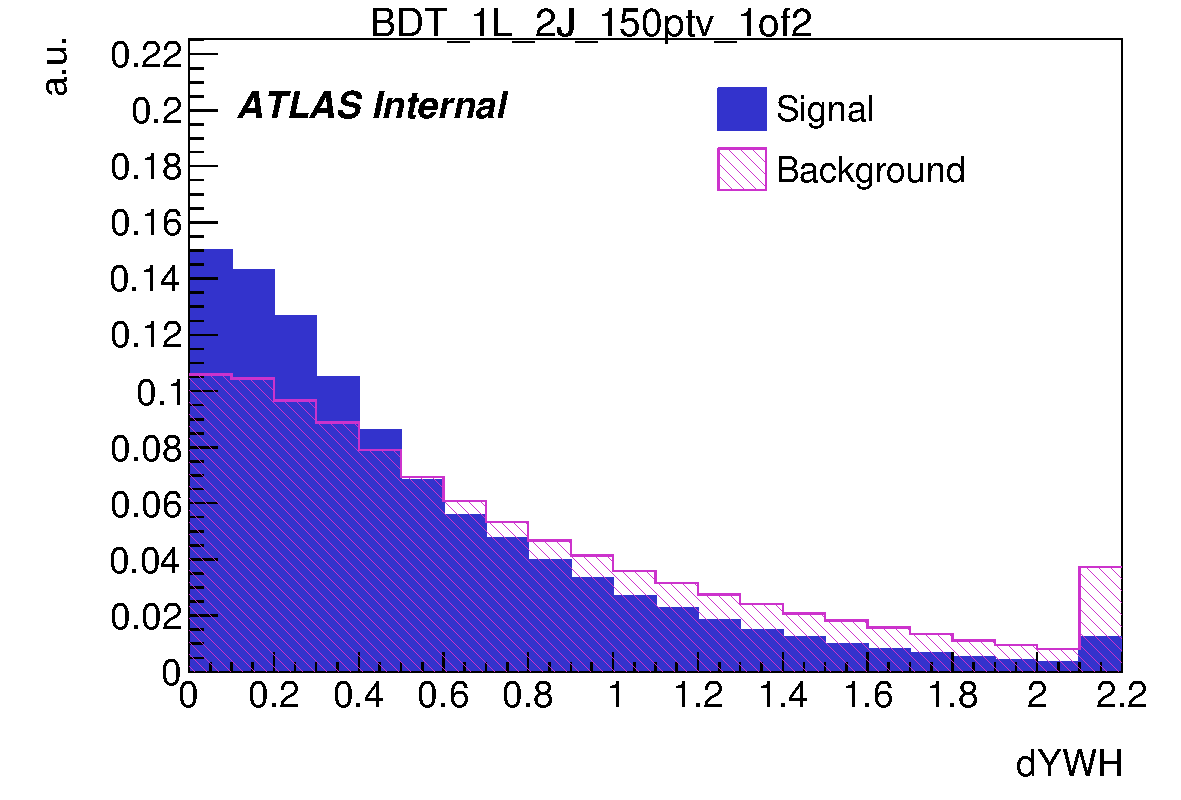
\includegraphics[width=0.3\linewidth]{1-lep-mva/Distr_SignalBackground_dYWH_BDT_1L_2J_150ptv_1of2-eps-converted-to}}\\
    \subfloat[]{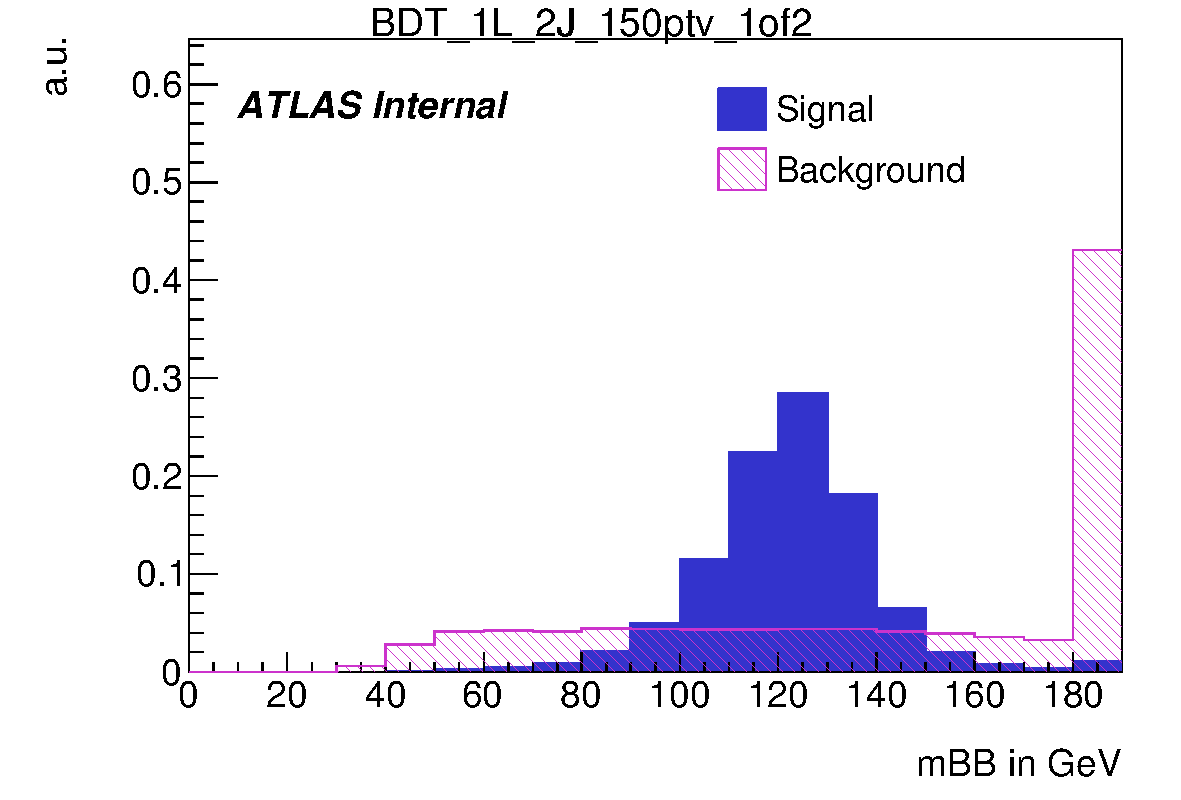
\includegraphics[width=0.3\linewidth]{1-lep-mva/Distr_SignalBackground_mBB_BDT_1L_2J_150ptv_1of2-eps-converted-to}}
     \subfloat[]{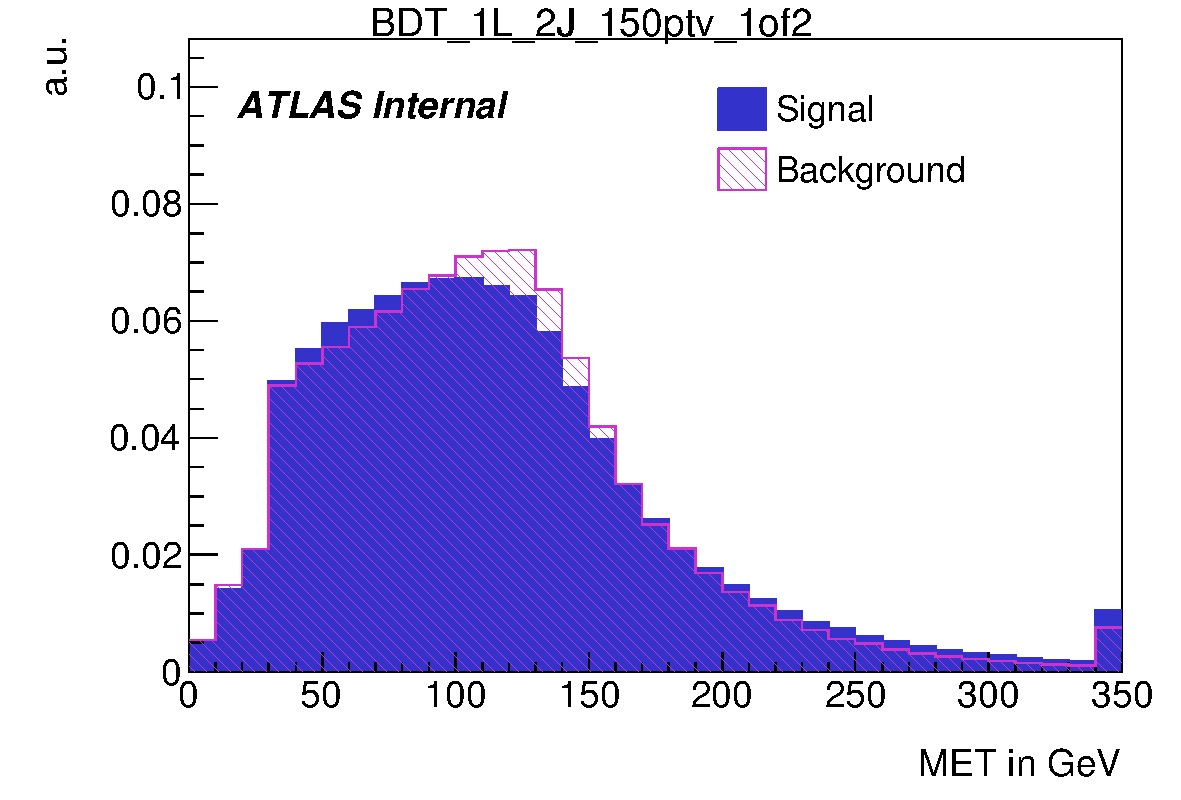
\includegraphics[width=0.3\linewidth]{1-lep-mva/Distr_SignalBackground_MET_BDT_1L_2J_150ptv_1of2-eps-converted-to}}          
    \subfloat[]{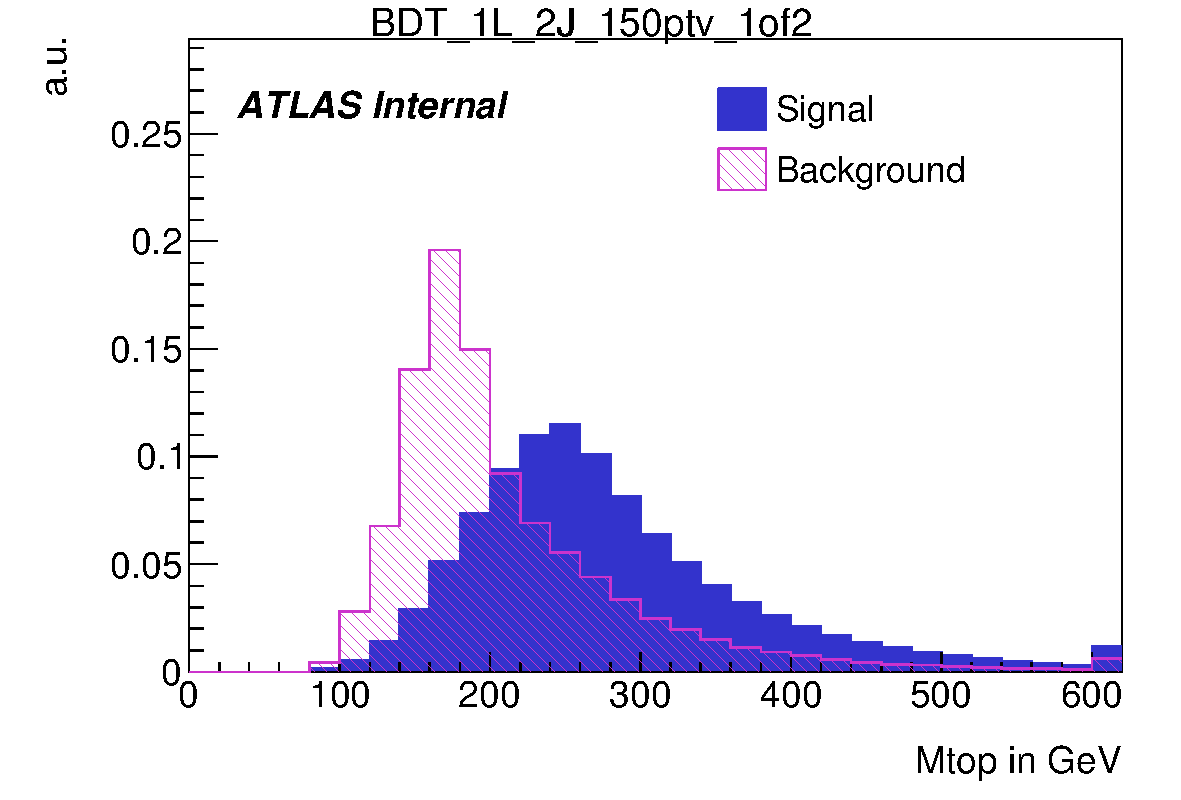
\includegraphics[width=0.3\linewidth]{1-lep-mva/Distr_SignalBackground_Mtop_BDT_1L_2J_150ptv_1of2-eps-converted-to}} \\
    \subfloat[]{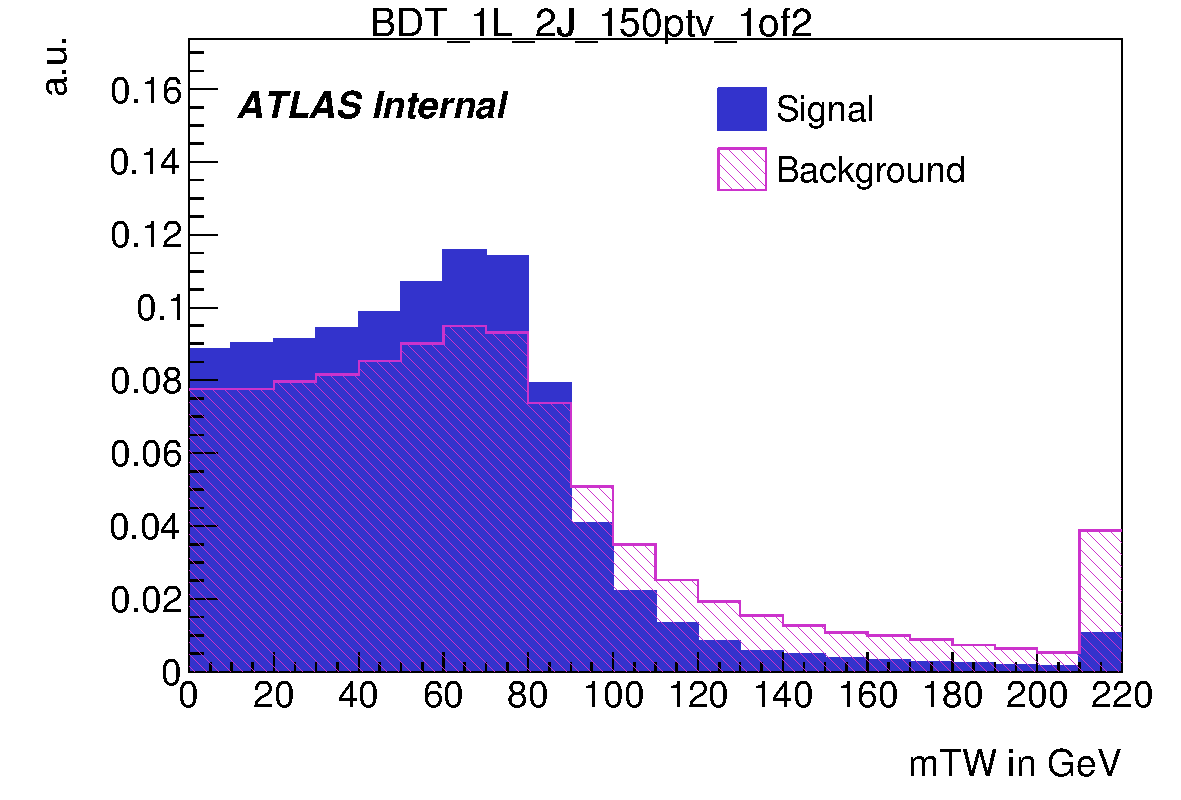
\includegraphics[width=0.3\linewidth]{1-lep-mva/Distr_SignalBackground_mTW_BDT_1L_2J_150ptv_1of2-eps-converted-to}}   
    \subfloat[]{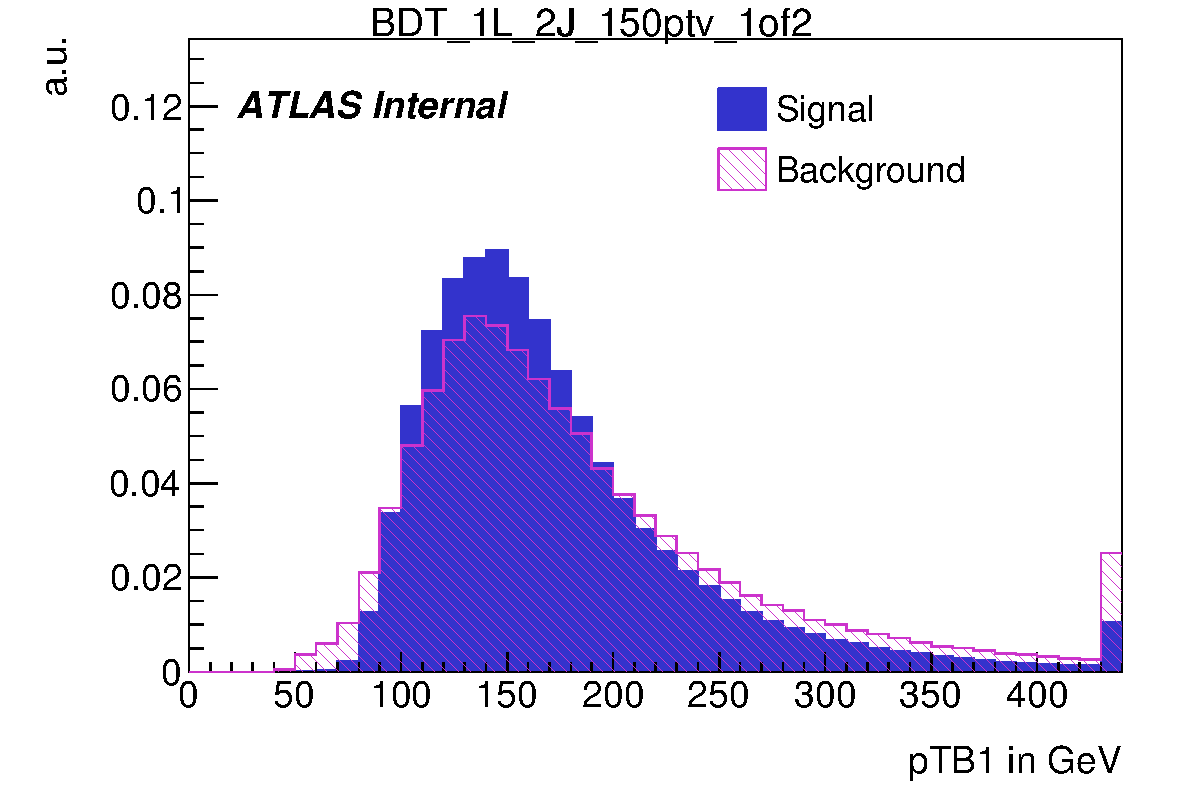
\includegraphics[width=0.3\linewidth]{1-lep-mva/Distr_SignalBackground_pTB1_BDT_1L_2J_150ptv_1of2-eps-converted-to}}
    \subfloat[]{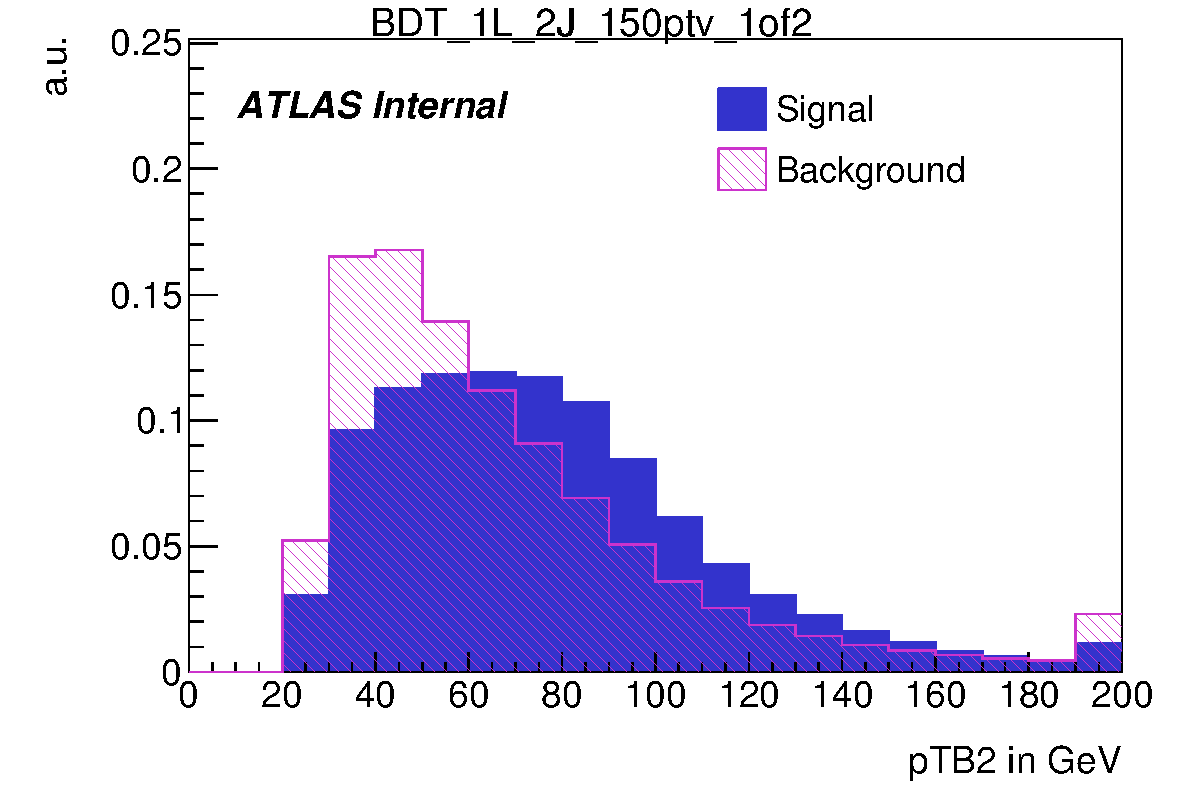
\includegraphics[width=0.3\linewidth]{1-lep-mva/Distr_SignalBackground_pTB2_BDT_1L_2J_150ptv_1of2-eps-converted-to}}\\   
    \subfloat[]{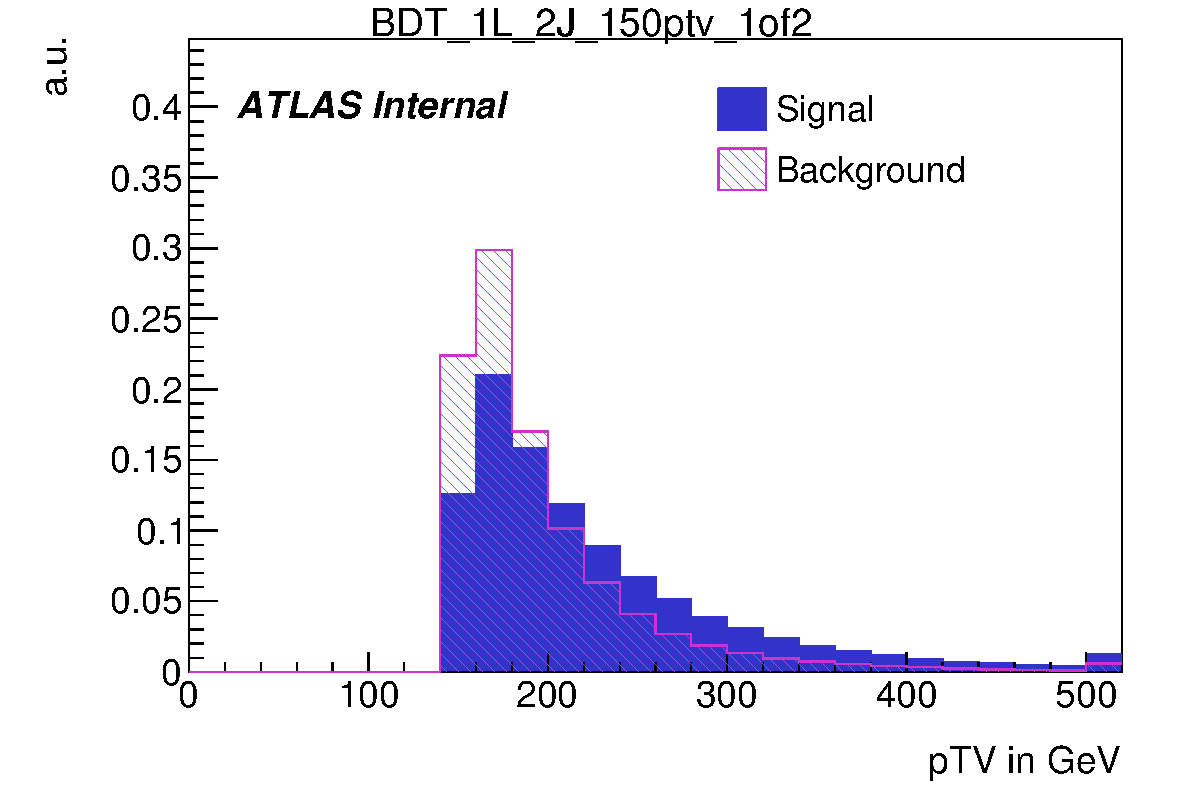
\includegraphics[width=0.3\linewidth]{1-lep-mva/Distr_SignalBackground_pTV_BDT_1L_2J_150ptv_1of2-eps-converted-to}} 
    \end{tabular}
    \caption[Inputs to the multi-variate analysis in the 1--lepton 2--jet
    region.]{Inputs to the multi-variate analysis in the 1--lepton 2--jet
      region. Signal events are shown in blue and background events are shown in
      red. The signal and background histograms have been normalised to the same
      area.The distributions only include events with $p_T^{W}$ > 150
      \GeV.}
    \label{fig:bdtinputs-1lep}
\end{figure}

 \begin{figure}[htbp]
  \centering
  \begin{tabular}{cccc}
    \subfloat[]{\includegraphics[width=0.33\linewidth]{2-lep-mva/Distr_SignalBackground_cosThetaLep_BDT_2L_2J_150ptv_1of2_optimised_PCBTmode_SRCR_extensions-eps-converted-to}}
    \subfloat[]{\includegraphics[width=0.33\linewidth]{2-lep-mva/Distr_SignalBackground_dEtaVBB_BDT_2L_2J_150ptv_1of2_optimised_PCBTmode_SRCR_extensions-eps-converted-to}}
     \subfloat[]{\includegraphics[width=0.33\linewidth]{2-lep-mva/Distr_SignalBackground_dPhiVBB_BDT_2L_2J_150ptv_1of2_optimised_PCBTmode_SRCR_extensions-eps-converted-to}}\\
    \subfloat[]{\includegraphics[width=0.33\linewidth]{2-lep-mva/Distr_SignalBackground_dRBB_BDT_2L_2J_150ptv_1of2_optimised_PCBTmode_SRCR_extensions-eps-converted-to}}
    \subfloat[]{\includegraphics[width=0.33\linewidth]{2-lep-mva/Distr_SignalBackground_mBB_BDT_2L_2J_150ptv_1of2_optimised_PCBTmode_SRCR_extensions-eps-converted-to}}
     \subfloat[]{\includegraphics[width=0.33\linewidth]{2-lep-mva/Distr_SignalBackground_METSig_BDT_2L_2J_150ptv_1of2_optimised_PCBTmode_SRCR_extensions-eps-converted-to}}\\
    \subfloat[]{\includegraphics[width=0.33\linewidth]{2-lep-mva/Distr_SignalBackground_mLL_BDT_2L_2J_150ptv_1of2_optimised_PCBTmode_SRCR_extensions-eps-converted-to}}
     \subfloat[]{\includegraphics[width=0.33\linewidth]{2-lep-mva/Distr_SignalBackground_pTB1_BDT_2L_2J_150ptv_1of2_optimised_PCBTmode_SRCR_extensions-eps-converted-to}}          
    \subfloat[]{\includegraphics[width=0.33\linewidth]{2-lep-mva/Distr_SignalBackground_pTB2_BDT_2L_2J_150ptv_1of2_optimised_PCBTmode_SRCR_extensions-eps-converted-to}} \\
    \subfloat[]{\includegraphics[width=0.33\linewidth]{2-lep-mva/Distr_SignalBackground_pTV_BDT_2L_2J_150ptv_1of2_optimised_PCBTmode_SRCR_extensions-eps-converted-to}}   
    \end{tabular}
    \caption[Inputs to the multi-variate analysis in the 2--lepton 2--jet
    region.]{Inputs to the multi-variate analysis in the 2--lepton 2--jet
      region. Signal events are shown in blue and background events are shown in
      red. The signal and background histograms have been normalised to the same
      area.The distributions only include events with $p_T^{Z}$ > 150
      \GeV.}
    \label{fig:bdtinputs-2lep}
\end{figure}


  
- What regions is it trained on?

- What is the performance like?

- Transformation

\section{Pre-fit plots}
\label{sec:prefit}

This section shows the pre-fit distributions of the Monte-Carlo prediction
versus the data in every analysis region that enters into the profile-likelihood
fit. Figures~\ref{fig:0lep-2jet-prefit},~\ref{fig:0lep-3jet-prefit} show the
distributions in the 0--lepton channel in the 2--jet and 3--jet regions
respectively. Figures~\ref{fig:1lep-2jet-prefit},~\ref{fig:1lep-3jet-prefit} show the
distributions in the 1--lepton channel in the 2--jet and 3--jet regions
respectively. Figures~\ref{fig:2lep-2jet-prefit},~\ref{fig:2lep-3pjet-prefit} show the
distributions in the 2--lepton channel in the 2--jet and 3+--jet regions
respectively.
\begin{figure}
  \centering
  \begin{tabular}{cc}
    % top row
    \includegraphics[width=.49\textwidth]{final_fit_mva/prefit/Region_BMax250_BMin150_Y6051_DCRHigh_T2_L0_distMET_J2_Prefit}%
    & \includegraphics[width=.49\textwidth]{final_fit_mva/prefit/Region_BMin250_Y6051_DCRHigh_T2_L0_distMET_J2_Prefit} \\

    % middle row
    \includegraphics[width=.49\textwidth]{final_fit_mva/prefit/Region_BMax250_BMin150_Y6051_DSR_T2_L0_distmva_J2_Prefit}%
    & \includegraphics[width=.49\textwidth]{final_fit_mva/prefit/Region_BMin250_Y6051_DSR_T2_L0_distmva_J2_Prefit} \\

    % bottom row
    \includegraphics[width=.49\textwidth]{final_fit_mva/prefit/Region_BMax250_BMin150_Y6051_DCRLow_T2_L0_distMET_J2_Prefit}%
    & \includegraphics[width=.49\textwidth]{final_fit_mva/prefit/Region_BMin250_Y6051_DCRLow_T2_L0_distMET_J2_Prefit} \\
  \end{tabular}
  \caption{Pre-fit distributions in the 0--lepton channel in the 2--jet region.}
  \label{fig:0lep-2jet-prefit}
\end{figure}
\begin{figure}
  \centering
  \begin{tabular}{cc}
    % top row
    \includegraphics[width=.3\textwidth]{final_fit_mva/prefit/Region_BMax250_BMin150_Y6051_DCRHigh_T2_L0_distMET_J3_Prefit}%
    & \includegraphics[width=.3\textwidth]{final_fit_mva/prefit/Region_BMin250_Y6051_DCRHigh_T2_L0_distMET_J3_Prefit} \\

    % middle row
    \includegraphics[width=.3\textwidth]{final_fit_mva/prefit/Region_BMax250_BMin150_Y6051_DSR_T2_L0_distmva_J3_Prefit}%
    & \includegraphics[width=.3\textwidth]{final_fit_mva/prefit/Region_BMin250_Y6051_DSR_T2_L0_distmva_J3_Prefit} \\

    % bottom row
    \includegraphics[width=.3\textwidth]{final_fit_mva/prefit/Region_BMax250_BMin150_Y6051_DCRLow_T2_L0_distMET_J3_Prefit}%
    & \includegraphics[width=.3\textwidth]{final_fit_mva/prefit/Region_BMin250_Y6051_DCRLow_T2_L0_distMET_J3_Prefit} \\
  \end{tabular}
  \caption{Pre-fit distributions in the 0 lepton 3 jet channel.}
\end{figure}
\begin{figure}
  \centering
  \begin{tabular}{cc}
    % top row
    \includegraphics[width=.3\textwidth]{final_fit_mva/prefit/Region_BMax250_BMin150_Y6051_DCRHigh_T2_L1_distpTV_J2_Prefit}%
    & \includegraphics[width=.3\textwidth]{final_fit_mva/prefit/Region_BMin250_Y6051_DCRHigh_T2_L1_distpTV_J2_Prefit} \\

    % middle row
    \includegraphics[width=.3\textwidth]{final_fit_mva/prefit/Region_BMax250_BMin150_Y6051_DSR_T2_L1_distmva_J2_Prefit}%
    & \includegraphics[width=.3\textwidth]{final_fit_mva/prefit/Region_BMin250_Y6051_DSR_T2_L1_distmva_J2_Prefit} \\

    % bottom row
    \includegraphics[width=.3\textwidth]{final_fit_mva/prefit/Region_BMax250_BMin150_Y6051_DCRLow_T2_L1_distpTV_J2_Prefit}%
    & \includegraphics[width=.3\textwidth]{final_fit_mva/prefit/Region_BMin250_Y6051_DCRLow_T2_L1_distpTV_J2_Prefit} \\
  \end{tabular}
  \caption{Pre-fit distributions in the 1 lepton 2 jet channel.}
\end{figure}
\begin{figure}
  \centering
  \begin{tabular}{cc}
    % top row
    \includegraphics[width=.3\textwidth]{final_fit_mva/prefit/Region_BMax250_BMin150_Y6051_DCRHigh_T2_L1_distpTV_J3_Prefit}%
    & \includegraphics[width=.3\textwidth]{final_fit_mva/prefit/Region_BMin250_Y6051_DCRHigh_T2_L1_distpTV_J3_Prefit} \\

    % middle row
    \includegraphics[width=.3\textwidth]{final_fit_mva/prefit/Region_BMax250_BMin150_Y6051_DSR_T2_L1_distmva_J3_Prefit}%
    & \includegraphics[width=.3\textwidth]{final_fit_mva/prefit/Region_BMin250_Y6051_DSR_T2_L1_distmva_J3_Prefit} \\

    % bottom row
    \includegraphics[width=.3\textwidth]{final_fit_mva/prefit/Region_BMax250_BMin150_Y6051_DCRLow_T2_L1_distpTV_J3_Prefit}%
    & \includegraphics[width=.3\textwidth]{final_fit_mva/prefit/Region_BMin250_Y6051_DCRLow_T2_L1_distpTV_J3_Prefit} \\
  \end{tabular}
  \caption{Pre-fit distributions in the 1 lepton 3 jet channel.}
\end{figure}
\begin{figure}
  \centering
  \begin{tabular}{cc}
    % top row
    \includegraphics[width=.33\textwidth]{final_fit_mva/prefit/Region_BMax150_BMin75_Y6051_DCRHigh_T2_L2_distpTV_J2_Prefit}%
    \includegraphics[width=.33\textwidth]{final_fit_mva/prefit/Region_BMax250_BMin150_Y6051_DCRHigh_T2_L2_distpTV_J2_Prefit}%
    & \includegraphics[width=.33\textwidth]{final_fit_mva/prefit/Region_BMin250_Y6051_DCRHigh_T2_L2_distpTV_J2_Prefit} \\

    % middle row
    \includegraphics[width=.33\textwidth]{final_fit_mva/prefit/Region_BMax150_BMin75_Y6051_DSR_T2_L2_distmva_J2_Prefit}%
    \includegraphics[width=.33\textwidth]{final_fit_mva/prefit/Region_BMax250_BMin150_Y6051_DSR_T2_L2_distmva_J2_Prefit}%
    & \includegraphics[width=.33\textwidth]{final_fit_mva/prefit/Region_BMin250_Y6051_DSR_T2_L2_distmva_J2_Prefit} \\

    % bottom row
    \includegraphics[width=.33\textwidth]{final_fit_mva/prefit/Region_BMax150_BMin75_Y6051_DCRLow_T2_L2_distpTV_J2_Prefit}%
    \includegraphics[width=.33\textwidth]{final_fit_mva/prefit/Region_BMax250_BMin150_Y6051_DCRLow_T2_L2_distpTV_J2_Prefit}%
    & \includegraphics[width=.33\textwidth]{final_fit_mva/prefit/Region_BMin250_Y6051_DCRLow_T2_L2_distpTV_J2_Prefit} \\
  \end{tabular}
  \caption{Pre-fit distributions in the 2--lepton channel in the  2--jet
    region.}
  \label{fig:2lep-2jet-prefit}
\end{figure}
\begin{figure}
  \centering
  \begin{tabular}{cc}
    % top row
    \includegraphics[width=.3\textwidth]{final_fit_mva/prefit/Region_BMax150_BMin75_incJet1_Y6051_DCRHigh_T2_L2_distpTV_J3_Prefit}%
    \includegraphics[width=.3\textwidth]{final_fit_mva/prefit/Region_BMax250_BMin150_incJet1_Y6051_DCRHigh_T2_L2_distpTV_J3_Prefit}%
    & \includegraphics[width=.3\textwidth]{final_fit_mva/prefit/Region_BMin250_incJet1_Y6051_DCRHigh_T2_L2_distpTV_J3_Prefit} \\

    % middle row
    \includegraphics[width=.3\textwidth]{final_fit_mva/prefit/Region_BMax150_BMin75_incJet1_Y6051_DSR_T2_L2_distmva_J3_Prefit}%
    \includegraphics[width=.3\textwidth]{final_fit_mva/prefit/Region_BMax250_BMin150_incJet1_Y6051_DSR_T2_L2_distmva_J3_Prefit}%
    & \includegraphics[width=.3\textwidth]{final_fit_mva/prefit/Region_BMin250_incJet1_Y6051_DSR_T2_L2_distmva_J3_Prefit} \\

    % bottom row
    \includegraphics[width=.3\textwidth]{final_fit_mva/prefit/Region_BMax150_BMin75_incJet1_Y6051_DCRLow_T2_L2_distpTV_J3_Prefit}%
    \includegraphics[width=.3\textwidth]{final_fit_mva/prefit/Region_BMax250_BMin150_incJet1_Y6051_DCRLow_T2_L2_distpTV_J3_Prefit}%
    & \includegraphics[width=.3\textwidth]{final_fit_mva/prefit/Region_BMin250_incJet1_Y6051_DCRLow_T2_L2_distpTV_J3_Prefit} \\
  \end{tabular}
  \caption{Pre-fit distributions in the 2--lepton channel in the  3+--jet
    region.}
  \label{fig:2lep-3pjet-prefit}
\end{figure}

\section{Analysis Cross-checks}

The final elements of the analysis strategy are a series of cross-checks that
are designed to ensure the methodology is robust. Firstly there is the di-jet
mass fit, also known as the $m_{bb}$ fit. This cross-check is designed to ensure
that the multi-variate analysis has not introduced any biases that have changed
the result so much that is statistically incompatible with a version of the
analysis that does not use the BDT. This cross-check is performed by simply
taking the $m_{bb}$ distribution in place of the BDT distribution in the
profile-likelihood fit.

The second cross-check is a measurement of the diboson process. Diboson final
states arising from proton-proton collisions are well understood and in this
case are being treated as a standard candle~\footnote{A standard candle is an
  astronomical object with a known absolute luminosity that can be used to aid
  astronomical measurements. }. The rationale here is that if the analysis
methodology produces a measurement of the diboson process that is in agreement
with the Standard Model prediction, and therefore existing measurements, then
the methodology itself has not introduced unexpected effects on the result.





\chapter{Systematic Uncertainties}%
\label{ch:systematics}

So far the only errors considered are the random statistical errors on the data
and Monte-Carlo predictions. Systematic errors enter into the analysis in a
large number of places, in this chapter the systematic errors considered in the
analysis are detailed. In general the systematic errors come in one of two
forms, either a shape effect or a normalisation effect. Normalisation effects
alter the number of events in a given sample across the entire sample simply
changing the total number of events. Shape effects change where events lie in a
given distribution causing events to migrate between bins of a histogram, and
potentially across boundaries that are used to define analysis regions described
in~\ref{sec:ana-regions}.

A sub-category of normalisation effect is the acceptance effect which deals with
the normalisation in a particular region or set of regions. The purpose of the
acceptance uncertainties is to account for any mismodelling in the theoretical
prediction of the quantities used to categorise events into regions be it the
leptonic channel, jet multiplicity or an analysis region. Nuisance parameters in
the profile likelihood fit are used to control the acceptance, they are
implemented as Gaussian probability densities whose priors are estimated in
advance. The priors of all of these so called acceptance uncertainties are
calculated using the double ratio
\begin{equation}
  \left. \dfrac{N_{A}^{\text{nominal}}}{N_{B}^{\text{nominal}}} \middle/ \dfrac{N_{A}^{\text{alternative}}}{N_{B}^{\text{alternative}}} \right.,
  \label{eq:acceptance-dr}
\end{equation}
where the formula has been written agnostic of the specific application so
$N_{A}^{nominal}$ is the number of  events in the nominal prediction in some
region or category called $A$ and so on.

Another variant of the normalisation effect are the flavour composition
uncertainties. Rather than impacting the normalisation of an entire background
in terms of how they are categorised in the analysis plots, for example in the
plots in section~\ref{sec:prefit}, they impact the sub-processes split by
flavour of the decay products individually. A heavy flavour process is defined as
one where the two leading jets have flavour (b,~b), (b,~c), (b,~l), or (c,~c),
this categorisation is often written as hf for short for example when
considering all heavy flavour sub-process of the V + jets background one could
write V + hf. Flavour composition uncertainties affect the normalisation of one
of the flavour sub-processes with respect to one of the others, specific details
will follow under the sections relating to the relevant backgrounds.

The rest of this chapter will detail the sources of systematic error broken down
into groups of similar origin. Before breaking down each group of systematic
errors a technique called the Boosted Decision Tree Re-weighting method will be
explained as it used across a number of the different groups. The author's
contributions include the determination of all of the Z + jets systematic
errors, determination of systematic errors relating to the flavour composition
of simulated top process events, and development and testing of the Boosted
Decision Tree Re-weighting method.

\section{Parametrising Variance Due To Shape Uncertainties}
\label{sec:re-weighting}

The predictions entering into the profile-likelihood fit of the analysis can be
written as a probability density $p(\vec{x}|\vec{\theta})$, where $\vec{x} =
[x_{1},..., x_{i}]$ is a vector of observable quantities, with $N$ elements and
$\vec{\theta}$ represents the theoretical parameters of the model. The
parameters may come from the Standard Model theory or phenomenological
considerations that must be taken into account to turn that theory into a usable
prediction.

As described above, shape effects may impact the prediction of a given
Monte-Carlo generator that has a particular set of parameters. The choice of
generator will change the prediction due to different choices made by the
generator creators, including but not limited to, the parton shower model,
hadronisation model and non-perturbative processes. One way to get a handle on
the variance of a particular generator is therefore to literally vary these
choices by picking an alternative generator and drawing a comparison to the
alternative prediction. This method is flawed in ways which will be discussed
but is nonetheless fairly common and often one of the few choices available to
analysers when they are trying to get an idea of what the systematic errors on
the modelling of complex physics processes are. Two such methods of comparison
will be detailed here as they are used in this analysis, they the single
dimension parameterisation described in section~\ref{sec:1D-reweight} and a
multi-dimensional parameterisation described in section~\ref{sec:ND-reweight}.
Following this a hybrid approach which uses both methods will be described in
section~\ref{sec:hybrid-reweight}. These methods are described here in general
and then the specific implementations are discussed later under sections
relevant to the systematic errors they are used to calculate.

\subsection{Single Dimension Parameterisation}
\label{sec:1D-reweight}

The single dimension parameterisation uses the ratio of probability densities
\begin{equation}
  r(\vec{x}) = \frac{p(\vec{x}|\vec{\theta}_{1})}{p(\vec{x}|\vec{\theta}_{0})},
  \label{eq:DensityRatio}
\end{equation}
where the subscripts on $\vec{\theta}$ number different choices of the
parameters which govern the model, for example due to different choice of
generator. Here the subscript 0 denotes the nominal prediction and 1 denotes an
alternative. In order to map the nominal to the alternative it is clear that the
one can multiply $p(\vec{x}|\vec{\theta}_{0})$ by the ratio.

The only way that this calculation is tractable is to consider a single
dimension of the probability density function, specifically a single observable
chosen from the vector $\vec{x}$. The ratio then becomes
\begin{equation}
  r(x_{i}) = \frac{p(x_{i}|\vec{\theta}_{1})}{p(x_{i}|\vec{\theta}_{0})},
  \label{eq:1D-ratio}
\end{equation}
which can in turn be calculated for as many or as few as the elements of
$\vec{x}$ as is desired. It should be noted that when the ratio is calculated
using only a single variable it can still be used to map the $N$ dimensional
nominal prediction to the alternative, however the mapping is only guaranteed to
be successful in the dimension chosen to calculate the ratio and in general
agreement between the two predictions in the other variables can not be relied
upon.

Figure~\ref{fig:1d-rw-illustration} shows a graphical illustration of how this
single dimensional ratio is calculated. In practice the ratio is used to derive
a systematic shape uncertainty by weighting each event in the nominal
prediction as a function of the variable $x_{i}$ whose distribution was used to
calculate the ratio. Limitations on the sample size of each prediction mean that
in practice it is better to smooth the ratio via the use of a parametric fit in
order to mitigate any large statistical fluctuations in a single bin of the
ratio (arising from a large fluctuation in one of the predictions in that bin).
In figure~\ref{fig:1d-rw-illustration} the parametric fit is represented by the
solid line in the ratio.
\begin{figure}[t]
  \centering
  \includegraphics[width=.65\linewidth]{placeholder}
  \caption[An illustration of the N--dimensional parametrisation of a shape
  difference between two datasets.]{Illustration of the calculation of a ratio
    of probability densities in a single dimension.}
  \label{fig:1d-rw-illustration}
\end{figure}

\subsection{$N$-dimensional Parametrisation}
\label{sec:ND-reweight}

As already alluded to in the previous section there are issues with the
parametrisation in a single dimension. Not only is the mapping only guaranteed
to work in a single dimension but if the technique is applied sequentially on
one variable after another the mapping from the first step can be undone by the
second. That is to say that if one calculates the ratio~\ref{eq:1D-ratio} with
$i=1$ and $i=2$ the re-weighting by $r(x_2)$ will not preserve the agreement
between the two predictions that would be achieved by the re-weighting with
$r(x_1)$. It is clear that this is because a ratio for a given $x_i$ only encode
information relating to the PDFs $p(x_i|\theta_0)$ and $p(x_i|\theta_1)$ whereas
what is wanted is something that encodes the multi-variate distributions
$p(\vec{x}|\theta_0)$ and $p(\vec{x}|\theta_1)$.

A function capable of providing compression of the full multi-variate
distribution has already been discussed, these are the functions that one
obtains when training a machine learning algorithm such as those mentioned
in chapter~\ref{ch:ml}. Functions of the form given in
equation~\ref{eq:ml-general} can encode information from the multi-variate
input $\vec{x}$ into a lower dimensional $\vec{y}$ that captures the
correlations between the different elements of the inputs $\vec{x}$.
Specifically for this parametrisation the model is trained to classify events as
coming from either the Monte-Carlo generator with parameters $\theta_0$ or
$\theta_1$, the output is therefore written as $\vec{y} = [y_0, y_1]$ where each
term in the vector represents the probability that an event comes from
$p(\vec{x} | \theta_0)$ or $p(\vec{x} | \theta_1)$ respectively. Note that the
choice of output function in the model ensure that probability is conserved,
i.e. $y_0 + y_1 = 1$. This technique has been demonstrated in the
literature~\cite{cranmer2016approximating} where the mathematical details are
discussed in more detail.

Our setup allows to create the following approximation
\begin{equation}
  r(\vec{x}) =  \frac{p(\vec{x}|\vec{\theta}_{1})}{p(\vec{x}|\vec{\theta}_{0})}
  \approx \frac{F(\vec{x}, \vec{w})[1]}{F(\vec{x}, \vec{w})[0]},
  \label{eq:bdtr-approximation}
\end{equation}
where $F$ is our trained model whose hyper-parameters we can considered fixed
and drop from the notation (previously denoted $\vec{\theta}$ in
chapter~\ref{ch:ml}). The numbers in the square brackets indicate which element
of the $\vec{y}$ is being selected. Once the above approximation is made the
steps to generate weights and perform a parameterisation of the difference in
shape between two predictions is the same as in the one dimensional case. By
placing certain restrictions on $F$ one can turn the approximation into an
equivalence, this is discussed in~\cite{VHModellingNote2019}, however for what
is considered here the approximation will be the focus.
Figure~\ref{fig:nd-rw-illustration} shows an illustration of the
$N$--dimensional parametrisation procedure.
\begin{figure}[t]
  \centering
  \includegraphics[width=.65\linewidth]{placeholder}
  \caption{Illustration of the calculation of a ratio of probability densities
    using a trained classifier $F$ as a means to compress the multi-variate
    distributions into a single variate one.}
  \label{fig:nd-rw-illustration}
\end{figure}
This parametrisation will be referred to in the analysis as the BDTr method
short for BDT re-weighting as the choice of classifier is a BDT.

\subsection{Hybrid $\mathbf{(N - 1)}$--Dimensional Parametrisation}
\label{sec:hybrid-reweight}

It is possible to combine the aforementioned parametrisation strategies into a
single strategy. This is achieved by first re-weighting using the 1--dimensional
technique and then training the classifier on the re-weighted distributions and
proceeding with the $N$--dimensional parametrisation as usual. In principle the
1--dimensional re-weighting can be performed a number of times sequentially
before training the classifier and so therefore a general $(N-k)$--dimensional
strategy can be formed, however in this analysis the 1--dimensional re-weighting
is only applied once before training.

The hybrid approach yields two parametrisations one that parametrising the
difference between the two samples in the single variable used in the
1--dimensional re-weighting and a second that parametrises the remaining
variables using the density ratio formed by using the classifier trained on the
re-weighted distributions. This approach will be referred to as the factorised
BDTr method as the single variable that is not included in the classifier that
is used to generate the multi-dimensional parametrisation is considered to be
factored out.

There are a number of reasons why one might want to factor out a single variable
from the multi-dimensional procedure that naively looks superior in every way to
the 1--dimensional approach. One must considered that when comparing two
Monte-Carlo based generators internal parameters may be used in one of those
generators that are not used in other, this is one reason why a smooth
interpolation between generators may not actually exist. Given that the
parametrisation generated by any of these methods will be input into a
profile-likelihood fit as a Gaussian constrained nuisance parameter that is
varied in a smooth and continuous manner there is therefore incongruity between
the nature of the nuisance parameter and the underlying mapping between
generators. A second nuisance parameter arising from the factorised variable
therefore at least allows the profile-likelihood fit to control more precisely
the histograms relating to that variable. The choice of factorised variable is
also relevant to the choice of using the hybrid method, for example in the fit
the histograms entering in the control regions are of $P_T^V$ and so it may be
sensible to give the fit a parameter to directly control the shape of this
variable.

\section{Experimental Systematic Uncertainties}
\label{sec:experimental-systs}

This section describes experimental systematic uncertainties, these arise due to
limitations of the hardware discussed in chapter~\ref{ch:detector} and
reconstruction algorithms described in chapter~\ref{ch:recon}. All of these
uncertainties are provided by different combined performance (CP) groups and
made centrally available to members of the ATLAS collaboration, this ensures a
consistent understanding of the performance of the detector and centrally
provided reconstruction algorithms in Athena. A summary of all of the
experimental systematic uncertainties used in the analysis can be found in
table~\ref{tab:expSyst}.
\begin{longtabu}{XX}
  \caption[A summary of experimental systematic uncertainties.]{A summary of the
    experimental systematic uncertainties considered in the analysis. They are
    listed by the name of the nuisance parameter entering into the
    profile-likelihood fit and a short description is provided of each
    uncertainty.}
  \label{tab:expSyst}\\
  \toprule
  {\bfseries Systematic uncertainty} & {\bfseries Short description} \\
  \midrule
  \endfirsthead
  \toprule
  {\bfseries Systematic uncertainty} & {\bfseries Short description} \\
  \midrule
  \endhead
  \midrule
  \multicolumn{2}{c}{Continued}\\   \bottomrule
  \endfoot
  \bottomrule
  \endlastfoot
  {\bfseries Event} & \\
  Luminosity & uncertainty on total integrated luminosity \\
  Pileup Re-weighting & uncertainty on pileup re-weighting \\
  {\bfseries Triggers} & \\
  \texttt{EL\_EFF\_Trigger\_Total\_1NPCOR\_PLUS\_UNCOR} &  electron trigger efficiency uncertainty\\
  \texttt{MUON\_EFF\_TrigStatUncertainty} &  \multirow{2}{*}{muon trigger efficiency uncertainty} \\
  \texttt{MUON\_EFF\_TrigSystUncertainty} & \\
  \texttt{METTrigStat}  &  \multirow{2}{*}{$E_{\mathrm{T}}^{\text{miss}}$trigger efficiency uncertainty} \\
  \texttt{METTrigTop/Z} & \\
  \texttt{METTrigSumpt} & \\
  {\bfseries Electrons}&\\%&\\
  \texttt{EL\_EFF\_Reco\_Total\_1NPCOR\_PLUS\_UNCOR} &  reconstruction efficiency uncertainty \\
  \texttt{EL\_EFF\_ID\_Total\_1NPCOR\_PLUS\_UNCOR} &  ID efficiency uncertainty \\
  \texttt{EL\_EFF\_Iso\_Total\_1NPCOR\_PLUS\_UNCOR} &  isolation efficiency uncertainty \\
  \texttt{EG\_SCALE\_ALL} &        energy scale uncertainty \\
  \texttt{EG\_RESOLUTION\_ALL} &    energy resolution uncertainty \\
  {\bfseries Muons}&\\
  \texttt{MUON\_EFF\_RECO\_STAT} &  \multirow{2}{*}{reconstruction and ID efficiency uncertainty for muons with $p_{\mathrm{T}}$\ $>$ 15 \GeV} \\
  \texttt{MUON\_EFF\_RECO\_SYS} &  \\
  \texttt{MUON\_EFF\_RECO\_STAT\_LOWPT} & \multirow{2}{*}{reconstruction and ID efficiency uncertainty for muons with $p_{\mathrm{T}}$\ $<$ 15 \GeV} \\
  \texttt{MUON\_EFF\_RECO\_SYS\_LOWPT} &  \\
  \texttt{MUON\_EFF\_TTVA\_STAT} &  \multirow{2}{*}{track-to-vertex association efficiency uncertainty} \\
  \texttt{MUON\_EFF\_TTVA\_SYS} &                      \\
  \texttt{MUON\_ISO\_STAT} &  \multirow{2}{*}{isolation efficiency uncertainty} \\
  \texttt{MUON\_ISO\_SYS} &                     \\
  \texttt{MUON\_ID} & momentum resolution uncertainty from inner detector        \\
  \texttt{MUON\_MS} &  momentum resolution uncertainty from muon system        \\
  \texttt{MUON\_SCALE} &   momentum scale uncertainty         \\
  \texttt{MUON\_SAGITTA\_RHO} & \multirow{2}{*}{charge dependent momentum scale uncertainty} \\
  \texttt{MUON\_SAGITTA\_RESBIAS} &  \\
  {\bfseries Jets and $\bm{b}$-tagging}&\\
  \texttt{JET\_CR\_JET\_EffectiveNP\_Detector1,2} & energy scale uncertainty from the in situ analyses (detector) \\
  \texttt{JET\_CR\_JET\_EffectiveNP\_Modelling1,...,4} & energy scale uncertainty from the in situ analyses (modelling) \\
  \texttt{JET\_CR\_JET\_EffectiveNP\_Statistical1,...,6} & energy scale uncertainty from the in situ analyses (stat) \\
  \texttt{JET\_CR\_JET\_EffectiveNP\_Mixed1,2,3} & energy scale uncertainty from the in situ analyses (mixed terms) \\
  \texttt{JET\_CR\_JET\_EtaIntercalibration\_Modeling} & energy scale uncertainty on eta-intercalibration (modelling)\\
  \texttt{JET\_CR\_JET\_EtaIntercalibration\_TotalStat} & energy scale uncertainty on eta-intercalibrations (statistics/method) \\
  \texttt{JET\_CR\_JET\_EtaIntercalibration\_NonClosure\_highE} & \multirow{3}{*}{energy scale uncertainty on eta-intercalibrations (non-closure)} \\
  \texttt{JET\_CR\_JET\_EtaIntercalibration\_NonClosure\_negEta} &\\
  \texttt{JET\_CR\_JET\_EtaIntercalibration\_NonClosure\_posEta} &\\
  \texttt{JET\_CR\_JET\_BJES\_Response} &  \\
  \texttt{JET\_CR\_JET\_Flavor\_Composition} & energy scale uncertainty on $V\!V$ and \VH\ sample's flavour composition \\
  & {$\rightarrow$ Independent NP for : "\texttt{\_Top}", "\texttt{\_Vjets}", "\texttt{\_VV}" processes } \\
  \texttt{JET\_CR\_JET\_Flavor\_Response} & energy scale uncertainty on samples' flavor response \\
  \texttt{JET\_CR\_JET\_Pileup\_OffsetMu} & energy scale uncertainty on pile-up (Mu dependent) \\
  \texttt{JET\_CR\_JET\_Pileup\_OffsetNPV} & energy scale uncertainty on pile-up (NPV dependent) \\
  \texttt{JET\_CR\_JET\_Pileup\_PtTerm} & energy scale uncertainty on pile-up (pt term) \\
  \texttt{JET\_CR\_JET\_Pileup\_RhoTopology} & energy scale uncertainty on pile-up (density $\rho$) \\
  \texttt{JET\_CR\_JET\_PunchThrough\_MC16} & energy scale uncertainty for punch-through jets \\
  \texttt{JET\_CR\_JET\_SingleParticle\_HighPt} & energy scale uncertainty from the behavior of high-pT jets \\
  \texttt{JET\_CR\_JET\_JER\_EffectivNP\_1,...6,7restTerm} & energy resolution uncertainty split into 7 components \\
  \texttt{JET\_CR\_JET\_JER\_DataVsMC} & energy resolution additional uncertainty difference between data than MC resolutions \\
  \texttt{JET\_JvtEfficiency} & JVT efficiency uncertainty \\
  \texttt{FT\_EFF\_Eigen\_B0,...,45} & \multirow{3}{*}{\parbox{11cm}{$b$-tagging efficiency uncertainties (``BTAG\_LOOSE'') in continuous mode: 45 components for $b$ jets, 20 for $c$ jets and 20 for light jets}} \\
  \texttt{FT\_EFF\_Eigen\_C0,...,20} &\\
  \texttt{FT\_EFF\_Eigen\_L0,...,20} &\\
  \texttt{FT\_EFF\_Eigen\_extrapolation} & $b$-tagging efficiency uncertainty on the extrapolation to high-$p_{\mathrm{T}}$\ jets \\
  \texttt{FT\_EFF\_Eigen\_extrapolation\_from\_charm} & $b$-tagging efficiency uncertainty on tau jets \\
  {\bfseries $\bm{E}_{\mathrm{T}}^{\text{miss}}$}&\\
  \texttt{MET\_SoftTrk\_ResoPara} & track-based soft term related longitudinal resolution uncertainty \\
  \texttt{MET\_SoftTrk\_ResoPerp} &  track-based soft term related transverse resolution uncertainty \\
  \texttt{MET\_SoftTrk\_Scale} & track-based soft term related longitudinal scale uncertainty \\
  \texttt{MET\_JetTrk\_Scale} & track MET scale uncertainty due to tracks in jets \\
  {\bfseries Taus}&\\
  \texttt{TAUS\_TRUEHADTAU\_SME\_TES\_DETECTOR} & energy scale uncertainty: single-particle response + threshold \\
  \texttt{TAUS\_TRUEHADTAU\_SME\_TES\_INSITU} & energy scale uncertainty: total from in-situ measurement \\
  \texttt{TAUS\_TRUEHADTAU\_SME\_TES\_MODEL} & energy scale uncertainty: modelling + closure \\
  \bottomrule
\end{longtable}

\subsection{Luminosity and Pile-up}
\label{sec:lumisys}

As discussed in chapter~\ref{ch:detector} luminosity is used to measure how much
data is recorded by the detector in any span of time. The uncertainty is
calculated for each year of running and is determined to be  2.1\%, 2.6\%,
2.4\%, and 2.0\% for the years 2015, 2016, 2017, 2018 respectively. A combined
uncertainty is calculated for the entire period 2015--2018 at 1.7\%. The
methodology used to calculate this figure is similar to that detailed
in~\cite{lumiDetermine}, from calibrations of the luminosity scale using x--y
beam-separation scans~\cite{lumiTwiki}.

Pile-up uncertainties are computed by changing the nominal data scale of
$1.0/1.03$ to $1.0/1.00$ and $1.0/1.18$ to get the up and down variations
respectively~\cite{puTWiki}.

\subsection{Triggers}
\label{sec:trigsys}

\subsubsection{\texorpdfstring{$E_T^{\text{miss}}$}{MET} Triggers}

Scale factors are derived for the $E_T^{\text{miss}}$ triggers using
$W(\mu,\nu)$ + jets events as outlined in~\cite{VHObjectNote2019}.

Three uncertainties are taken into account, the statistical error on the dataset
used to derived the scale factor \texttt{METTrigStat}, a parameter used to
account for the choice of physics process and the effect that might have on the
determination of the scale factor \texttt{METTrigTop} and \texttt{METTrigSumPt}
which aims to account for dependence of the offline $S_T$ (as defined
in~\ref{sec:0lep-selection}) on the trigger efficiency. The uncertainty
\texttt{METTrigTop} is named as such because it is derived from a comparison of
the scale factors as calculated with a $t\bar{t}$ sample and compared to the
nominal sample. The uncertainty relating to $S_T$ is only applied to events
recorded in 2017 due to a specific trigger used in this year.

\subsubsection{Lepton trigger}

The CP group recommendations for the lepton triggers can be found
in~\cite{VHObjectNote2019}. The group provide a tool for determining the lepton
trigger systematic error which is implemented in the CxAOD Framework (mentioned
in section~\ref{sec:cxaod}). The nuisance parameter
\texttt{EL\_EFF\_Trigger\_Total\_1NPCOR\_PLUS\_UNCOR} is used to control the overall
uncertainty on the electron trigger. For the muons, the tool returns two components
\texttt{MUON\_EFF\_TrigSystUncertainty} and \texttt{MUON\_EFF\_TrigStatUncertainty}
which account for the systematic error and the statistical error on scale factor
respectively. An up and down variation of 1-$\sigma$ are used for all of the
aforementioned nuisance parameters.

\subsection{Electrons}

\subsubsection{Electron Efficiency Uncertainties}

The efficiency of the electron reconstruction and identification (discussed
in~\ref{subsec:electrons}) has a systematic uncertainty provided by the relevant
CP group called \texttt{ElectronEfficiencyCorrection}~\cite{electronTWiki}.
These have been calculated using the full run 2 data. Reconstruction is 97-99\%
efficient across the full $p_T$~spectrum. Identification has an efficiency scale
factor is available from $p_T>7$~\GeV. An isolation efficiency scale factor is
also included. The latest uncertainties that are available include scale factors
for $p_T>150$~\GeV\ that are unity due to the available sample being to small in
statistics to measure a scale factor~\footnote{Check if this is for all electron
  systs}. An additional systematic uncertainty of $\pm 2\%$ is assigned above
150~\GeV\ to over this shortcoming. The above uncertainties are controlled by
\texttt{EL\_EFF\_ID\_Total\_1NPCOR\_PLUS\_UNCOR},
\texttt{EL\_EFF\_Reco\_Total\_1NPCOR\_PLUS\_UNCOR}, and
\texttt{EL\_EFF\_Iso\_Total\_1NPCOR\_PLUS\_UNCOR} in the profile-likelihood fit.

\subsubsection{Electron Energy Scale and Resolution Uncertainties}

Energy scale and resolution systematic uncertainties have been provided by the
relevant CP group~\cite{EgammaCalibTWiki}. Whilst there are a large number of
uncertainties provided by the group, this analysis is not very sensitive to the
energy scale or resolution of electrons and therefore only two uncertainties are
considered which are called \texttt{EG\_RESOLUTION\_ALL} and
\texttt{EG\_SCALE\_ALL}.

\subsection{Muons}

\subsubsection{Muon Efficiency Systematic Uncertainties}

Samples of $Z \to \mu\mu$ and $J/\psi \to \mu\mu$ events from the full 2015
dataset (corresponding to 3.2~fb$^{-1}$) are used to calculate scale factors to
account for uncertainties in the reconstruction, isolation and track-to-vertex
association~\cite{muonTWiki}. These scale factors are valid in the full $p_T$
spectrum with the $J/psi$ measurement providing more accurate determination in
the $p_T$<15~\GeV\ region and the Z measurement being more accurate in the
$p_T$>15~\GeV\ region. Four independent systematic uncertainties are considered
which are called \texttt{MUON\_EFF\_RECO\_STAT},

\texttt{MUON\_EFF\_RECO\_STAT\_LOWPT}, \texttt{MUON\_EFF\_RECO\_SYS},
\texttt{MUON\_EFF\_RECO\_SYS\_LOWPT}, which are split based on whether or not
they come from the high or low $p_T$ measurement. Statistical and systematic
uncertainties to the isolation scale factor are controlled by
\texttt{MUON\_EFF\_ISO\_STAT} and \texttt{MUON\_EFF\_ISO\_SYS} respectively.
They are supported in the range of $10 < p_T < 500$~\GeV. For muons outside of
this range, a scale factor of 1$\pm$0.05 is used.
\texttt{MUON\_EFF\_TTVA\_STAT} and \texttt{MUON\_EFF\_TTVA\_SYS} control the
systematic uncertainty on the scale factor of the cuts on the impact parameter
significance and the $|z_0\sin\theta|$ which estimate the error on
track-to-vertex association. All of the above systematic uncertainties are
derived using $\pm 1\sigma$ variations in the relevant samples.

\subsubsection{Muon Momentum Scale and Resolution Uncertainties}

Similarly to the electron energy scale and resolution uncertainties described
above the muon momentum scale and resolution uncertainties are provided by the
relevant CP group~\cite{muonTWiki}. Measurements of muons have been calibrated
using a sample of  $Z\rightarrow \mu\mu$ events in the region with
$p_T$~>~20~\GeV\ and with a sample of $J/\psi\rightarrow \mu\mu$ events in region
with $p_T$~<~20~\GeV. The nuisance parameters control the uncertainties due to
the inner detector, muon system and the overall momentum scale, they are called
\texttt{MUONS\_ID}, \texttt{MUONS\_MS} and \texttt{MUONS\_SCALE} respectively.
These systematic uncertainties are derived by varying the momentum scale and the
track position in the detector by $\pm 1\sigma$. Two parameters which account
for the charge dependence of the of the momentum scale uncertainty
\texttt{MUON\_SAGITTA\_RHO} and \texttt{MUON\_SAGITTA\_RESBIAS} are also included.

\subsection{Taus}

Taus are not crucial to the analysis and therefore the systematic uncertainties
on the measurement of taus does not have a large effect on the result. The
systematic uncertainties considered in the analysis relating to taus are
\texttt{TAUS\_TRUEHADTAU\_SME\_TES\_DETECTOR},
\texttt{TAUS\_TRUEHADTAU\_SME\_TES\_INSITU} and
\texttt{TAUS\_TRUEHADTAU\_SME\_TES\_MODEL}, which all account for different
sources of energy scale uncertainty.

\subsection{Jets}

As with the other reconstructed objects discussed so far the systematic
uncertainties for jets are provided through a central tool written by the
relevant CP group that is interfaced in the CxAOD Framework. Analyses may choose
between a number of different schemes, the choice for the VH(bb) analysis is to
use a reduced set of 23 nuisance parameters comi
ng from a reduction using
principal component analysis of the baseline set of parameters. The baseline set
accounts for effects due to eta calibration, high-$p_T$ jets, pile-up, flavour
composition, flavour response, $b$-jets, and punch-through jets. The 23 nuisance
parameters and a short description of each are displayed in
table~\ref{tab:expSyst} under the category jets and $b$-tagging where all of the
relevant nuisance parameters start with \texttt{JET} and
\texttt{JET\_CR\_Flavour\_Composition} represents three independent nuisance
parameters as explained in its short description.

The largest source of uncertainty amongst the chosen set come from the jet
energy scale and the jet energy resolution. The determination of the former is
documented in~\cite{JetCalibration2015} and the latter is determined from data
versus Monte-Carlo prediction comparisons.

\subsection{$E_T^{\text{miss}}$}

Once again $E_T^{\text{miss}}$ systematic uncertainties are implemented via a
centrally available tool written by the relevant CP group and interfaced in the
CxAOD Framework. The tool is configured to account for calorimeter and track
based jets, the uncertainties considered in this analysis are under the heading
$E_T^{\text{miss}}$ in table~\ref{tab:expSyst} and start with \texttt{MET}.

\subsection{Flavour Tagging}

The uncertainties relating to the flavour tagging procedure detailed
in~\ref{sec:btagging} are very important to consider in the analysis as the
tagging itself has a central role in selecting events in all of the leptonic
channels. Each event that has been passed through the tagging algorithms has
event weights that encode the systematic error on the tagging. The following
describes how these scale factors are calculated with reference to the tool
provided by the relevant CP group. For each signal events apply the scale factor
from the CP tool if it has been tagged as a $b$-jet, otherwise apply the
inefficiency scale factor provided by the same tool (which yields the nominal
event weight). For each of the systematic uncertainties considered vary the
scale factor and inefficiency scale factor by the variations provided by the CP
tool and repeat the previous method (note the varied inefficiency scale factor
will no longer yield the nominal event weight). For all histograms that would
enter the profile-likelihood fit a separate histogram is created for each
systematic uncertainty (both an up and down variation where the uncertainties
are two-sided).

Similarly to in the determination of the systematic uncertainties on the jets, a
large number of individual systematics are available (about 40 per jet flavour)
and so in order to have a smaller set to work with a principle component
analysis of the full set is performed by the CP group. For the working point
(70~\%) and reduction scheme chosen in this analysis there are 3 variations for
$b$-jets, 3 variations for $c$-jets and 5 variations for light-jets. These are
named \texttt{FT\_EFF\_Eigen\_Light0}, \texttt{FT\_EFF\_Eigen\_Light1},
\texttt{FT\_EFF\_Eigen\_Light2}, \texttt{FT\_EFF\_Eigen\_Light3},\\
\texttt{FT\_EFF\_Eigen\_Light4}, \texttt{FT\_EFF\_Eigen\_B0},
\texttt{FT\_EFF\_Eigen\_B1}, \texttt{FT\_EFF\_Eigen\_B2},
\texttt{FT\_EFF\_Eigen\_C0}, \texttt{FT\_EFF\_Eigen\_C1} and
\texttt{FT\_EFF\_Eigen\_C2}.

Two additional systematic uncertainties irrespective of reduction scheme are
considered that relate to the $p_T$ extrapolation~\cite{BTaggingExtrap2015} and
charm-to-bottom quark extrapolation, they are called
\texttt{FT\_EFF\_Eigen\_extrapolation}, and
\texttt{FT\_EFF\_Eigen\_extrapolation\_from\_charm} respectively.

\section{Systematic Uncertainties on V + jets Events}
\label{sec:vjets}
Whilst the physics of the W and Z + jets processes leads to them being in
different channels and needing to be treated differently in the analysis, the
underlying theory means that simulation of these processes is coupled,
particularly as they are simulated with the same software.

The V + jets processes are simulated with
\textsc{Sherpa}~2.2.1~\cite{1126-6708-2009-02-007} as mentioned in
section~\ref{sec:composition}, which is interfaced with the
NNPDFs~\cite{Ball:2012cx} for both the matrix element calculation and the parton shower
tuning. Events with many additional jets produced in association with the vector
boson largely contribute to the background in this analysis, therefore a feature
of \textsc{Sherpa}~2.2.1 is used in which it provides a combination of matrix
elements with different parton multiplicities. Up to 2 extra partons are
included in the next-to-leading order matrix element, and 3 or 4 extra partons
are included at leading order in QCD. In order to combine different patron
multiplicities a matching scheme based on the CKKW-L~\cite{Lonnblad:2001iq,
  Lavesson:2005xu} merging technique is used, with a merging scale of $Q_{cut} =
20$~\GeV. Simulation of events with more than 4 extra partons relies on the
parton shower algorithm of \textsc{Sherpa}. The parton shower and underlying
events models are included in \textsc{Sherpa} whose generator adopts a full
5--flavour scheme with b- and c-quarks being treated as massless in the matrix
element, in the version used. Massive quarks can be produced in the parton
shower and heavy flavours (quarks as heavy or heavier than a c-quark) can be
produced directly in the scattering process of the underlying event.

The analysis gains a lot of sensitivity from high $p_T^V$ regions of phase
space, and also has the requirement of two b-tagged jets in the event selection
as mentioned in section~\ref{sec:selection}. It is therefore important to ensure
that a large statistical sample in these regions is available such that
fluctuations are smaller than those that would be found in the data. In order to
achieve this two methods are used, firstly samples are simulated in specific
slices of the larger of the $p_T$ of the vector boson or the $H_T$ of the event.
Events are simulated in the following slices
\begin{equation}
  \text{max}(p_T^V, H_T) = [0\text{--}70, 70\text{--}140, 140\text{--}280, 280\text{--}500, 500\text{--}1000, >1000]~\GeV.
\end{equation}
The dedicated slices at high $\text{max}(p_T^V, H_T)$ ensure a large number of
events are simulated in the high $p_T^V$ region of phase space. Secondly filters
are applied on the flavour of the jets that produced in association with the
vector boson.  The filters used for these samples are shown in
table~\ref{tab:bc-filters}.
\begin{table}[!htb]
  \centering
  \resizebox{0.95\textwidth}{!}{
    \begin{tabular}{lll}
      \toprule
      {\bfseries Filter} & {\bfseries Description} \\
      \midrule
      $b$-filter & at least 1 $b$-hadron with $p_{\mathrm{T}} >$0~GeV and $|\eta|<$4 \\
                         & at least 1 $b$-hadron with $p_{\mathrm{T}} >$5~GeV and $|\eta|<$2.9$^{\dagger}$ \\
      $c$-filter-$b$-veto & at least 1 $c$-hadron with $p_{\mathrm{T}}>$4~GeV and $|\eta|<$3   \\
                         & veto events which pass the $b$-filter  \\
      $c$-veto-$b$-veto & veto events which pass the $b$-filter or the $c$-filter-$b$-veto  \\
      \bottomrule
    \end{tabular}
  }
  \caption{Flavour filters used in the simulation of $V+$jets events. $\dagger$
    this tighter filter is only applied to $Z\to\nu\nu$ samples.}
  \label{tab:bc-filters}
\end{table}
The filters are not applied to the highest slices in $\text{max}(p_T^V, H_T)$.
The filtering strategy for $Z\nu\nu$ samples differs in the mc16e campaign using
a combination of $p_T^Z$ and $m_{jj}$ to better populate the region above the
MET trigger thresholds, and VBF phase spaces with high $m_{jj}$. These samples
also use a tighter b-filter compared to their mc16a/d counterpart which is also
described in table~\ref{tab:bc-filters}. All nominal V + jets samples with the
corresponding max($H_T$,$p_T^V$) slices and flavour filters are listed in
tables~\ref{tabular:mc_samples_Wjets} \ref{tabular:mc_samples_Zlljets}, and
\ref{tabular:mc_samples_Zvvjets} in the appendices.
+
A set of alternative predictions are used for a number of purposes in the
analysis, one such purpose is to investigate any discrepancies that may arise
between data and the nominal prediction. If the same discrepancy is present when
comparing he alternative prediction to data then the discrepancy may arise from
experimental error rather than weaknesses in the modelling. One kind of
modelling uncertainty also relies on the comparison of two predictions, for
example the nominal versus the alternative.

The alternative samples are generated using
\textsc{MadGraph}~5~\cite{MADGRAPH5_aMC@NLO} interfaced to \textsc{Pythia}~8 for
the modelling of the parton shower and the underlying event. The
\textsc{MadGraph}~5 v2 generator provides a LO (QCD) description of these
processes, merging together matrix-element calculations with different parton
multiplicities, up to 4 additional jets, higher jet multiplicities are modelled
by the parton shower algorithm. The merging scheme applied to combine different
parton multiplicities is the same as for the nominal samples, the CKKW-L scheme,
but has a merging scale of $Q_{cut} = 30$~\GeV. For the LO ME calculation the
NNPDF2.3 LO PDFs are used, with $\alpha_S = 1.3$.  Similarly to
\textsc{Sherpa}~2.2.1, also \textsc{MadGraph}~adopts a full 5-flavour scheme
with massless quarks in the ME calculation, while massive quarks can be produced
by the parton shower. All alternative V + jets samples are listed in
tables~\ref{tabular:zjetsAlternativeSamples} and
\ref{tabular:wjetsAlternativeSamples} in the appendices.

As well as using an alternative Monte-Carlo generator the nominal generator,
\textsc{Sherpa}, includes systematic variations internally. Every
\textsc{Sherpa}~2.2.1 V + jets sample has an event weight corresponding to each
of the variations detailed in table~\ref{tab:sherpa-variations}\footnote{Some of
the variations cannot be produced by \textsc{Sherpa}~2.2.1 and so
\textsc{Sherpa}~2.1 is used instead. For these variations half of the variation
in each direction is taken as the uncertainty rather than comparing to the
central value of the \textsc{Sherpa}~2.2.1 prediction.}.
\begin{table}
  \centering
  \begin{tabular}{ l l l }
    \toprule
    \bfseries{Variation} & \multicolumn{2}{l}{\bfseries{Values}} \\
    \midrule
    \multicolumn{3}{l}{\bfseries{Sherpa 2.2.1}} \\
    Factorisation scale ($\mu_F$) & $2\mu_F$ & 0.5$\mu_F$ \\
    Renormalisation scale ($\mu_R$) & $2\mu_R$ & 0.5$\mu_R$ \\
    PDF Variation & MMHT2014nnlo68cl & CT14nnlo \\
    &&\\
    \multicolumn{3}{l}{\bfseries{Sherpa 2.1}} \\
    Re-summation scale ($\mu_S$) & $2\mu_S$ & 0.5$\mu_S$ \\
    CKKW Merging scale & 15 \GeV & 30 \GeV \\
    \bottomrule
  \end{tabular}
  \caption{A summary of the Sherpa 2.2.1 and Sherpa 2.1 internal variations that
  are used to model V + jets processes.}
  \label{tab:sherpa-variations}
\end{table}

\subsubsection{V + jets Cross Section}
The V + jets cross sections are known at NNLO (QCD)~\cite{Butterworth:1287902},
the higher order cross sections are used to normalise the V+jets samples in the
analysis. For the W + jets samples the total cross section from \textsc{Sherpa} or
from \textsc{MadGraph}, averaged across all 3 lepton flavours taking into account the
different hadron filter efficiencies, is scaled to the NNLO prediction obtaining
scaling factor of $k_{\text{NNLO}}^{\text{QCD}} = 0.9702$.

For Z + jets some subtleties must be considered. For $Z \to \ell\ell$ + jets the
cut at generator level, $m_{\ell\ell}>40$ \GeV, must be taken into account. The
NNLO calculation uses a cut of $66<m_{\ell\ell}<116$ \GeV, which can be applied
at truth level to the samples of this analysis in order to get the scaling
correct as follows:
\begin{equation}
  k_{\text{NNLO}}^{\text{QCD}} = \frac{\sigma_{\text{NNLO}}(66<m_{\ell\ell}<116\,{\GeV})}{\sigma_{\textsc{Sherpa},\textsc{MadGraph}}(66<m_{\ell\ell}<116\,{\GeV})},
  \label{eq:nnlo-vjets-k}
\end{equation}
hence the scaling factor is found to be $0.9751$. For $Z \to \nu\nu$ +jets the
NNLO no theoretical cross section is available. Values from the
Particle Data Group (PDG)~\cite{PDG} are used to correct for the difference
between the BR($Z \to \nu\nu$) and BR($Z \to \ell\ell$), and the NNLO cross
section is used without any mass cuts and with the $Z/\gamma^*$ interference
removed. The scaling factor is therefore calculated to be $0.9728$. It is not
necessarily expected that the scaling factors should be different for $Z \to
\ell \ell$ and $Z \to \nu \nu$ events but this can be explained as both
\textsc{Sherpa} and \textsc{MadGraph} used different branching ratios for these
two processes in their generators compared with those used by the higher order
theoretical calculations.

\subsection{Systematic Uncertainties on W + jets Events}
A number of nuisance parameters are introduced to account for modelling
uncertainties on the W + jets background process. These uncertainties are
considered and derived in the 0-- and 1-- lepton channels only as the amount of
W + jets background present in the 2--lepton channel is negligible. A summary of
all of the uncertainties for this background can be found in
table~\ref{tab:wjets_systematics}.

The nominal and alternative predictions described in~\ref{sec:vjets} are used to
in the determination of all of the values described in the following. 

\subsubsection{Normalisation and Acceptance Uncertainties}

A summary of the normalisation uncertainties is shown in
table~\ref{tab:wjetsnorm}.
\begin{table}[!htb]
  \centering
  \resizebox{\textwidth}{!}{
    \begin{tabular}{llS[table-format=3.2]S[table-format=3.2]S[table-format=3.2]S[table-format=3.2]S[table-format=3.2]S[table-format=3.2]}
      \toprule
      &  & \multicolumn{3}{c}{\bfseries 2--jet} & \multicolumn{3}{ c }{\bfseries 3--jets} \\
      {\bfseries Name} & {\bfseries Process} & {\bfseries CR$_{\text{low}}$} & {\bfseries SR} & {\bfseries CR$_{\text{high}}$} &  {\bfseries CR$_{\text{low}}$} & {\bfseries SR} & {\bfseries CR$_{\text{high}}$} \\
      \midrule
      {\bfseries 0-Lepton} & & & & & & & \\
      {\texttt{SysWbbNorm\_L0}}    & W+hf   &  5\% &  5\% & N/A  &  N/A & N/A & N/A    \\
      {\texttt{SysWbbCRSRextrap}}        & W+hf   &   -7.7\% &  N/A & 14.9\%  &  -5.6\% & N/A & 7.0\%    \\
      {\bfseries 1-Lepton} & & & & & & & \\
      {\texttt{SysWclNorm}}             & W+l    &   \multicolumn{6}{ c }{   32\% } \\
      {\texttt{SysWlNorm}}              & W+cl   &   \multicolumn{6}{ c }{  37\%  }\\
      {\texttt{norm\_Wbb\_J2}}           & W+hf   &   \multicolumn{3}{ c }{ Floating Normalisation} & N/A & N/A & N/A \\
      {\texttt{norm\_Wbb\_J3}}           & W+hf   &  N/A & N/A & N/A & \multicolumn{3}{ c }{ Floating Normalisation} \\
      {\texttt{SysWbbCRSRextrap}}        & W+hf   &   -11.5\% &  N/A & 14.8\%  &  -3.6\% & N/A & 5.1\%    \\
      \bottomrule
    \end{tabular}
  }
  \caption[$W+$jets normalisation and acceptance uncertainties.]{A summary of the
    nuisance parameters used to account for the uncertainty on the normalisation
    of simulated $W+$jets predictions. The values shown correspond to a prior
    representing a 1--$\sigma$ shift in the relevant Gaussian penalty term.}
  \label{tab:wjetsnorm}
\end{table}
A single nuisance parameter is introduced for each of the W + cl and W + l
processes which are both heavily suppressed by the analysis requirement of two
b-tagged jets. There is a large mismodelling of the normalisation of the W + hf
process and so floating normalisations are used separately in the 2--jet and
3--jet categories. Priors for several acceptance uncertainties are calculated using
equation~\ref{eq:acceptance-dr}\footnote{Whilst the priors are obtained with the
  double ratio formula involving two regions, the effect of the uncertainty is
  applied to only one of the two regions. This does not affect the result but
  only the interpretation of the resulting acceptance factor.} which are used to
control the migration of events between the 0-- and 1--lepton channels and the
migration between the $\Delta R(b, \bar{b})$ regions.

The parameter controlling migration between the two leptonic channels
\texttt{SysWbbNorm\_L0} is applied to both the 2--jet and 3--jet regions of the
0--lepton channel. The choice to apply to the 0--lepton channel and not the
1--lepton channel is made because the 1--lepton channel provides a better
constraint on the W + hf process. Whilst all alternative predictions are
considered the size of this prior is dominated by the difference between the
nominal prediction and \textsc{MadGraph}.

Migration between the $\Delta R(b, \bar{b})$ control regions and the signal
region is controlled by one parameter per control region. Named
\texttt{SysWbbCRSRextrap} it can be seen in table~\ref{tab:wjetsnorm} that it is
applied in each of the control regions, it is also correlated across jet
multiplicity and leptonic channel. The shape uncertainty which uses the BDTr
method discussed in section~\ref{sec:ND-reweight} induces migration effects
across the analysis regions, however in order to increase the degrees of freedom
available to the profile-likelihood fit that systematic is taken as a shape only
effect. The migrations induced by the shape uncertainty agree well with those
derived from comparisons between nominal and alternative predictions, and the
sign of the final priors is determined by migration due to the shape
uncertainty. The magnitude of the prior is calculated as the quadrature sum of
the difference between the nominal prediction and \textsc{MadGraph} as well as
the scale and parton density function variations included in \textsc{Sherpa}.
There is no dedicated nuisance parameter to control the migration between the
$p_T^V$ regions of the analysis as this migration is controlled by the $p_T^V$
shape uncertainty.

\subsubsection{Flavour Composition Uncertainties}

As introduced at the start of this chapter the W + jets background has a W + hf
component that is comprised of the $bb$, $bc$, $bl$ and $cc$ sub-components. The
fractional contribution of each of these sub-components is detailed in
table~\ref{tab:whf-comp}.
\begin{table}[h]
  \centering
  \begin{tabular}{lS[table-format=3.2]S[table-format=3.2]S[table-format=3.2]S[table-format=3.2]S[table-format=3.2]S[table-format=3.2]}
    \toprule
    & \multicolumn{3}{c}{\bfseries 2 jet}  &  \multicolumn{3}{c}{\bfseries 3 jet} \\
    {\bfseries Process} & {\bfseries CRLow} & {\bfseries CRHigh} & {\bfseries SR} & {\bfseries CRLow} & {\bfseries CRHigh} & {\bfseries SR} \\
    \midrule
    {\bfseries 0-lepton} & & & & & & \\
    $Wcc$ & 0.03 & 0.02 & 0.03 & 0.03 & 0.03 & 0.04\\
    $Wbl$ & 0.01 & 0.03 & 0.09 & 0.01 & 0.02 & 0.07\\
    $Wbc$ & 0.02 & 0.05 & 0.10 & 0.02 & 0.04 & 0.10\\
    $Wbb$ & 0.94 & 0.90 & 0.78 & 0.94 & 0.91 & 0.79\\
    {\bfseries 1-lepton} & & & & & & \\
    $Wcc$ & 0.03 & 0.05 & 0.03 & 0.03 & 0.04 & 0.03\\
    $Wbl$ & 0.01 & 0.03 & 0.01 & 0.01 & 0.05 & 0.02\\
    $Wbc$ & 0.03 & 0.15 & 0.07 & 0.03 & 0.13 & 0.05\\
    $Wbb$ & 0.93 & 0.77 & 0.89 & 0.94 & 0.77 & 0.90\\
    \bottomrule
  \end{tabular}
  \caption[A breakdown of flavour subprocesses making up the W + heavy flavour
  process.]{The contribution of each $W$+hf subprocesses to the total $W$+hf
    yields in all 1-lepton and 0-lepton channels analysis regions expressed as a
    decimal.}
  \label{tab:whf-comp}
\end{table}
Flavour composition uncertainties are computed using
equation~\ref{eq:acceptance-dr} for each sub-component, the calculated priors
are summarised in tables~\ref{tab:wjets-flavour-comp} separately in the 0-- and
1--lepton channels~\footnote{Whilst these numbers were calculated using the
  categorisation and samples of this analysis, due to incomplete availability of
  \textsc{Sherpa} internal variations a set of numbers calculated in a previous
  iteration of the analysis are displayed and used.}.
\begin{table}[!htbp]
  \centering
  \begin{tabular}{llll}
    \toprule
    {\bfseries Name} & {\bfseries Ratio} & {\bfseries Prior} & {\bfseries Region}\\ 
    \midrule
    \multirow{ 2}{*}{\texttt{SysWbcWbbRatio}}  & \multirow{ 2}{*}{$W$+bc/$W$+bb} & 15\% & 0-Lepton \\
             &    & 30\% & 1-Lepton \\
    \multirow{ 2}{*}{\texttt{SysWblWbbRatio}}  & \multirow{ 2}{*}{$W$+bl/$W$+bb} &  10\% & 0-Lepton \\
             &    & 30\% & 1-Lepton \\
    \multirow{ 2}{*}{\texttt{SysWccWbbRatio}} & \multirow{ 2}{*}{$W$+cc/$W$+bb} &  26\% & 0-Lepton\\
             &    &  23\% & 1-Lepton\\
    \bottomrule
  \end{tabular}
  \caption{A summary of the flavour composition uncertainties applied to the
    components of the W + hf process. All uncertainties are only applied to
    events belonging to the component in the numerator of the ratio in the
    region specified.}
  \label{tab:wjets-flavour-comp}
\end{table}
The flavour composition uncertainties are dominated by the difference between
\textsc{Sherpa} and \textsc{MadGraph}. Individual uncertainties for different
jet multiplicities or analysis regions are not considered necessary due to a
small amount of non-$bb$ events remaining after the 2 b-tag requirement is
imposed.

\subsubsection{Shape Uncertainties}

The hybrid $(N-1)$--dimensional parametrisation technique described
in~\ref{sec:hybrid-reweight} is used to generate uncertainties on the shape of
the distributions of the W + jets background. The variable that has been
factorised out is $p_T^V$ and so there are nuisance parameters which control the
$p_T^V$ shape in each of the 2-- and 3--jet categories as well as a nuisance
parameter that controls the multi-variate shape uncertainty across all regions
and jet multiplicities. These nuisance parameters are summarised in
table~\ref{tab:wjets-shapes}.
\begin{table}
  \centering
  \resizebox{\textwidth}{!}{
    \begin{tabular}{lllll}
      \toprule
      {\bfseries Nuisance Parameter} & {\bfseries Description} & {\bfseries Samples/Categories} & {\bfseries Effect} \\
      \midrule
      \texttt{SysWPtV\_J2} & $p_T^V$\ shape & W + jets, $2$-jet region & Migration+Shape \\
      \texttt{SysWPtV\_J3} & $p_T^V$\ shape & W + jets, $3$-jet region & Migration+Shape \\
      \texttt{SysBDTr\_W\_SHtoMG5} & Multi-variate shape from $p_T^V$-factorised BDTr method & W + jets, all regions & Shape \\
      \bottomrule
    \end{tabular}
  }
  \caption{Systematic uncertainties aiming to account for differences in the
    shape between predictions and data.}
  \label{tab:wjets-shapes}
\end{table}

Shapes are derived in regions split by leptonic channel and heavy flavour
sub-component, yielding eight regions total. The W + l and W + cl components of
the W + jets backgrounds are not considered as they account for less than 1~\%
of all background events in any region.

In all regions the initial 1--dimensional re-weighting is performed by comparing
the ratio of the nominal \textsc{Sherpa}~2.2.1 $(p_T^V, E_T^{\text{miss}})$
prediction with that of \textsc{MadGraph}. The requirement of $p_T^V~>~75$~\GeV\
is applied to all distributions in the 1--lepton channel and in the 0--lepton
channel the requirement of $E_T^{\text{miss}}~>~150$~\GeV\~is imposed instead.

Figures~\ref{fig:wjets_1lep_2jet_SysWPtVBDTr}
and~\ref{fig:wjets_1lep_3jet_SysWPtVBDTr} show the comparison between
\textsc{Sherpa} and \textsc{MadGraph} in the  $p_T^V$ variable in the 2-- and
3--jet categories, respectively. 
 \begin{figure}[htbp] \centering
  \begin{tabular}{cc} \subfloat[$bb$ events]{\includegraphics[width=0.45\textwidth]{1Lep_pTVreweighting_shapes/1lepton_2tag2jet_75ptv_SR+CR_pTV_bb.pdf}}&
\subfloat[$bc$ events]{\includegraphics[width=0.45\textwidth]{1Lep_pTVreweighting_shapes/1lepton_2tag2jet_75ptv_SR+CR_pTV_bc.pdf}}\\
\subfloat[$bl$ events]{\includegraphics[width=0.45\textwidth]{1Lep_pTVreweighting_shapes/1lepton_2tag2jet_75ptv_SR+CR_pTV_bl.pdf}}&
\subfloat[Oth. events]{\includegraphics[width=0.45\textwidth]{1Lep_pTVreweighting_shapes/1lepton_2tag2jet_75ptv_SR+CR_pTV_cc.pdf}}\\
    \end{tabular}
    \caption[Derivation of $p_{\mathrm{T}}^V$ shape uncertainties on $W+$jets
events in the 1--lepton channel (2--jet category).]{$p_{\mathrm{T}}^V$ shape
systematic in the 2--jet category in the 1--lepton channel for each heavy
flavour sub-component. The red and blue histograms correspond to the
$p_{\mathrm{T}}^V$ prediction of \textsc{Sherpa}~2.2.1 and \textsc{MadGraph}
respectively. The $p_{\mathrm{T}}^V$ shape systematic is plotted in green.}
    \label{fig:wjets_1lep_2jet_SysWPtVBDTr}
  \end{figure}%
\begin{figure}[ht!] \centering
  \begin{tabular}{cc} \subfloat[$bb$ events]{\includegraphics[width=0.45\textwidth]{1Lep_pTVreweighting_shapes/1lepton_2tag3jet_75ptv_SR+CR_pTV_bb.pdf}}&
\subfloat[$bc$ events]{\includegraphics[width=0.45\textwidth]{1Lep_pTVreweighting_shapes/1lepton_2tag3jet_75ptv_SR+CR_pTV_bc.pdf}}\\
\subfloat[$bl$ events]{\includegraphics[width=0.45\textwidth]{1Lep_pTVreweighting_shapes/1lepton_2tag3jet_75ptv_SR+CR_pTV_bl.pdf}}&
\subfloat[Oth. events]{\includegraphics[width=0.45\textwidth]{1Lep_pTVreweighting_shapes/1lepton_2tag3jet_75ptv_SR+CR_pTV_cc.pdf}}\\
  \end{tabular}
  \caption[Derivation of $p_{\mathrm{T}}^V$ shape uncertainties on $W+$jets
events in the 1--lepton channel (3--jet category).]{$p_{\mathrm{T}}^V$ shape
systematic in the 3--jet category in the 1--lepton channel for each heavy
flavour sub-component. The red and blue histograms correspond to the
$p_{\mathrm{T}}^V$ prediction of \textsc{Sherpa}~2.2.1 and \textsc{MadGraph}
respectively. The $p_{\mathrm{T}}^V$ shape systematic is plotted in green.}
  \label{fig:wjets_1lep_3jet_SysWPtVBDTr}
\end{figure}
The systematic uncertainties on the shape are shown in the ratio panel at the
bottom of each plot in green.

The low number of events available in the 0--lepton channel mean that it is not
statistically viable to generate a parametrisation in that channel, therefore
the shapes derived in the 1--lepton channel are also used in the 0--lepton
channel. Figure~\ref{fig:wjets_01lep_2jet_SysWPtVBDTr}
and~\ref{fig:wjets_01lep_3jet_SysWPtVBDTr} show a comparison of the $p_T^V$
shapes derived in the 1--lepton channel compared with the equivalent systematic
derived in the 0--lepton channel in the $E_T^{\text{miss}}$ variable for the 2--
and 3--jet categories, respectively.
\begin{figure}[ht!]
  \centering
  \includegraphics[width=0.45\textwidth]{01Lep_reweighting_shapes/ReweightingVarComparison_2tag2jet_75ptv_bb.pdf}
  \includegraphics[width=0.45\textwidth]{01Lep_reweighting_shapes/ReweightingVarComparison_2tag2jet_75ptv_bc.pdf}
  \\
  \includegraphics[width=0.45\textwidth]{01Lep_reweighting_shapes/ReweightingVarComparison_2tag2jet_75ptv_bl.pdf}
  \includegraphics[width=0.45\textwidth]{01Lep_reweighting_shapes/ReweightingVarComparison_2tag2jet_75ptv_cc.pdf}
  \\
  \caption{$p_T^V$ and $E_T^{\text{miss}}$ shape systematics derived in the
    2--jet region of the 1-- and 0--lepton channels, respectively, for each
    heavy flavour sub-component.}
  
  \label{fig:wjets_01lep_2jet_SysWPtVBDTr}
\end{figure}

\begin{figure}[ht!]
  \centering
  \includegraphics[width=0.45\textwidth]{01Lep_reweighting_shapes/ReweightingVarComparison_2tag3jet_75ptv_bb.pdf}
  \includegraphics[width=0.45\textwidth]{01Lep_reweighting_shapes/ReweightingVarComparison_2tag3jet_75ptv_bc.pdf}
  \\
  \includegraphics[width=0.45\textwidth]{01Lep_reweighting_shapes/ReweightingVarComparison_2tag3jet_75ptv_bl.pdf}
  \includegraphics[width=0.45\textwidth]{01Lep_reweighting_shapes/ReweightingVarComparison_2tag3jet_75ptv_cc.pdf}
  \\
  \caption{$p_T^V$ and $E_T^{\text{miss}}$ shape systematics derived in the
    3--jet region of the 1-- and 0--lepton channels, respectively, for each
    heavy flavour sub-component.}
  \label{fig:wjets_01lep_3jet_SysWPtVBDTr}
\end{figure}

It can be seen the two shapes mostly agree within the statistical error which is
of course very large for the 0--lepton systematic. Furthermore
figure~\ref{fig:wjets_01lep_2jet_bl_SysWPtVBDTr_From150} shows  a comparison in
which both the $p_T^V$ and the $E_T^{\text{miss}}$ shapes in the 2--jet region
have been normalised to unit area in the $(p_T^V, E_T^{\text{miss}}) > 150$~\GeV\
range where it can be seen that agreement is event better further supporting the
validity of this choice.
\begin{figure}[ht!]
  \centering
  \includegraphics[width=0.45\textwidth]{01Lep_reweighting_shapes/ReweightingVarComparison_2tag2jet_75ptv_bl_NormalizedFrom150.pdf}
  \caption[A normalised comparison of 0-- and 1--lepton channel derived $p_T^V$ and
  $E_T^{\text{miss}}$ shape systematic uncertainties on $W+$jets
  events.]{$p_T^V$ and $E_T^{\text{miss}}$ shape systematic uncertainties
    derived in the 2--jet region of the 1-- and 0--lepton channels,
    respectively, for $W$+bl events, both normalized in the $p_T^V > 150$~\GeV
    and $E_T^{\text{miss}} > 150$~\GeV.}
  \label{fig:wjets_01lep_2jet_bl_SysWPtVBDTr_From150}
\end{figure}

As per the methodology of the factorised BDTr technique the nominal
\textsc{Sherpa}~2.2.1 events are re-weighted by the $p_T^V$ ratio with the
alternative prediction as was just discussed. The $p_T^V$ shape uncertainty is
therefore factorised out of the BDTr shape uncertainty. The re-weighted
\textsc{Sherpa}~2.2.1 events are then trained against the \textsc{MadGraph}
prediction in a BDT classifier that uses the input variables detailed in
table~\ref{tab:MVAinputs}. A separate training is performed in each jet category
and for each sub-component of the W + hf process in congruence with the 8
regions that the $p_T^V$ shape was derived in. Considering the output of the
classifier the ratio of the scores of the nominal and alternative predictions
enter into the profile-likelihood fit as a nuisance parameter called
\texttt{SysBDTr\_W\_SHtoMG5}. All of the following plots shown contain only W +
bb events as this is the dominant and most important component of the W + hf
process and indeed the W + jets background in the analysis.

In order to check the validity of the method the re-weighted nominal predictions
of key inputs to the analyisis MVA are plotted against the nominal and
alternative predictions in figures~\ref{fig:wjets_1lep_2jet_BDTrClosure_1}
and~\ref{fig:wjets_0lep_2jet_BDTrClosure_1} for the 1-- and 0--lepton channels
respectively in the 2--jet category.
\begin{figure}[ht!]
  \centering
  \includegraphics[width=0.45\textwidth]{1Lep_BDTbased_closure/1lepton_2tag2jet_75ptv_SR+CR_pTV_bb.pdf}
  \includegraphics[width=0.45\textwidth]{1Lep_BDTbased_closure/1lepton_2tag2jet_75ptv_SR+CR_mBB_bb.pdf}  \\
  \includegraphics[width=0.45\textwidth]{1Lep_BDTbased_closure/1lepton_2tag2jet_75ptv_SR+CR_Mtop_bb.pdf}
  \includegraphics[width=0.45\textwidth]{1Lep_BDTbased_closure/1lepton_2tag2jet_75ptv_SR+CR_dRBB_bb.pdf} \\
  \caption{Histograms of the nominal predictions in the 1--lepton 2--jet region
    of variables entering into the analysis MVA are shown alongside the
    alternative predictions from \textsc{MadGraph} and the re-weighted nominal
    prediction. The $p_T^V$ shape systematic which was calculated in advance of
    the training is shown in green.}
  \label{fig:wjets_1lep_2jet_BDTrClosure_1}
\end{figure}
\begin{figure}[H]
  \centering
  \includegraphics[width=0.45\textwidth]{0Lep_BDTbased_closure/0lepton_2tag2jet_150ptv_SR+CR_MET_bb.pdf}
  \includegraphics[width=0.45\textwidth]{0Lep_BDTbased_closure/0lepton_2tag2jet_150ptv_SR+CR_mBB_bb.pdf}  \\
  \includegraphics[width=0.45\textwidth]{0Lep_BDTbased_closure/0lepton_2tag2jet_150ptv_SR+CR_dRBB_bb.pdf}
  \\
  \caption{Histograms of the nominal predictions in the 0--lepton 2--jet region
    of variables entering into the analysis MVA are shown alongside the
    alternative predictions from \textsc{MadGraph} and the re-weighted nominal
    prediction. The $p_T^V$ shape systematic which was calculated in advance of
    the training is shown in green.}
    \label{fig:wjets_0lep_2jet_BDTrClosure_1}
\end{figure}
Should the re-weighted nominal inputs match
the shapes of the alternative inputs then the method is considered to be valid.
Indeed upon inspection one can see that this is largely the case across the
board apart from small levels of disagreement. These small levels of
disagreement are disregarded as the two most important variables in the
determination of the analysis BDT score, $m(b, \bar{b})$, $p_T^V$ and
$E_T^{\text{miss}}$ have good levels of agreement.

The actual effect of the factorised BDTr systematic uncertainty on the analysis
BDT score is shown in figures~\ref{fig:wjets_1lep_FullRun2MVA_BDTrClosure}
and~\ref{fig:wjets_0lep_FullRun2MVA_BDTrClosure} for the 1-- and 0--lepton
channels respectively. 
\begin{figure}[ht!]
  \centering
  \includegraphics[width=0.45\textwidth]{1Lep_BDTbased_closure/1lepton_2tag2jet_75ptv_SR+CR_mvaFullRun2Default_bb.pdf}
  \includegraphics[width=0.45\textwidth]{1Lep_BDTbased_closure/1lepton_2tag3jet_75ptv_SR+CR_mvaFullRun2Default_bb.pdf}  \\
  \caption[Nominal, alternative and re-weighted nominal predictions of $W+$jets
  events (1--lepton channel, MVA score).]{Histograms of the nominal predictions
    in the 1--lepton channel of the analysis MVA score are shown alongside the
    alternative predictions from \textsc{MadGraph} and the re-weighted nominal
    prediction. The $p_{\mathrm{T}}^V$ shape systematic which was calculated in advance of
    the training is shown in green. Only W + bb events are shown.}
    \label{fig:wjets_1lep_FullRun2MVA_BDTrClosure}
\end{figure}
\begin{figure}[ht!]
  \centering
  \includegraphics[width=0.45\textwidth]{0Lep_BDTbased_closure/0lepton_2tag2jet_150ptv_SR+CR_mvaFullRun2Default_bb.pdf}
  \includegraphics[width=0.45\textwidth]{0Lep_BDTbased_closure/0lepton_2tag3jet_150ptv_SR+CR_mvaFullRun2Default_bb.pdf}
  \\
  \caption[Nominal, alternative and re-weighted nominal predictions of W + jets
  events (0--lepton channel, MVA score).]{Histograms
    of the nominal predictions in the 0--lepton channel of the analysis MVA
    score are shown alongside the alternative predictions from \textsc{MadGraph}
    and the re-weighted nominal prediction. The $p_T^V$ shape systematic which
    was calculated in advance of the training is shown in green. Only W + bb
    events are shown.}
  \label{fig:wjets_0lep_FullRun2MVA_BDTrClosure}
\end{figure}
Tables~\ref{tab:wjets-extrapolation_uncertainties_pTV}
and~\ref{tab:wjets-extrapolation_uncertainties_BDTr} in the appendix show the
extrapolation uncertainties induced by the $p_T^V$ and factorised BDTr shape
systematic uncertainties respectively.
\clearpage
\newpage

\subsection{Systematic Uncertainties on Z + jets Events}
\label{sec:zjets-systs}

Systematic uncertainties are considered in the 0-- and 2--lepton channels only
as there is a negligible contribution of this background in the 1--lepton channel.

\subsubsection{Normalisation and Acceptance Uncertainties}

Several normalisation and acceptance uncertainties are considered for the Z +
jets background, they are summarised in table~\ref{tab:zjetsnorm}.
\begin{table}[!htpb] 
  \centering
  \resizebox{\textwidth}{!}{%
    \begin{tabular}{ l l S[table-format=3.2] S[table-format=3.2] S[table-format=3.2] S[table-format=3.2] S[table-format=3.2] S[table-format=3.2] } 
      \toprule
      &  & \multicolumn{3}{c}{\bfseries 2--jet} & \multicolumn{3}{ c }{\bfseries ($\bm{\geq$})3--jets} \\ 
      {\bfseries Name} & {\bfseries Process} & {\bfseries CR$_{\text{low}}$}  & {\bfseries CR$_{\text{high}}$} & {\bfseries SR} & {\bfseries CR$_{\text{low}}$}  &  {\bfseries CR$_{\text{high}}$} & {\bfseries SR} \\ 
      \midrule
      {\bfseries 0--lepton} & & & & & & & \\
      \texttt{SysZclNorm}            & $Z$+l    &   \multicolumn{6}{c}{23\% } \\
      \texttt{SysZlNorm}             & $Z$+cl   &   \multicolumn{6}{c}{ 18\% } \\
      \texttt{norm\_Zbb\_J2}       & $Z$+hf   &  \multicolumn{3}{c}{ Floating Normalisation} &  \multicolumn{3}{ c }{ N/A } \\
      \texttt{norm\_Zbb\_J3}       & $Z$+hf   &  \multicolumn{3}{c}{ N/A } &  \multicolumn{3}{ c }{ Floating Normalisation} \\
      \texttt{SysZbbNorm\_0L}    	  & $Z$+hf  & \multicolumn{6}{c}{7\%} \\
      \texttt{SysZbbPTV}           & $Z$+hf   &    \multicolumn{6}{ c }{$p^{V}_{\mathrm{T}}$ dependent migrations covered by $p^{V}_{\mathrm{T}}$ shape systematic}       \\
      \texttt{SysZbbCRSRExtrapolation\_CRLow} & $Z+$hf & -6.0\% & N/A & N/A & -6.6\% & N/A & N/A \\
      \texttt{SysZbbCRSRExtrapolation\_CRHigh} & $Z+$hf & N/A & 3.8\% & N/A & N/A & 3.9\% & N/A \\ 
      {\bfseries 2--lepton} & & & & & & & \\
      \texttt{SysZclNorm}    & $Z$+l  & \multicolumn{6}{c}{23\% } \\
      \texttt{SysZlNorm}     & $Z$+cl &   \multicolumn{6}{c}{ 18\% } \\
      \texttt{norm\_Zbb\_J2} & $Z$+hf &  \multicolumn{3}{c}{ Floating Normalisation} &  \multicolumn{3}{ c }{ N/A } \\
      \texttt{norm\_Zbb\_J3} & $Z$+hf &  \multicolumn{3}{c}{ N/A } &  \multicolumn{3}{ c }{ Floating Normalisation} \\
      \texttt{SysZbbPTV}     & $Z$+hf &    \multicolumn{6}{c}{$p^{V}_{\mathrm{T}}$ dependent migrations covered by $p^{V}_{\mathrm{T}}$ shape systematic}       \\
      \texttt{SysZbbCRSRExtrapolation\_CRLow} & $Z+$hf $p_{\mathrm{T}}^V > 150$~\GeV   &  -9.9\% & N/A & N/A & -3.8\% & N/A & N/A \\
      \texttt{SysZbbCRSRExtrapolation\_CRHigh} & $Z+$hf $p_{\mathrm{T}}^V > 150$~\GeV  &  N/A & 2.7\% & N/A & N/A & 4.1\% & N/A \\
      \texttt{SysZbbCRSRextrap\_BMin75\_L2\_CRLow} & $Z+$hf 75--150~\GeV\ $p_{\mathrm{T}}^V$ & 3.8\% & N/A & N/A & -9.9\% & N/A & N/A \\
      \texttt{SysZbbCRSRextrap\_BMin75\_L2\_CRHigh} & $Z+$hf 75--150~\GeV\ $p_{\mathrm{T}}^V$  & N/A & 2.7\% & N/A & N/A & -4.1\% & N/A \\
      \bottomrule
    \end{tabular}
  }
  \caption[$Z+$jets normalisation and acceptance uncertainties.]{A summary of
    nuisance parameters which are used to control the $Z+$jets normalisation in
    the relevant regions that enter into the profile-likelihood fit. The values
    in the table correspond to a 1-$\sigma$ deviation of the calculated prior
    unless otherwise stated.}
  \label{tab:zjetsnorm}
\end{table} 
One nuisance parameter is used for each of the Z + l and Z + cl components as
they are sub-dominant accounting for less than 1~\% of the total background in
any region due to the requirement of two b-tags, they are called
\texttt{SysZlNorm} and \texttt{SysZclNorm} respectively. These normalisations
are each correlated across all regions.

The Z + hf process has a large normalisation uncertainty and so therefore the
decision is made to have separate nuisance parameters for the 2--jet and 3--jet
regions, these are called \texttt{norm\_Zbb\_J2} and \texttt{norm\_Zbb\_J3}
respectively. These parameters are heavily constrained in the fit due to a very
large number of Z + jets events in the 0-- and 2--lepton signal regions and due
to high Z + jets purity particularly in the 2--lepton control regions.

Nuisance parameters are introduced to the model migration of events between
regions. The priors for these parameters are calculated using the double ratio
in equation~\ref{eq:acceptance-dr}. Firstly a parameter is introduced in order
to account for the difference in the number of Z + jets in the 0-- and 2--lepton
channels, is it called \texttt{SysZbbNorm\_0L} and is applied to Z + hf events
in the 0--lepton channel as the 2--lepton channel has a higher purity of Z +
jets events and therefore yields a better constraint on the normalisation. The
size of these priors as calculated by comparing \textsc{Sherpa}~2.2.1
and\textsc{MadGraph} is similar to the size as calculated by examining the
\textsc{Sherpa} internal weights.

The nuisance parameter that controls the Z + jets $p_T^V$ uncertainty,
\texttt{SysZPTV} (see section~\ref{sec:zjets-shapes}), is also allowed to
control the relative number of events between analysis regions. This choice is
made as the magnitude of the extrapolation uncertainties shown in
table~\ref{tab:zjets-ptv-extrap} are similar in size to the largest variations
one would obtain by comparing the nominal prediction to the alternatives.
\begin{table}
  \centering
  \resizebox{\linewidth}{!}{
    \begin{tabular}{lS[table-format=3.2]S[table-format=3.2]S[table-format=3.2]S[table-format=3.2]S[table-format=3.2]S[table-format=3.2]}
      \toprule   
      {\bfseries Region ($\bm{p^{V}_{\mathrm{T}}}$ range)} & {\bfseries CRLow (\texttt{SysZPtv} \%)} & {\bfseries SR (\texttt{SysZPtv} \%)} & {\bfseries CRHigh (\texttt{SysZPtv} \%)} & {\bfseries  Weighted Sum $\bm{p^{V}_{\mathrm{T}}}$ (\%)} & {\bfseries $\bm{\Delta}$(SR - CRLow)} & {\bfseries $\bm{\Delta}$(CRHigh, SR)} \\
      \midrule
      {\bfseries 2--lepton 2--jet} & & & & & & \\
      75 \GeV -- 150 \GeV &  0.68 & 0.78 & 0.55 & 0.685 & 0.1 & -0.23 \\
      150 \GeV -- 250 \GeV & -2.02 & -2.08 & -2.17 & -2.119 & 0.06 & -0.09 \\
      250+ \GeV & -4.31 & -4.7 & -4.67 & -4.67 & 0.39 & 0.03 \\
      {\bfseries Differences} & & & & & & \\
      $\Delta$(150--250, 75--150) & -2.7 & -2.86 &  -2.72 & -2.805 & -0.04 & 0.14 \\
      $\Delta$(250+, 150--250) & -2.29 & -2.62 & -2.5 & -2.547 & 0.33 & 0.12 \\
      {\bfseries 2--lepton $\geq$3--jet} & & & & & & \\
      75\GeV -- 150\GeV & 0.53 & 0.64 & 0 & 0.366 & 0.11 & -0.64  \\
      150\GeV -- 250\GeV & -2.16 & -2.18 & -2.26 &  -2.222 & -0.01 & -0.08 \\
      250+ \GeV & -4.47 & -4.85 & -4.91 & -4.870 & -0.38 & -0.06 \\
      {\bfseries Differences} & & & & & & \\
      $\Delta$(150--250, 75--150) & -2.69 & -2.82 & -2.26 & -2.588 & 0.1 & 0.56 \\
      $\Delta$(250+, 150--250) & -2.31 & -2.67 & -2.65 & -2.647 &-0.37  & 0.02  \\
      {\bfseries 0--lepton 2--jet} & & & & & & \\
      150 \GeV -- 250 \GeV & -2.05 & -2.10 & -2.20 & -2.14 & -0.05 & -0.10 \\
      250+ \GeV         & -4.22 & -4.67 & -4.67 & -4.64  & -0.45 & 0.0 \\
      {\bfseries Differences} & & & & & & \\
      $\Delta$(250+, 150--250) & -2.17 & -2.57 & -2.47 & -2.49 & -0.40 & 0.10 \\
      {\bfseries 0--lepton 3--jet} & & & & & & \\
      3 jet 150\GeV -- 250\GeV & -2.15 & -2.16 & -2.25 & -2.20  & -0.01 & -0.09  \\
      3 jet 250+ \GeV         & -4.37 & -4.70 &  -4.75 & -4.71 & -0.33 & -0.05  \\
      {\bfseries Differences} & & & & & & \\
      $\Delta$(250+, 150--250) & -2.22 & 2.54 & -2.5 & -0.85 & -0.32 & 0.04  \\
      \bottomrule
    \end{tabular}
  }
  \caption[Extrapolation uncertainties due to the $p_{\mathrm{T}}^V$ shape
  uncertainty.]{SysZPtv shape effect}
    % Summary of the extrapolation uncertainties of the \ptv\ shape
    % systematic on the $Z$+jets samples across all the analysis regions of
    % the analysis in the 2-lepton channel. The $5^{\textrm{th}}$ column for
    % both 2-jet and 3-jet categories shows the normalization effect induced
    % by the shape systematic weighted by the yields in each of the analysis
    % regions. The rows that show $\Delta$ represent the normalization effect
    % induced by the \ptv\ shape systematic across the different \ptv\ and
    % [CRLow,SR,CRHigh] fit regions of the
    % analysis.

    % Summary of the extrapolation uncertainties of the \ptv\ shape
    % systematic on the $Z$+jets samples across all the analysis regions of the
    % analysis in the 0-lepton channel. The $5^{\textrm{th}}$ column for both
    % 2-jet and 3-jet categories shows the normalization effect induced by the
    % shape systematic weighted by the yields in each of the analysis regions.
    % The row that show the $\Delta$ represent the normalization effect induced
    % by the \ptv\ shape systematic across the different \ptv\ bins. The 6th
    % and 7th columns show the normalization effect induced by the \ptv\ shape
    % systematic across the  [CRLow,SR,CRHigh] fit regions of the
    % analysis.
  \label{tab:zjets-ptv-extrap}
\end{table}

In the case of $m_{bb}$ the uncertainty on the normalisations that would be
induced by the shape does not cover the differences that arise from comparison
of the different available predictions. Therefore this systematic uncertainty is
applied as a shape effect only and an additional nuisance parameter is
introduced to cover the migration between analysis regions. As will be explained
in section~\ref{sec:zjets-shapes} it is necessary to de-correlate the $m_{bb}$
shape systematic in the lowest $p_T^V$ bin of the analysis. It is therefore the
case that the nuisance parameter controlling the migration between analysis
regions in the $m_{bb}$ variable is also de-correlated in that bin. These
acceptance uncertainties are applied to the CR$_{\text{high}}$ and
CR$_{\text{low}}$ separately, the nuisance parameters involved are
\texttt{SysZbbCRSRExtrapolation\_CRLow}, de-correlated as
\texttt{SysZbbCRSRextrap\_BMin75\_L2\_CRLow} and
\texttt{SysZbbCRSRExtrapolation\_CRHigh} de-correlated as
\texttt{SysZbbCRSRextrap\_BMin75\_L2\_CRHigh}. The determination of the prior
for these nuisance parameters is dominated by the difference between
\textsc{Sherpa}~2.2.1 and \textsc{MadGraph}.

\subsubsection{Flavour Composition Uncertainties}

The Z + hf process breaks down in the exact same way as the W + hf process, into
$(b,b)$, $(b, c)$, $(b, l)$ and $(c, c)$ sub-components. Uncertainties on the
fraction that each of these makes up of the Z + hf process are found in
table~\ref{tab:zjets-flavour-comp}.
\begin{table}[!htbp]
  \begin{tabular}{llll}
    \toprule
    {\bfseries Name} & {\bfseries Ratio} & {\bfseries Prior} & {\bfseries Region}\\ 
    \midrule
    \multirow{ 3}{*}{\texttt{SysZbcZbbRatio}} & \multirow{ 3}{*}{$\dfrac{\text{Z + bc}}{\text{Z + bb}}$} & 40\% & 0--Lepton \\
                     &								    & 40\% & 2--Lepton 2--jet \\
                     &								    & 30\% & 2--Lepton $\geq$3--jet \\
    \multirow{ 3}{*}{\texttt{SysZblZbbRatio}} & \multirow{ 3}{*}{$\dfrac{\text{Z + bl}}{\text{Z + bb}}$} & 25\% & 0--Lepton \\
                     &								    & 28\% & 2-Lepton 2--jet \\
                     &								    & 20\% & 2-Lepton $\geq$3--jet \\
    \multirow{ 3}{*}{$Z$+cc/$Z$+bb} & \multirow{ 3}{*}{\texttt{SysZccZbbRatio}}    & 15\% & 0--Lepton \\
                     &								    &  16\% & 2--Lepton 2--jet \\
                     &								    &   13\% & 2--Lepton $\geq$3--jet \\
    \bottomrule
  \end{tabular}
  \caption{A summary of the flavour composition uncertainties applied to the
    components of the Z + hf process. All uncertainties are only applied to
    events belonging to the component in the numerator of the ratio in the
    region specified.
    % The priors on the relative acceptance variations for $Z$+hf. The
    % first column details the flavour components across which the acceptance
    % variation is being considered, the second column lists the names of the
    % corresponding nuisance parameter in the Profile Likelihood Fit, the third
    % contains the value of the prior and the fourth column the processes and
    % categories to which this nuisance parameter is applied.
  }
  \label{tab:zjets-flavour-comp}
\end{table}
They are calculated using equation~\ref{eq:acceptance-dr} and applied to the
non-$(b, b)$ component of the ratio. The nuisance parameters entering into the
fit are \texttt{SysZbcZbbRatio}, \texttt{SysZccZbbRatio} and
\texttt{SysZblZbbRatio}. Priors are calculated separately in the 0-- and
2--lepton channels, and in the 2--lepton channel priors are also calculated
separately in the 2-- and 3--jet categories. The variations are nonetheless
considered to be correlated across regions. The value of the priors is
completely dominated by the difference between the nominal \textsc{Sherpa}~2.2.1
prediction and the alternative \textsc{MadGraph} prediction.

\subsubsection{Shape Uncertainties}
\label{sec:zjets-shapes}

The shape uncertainties for the Z + jets process are derived using the
1--dimensional parametrisation approach detailed in
section~\ref{sec:1D-reweight} with one notable difference. Instead of a ratio of
predictions generated with different parameters, the ratio in this case is of
the nominal \textsc{Sherpa}~2.2.1 prediction and the data itself. In order to be
valid this method has a number of requirements, the first of which is that the
region of interest must have a high purity of the background for which the
uncertainty is derived. In the case of the 2--lepton channel the sidebands of
the region which contains both the VH(bb) signal and the VZ(bb) process is quite
pure in Z + jets events. The purity can be enhanced by subtracting from the data
the top quark background events which contribute second to the Z + jets events,
this can be done with a high degree of certainty over the template as the data
from the top $e\mu$ CR can be used. The remaining backgrounds contribute a very
small amount to the region and so even with large uncertainties on their
template the method is still sufficiently accurate.

This method is used to derived shape uncertainties on the $p_T^V$ and $m_{bb}$
variables as they are considered to be the most important in the analysis. The
uncertainty is used in the 0--lepton channel which adds an additional
complication. As mentioned in section~\ref{sec:2lep-selection} a kinematic fit
is used in order to correct the b-jet momentum and these corrected jets are then
used in the formulation of $m_{bb}$ in the 2--lepton channel only (as there are
two visible leptons). This means that $m_{bb}$ in the 0-- and 2--lepton channels
refers to a different quantity and so a shape uncertainty derived on one may not
be suitable to use on the other. In order to get around this issue the shape
uncertainty for $m_{bb}$ is derived on a variable that is calculated using
globally sequentially e
calibrated (GSC) jets and is called GSC $m_{bb}$, these jets have not undergone
the kinematic fit procedure and so ought to match more closely between the two
leptonic channels. In order for the region where this method is applied to not
contain signal events, or events from the diboson cross-check, events with
80~\GeV < GSC $m_{bb}$ < 140~\GeV are removed from all distributions considered.

The plots in figures~\ref{fig:zjets-ptv-shapes} and~\ref{fig:zjets-mbb-shapes}
show the nominal \textsc{Sherpa}~2.2.1 prediction of the Z + jets background in
the 2--lepton channel in the sum of analysis regions CR$_{\text{low}}$, SR and
CR$_{\text{high}}$ plotted against the subtracted data in the $p_T^V$ and GSC
$m_{bb}$ variables respectively.
\begin{figure}[!htb]
  \centering
  \includegraphics[width=0.59\textwidth]{Zjets-shapes/two_plus_jet_inclusive_blind_ttbardd/two_plus_jet_inclusive_blind_ttbardd_GSCMbb.pdf} \\
  \includegraphics[width=0.59\textwidth]{Zjets-shapes/two_jet_inclusive_blind_ttbardd/two_jet_inclusive_blind_ttbardd_GSCMbb.pdf} \\
  \includegraphics[width=0.59\textwidth]{Zjets-shapes/three_plus_jet_inclusive_blind_ttbardd/three_plus_jet_inclusive_blind_ttbardd_GSCMbb.pdf}
  \caption[Subtracted data versus the nominal $Z+$jets prediction, GSC
  $m_{bb}$.]{Subtracted data versus the nominal $Z+$jets prediction in the GSC
    $m_{bb}$ distribution. The solid and dashed green lines in the ratio panel
    show functional form of the fit used in the previous analysis and it's
    symmetrised version respectively. The solid orange line the ratio is the fit
    to the ratio of the subtracted data and the prediction, the shaded region
    represents the 95~\% confidence interval.}
  \label{fig:zjets-mbb-shapes}
\end{figure}
\begin{figure}[!htb]
  \centering
  \includegraphics[width=0.49\textwidth]{Zjets-shapes/two_plus_jet_inclusive_blind_ttbardd/two_plus_jet_inclusive_blind_ttbardd_pTV_logx.pdf}
  \includegraphics[width=0.49\textwidth]{Zjets-shapes/two_jet_inclusive_blind_ttbardd/two_jet_inclusive_blind_ttbardd_pTV_logx.pdf} \\
  \includegraphics[width=0.49\textwidth]{Zjets-shapes/three_plus_jet_inclusive_blind_ttbardd/three_plus_jet_inclusive_blind_ttbardd_pTV_logx.pdf}
  \caption{The $m_{jj}$ distribution for the 2 lepton $\geq 2$ jets (a), 2-jet
    (b) and $\ge 3$ jets (c) categories.}
  \label{fig:zjets-ptv-shapes}
\end{figure}
The subtracted data is the data with a template comprised of the data from the
top $e\mu$ CR and the nominal predictions of all backgrounds other than Z + jets
subtracted from it. Plots are shown in the 2--jet, $\geq$3--jet and $\geq$2--jet
categories (the sum of the two jet multiplicity based categories in the
analysis) and are plotted across all $p_T^V$ bins of the analysis. The shape
uncertainty is derived by taking a fit to the ratio in the bottom pane of each
plot, the fit defines the 1-$\sigma$ up variation of the Gaussian constrained
nuisance parameter, the symmetrised version of the fit (not displayed) defines
the 1-$\sigma$ down variation. The $\geq$2--jet region is used to calculate the
prior for the systematic uncertainties \texttt{SysZPtV} and \texttt{SysZMbb}
that are applied to all Z + jets events in the 0-- and 2--lepton channels.

The nuisance parameters are correlated across leptonic channels, however as can
be seen by inspection of figure~\ref{fig:zjets-mbb-shapes} the fitted shape does
not cover the discrepancy between the subtracted data and the prediction at low
values of $m_{bb}$. Investigating the plots in
figure~\ref{fig:zjets-mbb-shape-ptv-range} shows that this discrepancy is coming
from the $75~\GeV < p_T^V < 150~\GeV$ analysis bin, therefore the aforementioned
nuisance parameters are decorrelated in this bin.
\begin{figure}[!htb]
  \centering
  \includegraphics[width=0.59\textwidth]{Zjets-shapes/two_plus_jet_low_blind_ttbardd/two_plus_jet_low_blind_ttbardd_GSCMbb} \\
  \includegraphics[width=0.59\textwidth]{Zjets-shapes/two_plus_jet_med_blind_ttbardd/two_plus_jet_med_blind_ttbardd_GSCMbb} \\
  \includegraphics[width=0.59\textwidth]{Zjets-shapes/two_plus_jet_high_blind_ttbardd/two_plus_jet_high_blind_ttbardd_GSCMbb}
  \caption[Subtracted data versus the nominal $Z+$jets prediction, GSC
  $m_{bb}$ across different analysis $p_{\mathrm{T}}^V$ bins.]{Subtracted data
    versus the nominal $Z+$jets prediction in the GSC $m_{bb}$ distribution,
    shown in each of the $p_{\mathrm{T}}^V$ bins of the analysis. The solid and
    dashed green lines in the ratio panel show functional form of the fit used
    in the previous analysis and it's symmetrised version respectively. The
    solid orange line the ratio is the fit to the ratio of the subtracted data
    and the prediction, the shaded region represents the 95~\% confidence
    interval.}
  \label{fig:zjets-mbb-shape-ptv-range}
\end{figure}
The decorrelated parameters are named \texttt{SysZPtV\_BMin75\_L2} and
\texttt{SysMbb\_BMin75\_L2}. A summary of the Z + jets shape uncertainties is
found in table~\ref{tab:zjets-shapes}.
\begin{table}[!htb]
  \resizebox{\textwidth}{!}{%
    \begin{tabular}{lllll}
      \toprule
      {\bfseries Nuisance Parameter} & {\bfseries Uncertainty} & {\bfseries Effect} & {\bfseries Source} & {\bfseries Region} \\
      \midrule
      \texttt{SysZPtV} & $p_T^V$ shape & Shape \& normalisation &  fit to data & All regions with $p_T^V > 150$~\GeV \\
      \texttt{SysZMbb} & $m_{b\bar{b}}$ shape & shape 	& fit to data All regions with $p_T^V > 150$~\GeV \\
      \texttt{SysZPTV\_BMin75\_L2} & $p_T^V$ Shape \& normalisation & fit to data & All regions with $75~\GeV p_T^V < 150$~\GeV \\
      \texttt{SysZMbb\_BMin75\_L2} & $m_{b\bar{b}}$ shape & fit to data & All regions with $75~\GeV p_T^V < 150$~\GeV \\
      \bottomrule
    \end{tabular}
  }
  \caption{A summary of the shape uncertainties for the $Z$+jets background, all
    fits to data take place inclusive of jet multiplicity, $p_T^V$ bin and
    analysis region in the 2--lepton channel.}
  \label{tab:zjets-shapes}
\end{table}

- Shapes derived in CR$_{\text{high}}$ + SR + CR$_{\text{low}}$.
- List of subtracted backgrounds
- What happens to pTV shape when you remove mbb window
- Specifically mention the fit functional form, binning choice, etc. 

\section{Systematic Uncertainties on \texorpdfstring{$t\bar{t}$}{tt} Events}
\label{sec:ttbar-systs}
Modelling of $t\bar{t}$ events differs between the leptonic channels of the
analysis. Like many of the differences between channels that have been discussed
already the reason for this ultimately boils down to there being two visible
charged leptons in the final state of the 2--lepton channel, which come from the
vector boson. Using these charged leptons two regions can be defined in the
2--lepton channel, the same flavour region which breaks down into the usual
CR$_{\text{low}}$, SR and CR$_{\text{high}}$ and the opposite flavour region
known as the top $e\mu$ control region. These regions can be used to get a data
driven estimate of the background from top quark processes in the 2--lepton
channel, described in section~\ref{sec:ttbar_DD} but as they don't exist in the
0-- and 1--lepton channel Monte-Carlo generator predictions and theoretical
uncertainties are used instead. A summary of the nuisance parameters the control
the $t\bar{t}$ systematic uncertainties can be found in
table~\ref{tab:ttbar-systs}.
\begin{table}[hbpt!]
  \resizebox{\textwidth}{!}{
    \begin{tabular}{lllll}
      \toprule
      {\bfseries Nuisance Parameter} & {\bfseries Description} & {\bfseries Categories} & {\bfseries Value}  \\
      \midrule
      {\bfseries Normalisation} & & & & \\
      \texttt{norm\_ttbar\_J2} & Floating $t\bar{t}$ norm     &  $t\bar{t}$, $0/1$--lepton, $2$--jet regions 	& Float	\\
      \texttt{norm\_ttbar\_J3} & Floating $t\bar{t}$ norm     &  $t\bar{t}$, $0/1$--lepton, $3$--jet regions 	& Float	\\
      {\bfseries Acceptance} & & &  \\
      \texttt{SysTTbarNorm\_L0} &  1-- to 0--lep $t\bar{t}$ norm extrapolation     &  0--lepton 	& 8\%	\\
      {\bfseries Flavour Composition}  & & & \\ 
      \texttt{SysTTbarbcMeACC} &  $bc/bb$ acceptance ratio from ME variation & $0/1$--lepton channels & - \\
      \texttt{SysTTbarbcPSACC} &  $bc/bb$ acceptance ratio from PS variation & $0/1$--lepton channels & - \\
      \texttt{SysTTbarOthMeACC} &  $\text{Oth}/bb$ acceptance ratio from ME variation & $0/1$--lepton channels & - \\
      \texttt{SysTTbarOthPSACC} &  $\text{Oth}/bb$ acceptance ratio from PS variation & $0/1$--lepton channels & - \\
      {\bfseries Shape} & & &  \\ 
      \texttt{SysTTbarPtV\_J2} & 0+1--lep $p_{\mathrm{T}}^V$\ shape & $0/1$--lepton channels, 2--jet regions & - \\
      \texttt{SysTTbarPtV\_J3} & 0+1--lep $p_{\mathrm{T}}^V$\ shape & $0/1$--lepton channels, 3--jet regions & - \\
      \texttt{SysBDTr\_ttbar\_ME\_J2} & \textsc{Powheg} to \textsc{MadGraph} multi-variate shape  & $0/1$--lepton channels, 2--jet regions & - \\
      \texttt{SysBDTr\_ttbar\_ME\_J3} & \textsc{Powheg} to \textsc{MadGraph} multi-variate shape & $0/1$--lepton channels, 3--jet regions & - \\
      \texttt{SysBDTr\_ttbar\_PS\_L0} & \textsc{Pythia8} to \textsc{Herwig7} multi-variate shape  & $0$--lepton channel & - \\
      \texttt{SysBDTr\_ttbar\_PS\_Bmin150\_L1} & \textsc{Pythia8} to \textsc{Herwig7} multi-variate shape  & $1$--lepton channel, $150~\GeV< p_{\mathrm{T}}^V <250~\GeV$ & - \\
      \texttt{SysBDTr\_ttbar\_PS} & \textsc{Pythia8} to \textsc{Herwig7} multi-variate shape  & $1$--lepton channel, rest & - \\
      \bottomrule
    \end{tabular}
  }
  \caption[A summary of systematic uncertainties on $t\bar{t}$ events.]{A
    summary of systematic uncertainties of $t\bar{t}$ events. Uncertainties are
    listed by the nuisance parameter that controls them in the profile-likelihood
    fit, a short description is provided for each and the categories in which the
    uncertainty are applied are shown. If a prior is calculated it's value is
    listed. All uncertainties in this table except those under normalisation are
    allowed to affect both the yield and shape of distributions.}
  \label{tab:ttbar-systs}
\end{table}

\paragraph{Nominal and alternative predictions}

The nominal Monte-Carlo prediction for the $t\bar{t}$ process is
\textsc{Powheg}~+~\textsc{Pythia}~8 with the \textsc{Powheg} NLO matrix element
(ME) generator~\cite{JHEP0709.2007.126,JHEP0411.2004.040} interfaced to
\textsc{Pythia}~8~\cite{Comp.Phys.Comm.191.159} using the A14
tune~\cite{ATL-PHYS-PUB-2014-021} to model parton showering, hadronisation,
the underlying event, and multiple parton interactions. The NNPDF3.0 (NLO) and
NNPDF2.3 parton distribution function sets are used in the ME calculation and
parton showering respectively~\cite{ATL-PHYS-PUB-2016-020}.

Details of the samples making up the nominal $t\bar{t}$ prediction can be found
in table~\ref{tab:ttbar-nominal} these include the high and low radiation
variations called  RadHi and RadLo respectively, the samples making up the
alternative prediction can be found in table~\ref{tab:ttbar-alternative}. As
well as accounting for variations in radiation, samples are simulated with
\textsc{Powheg}~+~\textsc{Herwig}~7 to vary the parton shower model and
\textsc{MadGraph}~5\textsc{\_aMC@NLO}+\textsc{Pythia}~8 to vary the matrix
element calculation. 


\paragraph{Cross section}

The $t\bar{t}$ cross section relevant to this analysis is calculated for
proton-proton collisions at a centre of mass energy of $\sqrt{s} = 13$~\TeV and
using a top quark mass of 172.5~\GeV is $831.76^{+40}_{-46}$\picobarn. The
calculation is  at next-to-next-to leading order in QCD including re-summation
of next-to-next-to-leading logarithmic (NNLL) soft gluon terms with
\textsc{top++2.0}~\cite{Beneke2012695,Cacciari2012612,PhysRevLett.109.132001,NNLOcorr,NNLOcorrNLO,PhysRevLett.110.252004,Czakon:2011xx}.
The PDF and $\alpha_S$ uncertainties are calculated using the PDF4LHC
prescription ~\cite{Botje:2011sn} with the MSTW2008~68\% CL
NNLO~\cite{PDFLHC,alphasunc}, CT10
NNLO~\cite{PhysRevD.82.074024,PhysRevD.89.033009} and NNPDF2.3 5f
FFN~\cite{Ball:2012cx} PDF sets, added in quadrature to the scale uncertainty.
PDFs uncertainties alone correspond to an error of $\pm 35.06$~\picobarn, while
the $\alpha_s$ variations correspond to an error of
$^{+19.77}_{-29.20}$~\picobarn.

\paragraph{Normalisation and Acceptance}

In all fit regions the normalisation of the $t\bar{t}$ background is kept as a
floating normalisation in 2-- and 3--jet categories independently. The nuisance
parameters tracking this normalisation are \texttt{norm\_ttbar\_J2} and
\texttt{norm\_ttbar\_J3} respectively. In terms of acceptance uncertainties,
most of the potential migrations such as migration between analysis regions and
$p_T^V$ bins are covered by the shape uncertainties. There is one nuisance
parameter, \texttt{SysTTbarNorm\_L0} which is implemented to cover migrations
between the 1-- and 0-- lepton channels, it is implemented in the combination of
the 2-- and 3--jet categories, applied to events in the 0--lepton channel and
has a prior calculated using the usual formula in
equation~\ref{eq:acceptance-dr}.

\paragraph{Flavour Composition}

Flavour composition uncertainties are derived using ratios of flavour
sub-components as for other backgrounds, however given that only the $bb$ and
$bc$ sub-components are non-negligible so the remainder of sub-components are
combined into $\text{Oth} = [bl, cc, cl, ll]$. Nuisance parameters are therefore
implemented for $bc$ and Oth only with $bb$ on the bottom of the ratio as
before. Given that neither the matrix element nor parton shower variation
dominates the uncertainty heavily, nuisance parameters are implemented for each
in turn, in total the nuisance parameters controlling flavour composition
uncertainty are \texttt{SysTTbarbcMeACC}, \texttt{SysTTbarbcPSACC},
\texttt{SysTTbarOthMeACC}, \texttt{SysTTbarOthPSACC}.

\paragraph{Shape Uncertainties}

The $(N-1)$--dimensional parametrisation is used to estimate the shape
uncertainties on $t\bar{t}$ events. As in the W + jets the variable that is
factorised out of the multi-dimensional parametrisation is $p_T^V$ which is
chosen for the same reasons as mentioned before. The shape systematic is not as
correlated over as many of the analysis bins as in the W + jets case. The
$p_T^V$ shape uncertainty is correlated across 0-- and 1--lepton channels but
decorrelated in jet multiplicity as \texttt{SysTTbarPtV\_J2} and
\texttt{SysTTbarPtV\_J3} for the 2-- and 3--jet categories respectively. The
$p_T^V$ shapes used are coming from the largest variation when considering all
samples which turns out to be the comparison of
\textsc{Powheg}~+~\textsc{Pythia}~8 and
\textsc{MadGraph}~5~\textsc{\_aMC@NLO}~+~\textsc{Pythia}~8. The BDTr shape
uncertainty is not clearly dominated by one comparison of generators and
therefore multiple nuisance parameters enter to encapsulate all the potential
sources of uncertainty. Differences due to the matrix element calculation are
correlated in leptonic channel but decorrelated in 2-- and 3--jet categories as
\texttt{SysBDTr\_ttbar\_ME\_J2} and \texttt{SysBDTr\_ttbar\_ME\_J3}
respectively. For the parton shower variation the uncertainties are correlated
in jet multiplicity but decorrelated in leptonic channel and also in the
1--lepton channel decorrelated in $p_T^V$ bin, the nuisance parameters in
question are \texttt{SysBDTr\_ttbar\_PS\_L0},
\texttt{SysBDTr\_ttbar\_PS\_Bmin150\_L1}, and \texttt{SysBDTr\_ttbar\_PS}.

\subsection{Data Driven Estimation}
\label{sec:ttbar_DD}

As mentioned in section~\ref{sec:topemucr} the top $e\mu$ control region is
constructed and studied in the analysis in order to get a handle on top quark
backgrounds in the 2--lepton channel. Due to the flavour symmetry of the
$t\bar{t}$ and $Wt$ processes the shape of the top quark backgrounds in the top
$e\mu$ control region and the SR ought to be the same. In order to correct for
any differences in normalisation a scale factor $\alpha$ is derived as follows
\begin{align}
  N_{\text{top, data}}^{\text{SR}}
  =
  \frac{N_{\text{top, MC}}^{\text{SR}}}{N_{\text{top, MC}}^{\text{CR}}}
  \times
  N_{\text{top, data}}^{\text{ CR}}
  = \alpha \times N_{\text{top, data}}^{\text{ CR}}.
  \label{eq:TTbar_DD_ExtrapFac}
\end{align}
Once that factor is applied then the data from the top $e\mu$ control region can
be used as a template for top quark backgrounds in the SR.

Using the data driven estimate of the background eliminates the need to apply
the experimental systematics detailed in section~\ref{sec:experimental-systs}
which are related to detector performance, jet reconstruction and flavour
tagging. It also means we don't have to consider theoretical modelling
uncertainties associated with any Monte-Carlo generator. Note that systematic
uncertainties on the Monte-Carlo prediction used to derive the scale factor
$\alpha$ cancel.

In order to check the validity of this approach a data versus prediction check
was carried out as part of series of wider checks~\cite{VHModellingNote2019}.
This check includes the data from the top $e\mu$ control region as the
prediction for both $t\bar{t}$ and single top events. The plots showing the
comparison can be found in figure~\ref{fig:ttbar-mbb}.
% \begin{figure}[hpbt!]
% 	\begin{center}
% 		\includegraphics[width=75mm]{\ddtt@figures/dataMC_ade/C_2tag2jet_75_150ptv_SROld_mva_trafo.eps}
% 		\includegraphics[width=75mm]{\ddtt@figures/dataMC_ade/C_2tag3pjet_75_150ptv_SROld_mva_trafo.eps}
% 		\includegraphics[width=75mm]{\ddtt@figures/dataMC_ade/C_2tag2jet_150ptv_SROld_mva_trafo.eps}
% 		\includegraphics[width=75mm]{\ddtt@figures/dataMC_ade/C_2tag3pjet_150ptv_SROld_mva_trafo.eps}				
% 	\end{center}
% 	\caption{Data-MC comparison of BDT output distributions in SR in each \ptv{} and nJet bin.}
% 	\label{fig:DataMCmva}
% \end{figure}
\begin{figure}[hpbt!]
	\centering
  \includegraphics[width=75mm]{dataMC_ade/C_2tag2jet_75_150ptv_SROld_mBB.eps}
  \includegraphics[width=75mm]{C_2tag3pjet_75_150ptv_SROld_mBB.eps}
  \includegraphics[width=75mm]{C_2tag2jet_150ptv_SROld_mBB.eps}
  \includegraphics[width=75mm]{dataMC_ade/C_2tag3pjet_150ptv_SROld_mBB.eps}				
	\caption{Data versus prediction comparison of $m_{bb}$ distributions used to
    check how well the top $e\mu$ control region data models the shape of the
    $t\bar{t}$ and single top processes.}
	\label{fig:ttbardd-mbb}
\end{figure}
% \newcommand{\figDataMCptv}{
% \begin{figure}[bt]
% 	\begin{center}
% 		\includegraphics[width=75mm]{\ddtt@figures/dataMC_ade/C_2tag2jet_75ptv_SROld_pTV_Log.eps}
% 		\includegraphics[width=75mm]{\ddtt@figures/dataMC_ade/C_2tag3pjet_75ptv_SROld_pTV_Log.eps}
% 	\end{center}
% 	\caption{Data-MC comparison of $p_{{\textrm T},V}$ distributions in SR in each nJet bin.}
% 	\label{fig:DataMCptv}
% \end{figure}
% }
% \newcommand{\figDataMCnjet}{
% \begin{figure}[bt]
% 	\begin{center}
% 		\includegraphics[width=75mm]{\ddtt@figures/dataMC_ade/C_2tag2pjet_75_150ptv_SROld_NJets.eps}
% 		\includegraphics[width=75mm]{\ddtt@figures/dataMC_ade/C_2tag2pjet_150ptv_SROld_NJets.eps}
% 	\end{center}
% 	\caption{Data-MC comparison of nJets distributions in SR in each $p_{{\textrm T},V}$ bin.}
% 	\label{fig:DataMCnjet}
% \end{figure}
% }
In order to see how the shape is modelled the scale factors controlling
normalisation of the other backgrounds have been taken from the previous
iteration of the analysis and applied, in this iteration there was no boundary
at 250~\GeV and therefore $p_T^V$ bins 75--150~\GeV and $\geq$150~\GeV are
shown. The previous iteration also did not categorise events into $\Delta R(b,
b)$ based regions and therefore the so-called SROld is shown which is the sum of
all the $\Delta R(b, b)$ regions in this version of the analysis. It can be seen
in the ratio panels that the data and prediction agree well and therefore the
prediction from the top $e\mu$ control region are considered to be accurate.

\clearpage
\newpage

\section{Systematic Uncertainties on Sub-Dominant Backgrounds}

This section details the systematic uncertainties on sub-dominant backgrounds.
None of these background processes dominate in any region of any channel of the
analysis and so they are not considered to have as large of an impact on the
analysis as the rest of the backgrounds. These descriptions will be briefer than
for the other backgrounds. All of the uncertainties of sub-dominant backgrounds
are summarised in table~\ref{tab:small_bkg_systematics}.
\begin{table}
  \resizebox{\textwidth}{!}{
    \begin{tabular}{lllll}
      \toprule
      {\bfseries Nuisance Parameter} & {\bfseries Description} & {\bfseries Categories} & {\bfseries Value} & {\bfseries Effect}  \\
      \midrule
      {\bfseries Multi-jet}&&&\\
      \texttt{SysMJNorm\_2J\_El}    & multi-jet normalization 	&  1--lepton channel, 2-jet, $e$ 	& +200\% - 100\% 	&Normalization\\
      \texttt{SysMJNorm\_3J\_El}    & multi-jet normalization 	&  1--lepton channel, 3-jet, $e$ 	& +100\% - 100\% 	&Normalization\\
      \texttt{SysMJNorm\_2J\_Mu}    & multi-jet normalization 	&  1--lepton channel, 2-jet, $\mu$       & +47\% -  29\% 	&Normalization\\
      \texttt{SysMJNorm\_3J\_Mu}    & multi-jet normalization 	&  1--lepton channel, 3-jet, $\mu$       & +100\% - 100\% 	&Normalization\\
      %% \texttt{SysMJNorm\_2J\_El}    & multi-jet normalization 	&  1--lepton channel, 2-jet, $e$, $$p_T^V$>150~\GeV$		& +200\% - 100\% 	&Normalization\\
      %% \texttt{SysMJNorm\_2J\_El\_BMin75}   & multi-jet normalization 	&  1--lepton channel, 2-jet, $e$, $$p_T^V$\in[75,150]~\GeV$		& +200\% - 100\% 	&Normalization\\
      %% \texttt{SysMJNorm\_3J\_El}    & multi-jet normalization 	&  1--lepton channel, 3-jet, $e$, $$p_T^V$>150~\GeV$		& +100\% - 100\% 	&Normalization\\
      %% \texttt{SysMJNorm\_3J\_El\_BMin75}   & multi-jet normalization 	&  1--lepton channel, 3-jet, $e$, $$p_T^V$\in[75,150]~\GeV$		& +100\% - 100\% 	&Normalization\\
      %% \texttt{SysMJNorm\_2J\_Mu}    & multi-jet normalization 	&  1--lepton channel, 2-jet, $\mu$, $$p_T^V$>150~\GeV$	        & +47\% -  29\% 	&Normalization\\
      %% \texttt{SysMJNorm\_2J\_Mu\_BMin75}   & multi-jet normalization 	&  1--lepton channel, 2-jet, $\mu$, $$p_T^V$\in[75,150]~\GeV$	& +47\% -  29\% 	&Normalization\\
      %% \texttt{SysMJNorm\_3J\_Mu}    & multi-jet normalization 	&  1--lepton channel, 3-jet, $\mu$, $$p_T^V$>150~\GeV$	        & +100\% - 100\% 	&Normalization\\
      %% \texttt{SysMJNorm\_3J\_Mu\_BMin75}  & multi-jet normalization 	&  1--lepton channel, 3-jet, $\mu$, $$p_T^V$\in[75,150]~\GeV$	& +100\% - 100\% 	&Normalization\\
      % \texttt{SysMJTrigger} & multi-jet shape & 1--lepton, electron channel & - & Shape \\
      \texttt{SysMJReduced} & multi-jet shape change with isolation criteria & 1--lepton, $e$ and $\mu$ channel & - & Shape \\
      \texttt{SysMJSFsCR} & multi-jet shape change with $W +$HF/Top scaling & 1--lepton, $e$ and $\mu$ channel & - & Shape \\
      %% \texttt{SysMJReduced} & multi-jet shape change with isolation criteria & 1--lepton, $e$ and $\mu$ channel, $$p_T^V$>150~\GeV$ & - & Shape \\
      %% \texttt{SysMJReduced\_BMin75} & multi-jet shape change with isolation criteria & 1--lepton, $e$ and $\mu$ channel, $$p_T^V$\in[75,150]~\GeV$ & - & Shape \\
      %% \texttt{SysMJSFsCR} & multi-jet shape change with $W +$HF/Top scaling & 1--lepton, $e$ and $\mu$ channel, $$p_T^V$>150~\GeV$ & - & Shape \\
      %% \texttt{SysMJSFsCR\_BMin75} & multi-jet shape change with isolation criteria & 1--lepton, $e$ and $\mu$ channel, $$p_T^V$\in[75,150]~\GeV$ & - & Shape \\
      {\bfseries Single top}&&&&\\
      \texttt{stopsNorm}    & single-top ($s$-channel) normalization 	&  all regions	& 4.6\%	&Normalization\\
      \texttt{stoptNorm}    & single-top ($t$-channel) normalization 	&  all regions	& 4.4\%	&Normalization\\
      \texttt{stopWtNorm}   & single-top ($Wt$-channel) normalization &  all regions	& 6.2\%	&Normalization\\
      \texttt{stoptAcc}     & single-top ($t$-channel) acceptance 	&  all regions & 17\% (2jets), 20\% (3jets)	&Normalization\\
      \texttt{StopWtbbAcc} 	& single-top ($Wt$ channel $Wt\rightarrow b\bar{b}$) acceptance &  all regions	& 54.9\% (2jets), 50.7\% (3jets)	&Normalization\\
      \texttt{StopWtothAcc} 	& single-top ($Wt$ channel $Wt\rightarrow oth.$) acceptance &  all regions	& 24.1\% (2jets), 21.2\% (3jets)	&Normalization\\
      \texttt{StoptPTV} & single-top ($t$-channel) $p_T^V$\ shape & all regions & - & Migration+Shape\\
      \texttt{StoptMBB} & single-top ($t$-channel) $m_{bb}$\ shape & all regions & - & Migration+Shape\\
      \texttt{StopWtPTV} & single-top ($Wt$-channel) $p_T^V$\ shape & all regions & - & Migration+Shape\\
      \texttt{StopWtMBB} & single-top ($Wt$-channel) $m_{bb}$\ shape & all regions & - & Migration+Shape\\
      {\bfseries Diboson}&&&&\\
      \texttt{SysZZNorm}    & $ZZ$ normalization 	&  all regions  & 20\%	&Normalization\\
      \texttt{SysWZNorm}    & $WZ$ normalization 	&  all regions	& 26\%	&Normalization\\
      \texttt{SysWWNorm}    & $WW$ normalization 	&  all regions	& 25\%	&Normalization\\
      \texttt{SysVZUEPSAcc} & UEPS acceptance: overall variation &  all regions & $WZ\ell\nu b\bar{b}$: 3.9\%, $ZZ\ell\ell b\bar{b}$: 5.8\%, $ZZ\nu\nu b\bar{b}$: 5.6\% & Normalization\\
      \texttt{SysVZUEPS\_J3} & UEPS acceptance: $2$- to $3$(+)-jet ratio & 3(+)jet regions & $WZ\ell\nu b\bar{b}$: 10.8\%, $ZZ\ell\ell b\bar{b}$: 3.1\%, $ZZ\nu\nu b\bar{b}$: 7.3\% & Normalization\\
      \texttt{SysWZUEPSResid\_L0} & $WZ$ UEPS acceptance: $0$-lep residual & $0$-lepton & 11.0\% & Normalization\\
      \texttt{SysZZUEPSResid\_L0} & $ZZ$ UEPS acceptance: $0$-lep residual & $0$-lepton & 6.0\% & Normalization\\
      \texttt{SysVZQCDscale\_J2} & $2$-jet QCD scale acceptance variation & 2-jet regions & $WZ\ell\nu b\bar{b}$: 12.7\%, $ZZ\ell\ell b\bar{b}$: 11.9\%, $ZZ\nu\nu b\bar{b}$: 10.3\% & Normalization\\
      \texttt{SysVZQCDscale\_J3}
            & $2$- to $3$(+) jet QCD scale acceptance ratio & 2-jet regions   & $WZ\ell\nu b\bar{b}$: -17.7\%, $ZZ\ell\ell b\bar{b}$: -16.4\%, $ZZ\nu\nu b\bar{b}$: -15.2\% & Normalization\\
                                     &  & 3(+)-jet regions & $WZ\ell\nu b\bar{b}$: 21.2\%, $ZZ\ell\ell b\bar{b}$: 10.1\%, $ZZ\nu\nu b\bar{b}$: 17.4\% & Normalization\\
      \texttt{SysVZQCDscale\_JVeto} & $4^{\text{th}}$-jet veto QCD scale acceptance variation & 3-jet, 0- and 1--lepton & $WZ \ell \nu b \bar{b}$: 19.0\%, $ZZ\nu \nu b\bar{b}$: 18.2\% & Normalization\\
      \texttt{SysggZZQCDscale} & $gg\to ZZ$ QCD scale acceptance variation & all regions & 59\% & Normalization\\
      \texttt{SysVVPTVME} & di-boson $p_T^V$\ shape & all regions & - & Migration+Shape \\ 
      \texttt{SysVVMbbME} & di-boson $m_{bb}$\ shape & all regions & - & Migration+Shape \\ 
      \texttt{SysVVPTVUEPS} & di-boson $p_T^V$\ shape variation & all regions & - & Migration+Shape \\
      \texttt{SysVVMbbUEPS} & di-boson $m_{bb}$\ shape variation & all regions & - & Migration+Shape\\
\bottomrule
\end{tabular}
}
\caption[A summary of systematic uncertainties on sub-dominant backgrounds of
the analysis.]{Small bkg syst summary}
  % Summary of the systematic
  % uncertainties for single-top, di-boson : the first column quotes the name of
  % the nuisance parameter implemented in the fit referring to a specific
  % systematic uncertainty, the second column the source of the uncertainty, the
  % third the categories and sample on which it is applied, the fourth column the
  % value of  the Gaussian prior on the NP (if applicable) and the fifth column
  % the effect of the systematic uncertainty. The listed systematic uncertainties
  % are separated in normalization effects, acceptance variations  and shape
  % systematic uncertainties.
\label{tab:small_bkg_systematics}
\end{table}
All of these systematic uncertainties are based on the comparison of different
Monte-Carlo predictions, details of the nominal predictions for multi-jet,
single top and diboson are found in tables~\ref{tab:mj-nom}, \ref{tab:st-nom},
\ref{tab:diboson-nom} respectively, with the alternative predictions found in
tables~\ref{tab:mj-alt}, \ref{tab:st-alt} and \ref{tab:diboson-alt}. (Check
multi-jet doesn't have a data-driven component).


\subsection{Multi-Jet}
Systematic uncertainties on the multi-jet background due to QCD are considered
only in the 1--lepton channel. This is due to heavy suppression of multi-jet
processes in the 0-- and 2--lepton channels. The uncertainties considered are on
the normalisation and shape effects only. For normalisation a nuisance parameter
is introduced for each category in jet multiplicity and each channel ($e$ or
$\mu$) of the multi-jet process, totalling four parameters. Two parameters
control the shape uncertainty which are associated to altering the isolation
criteria described in section~\ref{sec:lepton} and altering the scaling with
respect to the W + hf and top quark processes. 

\subsection{Single Top}
Systematic uncertainties on the single top process are applied to all regions of
the analysis and include parameters controlling the normalisation, acceptance
effects and shape effects. Normalisation is considered for the s-channel,
t-channel and Wt-channel single top decays individually. Acceptances in the
2--jet and 3--jet categories are considered for the t- and Wt-channels where the
Wt-channel has a parameter for $bb$ and Oth flavour sub-components where Oth is
defined as in~\ref{sec:ttbar-systs}. Shape uncertainties are considered for the
$p_T^V$ and $m_{bb}$ variables for the t- and Wt-channels totally four
parameters controlling the shapes.

\subsection{Diboson}
Systematic uncertainties on the diboson process are considered in all regions of
the analysis and include normalisation, acceptance and shape uncertainties.
There is one parameter controlling normalisation for each of the $WW$, $ZZ$ and
$WZ$ processes. A number of parameters controlling acceptance uncertainty due to
the underlying event and parton shower variations are introduced. There are two
for the $VZ$ process controlling the overall variation and the acceptance
between categories in jet multiplicity. There is one parameter for each of the
$WZ$ and $ZZ$ process that controls the acceptance in the 0--lepton channel.
Additionally there are four parameters controlling acceptance uncertainty
originating from the chosen QCD strength parameter, there is one for acceptance
of $VZ$ events in the 2--jet category, one to control migration of $VZ$ events
between the 2-- and 3--jet categories, one that controls acceptance changes due
to the veto based on the total number of jets in any $VZ$ event, and one that
controls the acceptance of $gg$ initiated $ZZ$ events. Four shape uncertainties
are considered, one for variations due to the matrix element calculation and one
for variations due to the underlying events and parton shower calculations, for
the $p_T^V$ and $m_{bb}$ variables.

\section{Systematic Uncertainties on the Signal Process}

Predictions of the number of events expected due to the VH(bb) signal process
are generated as follows. Processes initiated by a $q\bar{q}$ interaction are
simulated with
\textsc{Powheg}~+~\textsc{MiNLO}~+~\textsc{Pythia}~8~\cite{Luisoni2013,
  Sjostrand2008852} at NLO whereas processes initiated by a $gg$ interaction are
simulated with \textsc{Powheg}~+~\textsc{Pythia}~8 at LO. Both sets of samples
are have the AZNLO tune~\cite{Aad:2014xaa} applied with the NNPDF3.0
PDF~\cite{Ball:2014uwa} set being used. Alternative predictions are generated 
using variations of the internal parameters of the nominal generators and also
with \textsc{Powheg}~+~\textsc{MiNLO}~+~\textsc{Herwig}~7. Details of the
nominal and alternative predictions are found in
tables~\ref{tab:VHSMsignals-nom} and~\ref{tab:VHSMsignals-alt} respectively.

The cross section that samples are normalised to is the best theoretical
prediction available which is calculated at NNLO in QCD~\cite{Brein:2003wg,
  Brein:2011vx}, NLO in EW~\cite{Denner:2012sx} and includes higher order
contributions to the gluon-induced heavy quark loop entering into the $ZH$
calculation~\cite{Altenkamp:2012sx}.

A summary of the systematic uncertainties considered on the signal samples can
be found in table~\ref{tab:sig_systematics}.
\begin{table}
\resizebox{\textwidth}{!}{
\begin{tabular}{l|llcc}
\hline\hline Nuisance Parameter & Description & Categories/Sample & Value & Effect  \\
\hline
\hline
\texttt{SysTheoryBRbb}      & BR variation         & all regions   & 1.7\%                  & Normalization\\
\hline
\texttt{QCDScaleDeltaY\_qqVH}  & Scale uncertainty on qqVH production cross-section   & all reg / $qqVH$   & 0.7\%  & Normalization\\
\texttt{QCDScaleDelta75\_qqVH}  & Scale uncertainty due to $p_T^V$ STXS boundary at $75$~GeV   & all reg / $qqVH$   & -  & Migration+Shape \\
\texttt{QCDScaleDelta150\_qqVH}  & Scale uncertainty due to $p_T^V$ STXS boundary at $150$~GeV   & all reg / $qqVH$   & -  & Migration+Shape \\
\texttt{QCDScaleDelta250\_qqVH}  & Scale uncertainty due to $p_T^V$ STXS boundary at $250$~GeV   & all reg / $qqVH$   & -  & Migration+Shape \\
\texttt{QCDScaleDelta400\_qqVH}  & Scale uncertainty due to $p_T^V$ STXS boundary at $400$~GeV   & all reg / $qqVH$   & -  & Migration+Shape \\
\texttt{TheoryDelta1\_qqVH}  & Scale uncertainty due to STXS boundary at $N(jet)-N(Higgs jets)==1$   & all reg / $qqVH$   & -  & Migration+Shape \\
\texttt{TheoryDelta2\_qqVH}  & Scale uncertainty due to STXS boundary at $N(jet)-N(Higgs jets)==2$   & all reg / $qqVH$   & -  & Migration+Shape \\
\texttt{QCDScaleDeltaY\_ggZH}  & Scale uncertainty on ggZH production cross-section   & all reg / $ggZH$   & 25\%  & Normalization\\
\texttt{QCDScaleDelta75\_ggZH}  & Scale uncertainty due to $p_T^V$ STXS boundary at $75$~GeV   & all reg / $ggZH$   & -  & Migration+Shape \\
\texttt{QCDScaleDelta150\_ggZH}  & Scale uncertainty due to $p_T^V$ STXS boundary at $150$~GeV   & all reg / $ggZH$   & -  & Migration+Shape \\
\texttt{QCDScaleDelta250\_ggZH}  & Scale uncertainty due to $p_T^V$ STXS boundary at $250$~GeV   & all reg / $ggZH$   & -  & Migration+Shape \\
\texttt{QCDScaleDelta400\_ggZH}  & Scale uncertainty due to $p_T^V$ STXS boundary at $400$~GeV   & all reg / $ggZH$   & -  & Migration+Shape \\
\texttt{TheoryDelta1\_ggVH}  & Scale uncertainty due to STXS boundary at $N(jet)-N(Higgs jets)==1$   & all reg / $ggVH$   & -  & Migration+Shape \\
\texttt{TheoryDelta2\_ggVH}  & Scale uncertainty due to STXS boundary at $N(jet)-N(Higgs jets)==2$   & all reg / $ggVH$   & -  & Migration+Shape \\
\hline
\texttt{TheoryPDF\_[1-30]}  & 30 PDF4LHC uncertainties on predicted cross-section in all STXS bins   & all regions   & -  & Normalization+Shape \\
\texttt{TheoryPDFalphas}  & $\alpha_S$ variation uncertainties on predicted cross-section in all STXS bins   & all regions   & -  & Normalization+Shape \\
\hline
\texttt{TheoryPSUE\_H7}  & STXS bin acceptance uncertainty comparing \textsc{Pythia8} and \textsc{Herwig7}   & all regions   & -  & Migration+Shape \\
\texttt{TheoryPSUE\_AZNLO\_Ren}  & STXS bin acceptance uncertainty due to AZNLO renormalisation scales   & all regions   & -  & Migration+Shape \\
\texttt{TheoryPSUE\_AZNLO\_MPI}  & STXS bin acceptance uncertainty due to AZNLO MPI tune   & all regions   & -  & Migration+Shape \\
\texttt{TheoryPSUE\_AZNLO\_Var1} & STXS bin acceptance uncertainty after using Var1 AZNLO tune    & all regions   & -  & Migration+Shape \\
\texttt{TheoryPSUE\_AZNLO\_Var2} & STXS bin acceptance uncertainty after using Var2 AZNLO tune    & all regions   & -  & Migration+Shape \\
\hline
\texttt{VHNLOEWK} & $p_T^V$ shape variation from NLO EW correction & all regions & - & Migration+Shape\\
\texttt{VHUEPSMbb}  & $m_{bb}$\ shape variation from UEPS variations & all regions & - & Migration+Shape\\
\texttt{VHQCDscaleMbb} & $m_{bb}$\ shape variation from scale variations & all regions & - & Migration+Shape\\
\texttt{VHQCDscaleMbb\_ggZH} & \multicolumn{4}{l}{$\rightarrow$ Decorrelate: "\texttt{\_qqVH}" and "\texttt{\_ggZH}"} \\
\hline\hline
\end{tabular}}
\caption[Summary of $VH$ signal nuisance parameters.]{Summary of the systematic uncertainties for SM VH processes: the first column quotes the name of the nuisance parameter implemented in the fit referring to a specific systematic uncertainty, the second column the source of the uncertainty, the third the categories and sample on which it is applied, the fourth column the value of  the Gaussian prior on the NP (if applicable) and the fifth column the effect of the systematic uncertainty. The listed systematic uncertainties are separated in branching ratio uncertainty, STXS cross-section QCD scale and PDF variations, STXS acceptance effects and shape systematic uncertainties.}
{\label{tab:sig_systematics}}
\end{table}
The majority of these uncertainties account for migration between STXS bins
(which are defined in $p_T^V$) due to the QCD scale uncertainty. Parameters are
decorrelated for each STXS bin boundary (75, 150, 250, 400)~\GeV and for the
$q\bar{q}$ and $gg$ initiated processes. Similarly there are parameters that
control for migration at the relevant $N_{\text{jet}} - N_{H\text{jet}}$
boundaries that are decorrelated in the same way. Additionally there are
parameters that control the uncertainty of the overall cross-section of the
$q\bar{q}$ and $gg$ processes due to the QCD scale uncertainty. More parameters
control uncertainties arising from the choice of PDF set which control both
shape and normalisation. A single parameter controls for the uncertainty of the
branching ratio of the $H \to b{\bar{b}}$ decay. Finally several parameters
control  $p_T^V$ and $m_{bb}$ shape variations due to NLO EW corrections and
underlying event and parton shower calculations, with the latter also being
decorrelated based on sub-process. 
\chapter{Fit Models}
\label{ch:fit-models}
\section{Profile Likelihood Fits}%
\label{sec:plf}
\subsection{Likelihood Function Definition}
\label{sec:lhoodDef}
The statistical analysis of the data uses a binned likelihood function which
maximum correspond to the best description of data. It is defined as the product
over all bins of the Poisson probability to observe $N^{\text{obs}}_b$ data
events given a prediction of
$N^{\text{exp}}_b(\mu,\mathbf{k},{\bm\theta})$ events in a certain bin
$i$:

\begin{equation}
  L(\mu,{\bm{k},\bm{\theta}}) =
  \prod_{i\in\,\text{bins}} \frac{\left( N_{i}^{\text{exp}}(\mu,{\bm{k,\theta}}) \right)^{N_{i}^{\text{data}}}}{N_{i}^{\text{data}}\,!}
  \cdot e^{-N_{i}^{\text{exp}}(\mu,{\bm{k,\theta}})}
\end{equation}

In this likelihood, the number of predicted events is made dependent on three
sets of parameters: the signal strength $\mu$, the scale factors
$\mathbf{k}=\left\{k_1, ...,k_j\right\}$, and the nuisance parameters
$\bm{\theta} = \left\{\theta_1,...,\theta_l\right\}$, as follows

\begin{equation}
  N_{i}^{\text{exp}}(\mu,\mathbf{k},\bm{\theta}) = \mu \cdot N_{i,\text{sig}}^{\text{exp}}(\bm{\theta}) + \sum_{b\in\,\text{bkg}} k_b\cdot N_{i,b}^{\text{exp}}(\bm{\theta})
\end{equation}
The parameter of interest $\mu=\sigma/\sigma_{\text{SM}}$ is common to all
channels and category and is the ratio between the measured and the expected
signal cross-sections.

As each scale factor does for it associated background component, the signal
strength scales the amount of signal linearly without any prior constraint, or
penalty in the likelihood function.


The nuisance parameters (NP) $\theta_i$ encode the dependence of the prediction
on systematic uncertainties into continuous parameters in the likelihood.

The prior knowledge on these parameters is reflected by a Gaussian penalty term
$\text{Gauss}(0\,|\,\theta_i,1)$ added to the likelihood for each NP, rending
displacement of these parameters depreciated.

The parameters $\theta_i$ are therefore expressed in standard deviation in the
following.

It results in a log-normal (normal) dependence of the predicted rates (shapes)
on the displayed parameter values.


The nominal fit result in terms of $\mu$ and $\sigma_{\mu}$ is obtained by
maximizing the likelihood function with respect to all parameters.  This is
referred to as the maximized log-likelihood value, MLL. The profile likelihood
ratio test statistic, $q_\mu$, is then constructed as follows:

\begin{equation}
  q_\mu = - 2\; \ln \left[ \mathcal{L} (\mu, \hat{\hat{\mathbf{k}}}, \hat{\hat{\bm\theta}}_{\mu})\, / \, \mathcal{L} (\hat{\mu}, \hat{\mathbf{k}}, \hat{\bm\theta}) \right]
\end{equation}
where $\hat{\mu}$ and $\hat{\theta}$ are the parameters that maximise the
likelihood (with the constraint $0 \leq \hat{\mu} \leq \mu$), and
$\hat{\hat{\theta}}_\mu$ are the nuisance parameter values that maximise the
likelihood for a given $\mu$. This test statistic is used to measure the
compatibility of the background-only model with the observed data, extracting
the local $p_0$ value, and, if no hint of a signal is found in this procedure,
for the derivation of exclusion intervals using the $CL_s$
method~\cite{Cowan:2010js,Read:2002hq}.


%\section{Fit Models}%
%\label{sec:fit-models}
\section{VH(b,b) Multi-Variate Discriminant Fit}%
\label{sec:mva-fit}
Main fit, primary result
\begin{table}[h!tbp]
  \setlength{\extrarowheight}{2pt} 
  \begin{center}
\resizebox{\textwidth}{!}{
    \begin{tabular}{| l | l | C{1.7cm} | C{1.7cm} | C{1.9cm} | C{1.9cm} | C{1.3cm} | C{1.3cm} |}

\hline
\hline
\multirow{3}{*}{Channel}   & \multirow{3}{*}{SR/CR}  & \multicolumn{6}{c|}{Categories}   \\
\cline{3-8}
                           &                         & \multicolumn{2}{c|}{$75$~\\GeV$ < p_{\text{T}}^V < 150$~\\GeV} & \multicolumn{2}{c|}{$150$~\\GeV$ < p_{\text{T}}^V < 250$~\\GeV} & \multicolumn{2}{c|}{$p_{\text{T}}^V > 250$~\\GeV} \\
\cline{3-8}
                           &                         & $2$-jets & $3$-jets & $2$-jets & $3$-jets & $2$-jets & $3$-jets \\
\hline
\hline
$0$-lepton                 & CRLow        & $-$      & $-$      & yields    & yields    & yields    & yields      \\
                           & SR           & $-$      & $-$      & BDT       & BDT       & BDT       & BDT      \\
                           & CRHigh       & $-$      & $-$      & yields    & yields    & yields    & yields      \\
\hline
$1$-lepton                 & CRLow        & $-$ *    & $-$ *    & yields    & yields    & yields    & yields      \\
                           & SR           & $-$ *    & $-$ *    & BDT       & BDT       & BDT       & BDT      \\
                           & CRHigh       & $-$ *    & $-$ *    & yields    & yields    & yields    & yields      \\
\hline
$2$-lepton                 & CRLow        & yields   & yields   & yields    & yields    & yields    & yields      \\
                           & SR           & BDT      & BDT      & BDT       & BDT       & BDT       & BDT      \\
                           & CRHigh       & yields   & yields   & yields    & yields    & yields    & yields      \\
\hline
\multicolumn{8}{|l|}{* previously considered, removed from main result} \\
\hline
\hline

    \end{tabular}
}
  \end{center}
\caption{Event categories and discriminants fitted to data in the 0-, 1- and
  2-lepton channels.}
\label{tabular:FitRegions}
\end{table}
\section{Di-jet Mass Fit}%
\label{sec:mbb-fit}
Refer briefly to cut based cross-check, put results in appendix
\section{VZ Fit}%
\label{sec:mvadiboson-fit}
Refer briefly to diboson cross-check, put results in appendix

% \paragraph{Shape systematic Uncertainties post-processing} 

% In the current systematic model, independent normalization factors are employed
% for the main backgrounds (\ttbar, $\Wboson +$HF and $\Zboson +$HF) independently
% in $2$ and $3(+)$-jet, above or below $$p_T^V$ = 150~\GeV\$. Therefore, the
% extrapolation uncertainty is already accounted for at these boundaries. Most of
% the systematic uncertainties are computed in total $$p_T^V$$ phase space
% ($\geq75~\GeV$) in $2$-jet and $3$-jet events independently to avoid
% double-counting to the best possible. However, migrations at the $pTV=150~\GeV$
% are still possible, and differences in BDTr training and application setup or
% correlations could induce a small uncertainty componant accross jet bins. When
% visible, these effects are reduced with post-processing. The overall component
% of \ttbar ME, ttbar PS and \ttbar, $\Wboson +$HF, $\Zboson +$HF $p_T^V$
% uncertainties in the different jet bins, as well as in the bins
% $75~\GeV<$p_T^V$<150~\GeV$ and $$p_T^V$>150~\GeV$ is removed that way. \\


% Signal \mbb~shape uncertainty follow a similar but more refined treatment. In
% fact, the \VH signal is meant to have independent floating parameters in each
% STXS bin. Therefore, \VH~\mbb uncertainties are treated to have no overall
% impact in each jet and $p_T^V$ analysis bin, and act only as a shape on the
% discriminant, or as an extrapolation between signal and control regions. The
% same approach is adopted for di-boson \mbb uncertainties.

% \subsubsection{Smoothing of the Systematic Uncertainties}
% \label{sec:smooth}
% The uncertainties on reconstructed objects are propagated in the analysis in two
% different ways: by shifting weights, or by modifying the kinematic properties of
% the relevant objects and re-running the analysis chain. For flavour tagging,
% where a scale factor (SF) is used to correct efficiencies in the simulations to
% match those of data, the event weight is varied according to an upward
% (downward) shift of the SF and the change in the final distribution is noted as
% the +1 (-1) $\sigma$ uncertainties. For jet energy scale (JES) uncertainties,
% the jet energies are varied directly. Therefore events can migrate in and out of
% the analysis acceptance. Again the difference in the final discriminant is noted
% as the 1 $\sigma$ error. However, in the case of small variations and/or limited
% available MC statistics, the MC statistical uncertainty can make up a
% substantial part of this supposed systematic difference. Given that independent
% NP are introduce in the analysis to account for the MC statistical
% uncertainties, the inflation of systematic uncertainties due to limited
% statistic should be smoothed out.

% Two so-called ``smoothing'' algorithms are used to mitigate these effects. They
% have been developed for the Run 1 analysis and are based on the merging of
% consecutive bins in MC templates. Systematics templates are built as the ratios
% of varied to nominal MC templates. First, bins from one extremum to the next are
% merged until no local extrema remain in the BDT systematics template for the
% multi-variate analysis, or at most one extremum in the mbb systematics template
% for the cut-based analysis and well as the jet energy resolution systematics in
% the multi-variate analysis. This is an iterative process in which the merging
% performed at each step is chosen as the one for which the difference between
% merged and unmerged templates is smallest. Second, the bins resulting from this
% first algorithm are sequentially merged, starting from the upper end of the
% distribution, until the statistical uncertainty in each of the merged bins,
% calculated in the nominal template, is smaller than 5\%. In each of these merged
% bins, the nominal and systematically shifted contents are compared to give the
% $\pm1\sigma$ variation. This value is then used as the associated uncertainty
% for all the nominal bins in the corresponding merged bin.


% The smoothing procedure is applied to the uncertainties associated to:
% $e\gamma$, MET, muons, taus, jvt, jet, PRW and multi-jet modelling shapes. An
% example of the MET and JES systematics can be found in
% Figure~\ref{fig:Smoothing_Example}. The result of smoothing systematic
% uncertainties is checked to ensure that this is behaving as expected.

% % \begin{figure}[h]
% %   \centering
% %
%   \includegraphics[width=0.65\linewidth]{figures/stat/Smoothing/Region_BMax250_BMin150_Y6051_DSR_T2_L0_distmva_J2_VHSTXS_SysMET_SoftTrk_ResoPara.png}
% %
%   \includegraphics[width=0.65\linewidth]{figures/stat/Smoothing/Region_BMax250_BMin150_Y6051_DSR_T2_L0_distmBB_J3_VHSTXS_SysJET_CR_JET_EtaIntercalibration_Modelling.png}
% %      \caption{The variation in 0 lepton channel, 150\,\GeV$< p^{V}_{T}
% <$250\,\GeV region of the MET track-based soft term systematic in the
% multi-variate analysis (top) and the jet energy scale on eta-intercalibration
% systematic in the cut-based analysis (bottom). The dashed lines represent the
% systematic shape before smoothing and the solid lines represent the systematic
% shape after smoothing.}
% % \label{fig:Smoothing_Example}

% % \end{figure}


% \subsubsection{Pruning of the Systematic Uncertainties}
% \label{sec:smooth_prune}

% Several of the uncertainties described in Section~\ref{sec:npdefs} have a
% negligible effect on the distributions entering in the fit.  In addition,
% limited statistics in the MC nominal distributions can produce systematic
% templates with large fluctuations, introducing artificial variations in the fit.
% Therefore, following the Run 1 strategy, uncertainties are removed following a
% ``pruning'' procedure, which is carried out for each category/sub-channel in
% each region.

% Pruning is performed as follows: 
% \begin{itemize}
% \item Neglect the normalization uncertainty for a given sample in a region if either of the
%   following is true:
 
%  \begin{itemize}
%   \item the variation is less than 0.5\%
%   \item both up and down variations have the same sign
    
%  \end{itemize}

% \item Neglect the shape uncertainty for a given sample in a given region if the
%   following is true:
  
%  \begin{itemize}
%   \item not one single bin has a deviation over 0.5\% after the overall
%     normalization is removed
    
%   \item if only the up or the down variation is non-zero and passed the previous
%     pruning steps
    
%  \end{itemize}

% \item An additional pruning is made to remove systematic effects on small
%   samples in all regions. In any given region, that pruning is only applied to
%   samples contributing to less than $1\%$ of the total background and reads as
%   follow:
  
%  \begin{itemize}
%   \item in low sensitivity regions (no bin with $S/B>2\%$), normalization
%     effects below $5$ per mille of the total backgrounds and shapes varying no
%     bin by more than $5$ per mille of the total backgrounds are pruned
    
%   \item in regions where at least one bin has a signal contribution $>2\%$ of
%     the total background, shape and normalization effects are pruned if they
%     generate yield variations in these bins smaller than $2\%$ of the signal
%     yields in these bins
    
%  \end{itemize}
% \end{itemize}

% The list of pruned uncertainties is regularly checked to ensure that this is
% behaving as expected. The value of the threshold is also tested and compared to
% no-threshold for each stable iteration of the fit. This to ensure no
% over-pruning is made and the analysis sensitivity is not artificially increased.

\chapter{Results}%
\label{ch:results}
\section{VH(b,b) multi-variate discriminant fit results}%
\label{sec:mva-results}
\begin{figure}
  \begin{tabular}{cc}
    % top row
    %\includegraphics[width=.3\textwidth]{final_fit_mva/postfit/Region_BMin0_Y6051_DCRHigh_T2_L0_distMET_J2_GlobalFit_unconditionnal_mu1}%
    \includegraphics[width=.3\textwidth]{final_fit_mva/postfit/Region_BMax250_BMin150_Y6051_DCRHigh_T2_L0_distMET_J2_GlobalFit_unconditionnal_mu1}%
    & \includegraphics[width=.3\textwidth]{final_fit_mva/postfit/Region_BMin250_Y6051_DCRHigh_T2_L0_distMET_J2_GlobalFit_unconditionnal_mu1} \\

    % middle row
    %\includegraphics[width=.3\textwidth]{}%
    \includegraphics[width=.3\textwidth]{final_fit_mva/postfit/Region_BMax250_BMin150_Y6051_DSR_T2_L0_distmva_J2_GlobalFit_unconditionnal_mu1}%
    & \includegraphics[width=.3\textwidth]{final_fit_mva/postfit/Region_BMin250_Y6051_DSR_T2_L0_distmva_J2_GlobalFit_unconditionnal_mu1} \\

    % bottom row
    %\includegraphics[width=.3\textwidth]{it}%
    \includegraphics[width=.3\textwidth]{final_fit_mva/postfit/Region_BMax250_BMin150_Y6051_DCRLow_T2_L0_distMET_J2_GlobalFit_unconditionnal_mu1}%
    & \includegraphics[width=.3\textwidth]{final_fit_mva/postfit/Region_BMin250_Y6051_DCRLow_T2_L0_distMET_J2_GlobalFit_unconditionnal_mu1} \\
    
    % (a) first & (b) second \\[6pt]
    %(c) third & (d) fourth \\[6pt]
    %\multicolumn{2}{c}{\includegraphics[width=65mm]{it} }\\
    %\multicolumn{2}{c}{(e) fifth}
  \end{tabular}
  \caption{caption}
\end{figure}
\section{Di-jet mass fit results}%
\label{sec:mbb-results}
\section{VZ Cross-check results}%
\label{sec:VZ-results}


\chapter{Conclusion}%
\label{ch:conclusion}
\section{Future studies}%
\label{sec:future}


\bibliographystyle{unsrtnat}
\bibliography{11a-bibliography/thesis.bib}

\clearpage
\appendix
\begin{appendices}
\chapter{Truth tagging for pseudo-continuous b-tagging}
\label{app:truth-tag-pcbt}
Truth tagging has been extended to work in the pseudo-continuous tagging
strategy mentioned in section~\ref{sec:jets}. As was explained, truth tagging of
the tagged and non-tagged jets are decided randomly a priori, and the assigned
weight reflects the probability for the jets to be above the tagging threshold.
However, by definition, in pseudo-continuous working point there is no a priori
tagging threshold, which needs to be specified as an additional parameter.

Furthermore, there is a fundamental difference between the definition of
flavour-tagging efficiency in the cumulative and pseudo-continuous working
points. In the first case the efficiency defines the probability for a jet to
have a value \textit{above} the b-tagging requirement, while in the second case
the efficiency quantifies the probability for a jet to fall \textit{in one
  specific} bin of the pseudo-continuous distribution.

 Thus, an additional step is needed to convert this definition of efficiency in
 probability to \textit{pass} a cumulative tagging requirement.  In the
 pseudo-continuous working point the efficiency maps are provided as 3-D maps in
 ($p_T, \eta, \text{weight}$), where weight is the b-tagging information divided
 in 5 bins. The probability for a jet to fall in a particular b-tagging
 bin ($i_{op}$) is
 \begin{equation}
   \text{Eff}_{\text{bin}}^{i_{op}} = \text{MCeff}_{\text{bin}}^{i_{op}} \cdot \text{SF}_{\text{bin}}^{i_{op}},
 \end{equation}
 with $\text{MCeff}_{\text{bin}}^{i_{op}}$ the MC efficiency of that particular
 bin, taken from the efficiency maps, and $\text{SF}_{\text{bin}}^{i_{op}}$ the
 flavour tagging scale factor associated to the bin. In order to recover the
 same definition of efficiency as the cumulative working point, the bins from 1
 to $i_{op}$ needs to be summed together as
 \begin{equation}
   \text{Eff}_{cut}^{i_{op}} = \sum_1^{i_{op}} \text{Eff}_{\text{bin}}^{i_{op}}.
 \end{equation}
 For example, the probability for a jet to pass the 70\% operating point is
 given by the sum of the efficiencies in the 70~--~60~\% and 60~--~0~\% bins,
 each of them corrected for the scale factor of that particular bin taken from
 the pseudo-continuous working point.
 
 The scale factors are defined in a different way with respect to the cumulative
 working point. In practice, they are a non-trivial extension of the efficiency
 and inefficiency scale factors used for the regular calibrations, modified so
 that the tag weight fractions (both in data and in MC) sum up to unity for each
 kinematic bin.
\chapter{Full sample tables}
\label{app:full-nominal-samples}
\section{Nominal Samples}
\subsection{V + jets}
% For Moriond 2017 the samples are produced as:
% W\ell\nu: https://prodtask-dev.cern.ch/prodtask/inputlist_with_request/8928/
\begin{table}[!htb]
  \centering
  \resizebox{0.95\textwidth}{!}{
    \begin{tabular}{lllrrrr}
      \toprule
      DS ID & Process & Generator & $\sigma\times\text{BR}$ [pb] & $k$-factor & $\epsilon_{\text{filter}}$ & Events \\
      \midrule
      $\bm{W \to \tau \nu}$ &&&&&\\
      364184 & $W \to \tau\nu$, $0<\text{max}(H_T,p_{\text{T}}^W)<70$ \GeV, c-veto-b-veto & \textsc{Sherpa}~2.2.1 &      19152.0   & 0.9702 & 0.82495 & 24964000\\
      364185 & $W \to \tau\nu$, $0<\text{max}(H_T,p_{\text{T}}^W)<70$ \GeV,  c-filter-b-veto & \textsc{Sherpa}~2.2.1 &   19153.0   & 0.9702 & 0.12934 & 9994600 \\
      364186 & $W \to \tau\nu$, $0<\text{max}(H_T,p_{\text{T}}^W)<70$ \GeV, b-filter & \textsc{Sherpa}~2.2.1 &                19163.0   & 0.9702 & 0.044594& 17487200\\
      364187 & $W \to \tau\nu$, $70<\text{max}(H_T,p_{\text{T}}^W)<140$ \GeV, c-veto-b-veto & \textsc{Sherpa}~2.2.1 &    947.65    & 0.9702 & 0.67382 & 14999500\\
      364188 & $W \to \tau\nu$, $70<\text{max}(H_T,p_{\text{T}}^W)<140$ \GeV,  c-filter-b-veto & \textsc{Sherpa}~2.2.1 & 946.73    & 0.9702 & 0.22222 & 10000000\\
      364189 & $W \to \tau\nu$, $70<\text{max}(H_T,p_{\text{T}}^W)<140$ \GeV, b-filter & \textsc{Sherpa}~2.2.1 &              943.3     & 0.9702 & 0.10391 & 10000000\\
      364190 & $W \to \tau\nu$, $140<\text{max}(H_T,p_{\text{T}}^W)<280$ \GeV, c-veto-b-veto & \textsc{Sherpa}~2.2.1 &   339.36    & 0.9702 & 0.59622 & 10000000\\
      364191 & $W \to \tau\nu$, $140<\text{max}(H_T,p_{\text{T}}^W)<280$ \GeV,  c-filter-b-veto & \textsc{Sherpa}~2.2.1 &339.63    & 0.9702 & 0.29025 &  7500000\\
      364192 & $W \to \tau\nu$, $140<\text{max}(H_T,p_{\text{T}}^W)<280$ \GeV, b-filter & \textsc{Sherpa}~2.2.1 &             339.55    & 0.9702 & 0.11229 & 24999900\\
      364193 & $W \to \tau\nu$, $280<\text{max}(H_T,p_{\text{T}}^W)<500$ \GeV, c-veto-b-veto & \textsc{Sherpa}~2.2.1 &   72.065    & 0.9702 & 0.54569 & 4999200 \\
      364194 & $W \to \tau\nu$, $280<\text{max}(H_T,p_{\text{T}}^W)<500$ \GeV,  c-filter-b-veto & \textsc{Sherpa}~2.2.1 &71.976    & 0.9702 & 0.31648 & 2998400 \\
      364195 & $W \to \tau\nu$, $280<\text{max}(H_T,p_{\text{T}}^W)<500$ \GeV, b-filter & \textsc{Sherpa}~2.2.1 &             72.026    & 0.9702 & 0.13426 & 2999100 \\
      364196 & $W \to \tau\nu$, $500<\text{max}(H_T,p_{\text{T}}^W)<1000$ \GeV                      & \textsc{Sherpa}~2.2.1 &   15.046    & 0.9702 & 1.0 	& 6000000 \\
      364197 & $W \to \tau\nu$, $1000<\text{max}(H_T,p_{\text{T}}^W)<13000$ \GeV                       & \textsc{Sherpa}~2.2.1 &1.2339    & 0.9702 & 1.0 	& 4000000 \\
      $\bm{W \to \mu \nu}$ &&&&&\\
      364156 & $W \to \mu\nu$, $0<\text{max}(H_T,p_{\text{T}}^W)<70$ \GeV, c-veto-b-veto & \textsc{Sherpa}~2.2.1 &      19143.0        & 0.9702& 0.8238  & 24986000 \\
      364157 & $W \to \mu\nu$, $0<\text{max}(H_T,p_{\text{T}}^W)<70$ \GeV,  c-filter-b-veto & \textsc{Sherpa}~2.2.1 &   19146.0        & 0.9702& 0.13035 & 19984000 \\
      364158 & $W \to \mu\nu$, $0<\text{max}(H_T,p_{\text{T}}^W)<70$ \GeV, b-filter & \textsc{Sherpa}~2.2.1 &                19147.0        & 0.9702& 0.044601& 34971800 \\
      364159 & $W \to \mu\nu$, $70<\text{max}(H_T,p_{\text{T}}^W)<140$ \GeV, c-veto-b-veto & \textsc{Sherpa}~2.2.1 &    945.52         & 0.9702& 0.67464 & 29933500 \\
      364160 & $W \to \mu\nu$, $70<\text{max}(H_T,p_{\text{T}}^W)<140$ \GeV,  c-filter-b-veto & \textsc{Sherpa}~2.2.1 & 945.53         & 0.9702& 0.23255 & 19948600 \\
      364161 & $W \to \mu\nu$, $70<\text{max}(H_T,p_{\text{T}}^W)<140$ \GeV, b-filter & \textsc{Sherpa}~2.2.1 &              945.11         & 0.9702& 0.075648& 19915000 \\
      364162 & $W \to \mu\nu$, $140<\text{max}(H_T,p_{\text{T}}^W)<280$ \GeV, c-veto-b-veto & \textsc{Sherpa}~2.2.1 &   339.93         & 0.9702& 0.61058 & 20000000 \\
      364163 & $W \to \mu\nu$, $140<\text{max}(H_T,p_{\text{T}}^W)<280$ \GeV,  c-filter-b-veto & \textsc{Sherpa}~2.2.1 &340.02         & 0.9702& 0.2894  & 15000000 \\
      364164 & $W \to \mu\nu$, $140<\text{max}(H_T,p_{\text{T}}^W)<280$ \GeV, b-filter & \textsc{Sherpa}~2.2.1 &             339.54         & 0.9702& 0.10872 & 24585000 \\
      364165 & $W \to \mu\nu$, $280<\text{max}(H_T,p_{\text{T}}^W)<500$ \GeV, c-veto-b-veto & \textsc{Sherpa}~2.2.1 &   72.104         & 0.9702& 0.54647 &  4999000 \\
      364166 & $W \to \mu\nu$, $280<\text{max}(H_T,p_{\text{T}}^W)<500$ \GeV,  c-filter-b-veto & \textsc{Sherpa}~2.2.1 &72.14          & 0.9702& 0.31743 &  2999000 \\
      364167 & $W \to \mu\nu$, $280<\text{max}(H_T,p_{\text{T}}^W)<500$ \GeV, b-filter & \textsc{Sherpa}~2.2.1 &             72.051         & 0.9702& 0.13337 &  2999500 \\
      364168 & $W \to \mu\nu$, $500<\text{max}(H_T,p_{\text{T}}^W)<1000$ \GeV                      & \textsc{Sherpa}~2.2.1 &   15.015         & 0.9702& 1.0 	&  5998500 \\
      364169 & $W \to \mu\nu$, $1000<\text{max}(H_T,p_{\text{T}}^W)<13000$ \GeV                       & \textsc{Sherpa}~2.2.1 &1.2348         & 0.9702& 1.0     &  4000000 \\
      $\bm{W \to e \nu}$ &&&&&\\
      364170 & $W \to e\nu$, $0<\text{max}(H_T,p_{\text{T}}^W)<70$ \GeV, c-veto-b-veto & \textsc{Sherpa}~2.2.1 &        19151.0        & 0.9702& 0.82447 &  24998000\\
      364171 & $W \to e\nu$, $0<\text{max}(H_T,p_{\text{T}}^W)<70$ \GeV,  c-filter-b-veto & \textsc{Sherpa}~2.2.1 &     19148.0        & 0.9702& 0.13033 &  19991000\\
      364172 & $W \to e\nu$, $0<\text{max}(H_T,p_{\text{T}}^W)<70$ \GeV, b-filter & \textsc{Sherpa}~2.2.1 &                  19145.0        & 0.9702& 0.044141&  17492400\\
      364173 & $W \to e\nu$, $70<\text{max}(H_T,p_{\text{T}}^W)<140$ \GeV, c-veto-b-veto & \textsc{Sherpa}~2.2.1 &      945.33         & 0.9702& 0.67111 &  29680000\\
      364174 & $W \to e\nu$, $70<\text{max}(H_T,p_{\text{T}}^W)<140$ \GeV,  c-filter-b-veto & \textsc{Sherpa}~2.2.1 &   946.77         & 0.9702& 0.22823 &  11580400\\
      364175 & $W \to e\nu$, $70<\text{max}(H_T,p_{\text{T}}^W)<140$ \GeV, b-filter & \textsc{Sherpa}~2.2.1 &                946.23         & 0.9702& 0.10341 &  9905900 \\
      364176 & $W \to e\nu$, $140<\text{max}(H_T,p_{\text{T}}^W)<280$ \GeV, c-veto-b-veto & \textsc{Sherpa}~2.2.1 &     339.88         & 0.9702& 0.59977 &  20000000\\
      364177 & $W \to e\nu$, $140<\text{max}(H_T,p_{\text{T}}^W)<280$ \GeV,  c-filter-b-veto & \textsc{Sherpa}~2.2.1 &  340.12         & 0.9702& 0.28965 &  7500000 \\
      364178 & $W \to e\nu$, $140<\text{max}(H_T,p_{\text{T}}^W)<280$ \GeV, b-filter & \textsc{Sherpa}~2.2.1 &               339.79         & 0.9702& 0.10898 &  24999800\\
      364179 & $W \to e\nu$, $280<\text{max}(H_T,p_{\text{T}}^W)<500$ \GeV, c-veto-b-veto & \textsc{Sherpa}~2.2.1 &     72.093         & 0.9702& 0.54441 &  4998800 \\
      364180 & $W \to e\nu$, $280<\text{max}(H_T,p_{\text{T}}^W)<500$ \GeV,  c-filter-b-veto & \textsc{Sherpa}~2.2.1 &  72.136         & 0.9702& 0.31675 &  2999400 \\
      364181 & $W \to e\nu$, $280<\text{max}(H_T,p_{\text{T}}^W)<500$ \GeV, b-filter & \textsc{Sherpa}~2.2.1 &               72.111         & 0.9702& 0.13386 &  3019000 \\
      364182 & $W \to e\nu$, $500<\text{max}(H_T,p_{\text{T}}^W)<1000$ \GeV                      & \textsc{Sherpa}~2.2.1 &     15.04          & 0.9702& 1.0 	&  5999600 \\
      364183 & $W \to e\nu$, $1000<\text{max}(H_T,p_{\text{T}}^W)<13000$ \GeV                    & \textsc{Sherpa}~2.2.1 &     1.2336         & 0.9702& 1.0 	&  4000000 \\
      \bottomrule
    \end{tabular}
  }
  \caption{$W \to \ell \nu$ samples used in the analysis.}
  \label{tabular:mc_samples_Wjets}
\end{table}
% For Moriond 2017 the samples are produced as:
% Z\tau\tau: https://prodtask-dev.cern.ch/prodtask/inputlist_with_request/8801/
% Z\mu\mu:   https://prodtask-dev.cern.ch/prodtask/inputlist_with_request/8613/
% Zee:       https://prodtask-dev.cern.ch/prodtask/inputlist_with_request/8722/
\begin{table}[!htb]
  \centering
  \resizebox{0.95\textwidth}{!}{
    \begin{tabular}{|c|l|c|c|c|c|r|}
      \hline
      \hline
      DS ID & Process & Generator & $\sigma\times\text{BR}$ [pb] & $k$-factor & $\epsilon_{\text{filter}}$ & Events \\
      \hline
      \hline
      364128 & $Z \tau\tau $, $0<\text{max}(H_T,p_{\text{T}}^Z)<70$ GeV, $C$ veto \& $B$ veto & \textsc{Sherpa}~2.2.1 &     1981.6       &0.9751 & 0.82142  &   7996000\\       
      364129 & $Z \tau\tau $, $0<\text{max}(H_T,p_{\text{T}}^Z)<70$ GeV, $C$ filter \& $B$ Veto & \textsc{Sherpa}~2.2.1 &   1978.8       &0.9751 & 0.11314  &   4999000\\       
      364130 & $Z \tau\tau $, $0<\text{max}(H_T,p_{\text{T}}^Z)<70$ GeV, $B$ filter & \textsc{Sherpa}~2.2.1 &               1981.8       &0.9751 & 0.064453 &   7995800\\       
      364131 & $Z \tau\tau $, $70<\text{max}(H_T,p_{\text{T}}^Z)<140$ GeV, $C$ veto \& $B$ veto & \textsc{Sherpa}~2.2.1 &   110.37       &0.9751 & 0.68883  &   5998500\\       
      364132 & $Z \tau\tau $, $70<\text{max}(H_T,p_{\text{T}}^Z)<140$ GeV, $C$ filter \& $B$ Veto & \textsc{Sherpa}~2.2.1 & 110.51       &0.9751 & 0.1829   &   1999200\\       
      364133 & $Z \tau\tau $, $70<\text{max}(H_T,p_{\text{T}}^Z)<140$ GeV, $B$ filter & \textsc{Sherpa}~2.2.1 &             110.87       &0.9751 & 0.110886 &   5999550\\       
      364134 & $Z \tau\tau $, $140<\text{max}(H_T,p_{\text{T}}^Z)<280$ GeV, $C$ veto \& $B$ veto & \textsc{Sherpa}~2.2.1 &  40.781       &0.9751 & 0.60821  &   5000000\\       
      364135 & $Z \tau\tau $, $140<\text{max}(H_T,p_{\text{T}}^Z)<280$ GeV, $C$ filter \& $B$ Veto & \textsc{Sherpa}~2.2.1 &40.74        &0.9751 & 0.22897  &  3000000 \\       
      364136 & $Z \tau\tau $, $140<\text{max}(H_T,p_{\text{T}}^Z)<280$ GeV, $B$ filter & \textsc{Sherpa}~2.2.1 &            40.761       &0.9751 & 0.13442  &   4999950\\       
      364137 & $Z \tau\tau $, $280<\text{max}(H_T,p_{\text{T}}^Z)<500$ GeV, $C$ veto \& $B$ veto & \textsc{Sherpa}~2.2.1 &  8.5502       &0.9751 & 0.56036  &   2000000\\       
      364138 & $Z \tau\tau $, $280<\text{max}(H_T,p_{\text{T}}^Z)<500$ GeV, $C$ filter \& $B$ Veto & \textsc{Sherpa}~2.2.1 &8.6707       &0.9751 & 0.26245  &  1000000 \\       
      364139 & $Z \tau\tau $, $280<\text{max}(H_T,p_{\text{T}}^Z)<500$ GeV, $B$ filter & \textsc{Sherpa}~2.2.1 &            8.6804       &0.9751 & 0.17313  &   1999950\\       
      364140 & $Z \tau\tau $, $500<\text{max}(H_T,p_{\text{T}}^Z)<1000$ GeV                      & \textsc{Sherpa}~2.2.1 &  1.8096       &0.9751 & 1.0 	   &   2999800\\ 
      364141 & $Z \tau\tau $, $1000<\text{max}(H_T,p_{\text{T}}^Z)<13000$ GeV                    & \textsc{Sherpa}~2.2.1 &  0.14834      &0.9751 & 1.0 	   &   1000000\\ 
      \hline
      364100 & $Z \mu\mu $, $0<\text{max}(H_T,p_{\text{T}}^Z)<70$ GeV, $C$ veto \& $B$ veto & \textsc{Sherpa}~2.2.1 &       1983.0      & 0.9751& 0.8221  &  7982000\\
      364101 & $Z \mu\mu $, $0<\text{max}(H_T,p_{\text{T}}^Z)<70$ GeV, $C$ filter \& $B$ Veto & \textsc{Sherpa}~2.2.1 &     1978.4      & 0.9751& 0.11308 &  4983000\\
      364102 & $Z \mu\mu $, $0<\text{max}(H_T,p_{\text{T}}^Z)<70$ GeV, $B$ filter & \textsc{Sherpa}~2.2.1 &                 1982.2      & 0.9751& 0.064161&  7984000\\
      364103 & $Z \mu\mu $, $70<\text{max}(H_T,p_{\text{T}}^Z)<140$ GeV, $C$ veto \& $B$ veto & \textsc{Sherpa}~2.2.1 &     108.92      & 0.9751& 0.68873 &  5983000\\
      364104 & $Z \mu\mu $, $70<\text{max}(H_T,p_{\text{T}}^Z)<140$ GeV, $C$ filter \& $B$ Veto & \textsc{Sherpa}~2.2.1 &   109.42      & 0.9751& 0.18596 &  1996800\\
      364105 & $Z \mu\mu $, $70<\text{max}(H_T,p_{\text{T}}^Z)<140$ GeV, $B$ filter & \textsc{Sherpa}~2.2.1 &               108.91      & 0.9751& 0.11375 &  5981600\\
      364106 & $Z \mu\mu $, $140<\text{max}(H_T,p_{\text{T}}^Z)<280$ GeV, $C$ veto \& $B$ veto & \textsc{Sherpa}~2.2.1 &    39.878      & 0.9751& 0.60899 &  5000000\\
      364107 & $Z \mu\mu $, $140<\text{max}(H_T,p_{\text{T}}^Z)<280$ GeV, $C$ filter \& $B$ Veto & \textsc{Sherpa}~2.2.1 &  39.795      & 0.9751& 0.23308 &  3000000\\
      364108 & $Z \mu\mu $, $140<\text{max}(H_T,p_{\text{T}}^Z)<280$ GeV, $B$ filter & \textsc{Sherpa}~2.2.1 &              39.908      & 0.9751& 0.14618 & 12499900\\
      364109 & $Z \mu\mu $, $280<\text{max}(H_T,p_{\text{T}}^Z)<500$ GeV, $C$ veto \& $B$ veto & \textsc{Sherpa}~2.2.1 &    8.5375      & 0.9751& 0.55906 &  2000000\\
      364110 & $Z \mu\mu $, $280<\text{max}(H_T,p_{\text{T}}^Z)<500$ GeV, $C$ filter \& $B$ Veto & \textsc{Sherpa}~2.2.1 &  8.5403      & 0.9751& 0.26528 &   999600\\
      364111 & $Z \mu\mu $, $280<\text{max}(H_T,p_{\text{T}}^Z)<500$ GeV, $B$ filter & \textsc{Sherpa}~2.2.1 &              8.4932      & 0.9751& 0.17559 &  1999400\\
      364112 & $Z \mu\mu $, $500<\text{max}(H_T,p_{\text{T}}^Z)<1000$ GeV                      & \textsc{Sherpa}~2.2.1 &    1.7881      & 0.9751& 1.0     &  2996500\\
      364113 & $Z \mu\mu $, $1000<\text{max}(H_T,p_{\text{T}}^Z)<13000$ GeV                      & \textsc{Sherpa}~2.2.1 &  0.14769     & 0.9751& 1.0     &  1000000\\     
      \hline
      364114 & $Z ee $, $0<\text{max}(H_T,p_{\text{T}}^Z)<70$ GeV, $C$ veto \& $B$ veto & \textsc{Sherpa}~2.2.1 &        1981.8            & 0.9751& 0.82106 &    8000000\\
      364115 & $Z ee $, $0<\text{max}(H_T,p_{\text{T}}^Z)<70$ GeV, $C$ filter \& $B$ Veto & \textsc{Sherpa}~2.2.1 &      1980.8            & 0.9751& 0.11295 &    4999000\\
      364116 & $Z ee $, $0<\text{max}(H_T,p_{\text{T}}^Z)<70$ GeV, $B$ filter & \textsc{Sherpa}~2.2.1 &                  1981.7            & 0.9751& 0.063809&    7995600\\
      364117 & $Z ee $, $70<\text{max}(H_T,p_{\text{T}}^Z)<140$ GeV, $C$ veto \& $B$ veto & \textsc{Sherpa}~2.2.1 &      110.5             & 0.9751& 0.69043 &    5997000\\
      364118 & $Z ee $, $70<\text{max}(H_T,p_{\text{T}}^Z)<140$ GeV, $C$ filter \& $B$ Veto & \textsc{Sherpa}~2.2.1 &    110.63            & 0.9751& 0.18382 &    1999200\\
      364119 & $Z ee $, $70<\text{max}(H_T,p_{\text{T}}^Z)<140$ GeV, $B$ filter & \textsc{Sherpa}~2.2.1 &                110.31            & 0.9751& 0.11443 &    5970000\\
      364120 & $Z ee $, $140<\text{max}(H_T,p_{\text{T}}^Z)<280$ GeV, $C$ veto \& $B$ veto & \textsc{Sherpa}~2.2.1 &     40.731            & 0.9751& 0.61452 &    5000000\\
      364121 & $Z ee $, $140<\text{max}(H_T,p_{\text{T}}^Z)<280$ GeV, $C$ filter \& $B$ Veto & \textsc{Sherpa}~2.2.1 &   40.67             & 0.9751& 0.23044 &    3000000\\
      364122 & $Z ee $, $140<\text{max}(H_T,p_{\text{T}}^Z)<280$ GeV, $B$ filter & \textsc{Sherpa}~2.2.1 &               40.694            & 0.9751& 0.14927 &   12499600\\
      364123 & $Z ee $, $280<\text{max}(H_T,p_{\text{T}}^Z)<500$ GeV, $C$ veto \& $B$ veto & \textsc{Sherpa}~2.2.1 &     8.6743            & 0.9751& 0.56134 &    1999800\\
      364124 & $Z ee $, $280<\text{max}(H_T,p_{\text{T}}^Z)<500$ GeV, $C$ filter \& $B$ Veto & \textsc{Sherpa}~2.2.1 &   8.6711            & 0.9751& 0.26294 &    999900 \\
      364125 & $Z ee $, $280<\text{max}(H_T,p_{\text{T}}^Z)<500$ GeV, $B$ filter & \textsc{Sherpa}~2.2.1 &               8.6766            & 0.9751& 0.17223 &   1999850 \\
      364126 & $Z ee $, $500<\text{max}(H_T,p_{\text{T}}^Z)<1000$ GeV                      & \textsc{Sherpa}~2.2.1 &     1.8081            & 0.9751& 1.0 	&   3000000 \\
      364127 & $Z ee $, $1000<\text{max}(H_T,p_{\text{T}}^Z)<13000$ GeV                      & \textsc{Sherpa}~2.2.1 &   0.14857           & 0.9751& 1.0 	&   1000000 \\
      \hline
      \hline
    \end{tabular}
    \caption{$Z(\ell\ell)$ samples used in the analysis. The dataset ID, MC
      generator, production cross-section, $k$-factor, filter efficiency and
      total number of generated events are shown.}
    \label{tabular:mc_samples_Zlljets}
}
\end{table}
% For Moriond 2017 the samples are produced as:
% Z\nu\nu: https://prodtask-dev.cern.ch/prodtask/inputlist_with_request/8802/
\begin{table}[!htb]
  \centering
  \resizebox{\textwidth}{!}{
  \begin{tabular}{lllrrrr}
    \toprule
    DS ID & Process & Generator & $\sigma\times\text{BR}$ [pb] & $k$-factor & $\epsilon_{\text{filter}}$ & Events \\
    \midrule
    364142 & $Z \to \nu \nu$, $0<\text{max}(H_T,p_{\text{T}}^Z)<70$ \GeV, c-veto-b-veto & \textsc{Sherpa}~2.2.1 &     10700.0  & 0.9728& 0.8216 	 & 10000000 \\
    364143 & $Z \to \nu \nu$, $0<\text{max}(H_T,p_{\text{T}}^Z)<70$ \GeV, c-filter-b-veto & \textsc{Sherpa}~2.2.1 &   10702.0  & 0.9728& 0.11123  &  8000000 \\
    364144 & $Z \to \nu \nu$, $0<\text{max}(H_T,p_{\text{T}}^Z)<70$ \GeV, b-filter & \textsc{Sherpa}~2.2.1 &               10709.0  & 0.9728& 0.066175 &  8000000 \\
    364145 & $Z \to \nu \nu$, $70<\text{max}(H_T,p_{\text{T}}^Z)<140$ \GeV, c-veto-b-veto & \textsc{Sherpa}~2.2.1 &   603.23   & 0.9728& 0.68924  &  14974000\\
    364146 & $Z \to \nu \nu$, $70<\text{max}(H_T,p_{\text{T}}^Z)<140$ \GeV, c-filter-b-veto & \textsc{Sherpa}~2.2.1 & 608.15   & 0.9728& 0.18243  &  14980800\\
    364147 & $Z \to \nu \nu$, $70<\text{max}(H_T,p_{\text{T}}^Z)<140$ \GeV, b-filter & \textsc{Sherpa}~2.2.1 &             603.32   & 0.9728& 0.11955  &  19984500\\
    364148 & $Z \to \nu \nu$, $140<\text{max}(H_T,p_{\text{T}}^Z)<280$ \GeV, c-veto-b-veto & \textsc{Sherpa}~2.2.1 &  222.28   & 0.9728& 0.60735  &  14998800\\
    364149 & $Z \to \nu \nu$, $140<\text{max}(H_T,p_{\text{T}}^Z)<280$ \GeV, c-filter-b-veto & \textsc{Sherpa}~2.2.1 &221.88   & 0.9728& 0.22527  &  12498500\\
    364150 & $Z \to \nu \nu$, $140<\text{max}(H_T,p_{\text{T}}^Z)<280$ \GeV, b-filter & \textsc{Sherpa}~2.2.1 &            222.4    & 0.9728& 0.15103  &  19998300\\
    364151 & $Z \to \nu \nu$, $280<\text{max}(H_T,p_{\text{T}}^Z)<500$ \GeV, c-veto-b-veto & \textsc{Sherpa}~2.2.1 &  47.375   & 0.9728& 0.55887  &  4996400 \\
    364152 & $Z \to \nu \nu$, $280<\text{max}(H_T,p_{\text{T}}^Z)<500$ \GeV, c-filter-b-veto & \textsc{Sherpa}~2.2.1 &47.397   & 0.9728& 0.26201  &  3497500 \\
    364153 & $Z \to \nu \nu$, $280<\text{max}(H_T,p_{\text{T}}^Z)<500$ \GeV, b-filter & \textsc{Sherpa}~2.2.1 &            47.476   & 0.9728& 0.17514  &  8996350 \\
    364154 & $Z \to \nu \nu$, $500<\text{max}(H_T,p_{\text{T}}^Z)<1000$ \GeV                      & \textsc{Sherpa}~2.2.1 &  9.9099   & 0.9728& 1.0 	 & 10000000 \\
    364155 & $Z \to \nu \nu$, $1000<\text{max}(H_T,p_{\text{T}}^Z)<13000$ \GeV                      & \textsc{Sherpa}~2.2.1 &0.81809  & 0.9728& 1.0 	 &  5000000 \\
    366010 & $Z \to \nu \nu$, $70<p_{\text{T}}^Z<100$ \GeV, b-filter & \textsc{Sherpa}~2.2.1 & 275.19 & 0.9728 & 0.0755 & 26782000\\
    366011 & $Z \to \nu \nu$, $100<p_{\text{T}}^Z<140$ \GeV $0<M_{jj}<500$ , b-filter & \textsc{Sherpa}~2.2.1 & 109.1 & 0.9728 & 0.0914 & 18469000\\
    366012 & $Z \to \nu \nu$, $100<p_{\text{T}}^Z<140$ \GeV $500<M_{jj}<1000$ , b-filter &  \textsc{Sherpa}~2.2.1 & 4.5528 & 0.9728 & 0.1247 & 1037000\\
    366013 & $Z \to \nu \nu$, $100<p_{\text{T}}^Z<140$ \GeV $M_{jj}>1000$ , b-filter &\textsc{Sherpa}~2.2.1 & 1.2027 & 0.9728 & 0.1141 & 442780\\
    366014 & $Z \to \nu \nu$, $140<p_{\text{T}}^Z<280$ \GeV $0<M_{jj}<500$ , b-filter &  \textsc{Sherpa}~2.2.1 & 51.783 & 0.9728 & 0.1020 &  13246337\\
    366015 & $Z \to \nu \nu$, $140<p_{\text{T}}^Z<280$ \GeV $500<M_{jj}<1000$ , b-filter &  \textsc{Sherpa}~2.2.1 & 4.4687 & 0.9728 & 0.1288 & 1468273\\
    366016 & $Z \to \nu \nu$, $140<p_{\text{T}}^Z<280$ \GeV $M_{jj}>1000$ , b-filter &  \textsc{Sherpa}~2.2.1 & 1.3760 & 0.9728 & 0.1196 & 473363\\
    366017 & $Z \to \nu \nu$, $280<p_{\text{T}}^Z<500$ \GeV, b-filter &  \textsc{Sherpa}~2.2.1 & 4.2468 & 0.9728 & 0.1139 & 1951000\\
    \bottomrule
  \end{tabular}
  }
  \caption{$Z \to \nu \nu$ samples used in the analysis.}
  \label{tabular:mc_samples_Zvvjets}
\end{table}
\subsection{\texorpdfstring{$t\bar{t}$}{tt}}
\begin{table}[hb]
  \centering
  \resizebox{\textwidth}{!}{%
    \begin{tabular}{rllS[table-format=3.2]lS[table-format=3.2]r}
      \toprule
      {\bfseries DS ID} & {\bfseries Process} & {\bfseries Generator} &  {\bfseries $\bm{\sigma\times\text{BR}}$ \nanobarn} & {\bfseries $\bm{k}$-factor} & {\bfseries $\bm{\epsilon_{\text{filter}}}$} & {\bfseries Events} \\ 
      \midrule
      410470 & non-all-had $t\bar{t}$ & \textsc{Powheg}~+~\textsc{Pythia}~8     & 0.83176 & 1 & 0.54300 & 709,060,000 \\   %% (FS) 
      410472 & dilepton    $t\bar{t}$ & \textsc{Powheg}~+~\textsc{Pythia}~8     & 0.83176 & 1 & 0.10500 & 554,162,000 \\   %% (FS)
      345935 & non-all-had $t\bar{t}$, 100 < $E_T^{\text{miss}}$\ < 200~\GeV & \textsc{Powheg}~+~\textsc{Pythia}~8 & 0.83176 & 1 & 0.09520 & 22,000,000 \\
      407345 & non-all-had $t\bar{t}$, 200 < $E_T^{\text{miss}}$\ < 300~\GeV & \textsc{Powheg}~+~\textsc{Pythia}~8 & 0.83176 & 1 & 0.00806 & 41,936,300 \\
      407346 & non-all-had $t\bar{t}$, 300 < $E_T^{\text{miss}}$\ < 400~\GeV & \textsc{Powheg}~+~\textsc{Pythia}~8 & 0.83176 & 1 & 0.00112 & 16,491,045 \\
      407347 & non-all-had $t\bar{t}$, $E_T^{\text{miss}}$\ > 400~\GeV  & \textsc{Powheg}~+~\textsc{Pythia}~8     & 0.83176 & 1 & 0.00031 & 6,779,400 \\
      410480 & non-all-had $t\bar{t}$ RadHi   & \textsc{Powheg}~+~\textsc{Pythia}~8     & 0.83176 & 1 & 0.43842 & 376,240,000  \\  %% (AF)
      410482 & dilepton $t\bar{t}$ RadHi      & \textsc{Powheg}~+~\textsc{Pythia}~8     & 0.83176 & 1 & 0.10500 & 312,904,000  \\  %% (AF)    
      410470 & non-all-had $t\bar{t}$ RadLo   & \textsc{Powheg}~+~\textsc{Pythia}~8     & 0.83176 & 1 & 0.54300 & 709,060,000 \\  %% (AF)
      410472 & dilepton $t\bar{t}$ RadLo      & \textsc{Powheg}~+~\textsc{Pythia}~8     & 0.83176 & 1 & 0.10500 & 554,162,000 \\  %% (AF)
      410557 & single-lep  $t\bar{t}$         & \textsc{Powheg}~+~\textsc{Herwig}~7   & 0.83176 & 1 & 0.43842  & 37,826,500 \\   %% (FS)
      410558 & dilepton    $t\bar{t}$         & \textsc{Powheg}~+~\textsc{Herwig}~7   & 0.83176 & 1 & 0.10500  & 312,507,000 \\   %% 
      410464 & single-lep  $t\bar{t}$         & aMC@NLO~+~\textsc{Pythia}~8.2 & 0.83176 & 1 & 0.44034 & 376,985,000  \\  %% (AF)
      410465 & dilepton    $t\bar{t}$         & aMC@NLO~+~\textsc{Pythia}~8.2 & 0.83176 & 1 & 0.10718 & 364,951,000  \\  %% (AF)
      \bottomrule
    \end{tabular}
  }
  \caption{Nominal $t\bar{t}$ samples used in the analysis.}
  \label{tab:ttbar-nominal}
\end{table}
\section{Alternative Samples}
\subsection{V + jets}
\begin{table}[hb]
  \centering
  \resizebox{\textwidth}{!}{
    \begin{tabular}{llS[table-format=3.2]S[table-format=3.2]S[table-format=3.2]S[table-format=3.2]}
      \toprule
      {\bfseries DS ID} & {\bfseries Process} & {\bfseries $\bm{\sigma\times\text{BR}}$ \picobarn} & {\bfseries $\bm{k}$-factor} & {\bfseries $\bm{\epsilon_{\text{filter}}}$} & {\bfseries Events} \\
      \midrule
      $\bm{W \to e \nu}$ &&&&&\\
      361520 & $W \to e\nu$ Np=0 &   13939.0    & 1.2019 & 1.0 & 13936475\\
      361521 & $W \to e\nu$ Np=1 &   1894.0   & 1.2019 & 1.0 & 9432600\\
      361522 & $W \to e\nu$ Np=2 &   642.66   & 1.2019 & 1.0 & 6490000\\
      361523 & $W \to e\nu$ Np=3 &   179.18   & 1.2019 & 1.0 & 3499000\\
      361524 & $W \to e\nu$ Np=4 &   70.785   & 1.2019 & 1.0 & 4456600\\
      $\bm{W \to \mu \nu}$ &&&&&\\
      361525 & $W \to \mu\nu$ Np=0 &   13935.0  & 1.2019 & 1.0 & 13922800\\
      361526 & $W \to \mu\nu$ Np=1 &   1893.3   & 1.2019 & 1.0 & 9456750\\
      361527 & $W \to \mu\nu$ Np=2 &   642.7   & 1.2019 & 1.0 & 6488600\\
      361528 & $W \to \mu\nu$ Np=3 &    179.19  & 1.2019 & 1.0 & 3483000\\
      361529 & $W \to \mu\nu$ Np=4 &    70.761  & 1.2019 & 1.0 & 4487400\\
      $\bm{W \to \tau \nu}$ &&&&&\\
      361530 & $W \to \tau\nu$ Np=0 &   13920.0    & 1.2019 & 1.0 & 13982400\\
      361531 & $W \to \tau\nu$ Np=1 &   1891.9    & 1.2019 & 1.0 & 9455400\\
      361532 & $W \to \tau\nu$ Np=2 &   641.87     & 1.2019 & 1.0 & 6492400\\
      361533 & $W \to \tau\nu$ Np=3 &   179.21    & 1.2019 & 1.0 & 3533000\\
      361534 & $W \to \tau\nu$ Np=4 &    71.012  & 1.2019 & 1.0 & 4473600\\
      \bottomrule
    \end{tabular}
  }
  \caption[Alternative $W \to \ell \nu$ samples used in the
  analysis.]{Alternative $W \to \ell \nu$ samples used in the analysis, which
    are all generated using \textsc{MadGraph} + \textsc{Pythia}~8.}
  \label{tabular:wjetsAlternativeSamples}
\end{table}
\begin{table}[hb]
  \centering
  \resizebox{\textwidth}{!}{
    \begin{tabular}{llS[table-format=3.2]S[table-format=3.2]S[table-format=3.2]r}
    \toprule
    {\bfseries DS ID} & {\bfseries Process} & {\bfseries $\bm{\sigma\times\text{BR}}$ \picobarn} & {\bfseries $\bm{k}$-factor} & {\bfseries $\bm{\epsilon_{\text{filter}}}$} & {\bfseries Events} \\
    \midrule
    $\bm{Z \to e e}$ &&&&&\\
    361500 & $Z \to ee$ Np=0 &  1401.6 & 1.232 & 1.0 & 6871800\\
    361501 & $Z \to ee$ Np=1 &  211.99 & 1.232 & 1.0 & 3597000\\
    361502 & $Z \to ee$ Np=2 &  67.305 & 1.232 & 1.0 & 2540800\\
    361503 & $Z \to ee$ Np=3 &  18.679 & 1.232 & 0.99 & 634200\\
    361504 & $Z \to ee$ Np=4 &  7.291 & 1.232 & 1.0 & 222500\\
    $\bm{Z \to \mu \mu}$ &&&&&\\
    361505 & $Z \to \mu\mu$ Np=0 &  1402 & 1.232 & 1.0 & 6878400\\
    361506 & $Z \to \mu\mu$ Np=1 &  211.95 & 1.232 & 1.0 & 3599000\\
    361507 & $Z \to \mu\mu$ Np=2 &  67.353 & 1.232 & 1.0 & 2542600\\
    361508 & $Z \to \mu\mu$ Np=3 &  18.633 & 1.232 & 1.0 & 633200\\
    361509 & $Z \to \mu\mu$ Np=4 &  7.3013& 1.232 & 1.0 & 220500\\
    $\bm{Z \to \tau \tau}$ &&&&&\\
    361510 & $Z \to \tau\tau$ Np=0 &  1397.8& 1.232 & 1.0 & 6840000\\
    361511 & $Z \to \tau\tau$ Np=1 &  211.4& 1.232 & 1.0 & 3391000\\
    361512 & $Z \to \tau\tau$ Np=2 &  67.176& 1.232 & 1.0 & 2542000\\
    361513 & $Z \to \tau\tau$ Np=3 &  18.609& 1.232 & 1.0 & 634200\\
    361514 & $Z \to \tau\tau$ Np=4 &  7.2749& 1.232 & 1.0 & 224500\\
    $\bm{Z \to \nu \nu}$ &&&&&\\
    361515 & $Z \to \nu\nu$ Np=0 &  7518.4 & 1.2283 & 1.0 & 1645600\\ 
    361516 & $Z \to \nu\nu$ Np=1 &  1200.1& 1.2283 & 1.0 & 10767600\\
    361517 & $Z \to \nu\nu$ Np=2 &  387.16& 1.2283 & 1.0 & 6096200\\
    361518 & $Z \to \nu\nu$ Np=3 &  110.08& 1.2283 & 1.0 & 3801800\\
    361519 & $Z \to \nu\nu$ Np=4 &  43.389& 1.2283 & 1.0 & 2835100\\
    \bottomrule
  \end{tabular}
  }
  \caption[Alternative Z + jets samples.]{Alternative Z + jets samples used in
    the analysis, which are all generated using \textsc{MadGraph} +
    \textsc{Pythia}~8.}
  \label{tabular:zjetsAlternativeSamples}
\end{table}
\subsection{\texorpdfstring{$t\bar{t}$}{tt}}
\begin{table}[hb]
  \centering
  \resizebox{\textwidth}{!}{%
    \begin{tabular}{clc}
      \toprule
      {\bfseries Generator} & {\bfseries Setup Details} & {\bfseries Systematic Effect} \\
      \midrule
      \textsc{Powheg}~+~\textsc{Pythia}~8  &  A14 tune & nominal sample \\
                &  NNPDF30NLO \& NNPDF23LO & \\
                & \texttt{hdamp} = $1.5\cdot m_{top}$ & \\
                &  nonallhad filter & \\
      \textsc{Powheg}~+~\textsc{Pythia}~8  & nominal setup & \textit{low variation} for additional radiation \\
                & scale variations low ($\mu_R = \mu_F = 2$) & \\
                & \texttt{hdamp} = $1.5\cdot m_{top}$ & \\
                & Up variation of A14 tune (Var3c) & \\
                &  nonallhad filter & \\
      \textsc{Powheg}~+~\textsc{Pythia}~8  & nominal setup & \textit{high variation} for additional radiation \\
                & scale variations high ($\mu_R = \mu_F = 0.5$) & \\
                & \texttt{hdamp} = $3.0\cdot \times m_{top}$ & \\
                & Down variation of A14 tune (Var3c) & \\  
                &  nonallhad filter & \\
      \textsc{Powheg}~+~\textsc{Herwig}~7  & H7UE tune & fragmentation/hadronisation model\\
                & CT10 \& MMHT2014lo68cl & \\
                & \texttt{hdamp}=175.2GeV & \\
                & nonallhad filter & \\
      \textsc{MadGraph}~5~aMC@NLO~+~\textsc{Pythia}~8 & A14 tune & hard scatter generation and matching\\
                & NNPDF30NLO \& NNPDF23LO & \\
                & nonallhad filter & \\
      \bottomrule
    \end{tabular}
  }
  \caption{Alternative $t\bar{t}$ samples used in the analysis.}
  \label{tab:ttbar-alternative}
\end{table}
\chapter{Extra Summaries of Modelling Systematics}
\label{app:syst-summary}

\begin{table}
\resizebox{\textwidth}{!}{
  \begin{tabular}{lllll}
   \toprule
    {\bfseries Nuisance Parameter} & {\bfseries Descriptio}n & {\bfseries Samples/Categories} & {\bfseries Value} & {\bfseries Effect} \\
    \midrule
    \texttt{norm\_Wbb\_J2} 	& Floating $W hf$ norm $2$-jet events  	& $W hf$, $2$-jet categories    & Float	& Normalization\\ %\hline
    \texttt{norm\_Wbb\_J3} 	& Floating $W hf$ norm $3$(+)-jet events  	& $W hf$, $3$(+)-jet categories & Float	& Normalization\\ %\hline
    %% \texttt{norm\_Wbb\_J2\_Bmin75\_L1} 	& Floating $W hf$ norm in medium p_T^V ($75$ to $150$ \GeV) $2$-jet events  	& $W hf$, $2$-jet and $p_T^V\in[75,150]~\GeV$ categories & Float	& Normalization\\ %\hline
    %% \texttt{norm\_Wbb\_J3\_Bmin75\_L1} 	& Floating $W hf$ norm in medium p_T^V ($75$ to $150$ \GeV) $3$(+)-jet events  	& $W hf$, $3$(+)-jet and $p_T^V\in[75,150]~\GeV$ categories & Float	& Normalization\\ %\hline
    %% \texttt{norm\_Wbb\_J2} 	& Floating $W hf$ norm in high p_T^V ($>150~\GeV$) $2$-jet events  	& $W hf$, $2$-jet and $p_T^V>150~\GeV$ categories    & Float	& Normalization\\ %\hline
    %% \texttt{norm\_Wbb\_J3} 	& Floating $W hf$ norm in high p_T^V ($>150~\GeV$) $3$(+)-jet events  	& $W hf$, $3$(+)-jet and $p_T^V>150~\GeV$ categories & Float	& Normalization\\ %\hline
    \texttt{SysWlNorm} 	  & $Wl$ normalization          & $Wl$, all regions 	                                & 32\% 	&Normalization\\
    \texttt{SysWclNorm} 	  & $Wcl$ normalization         & $Wcl$, all regions 	                                & 37\% 	&Normalization\\
    \texttt{SysWbbNorm\_L0}& Uncertainty on 1- to 0-lep $W hf$ norm extrapolation & $W hf$ , 0--lepton channel                         & 5\%	&Normalization\\
    \texttt{SysWccWbbRatio}& $Wcc / Wbb$ ratio & $Wcc$, all regions & 26\% (0-l), 23\% (1-l) &Normalization\\        
    \texttt{SysWbcWbbRatio}& $Wbc / Wbb$ ratio & $Wbc$, all regions & 15\% (0-l), 30\% (1-l) &Normalization\\        
    \texttt{SysWblWbbRatio}& $Wbl / Wbb$ ratio & $Wcl$, all regions & 10\% (0-l), 30\% (1-l) &Normalization\\        
    \texttt{SysWbbCRSRextrap} & Uncertainty on SR to CRs $W$+jets extrapolation & W+jets, CRLow and CRHigh & 3.6\%-14.9\% &Normalization\\
    \texttt{SysWPtV\_J2}             & $p_T^V$\ shape & W + jets, $2$-jet regions & - & Migration+Shape \\
    \texttt{SysWPtV\_J3}             & $p_T^V$\ shape & W + jets, $3$-jet regions & - & Migration+Shape \\
    \texttt{SysBDTr\_W\_SHtoMG5}             & \textsc{Sherpa} to \textsc{MadGraph} mva shape from $p_T^V$-factorized BDTr method  & W + jets, all regions& - & Shape \\
    %% \texttt{SysWPtV\_J2}             & $p_T^V$\ shape & W + jets, $2$-jet, $p_T^V>150~\GeV$ regions & - & Normalization+Shape \\
    %% \texttt{SysWPtV\_J2\_Bmin75\_L1} & $p_T^V$\ shape & W + jets, $2$-jet, $p_T^V\in[75,150]~\GeV$ regions & - & Normalization+Shape \\
    %% \texttt{SysWPtV\_J3}             & $p_T^V$\ shape & W + jets, $3$-jet, $p_T^V>150~\GeV$ regions & - & Normalization+Shape \\
    %% \texttt{SysWPtV\_J3\_Bmin75\_L1} & $p_T^V$\ shape & W + jets, $3$-jet, $p_T^V\in[75,150]~\GeV$ regions & - & Normalization+Shape \\
    %% \texttt{SysBDTr\_W\_SHtoMG5}             & \textsc{Sherpa} to \textsc{MadGraph} mva shape from p_T^V-factorized BDTr method  & W + jets, $p_T^V>150~\GeV$ regions & - & Normalization+Shape \\
    %% \texttt{SysBDTr\_W\_SHtoMG5\_Bmin75\_L1} & \textsc{Sherpa} to \textsc{MadGraph} mva shape from p_T^V-factorized BDTr method  & W + jets, $p_T^V\in[75,150]~\GeV$ regions & - & Normalization+Shape \\
\bottomrule
\end{tabular}
}
\caption[Summary of $W+$jet specific nuisance parameters.]{Summary of the
  $W$+jets systematic uncertainties: the first column quotes the name of the
  nuisance parameter implemented in the fit referring to a specific systematic
  uncertainty, the second column the source of the uncertainty, the third the
  categories and sample on which it is applied, the fourth column the value of
  the Gaussian prior on the NP (if applicable) and the fifth column the effect
  of the systematic uncertainty. The listed systematic uncertainties are
  separated in normalization effects (first block), acceptance effects (second
  block), and shape systematic uncertainties (third block).}
\label{tab:Wjets_systematics}
\end{table}
\begin{table}
\resizebox{\textwidth}{!}{
\begin{tabular}{lllll}
  \toprule
  {\bfseries Nuisance Parameter} & {\bfseries Description} & {\bfseries Samples/Categories} & {\bfseries Value} & {\bfseries Effect}  \\
  \midrule
  \texttt{norm\_Zbb\_J2\_Bmin75\_L2} 	& Floating $Z hf$ norm in medium $p_T^V$ ($75-150$ \GeV) $2$-jet events  	& $Z hf$, $2$-jet and $p_T^V\in[75,150[~\GeV$ vategory & Float	& Normalization\\ %\hline
  
  \texttt{norm\_Zbb\_J3\_Bmin75\_L2} 	& Floating $Z hf$ norm in medium $p_T^V$ ($75-150$ \GeV) $3$(+)-jet events  	& $Z hf$, $3$(+)-jet, $p_T^V\in[75,150[~\GeV$ category & Float	& Normalization\\ %\hline
  \texttt{norm\_Zbb\_J2} 	& Floating $Z hf$ norm in high $p_T^V$ ($>150~\GeV$) $2$-jet events  	& $Z hf$, all $2$-jet and $p_T^V>150~\GeV$ categories & Float	& Normalization\\ %\hline
  \texttt{norm\_Zbb\_J3} 	& Floating $Z hf$ norm in high $p_T^V$ ($>150~\GeV$) $3$(+)-jet events  	& $Z hf$, all $3$(+)-jet and $p_T^V>150~\GeV$ categories & Float	& Normalization\\ %\hline
  \texttt{SysZlNorm} 	  & $Zl$ normalization  & $Zl$, all regions 	                                        & 18\% 	& Normalization\\
  \texttt{SysZclNorm} 	  & $Zcl$ normalization & $Zcl$, all regions 	                                        & 23\% 	& Normalization\\
  \texttt{SysZbbNorm\_0L}& Uncertainty on $Z hf$ norm extrapolation to $0$-lep &  $Z hf$ normalization in 0--lepton & 7\% & Normalization\\
  \texttt{SysZccZbbRatio}& $Zcc / Zbb$ ratio & $Zcc$, all regions & 15\% (0-l), 16\% (2-l, 2-j), 13\% (2-j, 3+-j) & Normalization\\            
  \texttt{SysZbcZbbRatio}& $Zbc / Zbb$ ratio & $Zbc$, all regions & 40\% (0-l), 40\% (2-l, 2-j), 30\% (2-j, 3+-j) &Normalization\\        
  \texttt{SysZblZbbRatio}& $Zbl / Zbb$ ratio & $Zbl$, all regions & 25\% (0-l), 28\% (2-l, 2-j), 20\% (2-j, 3+-j) & Normalization\\        
  \texttt{SysZbbCRSRextrap\_BMin75\_L2\_CRLow} & Uncertainty on SR to CRLow $Z$+jets extrapolation & Z+jets, CRLow  $p_T^V\in[75,150[~\GeV$ & 3.8\%-9.9\% & Normalization\\        
  \texttt{SysZbbCRSRextrap\_BMin75\_L2\_CRHigh} & Uncertainty on SR to CRHigh $Z$+jets extrapolation & Z+jets, CRHigh $p_T^V\in[75,150[~\GeV$ & 2.7\%-4.1\% & Normalization\\        
  \texttt{SysZbbCRSRextrap\_CRLow} & Uncertainty on SR to CRLow $Z$+jets extrapolation & Z+jets, CRLow $p_T^V>150~\GeV$ & 3.8\%-9.9\% & Normalization\\        
  \texttt{SysZbbCRSRextrap\_CRHigh} & Uncertainty on SR to CRHigh $Z$+jets extrapolation & Z+jets, CRHigh $p_T^V>150~\GeV$ & 2.7\%-4.1\% & Normalization\\           
  \texttt{SysZPTV} & $p_T^V$\ shape & Z+jets, all regions with $p_T^V>150~\GeV$ & - & Migration+Shape \\
  \texttt{SysZPTV\_BMin75\_L2} & $p_T^V$\ shape & Z+jets, all regions in $p_T^V\in[75,150[~\GeV$ & - & Migration+Shape \\
  \texttt{SysZMbb} & $m_{bb}$\ shape & Z+jets, all regions with $p_T^V>150~\GeV$ & - & Shape \\
  \texttt{SysZMbb\_BMin75\_L2} & $m_{bb}$\ shape & Z+jets, all regions in $p_T^V\in[75,150[~\GeV$ & - & Shape \\
\bottomrule
\end{tabular}
}
\caption{Z + jets systs summary}
  % Summary of the Z +
  % jets systematic uncertainties: the first column quotes the name of the
  % nuisance parameter implemented in the fit referring to a specific systematic
  % uncertainty, the second column the source of the uncertainty, the third the
  % categories and sample on which it is applied, the fourth column the value of
  % the Gaussian prior on the NP (if applicable) and the fifth column the type of
  % systematic uncertainty. The listed systematic uncertainties are separated in
  % normalization effects (first block), acceptance effects (second block), and
  % shape systematic uncertainties (third block). %For details on the evaluation
  %                               %of these systematics see Sections 4.1.5, 4.1.6
  %                               %and 4.1.7 of
  %                               %Ref.\,\cite{VHmodellingsupportnote}.
\label{tab:Zjets_systematics}
\end{table}
\chapter{Analysis Cross-Check Results}
\section{Di-jet Mass Fit Results}%
\label{sec:mbb-results}

\section{VZ Cross-check Results}%
\label{sec:VZ-results}

\end{appendices}
\end{document}